\section{DEFINICIÓN DEL SISTEMA}
% Previamente apartado 6.1 Definición del sistema
En este apartado se describirá brevemente el sistema a desarrollar indicando el alcance del mismo.
\subsection{Determinación del Alcance del Sistema}
BidMon Universe tiene como objetivo principal permitir al usuario coleccionar activos digitales, en este caso, cartas. Estas se pueden obtener mediante una compra directa a la aplicación o por medio de subastas. Para obtener más detalles sobre las funcionalidades de alto nivel, se puede consultar el apartado 
\coloredUnderline{\hyperlink{sec:2_identificacion_alcance_PSI}{2.1.2. Identificación del alcance del Plan de Sistemas de Información}}, y para una descripción más exhaustiva, ver el apartado \coloredUnderline{\hyperlink{sec:6_2-Requisitos}{6.2. Requisitos}}.
Es esencial establecer un sistema de trazabilidad robusto que registre cada transacción de compra y venta dentro de la aplicación de manera clara e inequívoca, asegurando la integridad y la transparencia de todas las operaciones.
En esta versión del sistema, la carga inicial de datos se llevará a cabo una única vez. Los administradores del sistema no podrán añadir nuevas cartas a través de la interfaz de usuario, cualquier adición de nuevas cartas se realizará directamente en la base de datos. Además, la plataforma no incluirá una opción que permita a los usuarios exportar la colección de cartas que posean.
La aplicación no incluye un sistema de mensajería interna ni permite la formación de relaciones sociales directas entre los usuarios, tales como "amistades" o conexiones similares. La plataforma se centra exclusivamente en las transacciones y la colección de cartas.



\subsection{Identificación de Actores del Sistema} 
El sistema está diseñado para soportar tres categorías principales de usuarios, cada uno con niveles de acceso y funcionalidades específicas adecuadas a su rol dentro de la plataforma:
\begin{enumerate}
    \item \textbf{Usuarios Invitados}
    \begin{itemize}
        \item Tienen acceso limitado exclusivamente a la página de bienvenida y a otras páginas informativas de acceso público dentro de la plataforma.
        \item El objetivo es proporcionar a los usuarios no registrados información general sobre la plataforma y sus características sin comprometer la seguridad o la privacidad de las transacciones y actividades de los usuarios registrados.
    \end{itemize}
    
    \item \textbf{Usuarios Autenticados}
    \begin{itemize}
        \item Tienen acceso a todas las funcionalidades operativas de la plataforma, incluyendo la colección de cartas, compra y subasta de estas.
    \end{itemize}
    
    \item \textbf{Usuarios Administradores}
    \begin{itemize}
        \item El acceso estaría limitado a la consulta de subastas activas, capacidad de intervenir en una subasta que considere fraudulenta y acceso al histórico de transacciones.
    \end{itemize}
\end{enumerate}


\newpage
\section{ESTABLECIMIENTO DE REQUISITOS}
% Previamente apartado 6.2 Establecimiento de requisitos
\subsection{Obtención de los Requisitos del Sistema} \label{sec:6_2-requisitos}

\subsubsection{Requisitos funcionales}

\newlist{RFGestionUsuarios}{enumerate}{5}
\setlist[RFGestionUsuarios,1]{label=\textbf{RGU-\arabic*.}, leftmargin=*, align=left, font=\fontsize{10pt}{11pt}\selectfont}
\setlist[RFGestionUsuarios,2]{label*=\textbf{\arabic*.},font=\fontsize{10pt}{11pt}\selectfont}
\setlist[RFGestionUsuarios,3]{label*=\textbf{\arabic*.},font=\fontsize{9pt}{11pt}\selectfont}
\setlist[RFGestionUsuarios,4]{label*=\textbf{\arabic*.},font=\fontsize{8pt}{11pt}\selectfont}
\setlist[RFGestionUsuarios,5]{label*=\textbf{\arabic*.},font=\fontsize{8pt}{11pt}\selectfont}


\subsubsubsection{Registro e inicio de sesión}
\begin{RFGestionUsuarios}
	\item Un usuario deberá poder registrarse en el sistema.\label{req_registro}
	\begin{RFGestionUsuarios}
		\item El usuario deberá proporcionar el nombre de usuario que desea utilizar.
			\begin{RFGestionUsuarios}
				\item El sistema verificará que el nombre de usuario está disponible.
				\item El sistema verificará que el nombre de usuario cumpla con las restricciones de formato especificadas en \coloredUnderline{\hyperlink{confParam:gu-nombreUsuario}{GU\_NOMBRE\_USUARIO}}.
			\end{RFGestionUsuarios} 
		\item El usuario deberá proporcionar una contraseña.
			\begin{RFGestionUsuarios}
				\item El sistema asegurará que la contraseña cumpla con las políticas de seguridad especificadas en \coloredUnderline{\hyperlink{confParam:gu-contrasena}{GU\_CONTRASEÑA}}.
			\end{RFGestionUsuarios}
		\item El usuario deberá de confirmar la contraseña
			\begin{RFGestionUsuarios}
				\item El sistema verificará que la contraseña y su confirmación coincidan.
			\end{RFGestionUsuarios}
		\item El usuario deberá de especificar la fecha de nacimiento.
			\begin{RFGestionUsuarios}
               	\item El sistema verificará que la fecha de nacimiento está en el formato \coloredUnderline{\hyperlink{confParam:gu-fechaNacimiento}{GU\_FECHA\_NACIMIENTO}}.
				\item El sistema verificará que el usuario cumple con \coloredUnderline{\hyperlink{confParam:gu-minEdad}{GU\_MIN\_EDAD}}.
			\end{RFGestionUsuarios}
		\item Si alguno de los datos introducidos no cumple con las restricciones especificadas, el sistema mostrará un mensaje de error.
		\item Una vez finalizado el registro, el sistema registrará los datos en la base de datos:
			\begin{RFGestionUsuarios}
				\item Nombre de usuario
				\item Nombre de usuario en minúsculas
				\item Contraseña cifrada
				\item Fecha de nacimiento
				\item Fecha de creación
				\item \coloredUnderline{\hyperlink{confParam:gu-rolDefecto}{GU\_ROL\_DEFECTO}}
				\item \coloredUnderline{\hyperlink{confParam:gu-imgPerfilDefecto}{GU\_IMG\_PERFIL\_DEFECTO}}
				\item \coloredUnderline{\hyperlink{confParam:gu-saldoDefecto}{GU\_SALDO\_DEFECTO}}
			\end{RFGestionUsuarios}
		\item El sistema notificará al usuario que el registro ha sido completado con éxito.
		\item El usuario será redirigido a la pantalla de inicio de sesión.
	\end{RFGestionUsuarios}

	\item Un usuario podrá iniciar sesión en el sistema.\label{req_inicio_sesion}
    \begin{RFGestionUsuarios}%RF2.1
      \item Un usuario deberá proporcionar las siguientes credenciales para iniciar sesión:
		\begin{RFGestionUsuarios}
		  \item Nombre de usuario.
		  \item Contraseña.
		\end{RFGestionUsuarios}
	  \item El sistema validará las credenciales introducidas.
		\begin{RFGestionUsuarios}
			\item El sistema comprobará que el nombre de usuario existe en la base de datos.
			\item El sistema comprobará que la contraseña se corresponde con la registrada para dicho nombre de usuario.
		\end{RFGestionUsuarios}

      \item Si las credenciales son correctas:
		\begin{RFGestionUsuarios}
			\item El sistema redirigirá al usuario a la pantalla principal.
			\item Se generará un token de sesión con las restricciones \coloredUnderline{\hyperlink{confParam:gu-tokenSesion}{GU\_TOKEN\_SESION}}.
			\item El sistema establecerá una conexión Socket con el cliente para notificarle de eventos en tiempo real.
		\end{RFGestionUsuarios}
	  \item Si las credenciales son incorrectas:
		\begin{RFGestionUsuarios}
			\item El sistema mostrará un mensaje de error.
			\item El usuario podrá intentar iniciar sesión de nuevo.
		\end{RFGestionUsuarios}
    \end{RFGestionUsuarios}

	\item Un usuario autenticado podrá cerrar sesión en el sistema.\label{req_cerrar_sesion}
	\begin{RFGestionUsuarios}
		\item El sistema invalidará el token de sesión.
		\item El sistema cerrará la conexión Socket con el cliente.
		\item El sistema redirigirá al usuario a la pantalla de inicio.
	\end{RFGestionUsuarios}

\end{RFGestionUsuarios}


\newlist{RFColeccionCartas}{enumerate}{5}
\setlist[RFColeccionCartas,1]{label=\textbf{RCC-\arabic*.}, leftmargin=*, align=left, font=\fontsize{10pt}{11pt}\selectfont}
\setlist[RFColeccionCartas,2]{label*=\textbf{\arabic*.},font=\fontsize{10pt}{11pt}\selectfont}
\setlist[RFColeccionCartas,3]{label*=\textbf{\arabic*.},font=\fontsize{9pt}{11pt}\selectfont}
\setlist[RFColeccionCartas,4]{label*=\textbf{\arabic*.},font=\fontsize{8pt}{11pt}\selectfont}
\setlist[RFColeccionCartas,5]{label*=\textbf{\arabic*.},font=\fontsize{8pt}{11pt}\selectfont}


\subsubsubsection{Colección de cartas}
\begin{RFColeccionCartas}
	\item El sistema tendrá una colección de cartas disponibles para los usuarios.
	\begin{RFColeccionCartas}
		\item Las cartas serán representaciones de pokémon.
		\item Cada carta cuenta con los siguientes campos:
		\begin{RFColeccionCartas}
			\item Un identificador único (UID), generado por la base de datos.
			\item Un identificador de colección (IDC) en formato \coloredUnderline{\hyperlink{confParam:cc-formatoIDCCarta}{CC\_FORMATO\_IDC\_CARTA}}, generado por el sistema.
			\item Nombre del pokémon.
			\item Rareza de la carta.
			\item Fecha de lanzamiento.
			\item Cantidad disponible.
			\item Identificadores de las cartas vendidas.
			\item Tipo del pokémon.
			\item Descripción del pokémon.
			\item Imagen del pokémon.
			\item HP del pokémon.
			\item Ataque del pokémon.
			\item Defensa del pokémon.
			\item Velocidad del pokémon.
			\item Peso del pokémon.
			\item Altura del pokémon.
			\item Valor que indica si el pokémon es legendario.
			\item Valor que indica si el pokémon es mítico.
			\item Gimnasio al que pertenece el pokémon, si es que pertenece a alguno.
			\item Número de áreas en las que se puede encontrar el pokémon.
			\item Número de encuentros.
			\item Media de posibilidad de captura.
		\end{RFColeccionCartas}
		\item La rareza de las cartas se calcula en función de:
		\begin{RFColeccionCartas}
			\item El pokémon que representan.
			\item Rareza del pokémon.
			\item Media de posibilidad de captura.
			\item Valor aleatorio.
		\end{RFColeccionCartas}
	\end{RFColeccionCartas}
	\item Los usuarios autenticados podrán coleccionar cartas.\label{req_coleccion_cartas}
	\begin{RFColeccionCartas}
		\item El usuario podrá visualizar las cartas que posee en su colección.
		\item El usuario podrá consultar la información de cada carta.
		\item El usuario podrá añadir cartas a su colección mediante:
		\begin{RFColeccionCartas}
			\item La compra de sobres (ver \coloredUnderline{\hyperlink{req_sobres}{Gestión de sobres}}).
			\item La compra de cartas individuales mediante subastas (ver \coloredUnderline{\hyperlink{req_subastas_pujas}{Gestión de subastas y pujas}}).
		\end{RFColeccionCartas}
		\item El usuario podrá consultar los movimientos de cartas, es decir, las transacciones de las cartas de su colección.
		\item El usuario podrá subastar cartas de su colección (ver \coloredUnderline{\hyperlink{req_subastas_pujas}{Gestión de subastas y pujas}})
	\end{RFColeccionCartas}
\end{RFColeccionCartas}

\newlist{RFSobres}{enumerate}{5}
\setlist[RFSobres,1]{label=\textbf{RS-\arabic*.}, leftmargin=*, align=left, font=\fontsize{10pt}{11pt}\selectfont}
\setlist[RFSobres,2]{label*=\textbf{\arabic*.},font=\fontsize{10pt}{11pt}\selectfont}
\setlist[RFSobres,3]{label*=\textbf{\arabic*.},font=\fontsize{9pt}{11pt}\selectfont}
\setlist[RFSobres,4]{label*=\textbf{\arabic*.},font=\fontsize{8pt}{11pt}\selectfont}
\setlist[RFSobres,5]{label*=\textbf{\arabic*.},font=\fontsize{8pt}{11pt}\selectfont}


\subsubsubsection{Gestión de sobres}\hypertarget{req_sobres}{}

\begin{RFSobres}
	\item El sistema tendrá una colección de sobres de cartas disponibles para los usuarios.
	\begin{RFSobres}
		\item Cada sobre de cartas tendrá un identificador único (UID).
		\item El valor de cada sobre de cartas será determinado por:
		\begin{RFSobres}
			\item La cantidad de cartas que contiene.
			\item La rareza del sobre.
		\end{RFSobres}
		\item El sistema limitará la cantidad disponible de cada tipo de sobre.
	\end{RFSobres}
	\item Los usuarios autenticados podrán visualizar los sobres disponibles para la compra.
	\item Los usuarios autenticados tendrán la posibilidad de comprar sobres de cartas.\label{req_compra_sobres}
	\begin{RFSobres}
		\item El sistema verificará que el usuario tenga saldo suficiente antes de permitir la compra de un sobre.
		\item Al confirmar la compra, el sistema deducirá el precio del sobre del saldo del usuario.
		\item Se decrementará la cantidad disponible de ese tipo de sobre en el inventario.
		\item El sistema deberá de seleccionar un mazo del que extraer las cartas en base a la rareza del sobre.
		\item El sistema generará N cartas aleatorias.
		\item Las cartas generadas serán añadidas a la colección del usuario, identificadas como \textit{USERCARD}.
		\item Cada \textit{USERCARD} se vinculará al tipo de carta correspondiente.
		\item El sistema registrará en la base de datos una nueva transacción con los siguientes datos:
		\begin{RFSobres}
			\item Identificador único (UID).
			\item Usuario que realiza la compra.
			\item Concepto de compra.
			\item Identificador del sobre.
			\item Fecha de compra.
			\item Precio del sobre.
			\item Cartas obtenidas.
		\end{RFSobres}
		\item Finalmente, el sistema mostrará las cartas \textit{USERCARD} al usuario.
	\end{RFSobres}
\end{RFSobres}

\newlist{RFSubastas}{enumerate}{5}
\setlist[RFSubastas,1]{label=\textbf{RSP-\arabic*.}, leftmargin=*, align=left, font=\fontsize{10pt}{11pt}\selectfont}
\setlist[RFSubastas,2]{label*=\textbf{\arabic*.},font=\fontsize{10pt}{11pt}\selectfont}
\setlist[RFSubastas,3]{label*=\textbf{\arabic*.},font=\fontsize{9pt}{11pt}\selectfont}
\setlist[RFSubastas,4]{label*=\textbf{\arabic*.},font=\fontsize{8pt}{11pt}\selectfont}
\setlist[RFSubastas,5]{label*=\textbf{\arabic*.},font=\fontsize{8pt}{11pt}\selectfont}


\subsubsubsection{Gestión de subastas y pujas}\hypertarget{req_subastas_pujas}{}

\begin{RFSubastas}
	\item El sistema permitirá a los usuarios autenticados subastar cartas de su colección.
	\begin{RFSubastas}
		\item Un usuario deberá poder seleccionar una carta de su colección para subastar.
		\item El sistema verificará que la carta seleccionada no esté en una subasta activa.
		\item Un usuario deberá especificar el precio de salida de la subasta.
		\item Un usuario deberá especificar la duración de la subasta.
		\item El sistema registrará en la base de datos una nueva subasta con los siguientes datos:
		\begin{RFSubastas}
			\item Identificador único (UID).
			\item Usuario que subasta la carta.
			\item Carta subastada.
			\item Estado de la subasta 'activa'.
			\item Precio de salida.
			\item Fecha de inicio.
			\item Fecha de fin.
		\end{RFSubastas}
		\item El sistema actualizará el estado de la carta a 'en subasta'.
		\item El sistema mostrará la subasta activa en la lista de subastas.
	\end{RFSubastas}
	\item El sistema permitirá a los usuarios autenticados finalizar subastas activas.
	\begin{RFSubastas}
		\item Un usuario deberá poder seleccionar una subasta activa para finalizar.
		\item El sistema verificará que la subasta seleccionada pertenezca al usuario.
		\item El sistema actualizará el estado de la subasta a 'cancelada'.
		\item El sistema devolverá la carta subastada a la colección del usuario.
		\item El sistema finalizará las pujas activas:
		\begin{RFSubastas}
			\item El sistema actualizará el estado de las pujas a 'cancelada'.
			\item El sistema notificará a los usuarios que hayan pujado en la subasta de la cancelación.
		\end{RFSubastas}
	\end{RFSubastas}
	\item El sistema permitirá a los usuarios autenticados visualizar las subastas activas.
	\begin{RFSubastas}
		\item Si el usuario es el propietario de la subasta activa se mostrará la opción de finalizar la subasta.
		\item Si el usuario ya ha pujado en la subasta activa:
		\begin{RFSubastas}
			\item Se mostrará el precio de la puja realizada.
			\item Se mostrará la opción de cancelar la puja.
		\end{RFSubastas}
	\end{RFSubastas}
	\item El sistema permitirá a los usuarios autenticados pujar en subastas activas.
	\begin{RFSubastas}
		\item El sistema verificará que no se trata de una subasta propia del usuario.
		\item Un usuario deberá especificar el precio de la puja.
		\item El sistema verificará que el usuario tenga saldo suficiente antes de permitir la puja.
		\item El sistema verificará que el usuario no tenga una puja activa en la subasta.
		\item El sistema registrará en la base de datos una nueva puja con los siguientes datos:
		\begin{RFSubastas}
			\item Identificador único (UID).
			\item Usuario que puja.
			\item Subasta en la que se puja.
			\item Estado de la puja 'activa'.
			\item Precio de la puja.
			\item Fecha de la puja.
		\end{RFSubastas}
	\end{RFSubastas}
	\item Cuando el plazo de una subasta activa finalice:
	\begin{RFSubastas}
		\item El sistema seleccionará la puja más alta.
		\begin{RFSubastas}
			\item El sistema verificará que el usuario tenga saldo suficiente para realizar la compra.
			\item Si el usuario no tiene saldo suficiente se seleccionará la siguiente puja más alta, repitiendo el proceso hasta encontrar un usuario con saldo suficiente.
			\item Si el usuario tiene saldo suficiente se procederá a la compra de la carta.
			\item El sistema registrará en la base de datos la transacción de la venta de la carta con los siguientes datos:
			\begin{RFSubastas}
				\item Identificador único (UID).
				\item Usuario que compra la carta.
				\item Concepto 'subasta'
				\item Referencia a la subasta.
				\item Precio de venta.
				\item Fecha de venta.
			\end{RFSubastas}
			\item El sistema actualizará el saldo del usuario vendedor.
			\item El sistema actualizará el saldo del usuario comprador.
			\item El sistema transferirá la carta al usuario comprador.
			\item El sistema actualizará el estado de la carta a 'colección privada'.
			\item El sistema actualizará el estado de la subasta a 'ganadora'.
			\item El sistema actualizará el estado de la subasta a 'finalizada'.
			\item El sistema notificará a los usuarios implicados en la subasta del resultado.
		\end{RFSubastas}
		\item Si no hay ninguna puja:
		\begin{RFSubastas}
			\item El sistema actualizará el estado de la subasta a 'finalizada'.
			\item El sistema devolverá la carta subastada a la colección del usuario.
			\item El sistema notificará al usuario vendedor.
		\end{RFSubastas}
	
	\end{RFSubastas}
	\item El sistema permitirá a los usuarios autenticados visualizar el historial de subastas.
	\begin{RFSubastas}
		\item El sistema mostrará las subastas en las que el usuario ha participado.
		\item El sistema mostrará las subastas en las que el usuario ha sido el vendedor.
	\end{RFSubastas}
	\item El sistema permitirá al usuario cancelar una puja activa.
	\begin{RFSubastas}
		\item El sistema verificará que la puja seleccionada pertenezca al usuario.
		\item El sistema actualizará el estado de la puja a 'cancelada'.
	\end{RFSubastas}
	
\end{RFSubastas}

\newlist{RFTransacciones}{enumerate}{5}
\setlist[RFTransacciones,1]{label=\textbf{RT-\arabic*.}, leftmargin=*, align=left, font=\fontsize{10pt}{11pt}\selectfont}
\setlist[RFTransacciones,2]{label*=\textbf{\arabic*.},font=\fontsize{10pt}{11pt}\selectfont}
\setlist[RFTransacciones,3]{label*=\textbf{\arabic*.},font=\fontsize{9pt}{11pt}\selectfont}
\setlist[RFTransacciones,4]{label*=\textbf{\arabic*.},font=\fontsize{8pt}{11pt}\selectfont}
\setlist[RFTransacciones,5]{label*=\textbf{\arabic*.},font=\fontsize{8pt}{11pt}\selectfont}


\subsubsubsection{Gestión de transacciones}
\begin{RFTransacciones}
	\item El sistema deberá de registrar todos los movimientos de monedas realizados por los usuarios.
	\item Cada transacción en el sistema deberá de poder identicarse de forma inequívoca. \hypertarget{RT-2}{}
	\begin{RFTransacciones}
		\item Deberá tener un identificador único.
		\item Deberá tener un identificador de usuario.
		\item Deberá tener un concepto explicativo.
		\item Deberá tener una fecha y hora de realización.
		\item Deberá tener un importe.
		\item Deberá de tener una referencia al activo afectado.
	\end{RFTransacciones}
	\item El sistema deberá de permitir a los usuarios autenticados consultar sus transacciones.
	\begin{RFTransacciones}
		\item El sistema mostrará los datos mencionados en el punto \hyperlink{RT-2}{RT-2}.
	\end{RFTransacciones}
	\item Un usuario con rol de administrador deberá de poder consultar las transacciones de todos los usuarios.	
\end{RFTransacciones}

\newlist{RFUsuarioAutenticado}{enumerate}{5}
\setlist[RFUsuarioAutenticado,1]{label=\textbf{RUA-\arabic*.}, leftmargin=*, align=left, font=\fontsize{10pt}{11pt}\selectfont}
\setlist[RFUsuarioAutenticado,2]{label*=\textbf{\arabic*.},font=\fontsize{10pt}{11pt}\selectfont}
\setlist[RFUsuarioAutenticado,3]{label*=\textbf{\arabic*.},font=\fontsize{9pt}{11pt}\selectfont}
\setlist[RFUsuarioAutenticado,4]{label*=\textbf{\arabic*.},font=\fontsize{8pt}{11pt}\selectfont}
\setlist[RFUsuarioAutenticado,5]{label*=\textbf{\arabic*.},font=\fontsize{8pt}{11pt}\selectfont}


\subsubsubsection{Gestión de usuarios autenticados}
\begin{RFUsuarioAutenticado}
	\item El sistema deberá de permitir a los usuarios autenticados modificar su información personal.
    \begin{RFUsuarioAutenticado}
        \item Un usuario deberá de poder modificar su imagen de perfil.
        \item Un usuario deberá de poder modificar su contraseña.
    \end{RFUsuarioAutenticado}
    \item El sistema deberá de permitir a los usuarios autenticados consultar su colección de cartas. (ver \coloredUnderline{\hyperlink{req_coleccion_cartas}{RCC-2}})
    \item El sistema deberá de permitir a los usuarios autenticados consultar sus transacciones. (ver \coloredUnderline{\hyperlink{req_transacciones}{RT-3}})
    \item El sistema deberá de permitir a los usuarios autenticados consultar sus subastas. (ver \coloredUnderline{\hyperlink{req_subastas_pujas}{RSP-6}})
    \item El sistema deberá de permitir a los usuarios autenticados consultar sus pujas. (ver \coloredUnderline{\hyperlink{req_subastas_pujas}{RSP-6}})
    \item El sistema deberá de permitir a los usuarios autenticados consultar su saldo de monedas. 
    \item El sistema deberá de permitir a los usuarios autenticados recargar su saldo.
    \begin{RFUsuarioAutenticado}
        \item Un usuario deberá de poder recargar su saldo mediante \coloredUnderline{\hyperlink{confParam:metodosBancarios}{GU\_MÉTODOS\_BANCARIOS}}.
        \item El sistema deberá de registrar en la base de datos una nueva transacción con los siguientes datos:
        \begin{RFUsuarioAutenticado}
            \item Identificador único (UID).
            \item Usuario que realiza la recarga.
            \item Concepto de recarga.
            \item Fecha de recarga.
            \item Importe de la recarga.
        \end{RFUsuarioAutenticado}
    \end{RFUsuarioAutenticado}
\end{RFUsuarioAutenticado}


\subsubsection{Requisitos no funcionales}
\newlist{myEnumNF}{enumerate}{4}
\setlist[myEnumNF,1]{label=\textbf{RNF-\arabic*.}}
\setlist[myEnumNF,2]{label*=\textbf{\arabic*.}}
\setlist[myEnumNF,3]{label*=\textbf{\arabic*.}}
\setlist[myEnumNF,4]{label*=\textbf{\arabic*.}}

\begin{myEnumNF}
	\item El usuario deberá ser capaz de utilizar todas las funcionalidades desarrolladas en la aplicación sin problema.
	\item La aplicación sera accesible para los usuarios a través de un portal de descarga.
	\begin{myEnumNF}
		\item La aplicación será multiplataforma.
		\begin{myEnumNF}
			\item La aplicación requiere mínimo las versiones:
			\begin{myEnumNF}
				\item 5.0 para Android
				\item 10.0 para iOS
			\end{myEnumNF}
			\item Las versiones están condicionadas por los requisitos de Expo.
		\end{myEnumNF}
	\end{myEnumNF}
	
	\item Los servicios que utiliza la aplicación deberán mantenerla disponible el mayor tiempo posible.
	\begin{myEnumNF}
		\item El sistema estará disponible siguiendo el protocolo de los tres nueves: 99.9\%.
		\begin{myEnumNF}
			\item El sistema no estará disponible 43,8 minutos/mes u 8,76 horas/año.
		\end{myEnumNF}
	\end{myEnumNF}
	\item Los usuarios de la aplicación no deberán tener conocimientos tecnológicos avanzados.
		\begin{myEnumNF}
		\item El nivel básico será requerido, lo que incluye haber tratado con un teléfono móvil alguna vez.
	\end{myEnumNF}
	
	\item El sistema se conectará con la base de datos que albergará todos los datos asociados a los usuarios registrados y sus datos.
	\begin{myEnumNF}
		\item Las base de datos estará alojada en la nube.
		\item Los tiempos de carga de datos no deberán sobrepasar los 10 segundos.
	\end{myEnumNF}

	\item El sistema se comunicará con:
	\begin{myEnumNF}
		\item Google Maps API
		\item Google Firebase Cloud Firestore
		\item Google Firebase Authentication
		\item Whatsapp
	\end{myEnumNF}
\end{myEnumNF}º

\newpage
\section{ESPECIFICACIÓN DE CASOS DE USO}
% 6.2.3. Especificación de casos de uso + 6.4. Análisis de los casos de uso + 7.1 Diseño de Casos de Uso Reales
En esta sección se detallan las especificaciones de los casos de uso identificados para el proyecto. 

Los casos de uso son descripciones de las interacciones entre los actores y el sistema y son fundamentales para la definición de los requisitos funcionales del mismo.

La especificación de cada caso de uso se ha basado en las recomendaciones de Cockburn \cite{cockburn2000writing}. Cada caso de uso incluye los siguientes elementos:
\begin{itemize}
    \item \textbf{Nombre del caso de uso}: un nombre corto y descriptivo.
    \item \textbf{Descripción}: una descripción general del caso de uso.
    \item \textbf{Actores principales}: los actores que inician el caso de uso.
    \item \textbf{Actores secundarios}: los actores que participan en el caso de uso, pero no lo inician.
    \item \textbf{Precondiciones}: las condiciones que deben cumplirse antes de que el caso de uso pueda comenzar.
    \item \textbf{Postcondiciones}: las condiciones que deben cumplirse al finalizar el caso de uso.
    \item \textbf{Disparadores}: los eventos que inician el caso de uso.
    \item \textbf{Escenario principal}: la secuencia de pasos que describe la interacción entre los actores y el sistema.
    \item \textbf{Escenarios alternativos}: descripciones de las ramificaciones del escenario principal.
    \item \textbf{Situaciones de error}: descripciones de las situaciones en las que el caso de uso puede fallar.
\end{itemize}
% https://www-public.imtbs-tsp.eu/~gibson/Teaching/Teaching-ReadingMaterial/Cockburn00.pdf


Los casos de uso están organizados en secciones según el actor que los inicie. Los actores han sido previamente identificados y descritos en el apartado denominado
\coloredUnderline{\hyperlink{sec:6_1-Identificacion_actores}{\ref*{sec:6_1-Identificacion_actores} \nameref*{sec:6_1-Identificacion_actores}}}.

En la figura \coloredUnderline{\hyperlink{fig:diagrama_contexto}{Figura \ref*{fig:diagrama_contexto}: \nameref*{fig:diagrama_contexto}}}
se muestra el diagrama de contexto del sistema, que representa las interacciones entre los actores y el sistema. 
Este diagrama introduce los casos de uso que se describen en las siguientes secciones.

\begin{figure}[H]
    \centering
    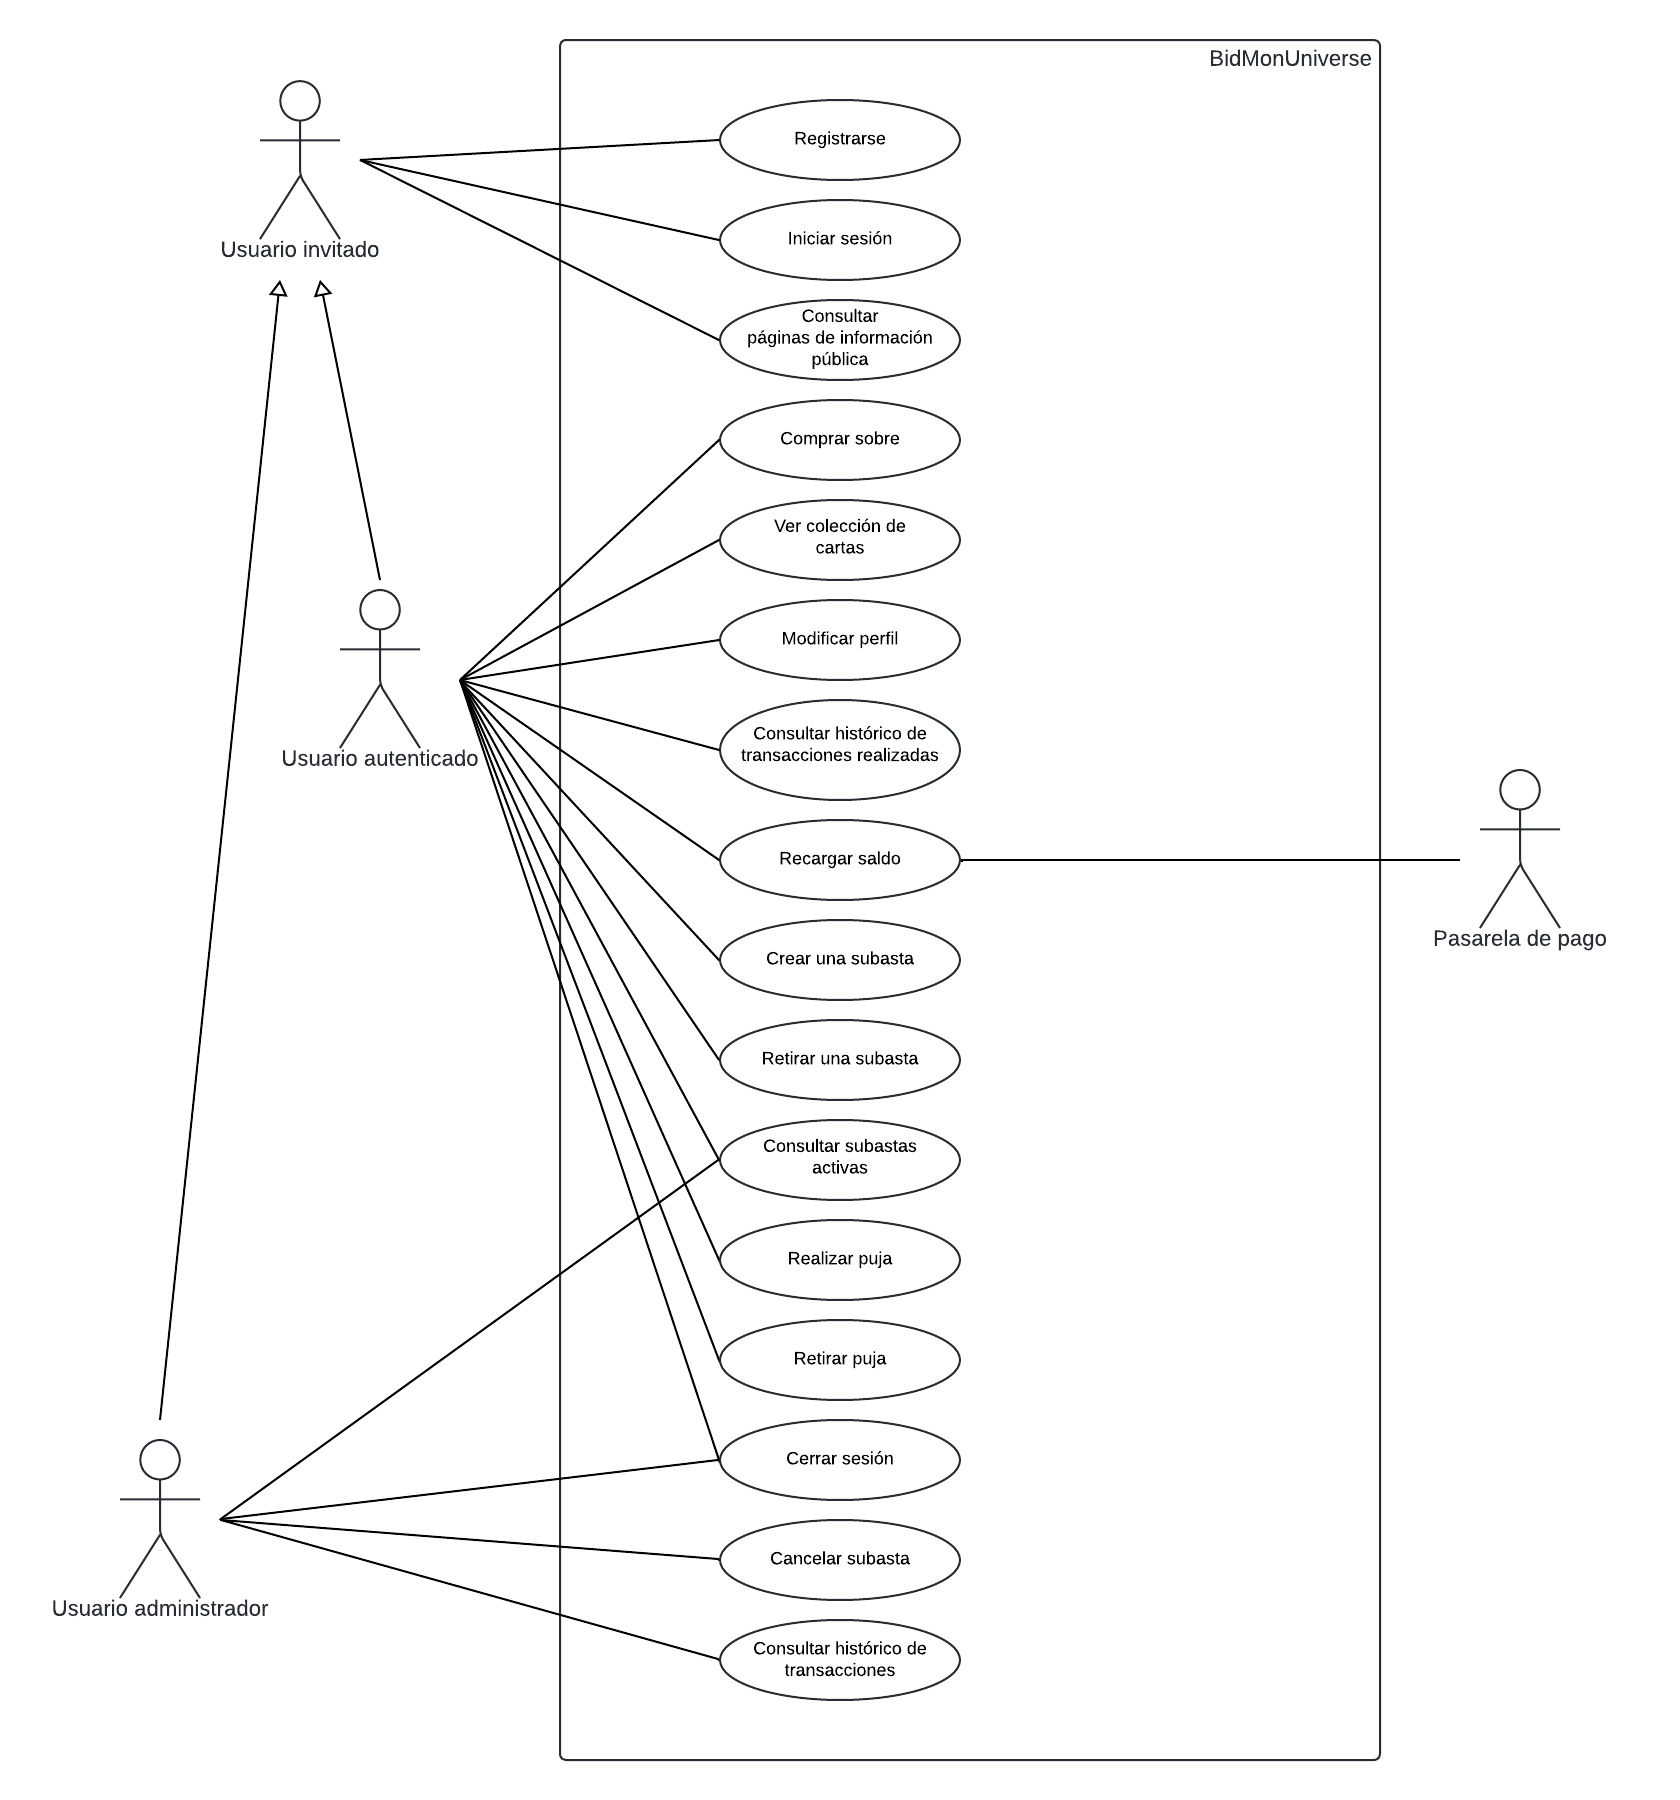
\includegraphics[width=1\textwidth]{figures/6-Analisis/6-Casos-uso/6_Diagrama-contexto.png}
    \caption{Diagrama de contexto del sistema}
    \label{fig:diagrama_contexto}
\end{figure}


\subsection{Casos de uso. Usuario invitado}

\begin{longtable}{
    >{\columncolor{lightgreen!20}}p{4cm}
    p{12cm}
    }
    \caption{Caso de uso. Registro} \label{table:cu_registro} \\
    \toprule
    \rowcolor{darkgreen!50}
    \textbf{Caso de uso} & \multicolumn{1}{>{\columncolor{darkgreen!50}\centering\arraybackslash}p{12cm}}{\textbf{REGISTRO}} \\
    \endfirsthead
    
    \multicolumn{2}{c}%
    {{ \tablename\ \thetable{} Caso de uso. Registro -- continuación de la página anterior}} \\
    \toprule
    \rowcolor{darkgreen!50}
    \textbf{Caso de uso} & \multicolumn{1}{>{\columncolor{darkgreen!50}\centering\arraybackslash}p{12cm}}{\textbf{REGISTRO}} \\
    \midrule
    \endhead
    
    \midrule
    \multicolumn{2}{r}{{Continúa en la siguiente página...}} \\ 
    \endfoot
    
    \bottomrule
    \endlastfoot
    
    \midrule
    Descripción & Un usuario invitado se puede registrar en el sistema para poder acceder a las funcionalidades del mismo. \\
    \midrule
    Actores principales & Usuario invitado \\
    \midrule
    Actores secundarios &  \\
    \midrule
    Precondiciones & El usuario no debe estar registrado en el sistema. \\
    \midrule
    Postcondiciones & \begin{itemize}[nosep,leftmargin=*]
      \item Se crea un nuevo registro en la base de datos con los datos del usuario.
      \item Se notifica al usuario que su registro ha sido exitoso.
      \item Se redirige al usuario a la página de inicio de sesión.
    \end{itemize} \\
    \midrule
    Disparadores & El usuario hace clic en el botón de registro. \\
    \midrule
    Escenario principal & \begin{enumerate}[nosep,leftmargin=*]
      \item El sistema muestra el formulario de registro.
      \item El usuario completa el formulario con sus datos personales.
      \item El usuario hace clic en el botón de registro.
      \item El sistema valida los datos del formulario.
      \item El sistema crea un nuevo registro en la base de datos con los datos del usuario.
      \item El sistema notifica al usuario que su registro ha sido exitoso.
      \item El sistema redirige al usuario a la página de inicio de sesión.
    \end{enumerate} \\
    \midrule
    Escenarios alternativos & 
    \begin{itemize}[nosep,leftmargin=*]
      \item Escenario alternativo 1. El usuario cancela el registro.
      \begin{enumerate}[nosep,leftmargin=*]
          \item El usuario hace clic en otro enlace.
          \item El sistema no crea el registro y redirige al usuario a la página correspondiente.
      \end{enumerate}
      \item Escenario alternativo 2. El usuario ya está registrado en el sistema.
      \begin{enumerate}[nosep,leftmargin=*]
          \item El sistema muestra un mensaje de error.
          \item El sistema no crea el registro y redirige al usuario de nuevo al formulario de registro.
      \end{enumerate}
      \item Escenario alternativo 3. El usuario no completa el formulario correctamente.
      \begin{enumerate}[nosep,leftmargin=*]
          \item El sistema muestra un mensaje de error con los campos que no se han completado correctamente.
          \item El sistema no crea el registro y redirige al usuario de nuevo al formulario de registro.
      \end{enumerate}
    \end{itemize} \\
    \midrule
    Situaciones de error & \begin{itemize}[nosep,leftmargin=*]
      \item Error 1. Error de conexión a la base de datos.
      \begin{enumerate}[nosep,leftmargin=*]
          \item El sistema muestra un mensaje de error.
          \item El sistema redirige al usuario de nuevo al formulario de registro.
      \end{enumerate}
    \end{itemize} \\
    \end{longtable}

\subsection{Casos de uso. Usuario autenticado}

\subsubsection{Caso de uso. Comprar sobre} \label{sec:cu_comprar-sobre}
\begin{longtable}{
    >{\columncolor{lightgreen!20}}p{4cm}
    p{12cm}
    }
    \caption{Caso de uso. Comprar sobre} \label{table:cu_comprar-sobre} \\
    \toprule
    \rowcolor{darkgreen!50}
    \textbf{Caso de uso} & \multicolumn{1}{>{\columncolor{darkgreen!50}\centering\arraybackslash}p{12cm}}{\textbf{COMPRAR SOBRE}} \\
    \endfirsthead
    
    \multicolumn{2}{c}%
    {{ \tablename\ \thetable{} Caso de uso. Comprar sobre -- continuación de la página anterior}} \\
    \toprule
    \rowcolor{darkgreen!50}
    \textbf{Caso de uso} & \multicolumn{1}{>{\columncolor{darkgreen!50}\centering\arraybackslash}p{12cm}}{\textbf{COMPRAR SOBRE}} \\
    \midrule
    \endhead
    
    \midrule
    \multicolumn{2}{r}{{Continúa en la siguiente página...}} \\ 
    \endfoot
    
    \bottomrule
    \endlastfoot
    
    \midrule
    Descripción & Un usuario autenticado puede comprar un sobre de cartas. \\
    \midrule
    Actores principales & Usuario autenticado \\
    \midrule
    Actores secundarios &  \\
    \midrule
    Precondiciones & \begin{itemize}[nosep,leftmargin=*]
        \item El usuario ha iniciado sesión en el sistema.
        \item El usuario dispone de saldo suficiente para comprar el sobre.
    \end{itemize} \\
    \midrule
    Postcondiciones & \begin{itemize}[nosep,leftmargin=*]
        \item Se descuenta el precio del sobre del saldo del usuario.
        \item Se añaden las cartas del sobre a la colección del usuario.
        \item Se decrementa en una unidad la cantidad de sobres disponibles en el inventario.
        \item Se registra la transacción en el historial de compras del usuario.
    \end{itemize} \\
    \midrule
    Disparadores & El usuario hace clic en el botón de comprar sobre. \\
    \midrule
    Escenario principal & \begin{enumerate}[nosep,leftmargin=*]
        \item El sistema muestra el inventario de sobres disponibles.
        \item El usuario selecciona el sobre que desea comprar.
        \item El usuario hace clic en el botón de comprar sobre.
        \item El sistema valida que el usuario dispone de saldo suficiente.
        \item El sistema descuenta el precio del sobre del saldo del usuario.
        \item El sistema genera las cartas del sobre.
        \item El sistema añade las cartas del sobre a la colección del usuario.
    \end{enumerate} \\
    \midrule
    Escenarios alternativos & 
    \begin{itemize}[nosep,leftmargin=*]
        \item \textbf{Escenario alternativo 1. El usuario intenta comprar un sobre sin saldo suficiente.}
        \begin{enumerate}[nosep,leftmargin=*]
            \item El usuario intenta comprar un sobre sin saldo suficiente.
            \item El sistema muestra un mensaje de error.
            \item El sistema le ofrece al usuario la posibilidad de recargar saldo.
        \end{enumerate}
    \end{itemize} \\
    \midrule
    Situaciones de error & 
    \begin{itemize}[nosep,leftmargin=*]
        \item \textbf{Error de conexión a la base de datos.}
        \begin{enumerate}[nosep,leftmargin=*]
            \item El sistema muestra un mensaje de error.
            \item El sistema no descuenta el precio del sobre del saldo del usuario.
            \item El sistema no añade las cartas del sobre a la colección del usuario.
            \item El sistema no decrementa en una unidad la cantidad de sobres disponibles en el inventario.
        \end{enumerate}
    \end{itemize} \\
\end{longtable}



\subsubsection{Caso de uso. Ver colección de cartas} \label{sec:cu_coleccion-cartas}
\begin{longtable}{
    >{\columncolor{lightgreen!20}}p{4cm}
    p{12cm}
    }
    \caption{Caso de uso. Ver colección de cartas} \label{table:cu_coleccion-cartas} \\
    \toprule
    \rowcolor{darkgreen!50}
    \textbf{Caso de uso} & \multicolumn{1}{>{\columncolor{darkgreen!50}\centering\arraybackslash}p{12cm}}{\textbf{VER COLECCIÓN DE CARTAS}} \\
    \endfirsthead
    
    \multicolumn{2}{c}%
    {{ \tablename\ \thetable{} Caso de uso. Ver colección de cartas -- continuación de la página anterior}} \\
    \toprule
    \rowcolor{darkgreen!50}
    \textbf{Caso de uso} & \multicolumn{1}{>{\columncolor{darkgreen!50}\centering\arraybackslash}p{12cm}}{\textbf{VER COLECCIÓN DE CARTAS}} \\
    \midrule
    \endhead
    
    \midrule
    \multicolumn{2}{r}{{Continúa en la siguiente página...}} \\ 
    \endfoot
    
    \bottomrule
    \endlastfoot
    
    \midrule
    Descripción & Un usuario autenticado puede ver la colección de cartas que posee. \\
    \midrule
    Actores principales & Usuario autenticado \\
    \midrule
    Actores secundarios &  \\
    \midrule
    Precondiciones & \begin{itemize}[nosep,leftmargin=*]
        \item El usuario debe haber iniciado sesión en el sistema.
    \end{itemize} \\
    \midrule
    Postcondiciones & \\
    \midrule
    Disparadores & El usuario accede a la sección de colección de cartas. \\
    \midrule
    Escenario principal & \begin{enumerate}[nosep,leftmargin=*]
        \item El sistema muestra la colección de cartas del usuario.
        \item El usuario puede seleccionar una carta para ver su información detallada.
    \end{enumerate} \\
    \midrule
    Escenarios alternativos & 
    \begin{itemize}[nosep,leftmargin=*]
        \item \textbf{Escenario alternativo 1. El usuario no tiene cartas en su colección.}
        \begin{enumerate}[nosep,leftmargin=*]
            \item Se mostrará un mensaje indicando que el usuario no tiene cartas en su colección.
            \item Se mostrará la opción de comprar un sobre de cartas o ir a la sección de subastas.
        \end{enumerate}
    \end{itemize} \\
    \midrule
    Situaciones de error & 
    \begin{itemize}[nosep,leftmargin=*]
        \item \textbf{Error de conexión a la base de datos.}
        \begin{enumerate}[nosep,leftmargin=*]
            \item El sistema mostrará un mensaje de error.
            \item El sistema le dará al usuario la opción de intentar cargar de nuevo la colección o volver a la página principal.
        \end{enumerate}
    \end{itemize} \\
\end{longtable}


\subsubsection{Caso de uso. Marcar carta como destacada} \label{sec:cu_carta-destacada}
\begin{longtable}{
    >{\columncolor{lightgreen!20}}p{4cm}
    p{12cm}
    }
    \caption{Caso de uso. Marcar carta como destacada} \label{table:cu_carta-destacada} \\
    \toprule
    \rowcolor{darkgreen!50}
    \textbf{Caso de uso} & \multicolumn{1}{>{\columncolor{darkgreen!50}\centering\arraybackslash}p{12cm}}{\textbf{MARCAR CARTA COMO DESTACADA}} \\
    \endfirsthead
    
    \multicolumn{2}{c}%
    {{ \tablename\ \thetable{} Caso de uso. Marcar carta como destacada -- continuación de la página anterior}} \\
    \toprule
    \rowcolor{darkgreen!50}
    \textbf{Caso de uso} & \multicolumn{1}{>{\columncolor{darkgreen!50}\centering\arraybackslash}p{12cm}}{\textbf{MARCAR CARTA COMO DESTACADA}} \\
    \midrule
    \endhead
    
    \midrule
    \multicolumn{2}{r}{{Continúa en la siguiente página...}} \\ 
    \endfoot
    
    \bottomrule
    \endlastfoot
    
    \midrule
    Descripción & Un usuario autenticado puede marcar una carta de su colección como destacada. \\
    \midrule
    Actores principales & Usuario autenticado \\
    \midrule
    Actores secundarios &  \\
    \midrule
    Precondiciones & \begin{itemize}[nosep,leftmargin=*]
        \item El usuario debe haber iniciado sesión en el sistema.
        \item El usuario debe tener al menos una carta en su colección.
    \end{itemize} \\
    \midrule
    Postcondiciones & \begin{itemize}[nosep,leftmargin=*]
        \item Se marca la carta como destacada en la base de datos.
    \end{itemize} \\
    \midrule
    Disparadores & El usuario accede a la sección de colección de cartas, selecciona una carta y la marca como destacada. \\
    \midrule
    Escenario principal & \begin{enumerate}[nosep,leftmargin=*]
        \item El sistema muestra la colección de cartas del usuario.
        \item El usuario puede seleccionar una carta para marcarla como destacada.
        \item El usuario hace clic en el botón de marcar como destacada.
        \item El sistema valida que el usuario no tenga ya una carta marcada como destacada.
        \item El sistema marca la carta como destacada en la base de datos.
        \item El sistema muestra un mensaje de éxito.
        \item El sistema redirige al usuario a la página que muestra su colección de cartas.
    \end{enumerate} \\
    \midrule
    Escenarios alternativos & 
    \begin{itemize}[nosep,leftmargin=*]
        \item \textbf{Escenario alternativo 1. El usuario ya tiene una carta marcada como destacada.}
        \begin{enumerate}[nosep,leftmargin=*]
            \item Se mostrará un mensaje indicando que el usuario ya tiene una carta marcada como destacada.
            \item Se mostrará la opción de desmarcar la carta actualmente destacada.
            \item Si el usuario confirma, se desmarcará la carta actualmente destacada y se marcará la nueva carta.
        \end{enumerate}
    \end{itemize} \\
    \midrule
    Situaciones de error & 
    \begin{itemize}[nosep,leftmargin=*]
        \item \textbf{Error de conexión a la base de datos.}
        \begin{enumerate}[nosep,leftmargin=*]
            \item El sistema mostrará un mensaje de error.
            \item El sistema no actualizará la carta como destacada en la base de datos.
            \item El sistema redirigirá al usuario a la página que muestra su colección de cartas.
        \end{enumerate}
    \end{itemize} \\
\end{longtable}




\subsubsection{Caso de uso. Modificar perfil} \label{sec:cu_modificar-perfil}
\begin{longtable}{
    >{\columncolor{lightgreen!20}}p{4cm}
    p{12cm}
    }
    \caption{Caso de uso. Modificar perfil} \label{table:cu_modificar-perfil} \\
    \toprule
    \rowcolor{darkgreen!50}
    \textbf{Caso de uso} & \multicolumn{1}{>{\columncolor{darkgreen!50}\centering\arraybackslash}p{12cm}}{\textbf{MODIFICAR PERFIL}} \\
    \endfirsthead
    
    \multicolumn{2}{c}%
    {{ \tablename\ \thetable{} Caso de uso. Modificar perfil -- continuación de la página anterior}} \\
    \toprule
    \rowcolor{darkgreen!50}
    \textbf{Caso de uso} & \multicolumn{1}{>{\columncolor{darkgreen!50}\centering\arraybackslash}p{12cm}}{\textbf{MODIFICAR PERFIL}} \\
    \midrule
    \endhead
    
    \midrule
    \multicolumn{2}{r}{{Continúa en la siguiente página...}} \\ 
    \endfoot
    
    \bottomrule
    \endlastfoot
    
    \midrule
    Descripción & Un usuario autenticado puede modificar su perfil de usuario. \\
    \midrule
    Actores principales & Usuario autenticado \\
    \midrule
    Actores secundarios &  \\
    \midrule
    Precondiciones & \begin{itemize}[nosep,leftmargin=*]
        \item El usuario debe haber iniciado sesión en el sistema.
    \end{itemize} \\
    \midrule
    Postcondiciones & \begin{itemize}[nosep,leftmargin=*]
        \item Se modifican los datos del perfil del usuario en la base de datos.
    \end{itemize} \\
    \midrule
    Disparadores & El usuario accede a la sección de modificar perfil. \\
    \midrule
    Escenario principal & \begin{enumerate}[nosep,leftmargin=*]
        \item El sistema muestra el formulario de modificación de perfil.
        \item El usuario modifica los campos que desee.
        \item El usuario hace clic en el botón de guardar cambios.
        \item El sistema valida los campos del formulario.
        \item El sistema actualiza los datos del perfil del usuario.
        \item El sistema muestra un mensaje de éxito.
        \item El sistema redirige al usuario a la página que muestra su perfil.
    \end{enumerate} \\
    \midrule
    Escenarios alternativos & 
    \begin{itemize}[nosep,leftmargin=*]
        \item \textbf{Escenario alternativo 1. El usuario cancela la modificación de perfil.}
        \begin{enumerate}[nosep,leftmargin=*]
            \item El usuario hace clic en el botón de cancelar.
            \item El sistema no modifica los datos del perfil del usuario.
            \item El sistema redirige al usuario a la página que muestra su perfil.
        \end{enumerate}
        \item \textbf{Escenario alternativo 2. El usuario introduce datos inválidos.}
        \begin{enumerate}[nosep,leftmargin=*]
            \item El sistema muestra un mensaje de error.
            \item El sistema no modifica los datos del perfil del usuario.
            \item El sistema muestra los campos con errores.
            \item El sistema permite al usuario corregir los errores.
        \end{enumerate}
    \end{itemize} \\
    \midrule
    Situaciones de error & 
    \begin{itemize}[nosep,leftmargin=*]
        \item \textbf{Error de conexión a la base de datos.}
        \begin{enumerate}[nosep,leftmargin=*]
            \item El sistema mostrará un mensaje de error.
            \item El sistema no modificará los datos del perfil del usuario.
            \item El sistema le dará al usuario la opción de intentar guardar de nuevo los cambios o volver a la página que muestra su perfil.
        \end{enumerate}
    \end{itemize} \\
\end{longtable}




\subsubsection{Caso de uso. Histórico de transacciones realizadas} \label{sec:cu_transacciones-realizadas}
\begin{longtable}{
    >{\columncolor{lightgreen!20}}p{4cm}
    >{\columncolor{white}}p{12cm} 
    }
    \caption{Caso de uso. Histórico de transacciones realizadas} \label{table:cu_transacciones-realizadas} \\
    \toprule
    \rowcolor{darkgreen!50}
    \textbf{Caso de uso} & \multicolumn{1}{>{\columncolor{darkgreen!50}\centering\arraybackslash}p{12cm}}{\textbf{HISTÓRICO DE TRANSACCIONES REALIZADAS}} \\
    \endfirsthead
    
    \multicolumn{2}{c}%
    {{ \tablename\ \thetable{} Caso de uso. Histórico de transacciones realizadas -- continuación de la página anterior}} \\
    \toprule
    \rowcolor{darkgreen!50}
    \textbf{Caso de uso} & \multicolumn{1}{>{\columncolor{darkgreen!50}\centering\arraybackslash}p{12cm}}{\textbf{HISTÓRICO DE TRANSACCIONES REALIZADAS}} \\
    \midrule
    \endhead
    
    \midrule
    \multicolumn{2}{r}{{Continúa en la siguiente página...}} \\ 
    \endfoot
    
    \bottomrule
    \endlastfoot
    
    \midrule
    Descripción & Un usuario autenticado puede consultar el histórico de transacciones realizadas en el sistema. \\
    \midrule
    Actores principales & Usuario autenticado \\
    \midrule
    Actores secundarios &  \\
    \midrule
    Precondiciones & \begin{itemize}[nosep,leftmargin=*]
        \item El usuario debe haber iniciado sesión en el sistema.
    \end{itemize} \\
    \midrule
    Postcondiciones & \\
    \midrule
    Disparadores & El usuario accede a la sección de historial de transacciones. \\
    \midrule
    Escenario principal & \begin{enumerate}[nosep,leftmargin=*]
        \item El sistema muestra el historial de transacciones del usuario.
    \end{enumerate} \\
    \midrule
    Escenarios alternativos & 
    \begin{itemize}[nosep,leftmargin=*]
        \item \textbf{Escenario alternativo 1. El usuario no tiene transacciones realizadas.}
        \begin{enumerate}[nosep,leftmargin=*]
            \item El sistema mostrará un mensaje indicando que el usuario no tiene transacciones realizadas.
        \end{enumerate}
    \end{itemize} \\
    \midrule
    Situaciones de error & 
    \begin{itemize}[nosep,leftmargin=*]
        \item \textbf{Error de conexión a la base de datos.}
        \begin{enumerate}[nosep,leftmargin=*]
            \item El sistema mostrará un mensaje de error.
            \item El sistema le dará al usuario la opción de intentar cargar de nuevo el historial de transacciones o volver a la página principal.
        \end{enumerate}
    \end{itemize} \\
\end{longtable}




\subsubsection{Caso de uso. Recargar saldo} \label{sec:cu_recarga-saldo}
\begin{longtable}{
    >{\columncolor{lightgreen!20}}p{4cm}
    p{12cm}
    }
    \caption{Caso de uso. Recargar saldo} \label{table:cu_recarga-saldo} \\
    \toprule
    \rowcolor{darkgreen!50}
    \textbf{Caso de uso} & \multicolumn{1}{>{\columncolor{darkgreen!50}\centering\arraybackslash}p{12cm}}{\textbf{RECRAGAR SALDO}} \\
    \endfirsthead
    
    \multicolumn{2}{c}%
    {{ \tablename\ \thetable{} Caso de uso. Recargar saldo -- continuación de la página anterior}} \\
    \toprule
    \rowcolor{darkgreen!50}
    \textbf{Caso de uso} & \multicolumn{1}{>{\columncolor{darkgreen!50}\centering\arraybackslash}p{12cm}}{\textbf{RECARGAR SALDO}} \\
    \midrule
    \endhead
    
    \midrule
    \multicolumn{2}{r}{{Continúa en la siguiente página...}} \\ 
    \endfoot
    
    \bottomrule
    \endlastfoot
    
    \midrule
    Descripción & Un usuario autenticado puede recargar saldo en su cuenta. \\
    \midrule
    Actores principales & Usuario autenticado \\
    \midrule
    Actores secundarios &  Pasarela de pago \\
    \midrule
    Precondiciones & \begin{itemize}[nosep,leftmargin=*]
        \item El usuario debe haber iniciado sesión en el sistema.
    \end{itemize} \\
    \midrule
    Postcondiciones & \begin{itemize}[nosep,leftmargin=*]
        \item Se incrementa el saldo del usuario en la base de datos.
    \end{itemize} \\
    \midrule
    Disparadores & El usuario accede a la sección de recarga de saldo. \\
    \midrule
    Escenario principal & \begin{enumerate}[nosep,leftmargin=*]
        \item El sistema muestra el formulario de recarga de saldo.
        \item El usuario introduce la cantidad de saldo que desea recargar.
        \item El usuario hace clic en el botón de recargar saldo.
        \item El sistema valida la cantidad de saldo introducida.
        \item El sistema redirige al usuario a la pasarela de pago.
        \item El usuario completa el pago.
        \item El sistema incrementa el saldo del usuario en la base de datos.
        \item El sistema muestra un mensaje de éxito.
    \end{enumerate} \\
    \midrule
    Escenarios alternativos & 
    \begin{itemize}[nosep,leftmargin=*]
        \item \textbf{Escenario alternativo 1. El usuario cancela la recarga de saldo en la pasarela de pago.}
        \begin{enumerate}[nosep,leftmargin=*]
            \item El usuario cancela el pago.
            \item El sistema no incrementa el saldo del usuario en la base de datos.
            \item El sistema redirige al usuario a la página que muestra su saldo actual.
            \item El sistema muestra un mensaje de cancelación.
        \end{enumerate}
        \item \textbf{Escenario alternativo 2. El usuario introduce una cantidad de saldo inválida.}
        \begin{enumerate}[nosep,leftmargin=*]
            \item El sistema muestra un mensaje de error.
            \item El sistema muestra los campos con errores.
            \item El sistema permite al usuario corregir los errores.
        \end{enumerate}
    \end{itemize} \\
    \midrule
    Situaciones de error & 
    \begin{itemize}[nosep,leftmargin=*]
        \item \textbf{Error de conexión a la base de datos.}
        \begin{enumerate}[nosep,leftmargin=*]
            \item El sistema mostrará un mensaje de error.
            \item El sistema no incrementará el saldo del usuario en la base de datos.
            \item El sistema le dará al usuario la opción de intentar recargar de nuevo el saldo o volver a la página de inicio.
        \end{enumerate}
        \item \textbf{Error en la pasarela de pago.}
        \begin{enumerate}[nosep,leftmargin=*]
            \item El sistema mostrará un mensaje de error.
            \item El sistema no incrementará el saldo del usuario en la base de datos.
            \item El sistema redirigirá al usuario a la página de recarga de saldo.
        \end{enumerate}
    \end{itemize} \\
\end{longtable}



\subsubsection{Caso de uso. Crear una subasta} \label{sec:cu_crear-subasta}
\begin{longtable}{
    >{\columncolor{lightgreen!20}}p{4cm}
    p{12cm}
    }
    \caption{Caso de uso. Crear una subasta} \label{table:cu_crear-subasta} \\
    \toprule
    \rowcolor{darkgreen!50}
    \textbf{Caso de uso} & \multicolumn{1}{>{\columncolor{darkgreen!50}\centering\arraybackslash}p{12cm}}{\textbf{CREAR UNA SUBASTA}} \\
    \endfirsthead
    
    \multicolumn{2}{c}%
    {{ \tablename\ \thetable{} Caso de uso. Crear una subasta -- continuación de la página anterior}} \\
    \toprule
    \rowcolor{darkgreen!50}
    \textbf{Caso de uso} & \multicolumn{1}{>{\columncolor{darkgreen!50}\centering\arraybackslash}p{12cm}}{\textbf{CREAR UNA SUBASTA}} \\
    \midrule
    \endhead
    
    \midrule
    \multicolumn{2}{r}{{Continúa en la siguiente página...}} \\ 
    \endfoot
    
    \bottomrule
    \endlastfoot
    
    \midrule
    Descripción & Un usuario autenticado puede crear una subasta de una carta de su colección. \\
    \midrule
    Actores principales & Usuario autenticado \\
    \midrule
    Actores secundarios &  \\
    \midrule
    Precondiciones & \begin{itemize}[nosep,leftmargin=*]
        \item El usuario debe haber iniciado sesión en el sistema.
        \item El usuario debe tener al menos una carta en su colección.
        \item El usuario no debe tener ya una subasta activa para la carta que desea subastar.
    \end{itemize} \\
    \midrule
    Postcondiciones & \begin{itemize}[nosep,leftmargin=*]
        \item Se crea una nueva subasta en la base de datos.
        \item Se marca la carta como 'en subasta' en la base de datos.
    \end{itemize} \\
    \midrule
    Disparadores & El usuario accede a la sección de subastas y hace clic en el botón de crear subasta. \\
    \midrule
    Escenario principal & \begin{enumerate}[nosep,leftmargin=*]
        \item El sistema muestra el formulario de creación de subasta.
        \item El usuario selecciona la carta que desea subastar.
        \item El usuario introduce el precio de salida y la duración de la subasta.
        \item El usuario hace clic en el botón de crear subasta.
        \item El sistema valida los campos del formulario.
        \item El sistema crea una nueva subasta en la base de datos.
        \item El sistema marca la carta como 'en subasta' en la base de datos.
        \item El sistema muestra un mensaje de éxito.
        \item El sistema redirige al usuario a la página de subastas.
        \item El sistema muestra la subasta creada en la lista de subastas.
    \end{enumerate} \\
    \midrule
    Escenarios alternativos & 
    \begin{itemize}[nosep,leftmargin=*]
        \item \textbf{Escenario alternativo 1. El usuario ya tiene una subasta activa para la carta que desea subastar.}
        \begin{enumerate}[nosep,leftmargin=*]
            \item El usuario intenta crear una subasta para una carta que ya está en subasta.
            \item El sistema muestra un mensaje de error.
            \item El sistema redirige al usuario a la página de subastas.
        \end{enumerate}
        \item \textbf{Escenario alternativo 2. El usuario introduce datos inválidos.}
        \begin{enumerate}[nosep,leftmargin=*]
            \item El sistema muestra un mensaje de error.
            \item El sistema no crea la subasta en la base de datos.
            \item El sistema no marcará la carta como 'en subasta' en la base de datos.
            \item El sistema le mostrará al usuario los campos con errores.
            \item El sistema permitirá al usuario corregir los errores.
        \end{enumerate}
    \end{itemize} \\
    \midrule
    Situaciones de error & 
    \begin{itemize}[nosep,leftmargin=*]
        \item \textbf{Error de conexión a la base de datos.}
        \begin{enumerate}[nosep,leftmargin=*]
            \item El sistema mostrará un mensaje de error.
            \item El sistema no creará la subasta en la base de datos.
            \item El sistema no marcará la carta como 'en subasta' en la base de datos.
            \item El sistema redirigirá al usuario a la página de subastas.
        \end{enumerate}
    \end{itemize} \\
\end{longtable}




\subsubsection{Caso de uso. Retirar una subasta} \label{sec:cu_retirar-subasta}
\begin{longtable}{
    >{\columncolor{lightgreen!20}}p{4cm}
    p{12cm}
    }
    \caption{Caso de uso. Retirar una subasta} \label{table:cu_retirar-subasta} \\
    \toprule
    \rowcolor{darkgreen!50}
    \textbf{Caso de uso} & \multicolumn{1}{>{\columncolor{darkgreen!50}\centering\arraybackslash}p{12cm}}{\textbf{RETIRAR UNA SUBASTA}} \\
    \endfirsthead
    
    \multicolumn{2}{c}%
    {{ \tablename\ \thetable{} Caso de uso. Retirar una subasta -- continuación de la página anterior}} \\
    \toprule
    \rowcolor{darkgreen!50}
    \textbf{Caso de uso} & \multicolumn{1}{>{\columncolor{darkgreen!50}\centering\arraybackslash}p{12cm}}{\textbf{RETIRAR UNA SUBASTA}} \\
    \midrule
    \endhead
    
    \midrule
    \multicolumn{2}{r}{{Continúa en la siguiente página...}} \\ 
    \endfoot
    
    \bottomrule
    \endlastfoot
    
    \midrule
    Descripción & Un usuario  \\
    \midrule
    Actores principales & Usuario autenticado \\
    \midrule
    Actores secundarios &  \\
    \midrule
    Precondiciones & \begin{itemize}[nosep,leftmargin=*]
        \item El usuario debe haber iniciado sesión en el sistema.
        \item El usuario debe tener al menos una subasta activa.
    \end{itemize} \\
    \midrule
    Postcondiciones & \begin{itemize}[nosep,leftmargin=*]
        \item Se marca la subasta como 'cancelada' en la base de datos.
        \item La carta subastada vuelve a estar disponible en la colección del usuario.
        \item Se actualizan las pujas de la subasta en la base de datos, marcando las pujas como 'canceladas'.
        \item Se informa a los usuarios que hayan pujado en la subasta de que ha sido cancelada.
    \end{itemize} \\
    \midrule
    Disparadores & El usuario accede a la sección de subastas y hace clic en el botón de retirar subasta. \\
    \midrule
    Escenario principal & \begin{enumerate}[nosep,leftmargin=*]
        \item El sistema muestra la lista de subastas activas del usuario.
        \item El usuario selecciona la subasta que desea retirar.
        \item El usuario hace clic en el botón de retirar subasta.
        \item El sistema muestra un mensaje de confirmación.
        \item El usuario confirma la retirada de la subasta.
        \item El sistema marca la subasta como 'cancelada' en la base de datos.
        \item La carta subastada vuelve a estar disponible en la colección del usuario.
        \item El sistema muestra un mensaje de éxito.
        \item El sistema redirige al usuario a la página de subastas.
    \end{enumerate} \\
    \midrule
    Escenarios alternativos & 
    \begin{itemize}[nosep,leftmargin=*]
        \item \textbf{Escenario alternativo 1. El usuario cancela la retirada de la subasta.}
        \begin{enumerate}[nosep,leftmargin=*]
            \item El usuario hace clic en el botón de cancelar en el mensaje de confirmación.
            \item El sistema no marcará la subasta como 'cancelada' en la base de datos.
            \item El sistema redirigirá al usuario a la página de subastas.
        \end{enumerate}
    \end{itemize} \\
    \midrule
    Situaciones de error & 
    \begin{itemize}[nosep,leftmargin=*]
        \item \textbf{Error de conexión a la base de datos.}
        \begin{enumerate}[nosep,leftmargin=*]
            \item El sistema mostrará un mensaje de error.
            \item El sistema no marcará la subasta como 'cancelada' en la base de datos.
            \item El sistema no devolverá la carta subastada a la colección del usuario.
            \item El sistema redirigirá al usuario a la página de subastas.
        \end{enumerate}
    \end{itemize} \\
\end{longtable}




\subsubsection{Caso de uso. Consultar subastas activas} \label{sec:cu_consultar-subastas}
\begin{longtable}{
    >{\columncolor{lightgreen!20}}p{4cm}
    p{12cm}
    }
    \caption{Caso de uso. Consultar subastas activas} \label{table:cu_consultar-subastas} \\
    \toprule
    \rowcolor{darkgreen!50}
    \textbf{Caso de uso} & \multicolumn{1}{>{\columncolor{darkgreen!50}\centering\arraybackslash}p{12cm}}{\textbf{CONSULTAR SUBASTAS ACTIVAS}} \\
    \endfirsthead
    
    \multicolumn{2}{c}%
    {{ \tablename\ \thetable{} Caso de uso. Consultar subastas activas -- continuación de la página anterior}} \\
    \toprule
    \rowcolor{darkgreen!50}
    \textbf{Caso de uso} & \multicolumn{1}{>{\columncolor{darkgreen!50}\centering\arraybackslash}p{12cm}}{\textbf{CONSULTAR SUBASTAS ACTIVAS}} \\
    \midrule
    \endhead
    
    \midrule
    \multicolumn{2}{r}{{Continúa en la siguiente página...}} \\ 
    \endfoot
    
    \bottomrule
    \endlastfoot
    
    \midrule
    Descripción & Un usuario  \\
    \midrule
    Actores principales & Usuario autenticado o usuario administrador \\
    \midrule
    Actores secundarios &  \\
    \midrule
    Precondiciones & \begin{itemize}[nosep,leftmargin=*]
        \item El usuario debe haber iniciado sesión en el sistema.
    \end{itemize} \\
    \midrule
    Postcondiciones &  \\
    \midrule
    Disparadores & El usuario accede a la sección de subastas. \\
    \midrule
    Escenario principal & \begin{enumerate}[nosep,leftmargin=*]
        \item El sistema muestra la lista de subastas activas.
        \item El usuario puede seleccionar una subasta para ver su información detallada.
    \end{enumerate} \\
    \midrule
    Escenarios alternativos & 
    \begin{itemize}[nosep,leftmargin=*]
        \item \textbf{Escenario alternativo 1. No hay subastas activas.}
        \begin{enumerate}[nosep,leftmargin=*]
            \item El sistema mostrará un mensaje indicando que no hay subastas activas.
        \end{enumerate}
        \item \textbf{Escenario alternativo 2. El usuario consulta sus propias subastas.} 
        \begin{enumerate}[nosep,leftmargin=*]
            \item El usuario accede a la sección de subastas.
            \item El sistema muestra la opción de ver las subastas activas del usuario.
            \item El usuario selecciona la opción de ver sus propias subastas.
            \item El sistema muestra la lista de subastas activas del usuario.
        \end{enumerate}
        \item \textbf{Escenario alternativo 3. Un usuario administrador consulta las subastas activas.}
        \begin{enumerate}[nosep,leftmargin=*]
            \item El usuario administrador accede a la sección de subastas.
            \item El sistema muestra la lista de subastas activas de todos los usuarios.
            \item El usuario administrador puede seleccionar una subasta para ver su información detallada.
            \item El usuario administrador puede seleccionar una subasta para cancelarla.
        \end{enumerate}
    \end{itemize} \\
    \midrule
    Situaciones de error & 
    \begin{itemize}[nosep,leftmargin=*]
        \item \textbf{Error de conexión a la base de datos.}
        \begin{enumerate}[nosep,leftmargin=*]
            \item El sistema mostrará un mensaje de error.
        \end{enumerate}
    \end{itemize} \\
\end{longtable}



\subsubsection{Caso de uso. Realizar puja} \label{sec:cu_realizar-puja}
\begin{longtable}{
    >{\columncolor{lightgreen!20}}p{4cm}
    p{12cm}
    }
    \caption{Caso de uso. Realizar puja} \label{table:cu_realizar-puja} \\
    \toprule
    \rowcolor{darkgreen!50}
    \textbf{Caso de uso} & \multicolumn{1}{>{\columncolor{darkgreen!50}\centering\arraybackslash}p{12cm}}{\textbf{REALIZAR PUJA}} \\
    \endfirsthead
    
    \multicolumn{2}{c}%
    {{ \tablename\ \thetable{} Caso de uso. Realizar puja -- continuación de la página anterior}} \\
    \toprule
    \rowcolor{darkgreen!50}
    \textbf{Caso de uso} & \multicolumn{1}{>{\columncolor{darkgreen!50}\centering\arraybackslash}p{12cm}}{\textbf{REALIZAR PUJA}} \\
    \midrule
    \endhead
    
    \midrule
    \multicolumn{2}{r}{{Continúa en la siguiente página...}} \\ 
    \endfoot
    
    \bottomrule
    \endlastfoot
    
    \midrule
    Descripción & Un usuario autenticado puede realizar una puja en una subasta activa. \\
    \midrule
    Actores principales & Usuario autenticado \\
    \midrule
    Actores secundarios &  \\
    \midrule
    Precondiciones & \begin{itemize}[nosep,leftmargin=*]
        \item El usuario debe haber iniciado sesión en el sistema.
        \item El usuario debe tener saldo suficiente para realizar la puja.
    \end{itemize} \\
    \midrule
    Postcondiciones & \begin{itemize}[nosep,leftmargin=*]
        \item Se registra la puja en la base de datos.
    \end{itemize} \\
    \midrule
    Disparadores & El usuario selecciona una subasta activa y hace clic en el botón de realizar puja. \\
    \midrule
    Escenario principal & \begin{enumerate}[nosep,leftmargin=*]
        \item El sistema muestra la información detallada de la subasta.
        \item El usuario introduce la cantidad de la puja.
        \item El usuario hace clic en el botón de realizar puja.
        \item El sistema valida la cantidad de la puja.
        \item El sistema registra la puja en la base de datos.
        \item El sistema muestra un mensaje de éxito.
        \item El sistema muestra un mensaje informativo, indicando que si en el momento de finalización del tiempo de la subasta no cuenta con el saldo suficiente, la puja no será válida.
        \item El sistema redirige al usuario a la página de subastas.
    \end{enumerate} \\
    \midrule
    Escenarios alternativos & 
    \begin{itemize}[nosep,leftmargin=*]
        \item \textbf{Escenario alternativo 1. El usuario no tiene saldo suficiente para realizar la puja.}
        \begin{enumerate}[nosep,leftmargin=*]
            \item El usuario intenta realizar una puja sin tener saldo suficiente.
            \item El sistema mostrará un mensaje de error.
            \item El sistema no registrará la puja en la base de datos.
            \item El sistema redirigirá al usuario a la página de subastas.
        \end{enumerate}
        \item \textbf{Escenario alternativo 2. El usuario introduce una cantidad de puja inválida.}
        \begin{enumerate}[nosep,leftmargin=*]
            \item El sistema mostrará un mensaje de error.
            \item El sistema no registrará la puja en la base de datos.
            \item El sistema le mostrará al usuario los campos con errores.
            \item El sistema permitirá al usuario corregir los errores.
        \end{enumerate}
    \end{itemize} \\
    \midrule
    Situaciones de error & 
    \begin{itemize}[nosep,leftmargin=*]
        \item \textbf{Error de conexión a la base de datos.}
        \begin{enumerate}[nosep,leftmargin=*]
            \item El sistema mostrará un mensaje de error.
            \item El sistema no registrará la puja en la base de datos.
            \item El sistema redirigirá al usuario a la página de subastas.
        \end{enumerate}
    \end{itemize} \\
\end{longtable}



\subsubsection{Caso de uso. Retirar puja} \label{sec:cu_retirar-puja}
\begin{longtable}{
    >{\columncolor{lightgreen!20}}p{4cm}
    p{12cm}
    }
    \caption{Caso de uso. Retirar puja} \label{table:cu_retirar-puja} \\
    \toprule
    \rowcolor{darkgreen!50}
    \textbf{Caso de uso} & \multicolumn{1}{>{\columncolor{darkgreen!50}\centering\arraybackslash}p{12cm}}{\textbf{RETIRAR PUJA}} \\
    \endfirsthead
    
    \multicolumn{2}{c}%
    {{ \tablename\ \thetable{} Caso de uso. Retirar puja -- continuación de la página anterior}} \\
    \toprule
    \rowcolor{darkgreen!50}
    \textbf{Caso de uso} & \multicolumn{1}{>{\columncolor{darkgreen!50}\centering\arraybackslash}p{12cm}}{\textbf{RETIRAR PUJA}} \\
    \midrule
    \endhead
    
    \midrule
    \multicolumn{2}{r}{{Continúa en la siguiente página...}} \\ 
    \endfoot
    
    \bottomrule
    \endlastfoot
    
    \midrule
    Descripción & Un usuario podrá retirar una puja realizada en una subasta activa. \\
    \midrule
    Actores principales & Usuario autenticado \\
    \midrule
    Actores secundarios &  \\
    \midrule
    Precondiciones & \begin{itemize}[nosep,leftmargin=*]
        \item El usuario debe haber iniciado sesión en el sistema.
        \item El usuario debe haber realizado una puja en una subasta activa.
        \item La subasta no debe haber finalizado.
    \end{itemize} \\
    \midrule
    Postcondiciones & \begin{itemize}[nosep,leftmargin=*]
        \item Se actualiza la puja en la base de datos, marcándola como 'retirada'.
        \item La puja no se muestra en la lista de pujas activas del usuario.
        \item La puja no se tendr´a en cuenta en el cálculo de la puja más alta.
    \end{itemize} \\
    \midrule
    Disparadores & El usuario accede a la sección de pujas activas, selecciona una puja y hace clic en el botón de retirar puja. \\
    \midrule
    Escenario principal & \begin{enumerate}[nosep,leftmargin=*]
        \item El sistema muestra la lista de pujas activas del usuario.
        \item El usuario selecciona la puja que desea retirar.
        \item El usuario hace clic en el botón de retirar puja.
        \item El sistema muestra un mensaje de confirmación.
        \item El usuario confirma la retirada de la puja.
        \item El sistema actualiza la puja en la base de datos, marcándola como 'retirada'.
        \item El sistema muestra un mensaje de éxito.
        \item El sistema redirige al usuario a la página de subastas.
    \end{enumerate} \\
    \midrule
    Escenarios alternativos & 
    \begin{itemize}[nosep,leftmargin=*]
        \item \textbf{Escenario alternativo 1. El usuario cancela la retirada de la puja.}
        \begin{enumerate}[nosep,leftmargin=*]
            \item El usuario hace clic en el botón de cancelar en el mensaje de confirmación.
            \item El sistema no marcará la puja como 'retirada' en la base de datos.
            \item El sistema redirigirá al usuario a la página de subastas.
        \end{enumerate}
    \end{itemize} \\
    \midrule
    Situaciones de error & 
    \begin{itemize}[nosep,leftmargin=*]
        \item \textbf{Error de conexión a la base de datos.}
        \begin{enumerate}[nosep,leftmargin=*]
            \item El sistema mostrará un mensaje de error.
            \item El sistema redirigirá al usuario a la página de subastas.
        \end{enumerate}
    \end{itemize} \\
\end{longtable}



\subsubsection{Caso de uso. Consultar pujas activas} \label{sec:cu_consultar-pujas}
\begin{longtable}{
    >{\columncolor{lightgreen!20}}p{4cm}
    p{12cm}
    }
    \caption{Caso de uso. Consultar pujas activas} \label{table:cu_consultar-puja} \\
    \toprule
    \rowcolor{darkgreen!50}
    \textbf{Caso de uso} & \multicolumn{1}{>{\columncolor{darkgreen!50}\centering\arraybackslash}p{12cm}}{\textbf{CONSULTAR PUJAS ACTIVAS}} \\
    \endfirsthead
    
    \multicolumn{2}{c}%
    {{ \tablename\ \thetable{} Caso de uso. Consultar pujas activas -- continuación de la página anterior}} \\
    \toprule
    \rowcolor{darkgreen!50}
    \textbf{Caso de uso} & \multicolumn{1}{>{\columncolor{darkgreen!50}\centering\arraybackslash}p{12cm}}{\textbf{CONSULTAR PUJAS ACTIVAS}} \\
    \midrule
    \endhead
    
    \midrule
    \multicolumn{2}{r}{{Continúa en la siguiente página...}} \\ 
    \endfoot
    
    \bottomrule
    \endlastfoot
    
    \midrule
    Descripción & Un usuario  \\
    \midrule
    Actores principales & Usuario autenticado \\
    \midrule
    Actores secundarios &  \\
    \midrule
    Precondiciones & \begin{itemize}[nosep,leftmargin=*]
        \item El usuario debe haber iniciado sesión en el sistema.
    \end{itemize} \\
    \midrule
    Postcondiciones & \\
    \midrule
    Disparadores & El usuario accede a la sección de subastas y hace clic en el botón de ver pujas activas. \\
    \midrule
    Escenario principal & \begin{enumerate}[nosep,leftmargin=*]
        \item El sistema muestra la lista de pujas activas del usuario.
    \end{enumerate} \\
    \midrule
    Escenarios alternativos & 
    \begin{itemize}[nosep,leftmargin=*]
        \item \textbf{Escenario alternativo 1. No hay pujas activas.}
        \begin{enumerate}[nosep,leftmargin=*]
            \item El sistema mostrará un mensaje indicando que no hay pujas activas.
        \end{enumerate}
    \end{itemize} \\
    \midrule
    Situaciones de error & 
    \begin{itemize}[nosep,leftmargin=*]
        \item \textbf{Error de conexión a la base de datos.}
        \begin{enumerate}[nosep,leftmargin=*]
            \item El sistema mostrará un mensaje de error.
        \end{enumerate}
    \end{itemize} \\
\end{longtable}



\subsubsection{Caso de uso. Cerrar sesión} \label{sec:cu_cerrar-sesion}
\begin{longtable}{
    >{\columncolor{lightgreen!20}}p{4cm}
    p{12cm}
    }
    \caption{Caso de uso. Cerrar sesión} \label{table:cu_cerrar-sesion} \\
    \toprule
    \rowcolor{darkgreen!50}
    \textbf{Caso de uso} & \multicolumn{1}{>{\columncolor{darkgreen!50}\centering\arraybackslash}p{12cm}}{\textbf{CERRAR SESIÓN}} \\
    \endfirsthead
    
    \multicolumn{2}{c}%
    {{ \tablename\ \thetable{} Caso de uso. Cerrar sesión -- continuación de la página anterior}} \\
    \toprule
    \rowcolor{darkgreen!50}
    \textbf{Caso de uso} & \multicolumn{1}{>{\columncolor{darkgreen!50}\centering\arraybackslash}p{12cm}}{\textbf{CERRAR SESIÓN}} \\
    \midrule
    \endhead
    
    \midrule
    \multicolumn{2}{r}{{Continúa en la siguiente página...}} \\ 
    \endfoot
    
    \bottomrule
    \endlastfoot
    
    \midrule
    Descripción & Un usuario puede cerrar sesión en el sistema si previamente ha iniciado sesión. \\
    \midrule
    Actores principales & Usuario autenticado o usuario administrador \\
    \midrule
    Actores secundarios &  \\
    \midrule
    Precondiciones & \begin{itemize}[nosep,leftmargin=*]
        \item El usuario debe haber iniciado sesión en el sistema.
    \end{itemize} \\
    \midrule
    Postcondiciones & \begin{itemize}[nosep,leftmargin=*]
        \item Se elimina la sesión del usuario.
    \end{itemize} \\
    \midrule
    Disparadores & El usuario hace clic en el botón de cerrar sesión. \\
    \midrule
    Escenario principal & \begin{enumerate}[nosep,leftmargin=*]
        \item El usuario hace clic en el botón de cerrar sesión.
        \item El sistema elimina la sesión del usuario.
        \item El sistema redirige al usuario a la página de inicio.
    \end{enumerate} \\
    \midrule
    Escenarios alternativos &  \\
    \midrule
    Situaciones de error &  \\
\end{longtable}

\subsection{Casos de uso. Usuario administrador}

\subsubsection{Caso de uso. Histórico de transacciones del sistema} \label{sec:cu_transacciones-sistema}
\begin{longtable}{
    >{\columncolor{lightgreen!20}}p{4cm}
    p{12cm}
    }
    \caption{Caso de uso. Histórico de transacciones del sistema} \label{table:cu_transacciones-sistema} \\
    \toprule
    \rowcolor{darkgreen!50}
    \textbf{Caso de uso} & \multicolumn{1}{>{\columncolor{darkgreen!50}\centering\arraybackslash}p{12cm}}{\textbf{HISTÓRICO DE TRANSACCIONES DEL SISTEMA}} \\
    \endfirsthead
    
    \multicolumn{2}{c}%
    {{ \tablename\ \thetable{} Caso de uso. Histórico de transacciones del sistema -- continuación de la página anterior}} \\
    \toprule
    \rowcolor{darkgreen!50}
    \textbf{Caso de uso} & \multicolumn{1}{>{\columncolor{darkgreen!50}\centering\arraybackslash}p{12cm}}{\textbf{HISTÓRICO DE TRANSACCIONES DEL SISTEMA}} \\
    \midrule
    \endhead
    
    \midrule
    \multicolumn{2}{r}{{Continúa en la siguiente página...}} \\ 
    \endfoot
    
    \bottomrule
    \endlastfoot
    
    \midrule
    Descripción & Un usuario administrador puede consultar el histórico de transacciones del sistema. \\
    \midrule
    Actores principales & Usuario administrador \\
    \midrule
    Actores secundarios &  \\
    \midrule
    Precondiciones & \begin{itemize}[nosep,leftmargin=*]
        \item El usuario ha iniciado sesión en el sistema.
    \end{itemize} \\
    \midrule
    Postcondiciones &  \\
    \midrule
    Disparadores & El usuario selecciona la opción de consultar el histórico de transacciones. \\
    \midrule
    Escenario principal & \begin{enumerate}[nosep,leftmargin=*]
        \item El sistema muestra el listado de transacciones realizadas en el sistema por los diferentes usuarios.
    \end{enumerate} \\
    \midrule
    Escenarios alternativos & 
    \begin{itemize}[nosep,leftmargin=*]
        \item \textbf{Escenario alternativo 1. No hay transacciones registradas.}
        \begin{enumerate}[nosep,leftmargin=*]
            \item El sistema muestra un mensaje indicando que no hay transacciones registradas.
        \end{enumerate}
    \end{itemize} \\
    \midrule
    Situaciones de error & 
    \begin{itemize}[nosep,leftmargin=*]
        \item \textbf{Error de conexión a la base de datos.}
        \begin{enumerate}[nosep,leftmargin=*]
            \item El sistema muestra un mensaje de error.
        \end{enumerate}
    \end{itemize} \\
\end{longtable}



\subsubsection{Caso de uso. Cancelar subasta activa} \label{sec:cu_cancelar-subasta}
\begin{longtable}{
    >{\columncolor{lightgreen!20}}p{4cm}
    p{12cm}
    }
    \caption{Caso de uso. Cancelar subasta activa} \label{table:cu_cancelar-subasta} \\
    \toprule
    \rowcolor{darkgreen!50}
    \textbf{Caso de uso} & \multicolumn{1}{>{\columncolor{darkgreen!50}\centering\arraybackslash}p{12cm}}{\textbf{CANCELAR SUBASTA ACTIVA}} \\
    \endfirsthead
    
    \multicolumn{2}{c}%
    {{ \tablename\ \thetable{} Caso de uso. Cancelar subasta activa -- continuación de la página anterior}} \\
    \toprule
    \rowcolor{darkgreen!50}
    \textbf{Caso de uso} & \multicolumn{1}{>{\columncolor{darkgreen!50}\centering\arraybackslash}p{12cm}}{\textbf{CANCELAR SUBASTA ACTIVA}} \\
    \midrule
    \endhead
    
    \midrule
    \multicolumn{2}{r}{{Continúa en la siguiente página...}} \\ 
    \endfoot
    
    \bottomrule
    \endlastfoot
    
    \midrule
    Descripción & Un usuario administrador puede cancelar una subasta activa en el sistema. \\
    \midrule
    Actores principales & Usuario administrador \\
    \midrule
    Actores secundarios &  \\
    \midrule
    Precondiciones & \begin{itemize}[nosep,leftmargin=*]
        \item El usuario ha iniciado sesión en el sistema.
        \item Existe una subasta activa en el sistema.
    \end{itemize} \\
    \midrule
    Postcondiciones & \begin{itemize}[nosep,leftmargin=*]
        \item Se actualiza el estado de la subasta a cancelada en la base de datos.
        \item Se actualizan las pujas realizadas en la subasta cancelada en la base de datos, marcándolas como 'canceladas'.
        \item Se notifica a los usuarios participantes en la subasta de la cancelación.
    \end{itemize} \\
    \midrule
    Disparadores & El usuario selecciona la opción de cancelar una subasta activa. \\
    \midrule
    Escenario principal & \begin{enumerate}[nosep,leftmargin=*]
        \item El sistema muestra el listado de subastas activas en el sistema.
        \item El usuario selecciona la subasta que desea cancelar.
        \item El sistema muestra un mensaje de confirmación de la cancelación.
        \item El usuario confirma la cancelación de la subasta.
        \item El sistema actualiza el estado de la subasta a cancelada en la base de datos.
        \item El sistema actualiza las pujas realizadas en la subasta cancelada en la base de datos, marcándolas como 'canceladas'.
        \item El sistema notifica a los usuarios participantes en la subasta de la cancelación.
        \item El sistema redirige al usuario al listado de subastas activas.
    \end{enumerate} \\
    \midrule
    Escenarios alternativos & \\
    \midrule
    Situaciones de error & 
    \begin{itemize}[nosep,leftmargin=*]
        \item \textbf{Error de conexión a la base de datos.}
        \begin{enumerate}[nosep,leftmargin=*]
            \item El sistema muestra un mensaje de error.
        \end{enumerate}
    \end{itemize} \\
\end{longtable}

\newpage
\section{IDENTIFICACIÓN DE SUBSISTEMAS DE ANÁLISIS} \label{sec:identificacion-subsistemas-analisis} \hypertarget{sec:identificacion-subsistemas-analisis}
% 6.3. Identificación de subsistemas de análisis + 7.3. Diseño de la Arquitectura de Módulos del Sistema

\subsection{Descripción de los Subsistemas} 

\subsection{Descripción de los Interfaces entre Subsistemas}



\newpage
\section{ARQUITECTURA DE LOS SUBSISTEMAS DE ANÁLISIS}
% 6.5. Análisis de clases + 7.2 Diseño de Clases

En este apartado se detalla la arquitectura de los subsistemas de análisis. Como se ha visto en el apartado anterior, el sistema se divide en dos subsistemas principales: 
\textbf{restapi} y \textbf{frontend}. El subsistema restapi contiene las clases que implementan la API REST y la lógica de negocio, mientras que el subsistema frontend abarca la interfaz de usuario.

Primero, se presentará el diagrama de paquetes para ofrecer una visión general de la estructura del sistema. Este diagrama ilustrará la organización y 
agrupación de los distintos elementos del sistema en paquetes, permitiendo una comprensión clara de su disposición y jerarquía.

A continuación, se analizará cada subsistema en detalle mediante un diagrama de componentes por cada subsistema. Se ha optado por un diagrama de componentes debido a que el sistema sigue una arquitectura MERN 
(MongoDB, Express, React, Node.js) y este tipo de diagrama aporta más valor que un diagrama de clases al reflejar más fielmente la estructura y relaciones entre los distintos módulos del sistema.

Finalmente, se describirán los componentes identificados en el diagrama, explicando su función específica dentro del sistema y las relaciones que mantienen con otros componentes. 
Esta descripción detallada permitirá entender el papel de cada componente en el funcionamiento global del sistema y cómo colaboran entre sí para cumplir con los objetivos del sistema.

Por último, una vez descritos en detalle cada subsistema, se explicará el diagrama de despliegue. Este diagrama mostrará cómo se distribuyen físicamente los componentes del sistema en el entorno de 
ejecución, especificando las configuraciones de hardware y software necesarias, así como las interconexiones entre los distintos nodos del sistema.


\subsection{Diagrama de paquetes} 
El sistema se divide en dos paquetes principales:
\begin{itemize}
    \item \textbf{restapi}: se corresponde con el \textit{backend} del sistema, contiene las clases que implementan la API REST del sistema y la lógica de negocio.
    \item \textbf{frontend}: se corresponde con el \textit{frontend} del sistema, contiene las clases que implementan la interfaz de usuario.
\end{itemize}

En la \coloredUnderline{\hyperlink{fig:6_5_Diagrama-Paquetes}{Figura \ref*{fig:6_5_Diagrama-Paquetes}: \nameref*{fig:6_5_Diagrama-Paquetes}}} se muestra el diagrama de paquetes del sistema.
\begin{figure}[H]
    \hypertarget{fig:6_5_Diagrama-Paquetes}{}
    \centering
    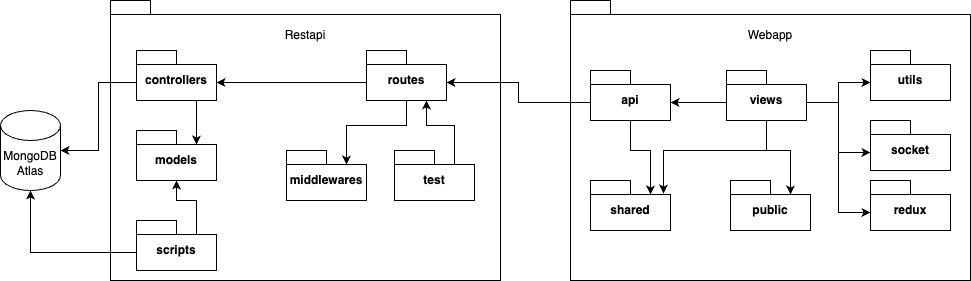
\includegraphics[width=0.8\linewidth]{figures/6-Analisis/6-Clases/6_5-vista_general-paquetes.png}
    \caption{Diagrama de Paquetes del Sistema}
    \label{fig:6_5_Diagrama-Paquetes}
\end{figure}

\subsection{Descripción de los Paquetes}
\subsubsection{restapi}
El paquete \textbf{restapi} contiene las clases que implementan la API REST del sistema y la lógica de negocio. Este paquete se divide en los siguientes subpaquetes:
\begin{itemize}
    \item \textbf{controllers}: contiene las clases que implementan los controladores de la API REST, se encargan de gestionar las peticiones HTTP y las respuestas. Se comunica con la base de datos.
    \item \textbf{models}: contiene las clases que implementan los modelos de datos del sistema.
    \item \textbf{routes}: contiene las clases que implementan las rutas de la API REST, se encargan de definir las rutas y los métodos HTTP asociados.
    \item \textbf{middlewares}: contiene las clases que implementan los middlewares de la API REST, se encargan de gestionar la autenticación y la autorización de los usuarios.
    \item \textbf{scripts}: contiene las clases que implementan los scripts de inicialización de la base de datos.
    \item \textbf{tests}: contiene las clases que implementan las pruebas unitarias de las clases de los otros subpaquetes.
\end{itemize}


\subsubsection{frontend}
El paquete \textbf{frontend} contiene los archivos que implementan la interfaz de usuario. Este paquete se divide en los siguientes subpaquetes:
\begin{itemize} 
    \item \textbf{src}: contiene los archivos que implementan la lógica de la interfaz de usuario.
    \begin{itemize}
        \item \textbf{api}: contiene los archivos que implementan la API del frontend, se encargan de gestionar las peticiones HTTP/HTTPS al backend.
        \item \textbf{views}: contiene los componentes que implementan las vistas de la interfaz de usuario. A su vez, se divide en los siguientes subpaquetes:
        \begin{itemize}
            \item \textbf{components}: contiene los archivos que implementan los componentes de la interfaz de usuario.
            \item \textbf{pages}: contiene las archivos que implementan las páginas de la interfaz de usuario.
        \end{itemize}
        \item \textbf{redux}: contiene las archivos que implementan los estados de Redux.
        \item \textbf{socket}: contiene las archivos que implementan la conexión con Socket.io.
        \item \textbf{shared}: contiene las archivos que implementan los tipos de datos compartidos entre las distintas partes de la interfaz de usuario.
        \item \textbf{utils}: contiene las archivos que implementan utilidades de la interfaz de usuario.
    \end{itemize}
    \item \textbf{public}: contiene los archivos estáticos de la interfaz de usuario.
    \item \textbf{tests}: contiene las clases que implementan las pruebas de la interfaz de usuario.
\end{itemize}

\subsection{Diagramas de Componentes}
En el estándar UML se define como componente: 
\begin{quote}
    \"Un Componente representa una parte modular de un sistema que encapsula su contenido y cuya manifestación es reemplazable dentro de su entorno.
[...]
Un Componente especifica un contrato formal de los servicios que proporciona a sus clientes y aquellos que requiere de otros Componentes o servicios en el sistema en términos de sus Interfaces proporcionadas y requeridas.
Un Componente es una unidad sustituible que puede ser reemplazada en tiempo de diseño o en tiempo de ejecución por un Componente que ofrece una funcionalidad equivalente basada en la compatibilidad de sus Interfaces. 
Siempre que el entorno sea totalmente compatible con las Interfaces proporcionadas y requeridas de un Componente, este podrá interactuar con dicho entorno."
\end{quote}

\begin{flushright}
    \cite[p. 209]{UMLomg2017}
\end{flushright}

En el contexto de este proyecto, un componente es una parte modular del sistema que encapsula su contenido y, que en un futuro, su funcionalidad podría ser ampliada o reemplazada por otra siempre que cumpla con las interfaces proporcionadas y requeridas.

\subsubsection{Diagrama de componentes del subsistema restapi}
A continuación, se presenta el diagrama de componentes del subsistema \textbf{restapi}. En este diagrama se muestran los componentes que forman parte del subsistema y las relaciones entre ellos.

    \begin{landscape}
    \begin{figure}[H]
        \hypertarget{fig:6_5_Diagrama-Componentes-restapi}{}
        \centering
        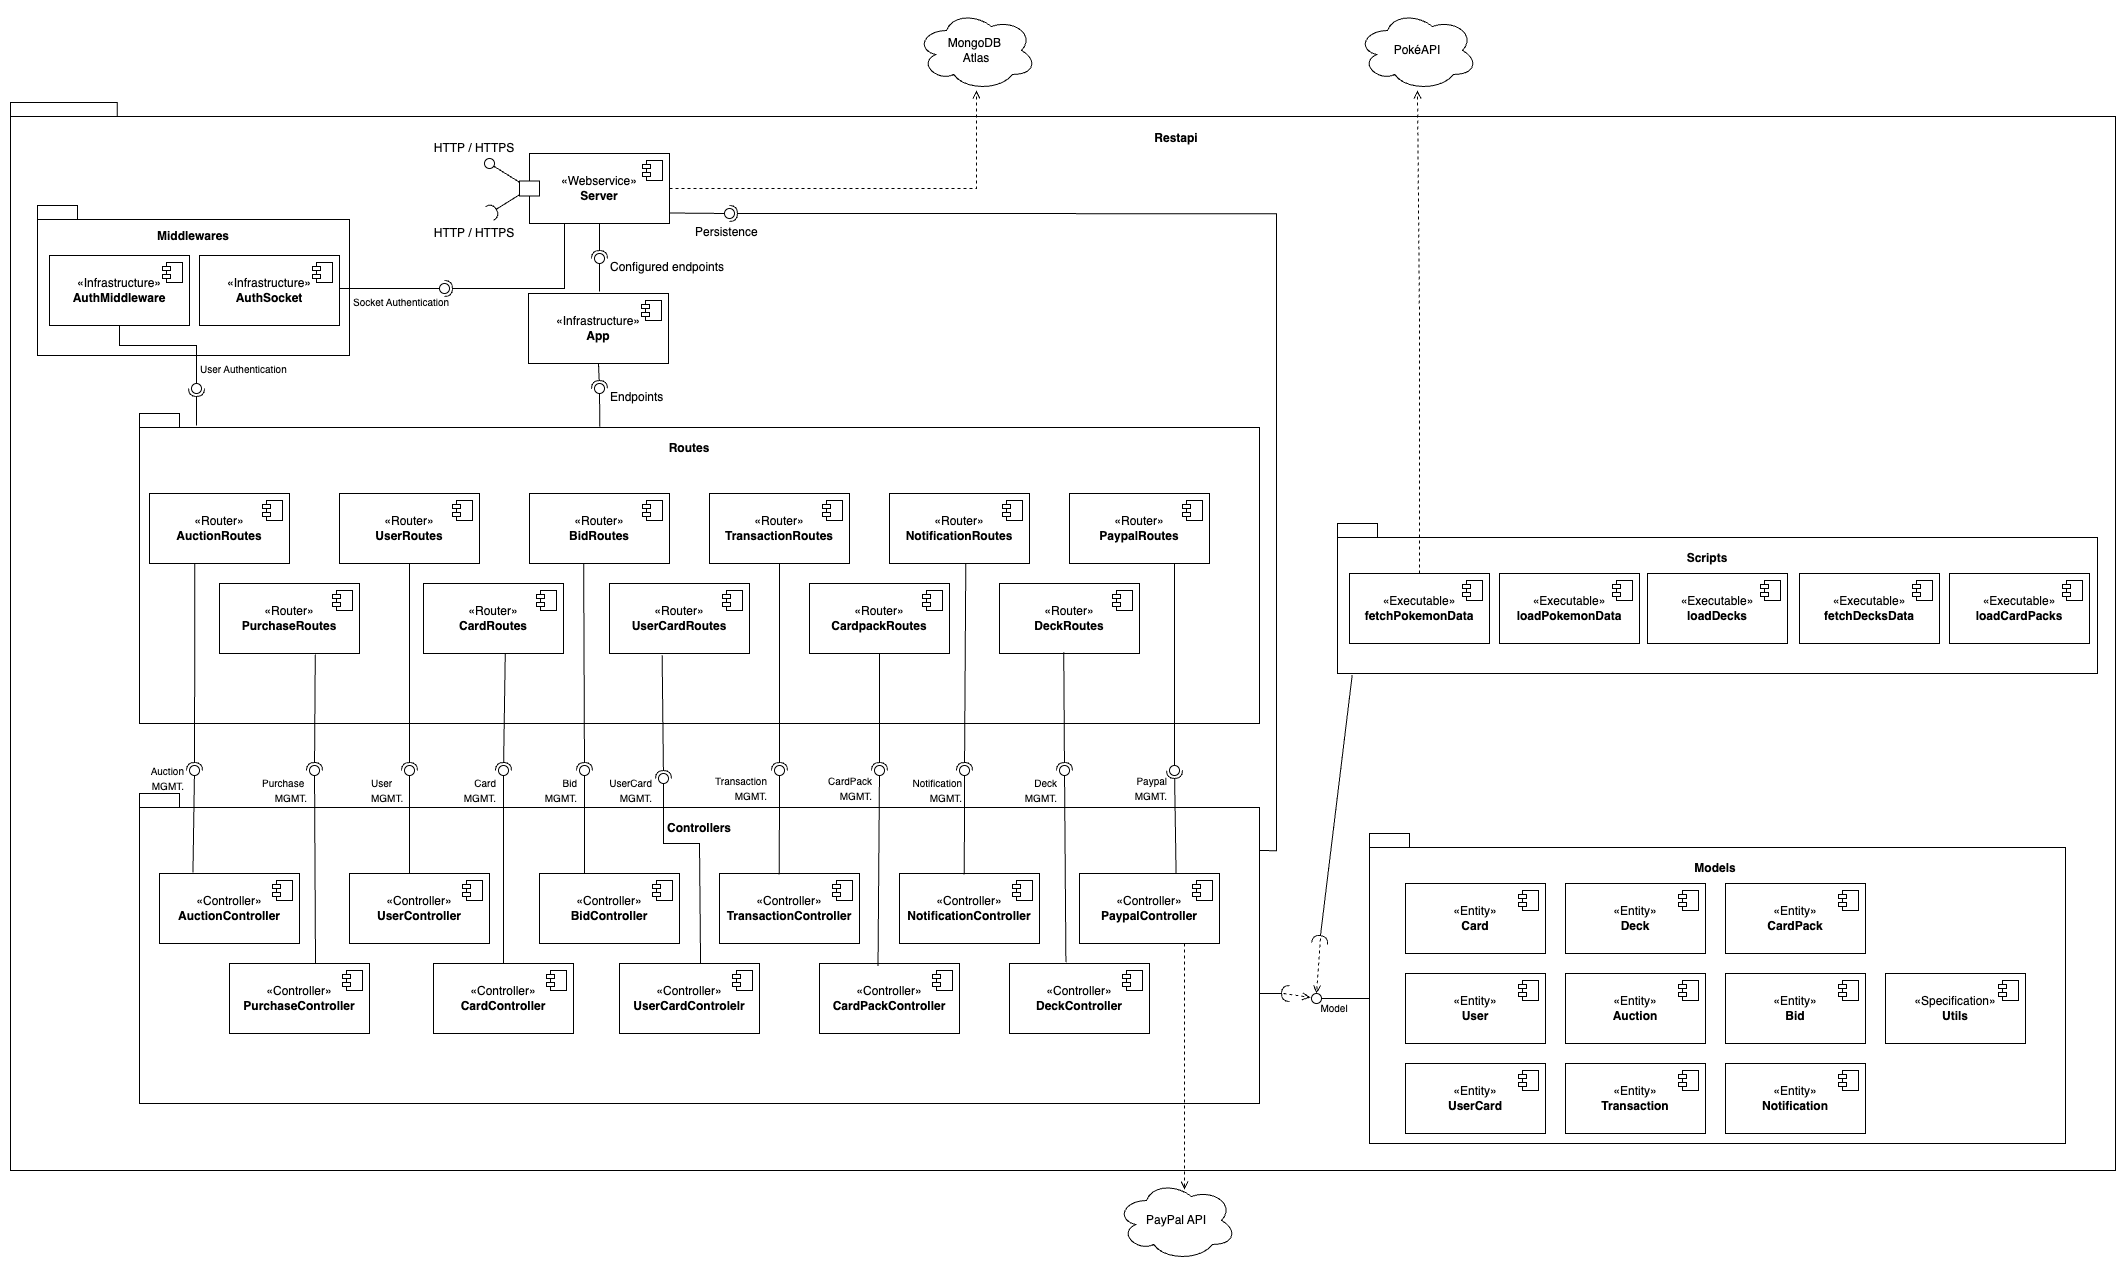
\includegraphics[width=1\linewidth]{figures/6-Analisis/6-Clases/6_5-Componentes-restapi.png}
        \caption{Diagrama de componentes del subsistema restapi}
        \label{fig:6_5_Diagrama-Componentes-restapi}
    \end{figure}
    \end{landscape}

\newpage

Por cada componente identificado en la \coloredUnderline{\hyperlink{fig:6_5_Diagrama-Componentes-restapi}{Figura \ref*{fig:6_5_Diagrama-Componentes-restapi}: \nameref*{fig:6_5_Diagrama-Componentes-restapi}}},
se ha creado una tabla con su descripción detallada, explicando su función específica dentro del sistema y las relaciones que mantiene con otros componentes.

\subsubsubsection{Descripción de componentes del subsistema restapi. \textit{Server} y \textit{App}}
%--- SERVER ---
\begin{longtable}{
    >{\columncolor{lightgreen!20}}p{4cm}
    p{12cm}
    }
    \caption{Descripción del componente:  Server} \label{table:descripcion_server} \\
    \toprule
    \rowcolor{darkgreen!50}
    \textbf{Componente} & \multicolumn{1}{>{\columncolor{darkgreen!50}\centering\arraybackslash}p{12cm}}{\textbf{SERVER}} \\
    \endfirsthead
    
    \multicolumn{2}{c}%
    {{ \tablename\ \thetable{} Descripción del componente:  Server -- continuación de la página anterior}} \\
    \toprule
    \rowcolor{darkgreen!50}
    \textbf{Componente} & \multicolumn{1}{>{\columncolor{darkgreen!50}\centering\arraybackslash}p{12cm}}{\textbf{SERVER}} \\
    \midrule
    \endhead
    
    \midrule
    \multicolumn{2}{r}{{Continúa en la siguiente página...}} \\ 
    \endfoot
    
    \bottomrule
    \endlastfoot
    
    \midrule
    Descripción & Este componente configura y gestiona los servidores HTTP y HTTPS, la conexión a MongoDB, y la gestión de conexiones de sockets mediante Socket.IO. También incluye la configuración de variables de entorno y el manejo de errores. \\
    \midrule
    Métodos & \begin{itemize}[nosep,leftmargin=*]
      \item \textbf{config()}: void, configura las variables de entorno.
      \item \textbf{createServers()}: void, crea y configura los servidores HTTP y HTTPS.
      \item \textbf{connectToDatabase()}: void, conecta a la base de datos MongoDB.
      \item \textbf{startServers()}: void, inicia los servidores HTTP y HTTPS.
      \item \textbf{setupSocketIO()}: void, configura el middleware de autenticación de sockets y maneja eventos de conexión y desconexión.
      \item \textbf{closeServer()}: Promise<void>, cierra los servidores HTTP, HTTPS y la conexión a la base de datos.
    \end{itemize} \\
    \midrule
    Interfaces requeridas & \begin{itemize}[nosep,leftmargin=*]
      \item \textbf{App}: Usa el componente App, que configura las rutas de la API REST.
      \item \textbf{AuthSocket}: Usa el middleware de autenticación de sockets.
      \item \textbf{HTTP/HTTPS}: Para la conexión a los servidores HTTP y HTTPS.
    \end{itemize} \\
    \midrule
    Interfaces proporcionadas & \begin{itemize}[nosep,leftmargin=*]
      \item \textbf{HTTP/HTTPS}: Proporciona la conexión a los servidores HTTP y HTTPS.
    \end{itemize} \\
\end{longtable}

%--- APP ---

\begin{longtable}{
    >{\columncolor{lightgreen!20}}p{4cm}
    p{12cm}
    }
    \caption{Descripción del componente:  App} \label{table:descripcion_app} \\
    \toprule
    \rowcolor{darkgreen!50}
    \textbf{Componente} & \multicolumn{1}{>{\columncolor{darkgreen!50}\centering\arraybackslash}p{12cm}}{\textbf{APP}} \\
    \endfirsthead
    
    \multicolumn{2}{c}%
    {{ \tablename\ \thetable{} Descripción del componente:  App -- continuación de la página anterior}} \\
    \toprule
    \rowcolor{darkgreen!50}
    \textbf{Componente} & \multicolumn{1}{>{\columncolor{darkgreen!50}\centering\arraybackslash}p{12cm}}{\textbf{APP}} \\
    \midrule
    \endhead
    
    \midrule
    \multicolumn{2}{r}{{Continúa en la siguiente página...}} \\ 
    \endfoot
    
    \bottomrule
    \endlastfoot
    
    \midrule
    Descripción & Este componente configura y gestiona las políticas CORS, las rutas de la API y el middleware para el manejo de errores. \\
    \midrule
    Métodos & \begin{itemize}[nosep,leftmargin=*]
      \item \textbf{use()}: void, permite configurar las rutas y los middlewares de la aplicación.
      \item \textbf{listen()}: void, inicia el servidor en el puerto especificado.
      \item \textbf{errorHandler()}: void, middleware para manejar errores en la aplicación.
    \end{itemize} \\
    \midrule
    Interfaces requeridas & \begin{itemize}[nosep,leftmargin=*]
      \item \textbf{Endpoints}: Utiliza todas las rutas de la API REST, definidas en el paquete \textit{routes}. Estas son:
        \begin{itemize}[nosep,leftmargin=*]
        \item \textbf{AuctionRouter}: Rutas que gestionan las subastas.
        \item \textbf{BidRouter}: Rutas que gestionan las pujas.
        \item \textbf{CardPackRouter}: Rutas que gestionan los sobres de cartas.
        \item \textbf{CardRouter}: Rutas que gestionan las cartas.
        \item \textbf{DeckRouter}: Rutas que gestionan los mazos de cartas.
        \item \textbf{NotificationRouter}: Rutas que gestionan las notificaciones.
        \item \textbf{PaypalRouter}: Rutas que gestionan las transacciones de PayPal.
        \item \textbf{PurchasesRouter}: Rutas que gestionan las compras.
        \item \textbf{TransactionRouter}: Rutas que gestionan las transacciones propias de la aplicación.
        \item \textbf{UserCardRouter}: Rutas que gestionan las cartas de usuario.
        \item \textbf{UserRouter}: Rutas que gestionan los usuarios.
        \end{itemize}
    \end{itemize} \\
    \midrule
    Interfaces proporcionadas & \begin{itemize}[nosep,leftmargin=*]
      \item \textbf{Configured endpoints}: Proporciona la aplicación de Express con las rutas y middlewares configurados.   
    \end{itemize} \\
\end{longtable}


%------------------------- PAQUETE MIDDLWARES -------------------------
\subsubsubsection{Descripción de componentes del subsistema restapi. Paquete \textit{middlewares}}\label{sec:descripcion_authmiddleware}
%--- AUTHMIDDLEWARE ---
\begin{longtable}{
    >{\columncolor{lightgreen!20}}p{4cm}
    p{12cm}
    }
    \caption{Descripción del componente:  AuthMiddleware} \label{table:descripcion_authmiddleware} \\
    \toprule
    \rowcolor{darkgreen!50}
    \textbf{Componente} & \multicolumn{1}{>{\columncolor{darkgreen!50}\centering\arraybackslash}p{12cm}}{\textbf{AUTHMIDDLEWARE}} \\
    \endfirsthead
    
    \multicolumn{2}{c}%
    {{ \tablename\ \thetable{} Descripción del componente:  AuthMiddleware -- continuación de la página anterior}} \\
    \toprule
    \rowcolor{darkgreen!50}
    \textbf{Componente} & \multicolumn{1}{>{\columncolor{darkgreen!50}\centering\arraybackslash}p{12cm}}{\textbf{AUTHMIDDLEWARE}} \\
    \midrule
    \endhead
    
    \midrule
    \multicolumn{2}{r}{{Continúa en la siguiente página...}} \\ 
    \endfoot
    
    \bottomrule
    \endlastfoot
    
    \midrule
    Descripción & Este componente proporciona middleware para la autenticación y autorización de usuarios mediante tokens JWT. Incluye la verificación de tokens y la verificación de roles de administrador. \\
    \midrule
    Métodos & \begin{itemize}[nosep,leftmargin=*]
      \item \textbf{auth(req: Request, res: Response, next: any)}: void, middleware para verificar la autenticidad del token JWT en las peticiones.
      \item \textbf{verifyAdmin(req: Request, res: Response, next: any)}: void, middleware para verificar que el usuario tiene rol de administrador.
    \end{itemize} \\
    \midrule
    Interfaces requeridas &  \\
    \midrule
    Interfaces proporcionadas & \begin{itemize}[nosep,leftmargin=*]
      \item \textbf{User Authentication}: Proporciona middleware para la autenticación de usuarios, verificando la validez del token JWT y, ofreciendo la posibilidad de verificar roles de administrador.
    \end{itemize} \\
    \end{longtable}

%--- AUTHSOCKET ---
\begin{longtable}{
    >{\columncolor{lightgreen!20}}p{4cm}
    p{12cm}
    }
    \caption{Descripción del componente:  AuthSocket} \label{table:descripcion_authsocket} \\
    \toprule
    \rowcolor{darkgreen!50}
    \textbf{Componente} & \multicolumn{1}{>{\columncolor{darkgreen!50}\centering\arraybackslash}p{12cm}}{\textbf{AUTHSOCKET}} \\
    \endfirsthead
    
    \multicolumn{2}{c}%
    {{ \tablename\ \thetable{} Descripción del componente:  AuthSocket -- continuación de la página anterior}} \\
    \toprule
    \rowcolor{darkgreen!50}
    \textbf{Componente} & \multicolumn{1}{>{\columncolor{darkgreen!50}\centering\arraybackslash}p{12cm}}{\textbf{AUTHSOCKET}} \\
    \midrule
    \endhead
    
    \midrule
    \multicolumn{2}{r}{{Continúa en la siguiente página...}} \\ 
    \endfoot
    
    \bottomrule
    \endlastfoot
    
    \midrule
    Descripción & Este componente proporciona el middleware para la autenticación de conexiones de sockets mediante tokens JWT. Verifica la validez y el formato del token proporcionado en el handshake de la conexión del socket. \\
    \midrule
    Métodos & \begin{itemize}[nosep,leftmargin=*]
      \item \textbf{authSocket(socket: Socket, next: (err?: Error) => void)}: void, middleware para verificar la autenticidad del token JWT en las conexiones de sockets.
    \end{itemize} \\
    \midrule
    Interfaces requeridas &  \\
    \midrule
    Interfaces proporcionadas & \begin{itemize}[nosep,leftmargin=*]
      \item \textbf{Socket Authentication}: Proporciona middleware para la autenticación de conexiones de sockets, verificando la validez del token JWT.
    \end{itemize} \\
    \end{longtable}

%------------------------- PAQUETE ROUTES -------------------------
\subsubsection{Descripción de componentes del subsistema restapi. Paquete \textit{routes}}
En el diagrama se muestra una relación de dependencia entre \textit{App} y los componentes del paquete \textit{routes}. 
En la práctica, cada componente del paquete \textit{routes} proporciona sus rutas a \textit{App} a través su propia instancia de \textit{Router} de Express. 
Se ha decidido simplificar la representación para facilitar la comprensión del diagrama, dado que todos los componentes del paquete \textit{routes} mantienen la misma relación con \textit{App}.

%--- AUCTIONROUTER ---
\begin{longtable}{
    >{\columncolor{lightgreen!20}}p{4cm}
    p{12cm}
    }
    \caption{Descripción del componente:  AuctionRouter} \label{table:descripcion_auctionrouter} \\
    \toprule
    \rowcolor{darkgreen!50}
    \textbf{Componente} & \multicolumn{1}{>{\columncolor{darkgreen!50}\centering\arraybackslash}p{12cm}}{\textbf{AUCTIONROUTER}} \\
    \endfirsthead
    
    \multicolumn{2}{c}%
    {{ \tablename\ \thetable{} Descripción del componente:  AuctionRouter -- continuación de la página anterior}} \\
    \toprule
    \rowcolor{darkgreen!50}
    \textbf{Componente} & \multicolumn{1}{>{\columncolor{darkgreen!50}\centering\arraybackslash}p{12cm}}{\textbf{AUCTIONROUTER}} \\
    \midrule
    \endhead
    
    \midrule
    \multicolumn{2}{r}{{Continúa en la siguiente página...}} \\ 
    \endfoot
    
    \bottomrule
    \endlastfoot
    
    \midrule
    Descripción & Este componente configura y gestiona las rutas relacionadas con las subastas en la aplicación Express. Incluye la autenticación mediante middleware y validaciones para las peticiones. \\
    \midrule
    Atributos & \begin{itemize}[nosep,leftmargin=*]
      \item \textbf{auctionRouter}: Router, instancia del enrutador de Express para las subastas.
    \end{itemize} \\
    \midrule
    Métodos & \begin{itemize}[nosep,leftmargin=*]
      \item \textbf{getAuctions(req: Request, res: Response)}: void, maneja la obtención de todas las subastas.
      \item \textbf{getAuction(req: Request, res: Response)}: void, maneja la obtención de una subasta por su ID.
      \item \textbf{getActiveAuctions(req: Request, res: Response)}: void, maneja la obtención de todas las subastas activas.
      \item \textbf{getActiveAuctionsByUser(req: Request, res: Response)}: void, maneja la obtención de todas las subastas activas de un usuario.
      \item \textbf{putUserCardUpForAuction(req: Request, res: Response)}: void, maneja la puesta en subasta de una carta de usuario.
      \item \textbf{withdrawnUserCardFromAuction(req: Request, res: Response)}: void, maneja la retirada de una carta de usuario de una subasta.
      \item \textbf{checkAllActiveAuctions(req: Request, res: Response)}: void, verifica todas las subastas activas y actualiza su estado si es necesario.
    \end{itemize} \\
    \midrule
    Interfaces requeridas &  \begin{itemize}[nosep,leftmargin=*]
      \item \textbf{User Authentication}: Middleware para la autenticación de usuarios.
      \item \textbf{Auction MGMT.}: Utiliza los métodos definidos en el controlador de subastas, \textit{AuctionController}.
    \end{itemize} \\
    \midrule
    Interfaces proporcionadas & \begin{itemize}[nosep,leftmargin=*]
      \item \textbf{Auction Router}: Proporciona las rutas para la gestión de subastas.
    \end{itemize} \\
    \end{longtable}

%--- BIDROUTER ---
\begin{longtable}{
    >{\columncolor{lightgreen!20}}p{4cm}
    p{12cm}
    }
    \caption{Descripción del componente:  BidRouter} \label{table:descripcion_bidrouter} \\
    \toprule
    \rowcolor{darkgreen!50}
    \textbf{Componente} & \multicolumn{1}{>{\columncolor{darkgreen!50}\centering\arraybackslash}p{12cm}}{\textbf{BIDROUTER}} \\
    \endfirsthead
    
    \multicolumn{2}{c}%
    {{ \tablename\ \thetable{} Descripción del componente:  BidRouter -- continuación de la página anterior}} \\
    \toprule
    \rowcolor{darkgreen!50}
    \textbf{Componente} & \multicolumn{1}{>{\columncolor{darkgreen!50}\centering\arraybackslash}p{12cm}}{\textbf{BIDROUTER}} \\
    \midrule
    \endhead
    
    \midrule
    \multicolumn{2}{r}{{Continúa en la siguiente página...}} \\ 
    \endfoot
    
    \bottomrule
    \endlastfoot
    
    \midrule
    Descripción & Este componente configura y gestiona las rutas relacionadas con las pujas en la aplicación Express. Incluye la autenticación mediante middleware y validaciones para las peticiones. \\
    \midrule
    Atributos & \begin{itemize}[nosep,leftmargin=*]
      \item \textbf{bidRouter}: Router, instancia del enrutador de Express para las pujas.
    \end{itemize} \\
    \midrule
    Métodos & \begin{itemize}[nosep,leftmargin=*]
      \item \textbf{getBidById(req: Request, res: Response)}: void, maneja la obtención de una puja por su ID.
      \item \textbf{createBid(req: Request, res: Response)}: void, maneja la creación de una nueva puja.
      \item \textbf{getActiveBidsByUser(req: Request, res: Response)}: void, maneja la obtención de todas las pujas activas de un usuario.
      \item \textbf{withdrawBid(req: Request, res: Response)}: void, maneja la retirada de una puja.
    \end{itemize} \\
    \midrule
    Relaciones & \begin{itemize}[nosep,leftmargin=*]
      \item \textbf{AuthMiddleware}: Middleware para la autenticación de usuarios.
      \item \textbf{BidController}: Importa y utiliza métodos del controlador de pujas.
    \end{itemize} \\
    \midrule
    Interfaces requeridas & \begin{itemize}[nosep,leftmargin=*]
      \item \textbf{User Authentication}: Middleware para la autenticación de usuarios.
      \item \textbf{Bid MGMT.}: Utiliza los métodos definidos en el controlador de pujas, \textit{BidController}.
    \end{itemize} \\
    \midrule
    Interfaces proporcionadas & \begin{itemize}[nosep,leftmargin=*]
      \item \textbf{Bid Router}: Proporciona las rutas para la gestión de pujas.
    \end{itemize} \\
    \end{longtable}

\subsubsubsection{Descripción del componente:  CardPackRouter} \label{sec:descripcion_cardpackrouter}
\begin{longtable}{
    >{\columncolor{lightgreen!20}}p{4cm}
    p{12cm}
    }
    \caption{Descripción del componente:  CardPackRouter} \label{table:descripcion_cardpackrouter} \\
    \toprule
    \rowcolor{darkgreen!50}
    \textbf{Componente} & \multicolumn{1}{>{\columncolor{darkgreen!50}\centering\arraybackslash}p{12cm}}{\textbf{CARDPACKROUTER}} \\
    \endfirsthead
    
    \multicolumn{2}{c}%
    {{ \tablename\ \thetable{} Descripción del componente:  CardPackRouter -- continuación de la página anterior}} \\
    \toprule
    \rowcolor{darkgreen!50}
    \textbf{Componente} & \multicolumn{1}{>{\columncolor{darkgreen!50}\centering\arraybackslash}p{12cm}}{\textbf{CARDPACKROUTER}} \\
    \midrule
    \endhead
    
    \midrule
    \multicolumn{2}{r}{{Continúa en la siguiente página...}} \\ 
    \endfoot
    
    \bottomrule
    \endlastfoot
    
    \midrule
    Descripción & Este componente configura y gestiona las rutas relacionadas con los sobres de cartas en la aplicación Express. Incluye la autenticación mediante middleware. \\
    \midrule
    Métodos & \begin{itemize}[nosep,leftmargin=*]
      \item \textbf{getCardPacks(req: Request, res: Response)}: void, maneja la obtención de todos los sobres de cartas.
    \end{itemize} \\
    \midrule
    Interfaces requeridas & \begin{itemize}[nosep,leftmargin=*]
      \item \textbf{User Authentication}: Middleware para la autenticación de usuarios.
      \item \textbf{CardPack MGMT.}: Utiliza los métodos definidos en el controlador de sobres de cartas, \textit{CardPackController}.
    \end{itemize} \\
    \midrule
    Interfaces proporcionadas & \begin{itemize}[nosep,leftmargin=*]
      \item \textbf{CardPack Router}: Proporciona las rutas para la gestión de sobres de cartas.
    \end{itemize} \\
    \end{longtable}


%--- CARDROUTER ---
\begin{longtable}{
    >{\columncolor{lightgreen!20}}p{4cm}
    p{12cm}
    }
    \caption{Descripción del componente:  CardRouter} \label{table:descripcion_cardrouter} \\
    \toprule
    \rowcolor{darkgreen!50}
    \textbf{Componente} & \multicolumn{1}{>{\columncolor{darkgreen!50}\centering\arraybackslash}p{12cm}}{\textbf{CARDROUTER}} \\
    \endfirsthead
    
    \multicolumn{2}{c}%
    {{ \tablename\ \thetable{} Descripción del componente:  CardRouter -- continuación de la página anterior}} \\
    \toprule
    \rowcolor{darkgreen!50}
    \textbf{Componente} & \multicolumn{1}{>{\columncolor{darkgreen!50}\centering\arraybackslash}p{12cm}}{\textbf{CARDROUTER}} \\
    \midrule
    \endhead
    
    \midrule
    \multicolumn{2}{r}{{Continúa en la siguiente página...}} \\ 
    \endfoot
    
    \bottomrule
    \endlastfoot
    
    \midrule
    Descripción & Esta clase configura y gestiona las rutas relacionadas con las cartas en la aplicación Express. Incluye la autenticación mediante middleware y validaciones para las peticiones. \\
    \midrule
    Métodos & \begin{itemize}[nosep,leftmargin=*]
      \item \textbf{getCard(req: Request, res: Response)}: void, maneja la obtención de una carta por su ID.
    \end{itemize} \\
    \midrule
    Interfaces requeridas  & \begin{itemize}[nosep,leftmargin=*]
      \item \textbf{User Authentication}: Middleware para la autenticación de usuarios.
      \item \textbf{Card MGMT.}: Utiliza los métodos definidos en el controlador de cartas, \textit{CardController}.
    \end{itemize} \\
    \midrule
    Interfaces proporcionadas & \begin{itemize}[nosep,leftmargin=*]
        \item \textbf{Card Router}: Proporciona las rutas para la gestión de cartas.
    \end{itemize} \\
    \end{longtable}

% --- NOTIFICATIONROUTER ---
\begin{longtable}{
    >{\columncolor{lightgreen!20}}p{4cm}
    p{12cm}
    }
    \caption{Descripción del componente:  NotificationRouter} \label{table:descripcion_notificationrouter} \\
    \toprule
    \rowcolor{darkgreen!50}
    \textbf{Componente} & \multicolumn{1}{>{\columncolor{darkgreen!50}\centering\arraybackslash}p{12cm}}{\textbf{NOTIFICATIONROUTER}} \\
    \endfirsthead
    
    \multicolumn{2}{c}%
    {{ \tablename\ \thetable{} Descripción del componente:  NotificationRouter -- continuación de la página anterior}} \\
    \toprule
    \rowcolor{darkgreen!50}
    \textbf{Componente} & \multicolumn{1}{>{\columncolor{darkgreen!50}\centering\arraybackslash}p{12cm}}{\textbf{NOTIFICATIONROUTER}} \\
    \midrule
    \endhead
    
    \midrule
    \multicolumn{2}{r}{{Continúa en la siguiente página...}} \\ 
    \endfoot
    
    \bottomrule
    \endlastfoot
    
    \midrule
    Descripción & Este componente configura y gestiona las rutas relacionadas con las notificaciones en la aplicación Express. Incluye la autenticación mediante middleware y validaciones para las peticiones. \\
    \midrule
    Atributos & \begin{itemize}[nosep,leftmargin=*]
      \item \textbf{notificationRouter}: Router, instancia del enrutador de Express para las notificaciones.
    \end{itemize} \\
    \midrule
    Métodos & \begin{itemize}[nosep,leftmargin=*]
      \item \textbf{getNotifications(req: Request, res: Response)}: void, maneja la obtención de todas las notificaciones de un usuario.
      \item \textbf{markAsRead(req: Request, res: Response)}: void, maneja el marcado de una notificación como leída.
      \item \textbf{markAllAsRead(req: Request, res: Response)}: void, maneja el marcado de todas las notificaciones de un usuario como leídas.
      \item \textbf{hasUnreadNotifications(req: Request, res: Response)}: void, verifica si un usuario tiene notificaciones no leídas.
    \end{itemize} \\
    \midrule
    Interfaces requeridas & \begin{itemize}[nosep,leftmargin=*]
      \item \textbf{User Authentication}: Middleware para la autenticación de usuarios.
      \item \textbf{Notification MGMT.}: Utiliza los métodos definidos en el controlador de notificaciones, \textit{NotificationController}.
    \end{itemize} \\
    \midrule
    Interfaces proporcionadas & \begin{itemize}[nosep,leftmargin=*]
        \item \textbf{Notification Router}: Proporciona las rutas para la gestión de notificaciones.
    \end{itemize} \\
    \end{longtable}

%--- PAYPALROUTER ---
\begin{longtable}{
    >{\columncolor{lightgreen!20}}p{4cm}
    p{12cm}
    }
    \caption{Descripción del componente:  PaypalRouter} \label{table:descripcion_paypalrouter} \\
    \toprule
    \rowcolor{darkgreen!50}
    \textbf{Componente} & \multicolumn{1}{>{\columncolor{darkgreen!50}\centering\arraybackslash}p{12cm}}{\textbf{PAYPALROUTER}} \\
    \endfirsthead
    
    \multicolumn{2}{c}%
    {{ \tablename\ \thetable{} Descripción del componente:  PaypalRouter -- continuación de la página anterior}} \\
    \toprule
    \rowcolor{darkgreen!50}
    \textbf{Componente} & \multicolumn{1}{>{\columncolor{darkgreen!50}\centering\arraybackslash}p{12cm}}{\textbf{PAYPALROUTER}} \\
    \midrule
    \endhead
    
    \midrule
    \multicolumn{2}{r}{{Continúa en la siguiente página...}} \\ 
    \endfoot
    
    \bottomrule
    \endlastfoot
    
    \midrule
    Descripción & Este componente configura y gestiona las rutas relacionadas con las órdenes de PayPal en la aplicación Express. Incluye validaciones para las peticiones y manejo de errores. \\
    \midrule
    Métodos & \begin{itemize}[nosep,leftmargin=*]
      \item \textbf{createOrder(req: Request, res: Response)}: void, maneja la creación de una nueva orden de PayPal.
      \item \textbf{updateOrder(req: Request, res: Response)}: void, maneja la actualización del saldo de un usuario después de completar un pago.
    \end{itemize} \\
    \midrule
    Interfaces requeridas & \begin{itemize}[nosep,leftmargin=*]
      \item \textbf{Paypal MGMT.}: Utiliza los métodos definidos en el controlador de PayPal, \textit{PaypalController}.
    \end{itemize} \\
    \midrule
    Interfaces proporcionadas & \begin{itemize}[nosep,leftmargin=*]
      \item \textbf{Paypal Router}: Proporciona las rutas para la gestión de órdenes de PayPal.
    \end{itemize} \\
    \end{longtable}

%------------------------- PAQUETE CONTROLLERS -------------------------



\subsubsection{Diagrama de componentes del subsistema webapp}
A continuación, se presenta el diagrama de componentes del subsistema \textbf{webapp}. En este diagrama se muestran los componentes que forman parte del subsistema.
Se han omitido las relaciones entre los componentes para simplificar el diagrama. Las relaciones entre los componentes se explicarán en la descripción de los componentes.
\begin{landscape}
    \begin{figure}[H]
        \hypertarget{fig:6_5_Diagrama-Componentes-webapp}{}
        \centering
        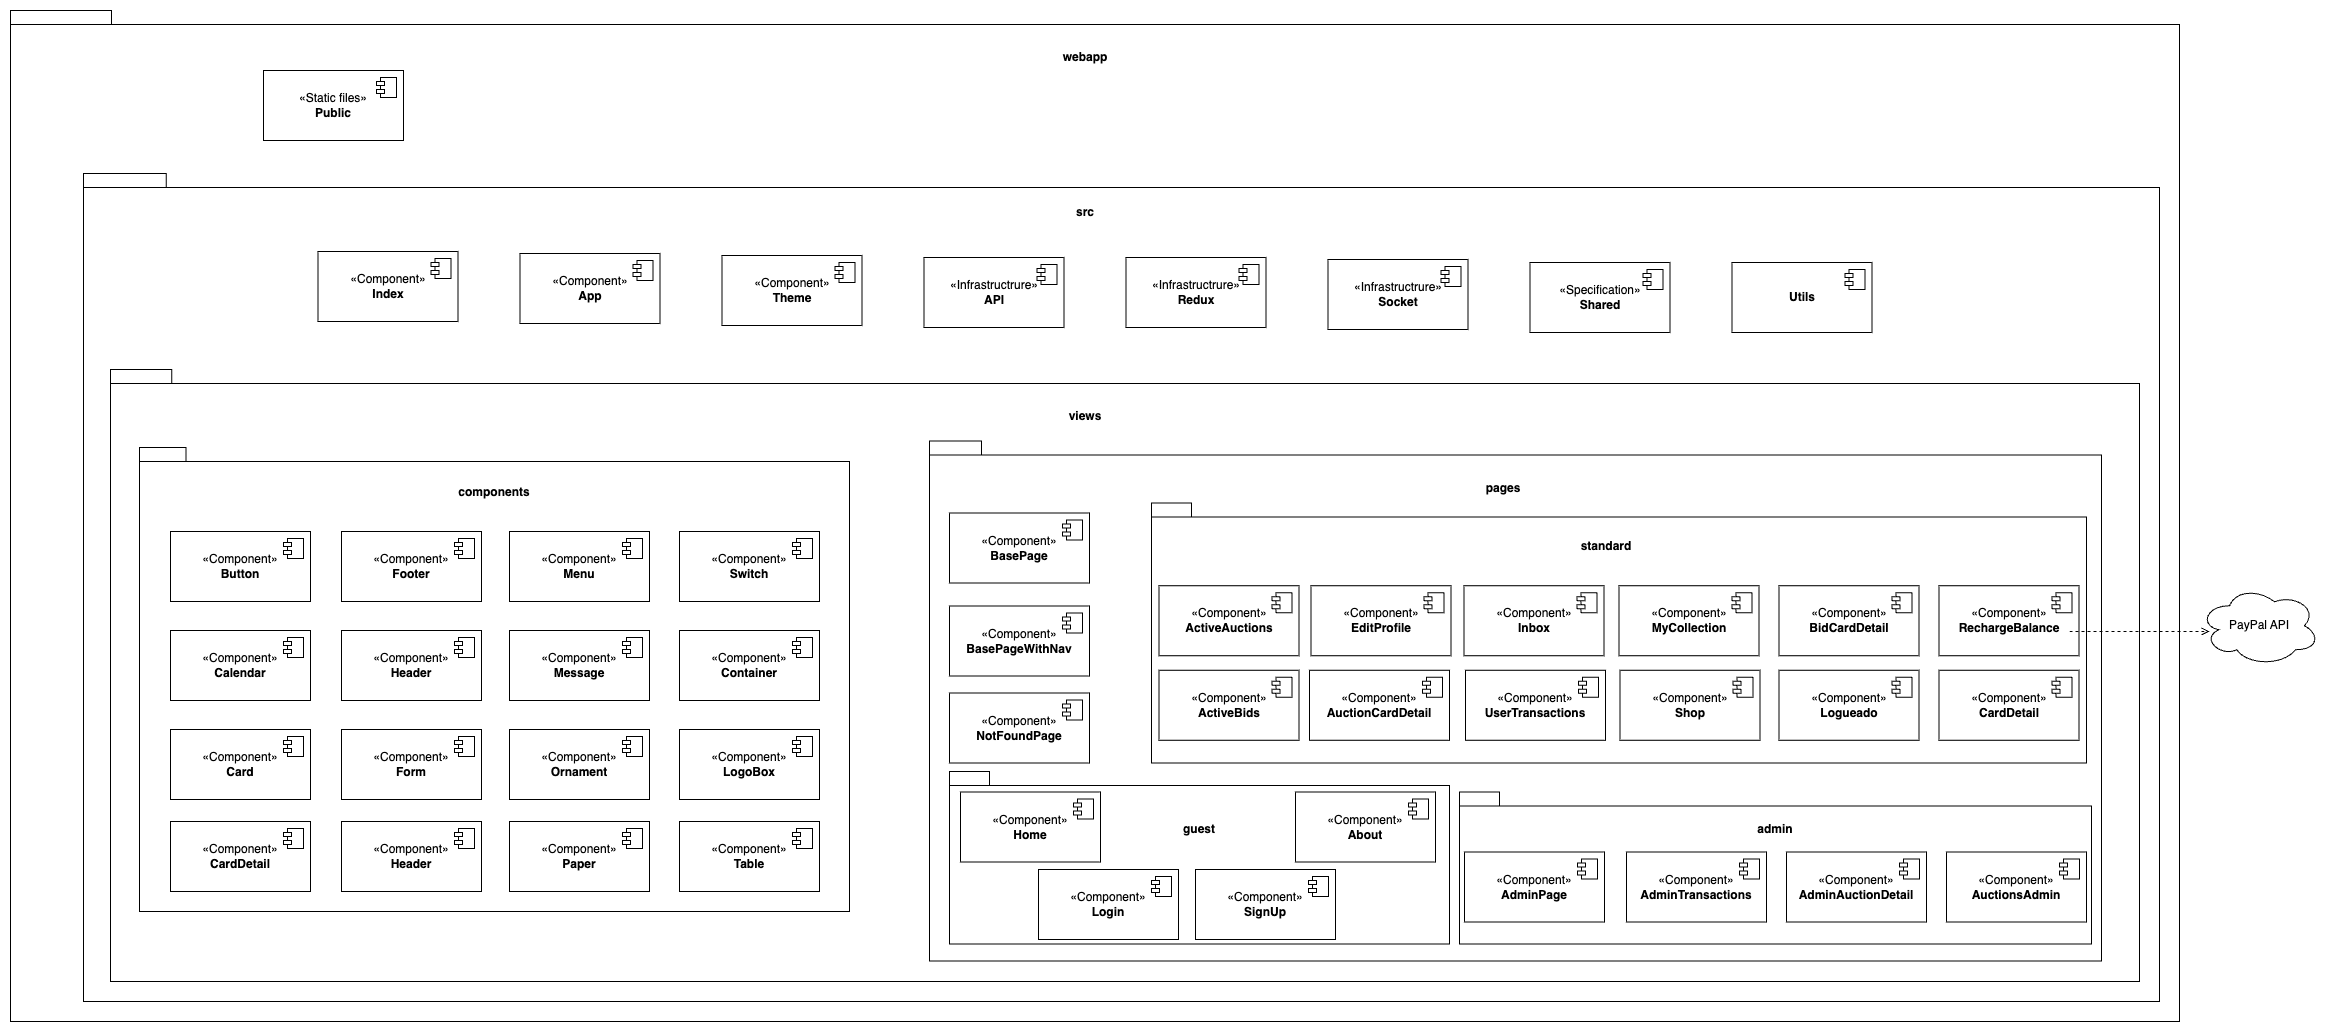
\includegraphics[width=1\linewidth]{figures/6-Analisis/6-Clases/6_5-Componentes-webapp.png}
        \caption{Diagrama de componentes del subsistema webapp}
        \label{fig:6_5_Diagrama-Componentes-webapp}
    \end{figure}
    \end{landscape}

\newpage

\subsubsubsection{Descripción de los Componentes del Subsistema webapp}
En este apartado se describirá la funcionalidad de los componentes del subsistema webapp. 
\begin{itemize}
    \item \textbf{Index}: Es el punto de entrada de la aplicación. Este componente se encarga del renderizado del componente \textit{App}.
    \item \textbf{App}: es el componente principal de la aplicación. Este componente define el diagrama de navegabilidad de la aplicación y se encarga de renderizar los componentes de la aplicación en función de la ruta actual. 
    Se relaciona, por lo tanto, con el paquete \textit{pages} y con el componente \textit{Theme} para definir el tema de la aplicación.
    \item \textbf{Theme}: es el componente que define el tema de la aplicación. Este componente se encarga de definir los colores y tipografías de la aplicación.
    \item \textbf{API}: es el componente que se encarga de realizar las peticiones a la API. Este componente se relaciona con el paquete \textit{shared} para definir los tipos de datos compartidos entre las distintas partes de la aplicación.
    \item \textbf{Redux}: es el componente que se encarga de gestionar el estado de la aplicación. Gestiona los siguientes estados:
    \begin{itemize}
        \item \textbf{user}: contiene la información del usuario autenticado.
        \item \textbf{notification}: estado para gestionar las visualizaciones de las notificaciones en tiempo real.
        \item \textbf{update}: estado para gestionar las actualizaciones de los datos de la aplicación.
    \end{itemize}
    \item \textbf{Socket}: es el componente que se encarga de gestionar la conexión con Socket.io. Concretamente se utiliza para que los usuarios puedan recibir notificaciones en tiempo real.
    \item \textbf{Shared}: es el componente que se encarga de definir los tipos de datos compartidos entre las distintas partes de la aplicación.
    \item \textbf{Utils}: es el componente que se encarga de definir utilidades de la aplicación. Contiene las siguientes utilidades:
    \begin{itemize}
        \item \textbf{cardData}: Colección de cartas de ejemplo para la aplicación. Se utiliza en un componente de la aplicación para mostrar cartas de ejemplo.
        \item \textbf{fieldsValidation}: utilidad para validar los campos de un formulario.
        \item \textbf{PrivateRoute}: componente que implementa una ruta privada de la aplicación. Verifica que un usuario esté autenticado antes de renderizar un componente.
        \item \textbf{RouteRedirector}: componente que implementa un redireccionador de rutas de la aplicación. Redirige a la ruta solicitada si el usuario cumple con el rol requerido, en caso contrario redirige a la ruta por defecto.
        \item \textbf{utils}: funciones de utilidad para la aplicación, como conversión de fechas y generación de mensajes.
    \end{itemize}
    \item \textbf{views}: contiene los componentes que implementan las vistas de la aplicación, y se divide en los siguientes subpaquetes:
    \begin{itemize}
        \item \textbf{components}: contiene los archivos que implementan los componentes de la aplicación. 
        Estos se usan para definir componentes más complejos que se reutilizan en distintas partes de la aplicación.
        \begin{itemize}
            \item \textbf{Button}: componente que implementa un botón de la aplicación. En este componente se definen los distintos tipos de botones que se utilizan en la aplicación.
            \item \textbf{Calendar}: componente que implementa un calendario de la aplicación.
            \item \textbf{Card}: componente que implementa una carta de la aplicación. 
            \item \textbf{CardDetail}: componente que implementa el modelo base de un detalle de carta.
            \item \textbf{Cardpack}: componente que implementa un sobre de cartas de la aplicación.
            \item \textbf{Container}: componente que implementa distintos tipos de contenedores de la aplicación.
            \item \textbf{Form}: componente que define los formularios de la aplicación.
            \item \textbf{Footer}: componente que implementa el pie de página de la aplicación.
            \item \textbf{Header}: componente que implementa la cabecera de la aplicación.
            \item \textbf{LogoBox}: componente que implementa el logotipo de la aplicación.
            \item \textbf{Menu}: componente que implementa los distintos menús de la aplicación.
            \item \textbf{Messages}: componente que implementa los distintos mensajes informativos de la aplicación.
            \item \textbf{Ornament}: componente que implementa distintos adornos de la aplicación.
            \item \textbf{Paper}: componente que implementa un contenedor con sombra, se utiliza para mostrar información en la aplicación.
            \item \textbf{Switch}: componente que implementa un interruptor de la aplicación. Concretamente, se utiliza para cambiar entre los modos claro y oscuro de la temática de la aplicación.
            \item \textbf{Table}: componente que implementa una tabla de la aplicación.
        \end{itemize}
        \item \textbf{pages}: contiene los archivos que implementan las páginas de la aplicación. Las páginas definen la estructura de las distintas vistas de la aplicación.
        Estas se crean utilizando los componentes definidos en el paquete \textit{components} junto con otros componentes de React.
        \begin{itemize}
            \item \textbf{BasePage}: página que implementa la estructura base de una página de la aplicación.
            \item \textbf{BasePageWithNav}: página que implementa la estructura base de una página de la aplicación con navegación.
            \item \textbf{NotFoundPage}: página que implementa la página de error 404.
            \item En el paquete \textit{guest} se encuentran las páginas que puede ver cualquier usuario:
            \begin{itemize}
                \item \textbf{Home}: página principal de la aplicación.
                \item \textbf{Login}: página de inicio de sesión.
                \item \textbf{SignUp}: página de registro de usuario.
                \item \textbf{About}: página de información sobre la aplicación.
            \end{itemize}
             \item En el paquete \textit{admin} se encuentran las páginas que puede ver un usuario con rol de administrador:
            \begin{itemize}
                \item \textbf{AdminPage}: página de administración de la aplicación.
                \item \textbf{AdminTransactions}: página de administración de usuarios.
                \item \textbf{AdminAuctionDetail}: página de administración de transacciones.
                \item \textbf{AuctionsAdmin}: página de administración de subastas.
            \end{itemize}
            \item En el paquete \textit{standard} se encuentran las páginas que puede ver un usuario autenticado con rol de usuario no administrador:
            \begin{itemize}
                \item \textbf{Logueado}: página de inicio del usuario autenticado.
                \item \textbf{EditProfile}: página de perfil del usuario autenticado.
                \item \textbf{CardDetail}: página de detalle de carta.
                \item \textbf{AuctionCardDetail}: página que muestra el detalle de una carta en subasta.
                \item \textbf{BidCardDetail}: página que muestra el detalle de una puja realizada a una determinada carta.
                \item \textbf{Shop}: página de tienda, en ella el usuario puede adquirir sobres de cartas.
                \item \textbf{ActiveAuctions}: página de subastas, en ella el usuario puede participar en subastas.
                \item \textbf{UserTransactions}: página de transacciones, en ella el usuario puede consultar las subastas realizadas.
                \item \textbf{InBox}: página de notificaciones, en ella el usuario puede consultar las notificaciones recibidas.
                \item \textbf{MyCollection}: página de colección, en ella el usuario puede consultar las cartas que posee.
                \item \textbf{RechargeBalance}: página de recarga de saldo, en ella el usuario puede recargar su saldo. Se comunica por HTTPS con la pasarela de pago, en este caso con la API de PayPal.
            \end{itemize}
        \end{itemize}
    \end{itemize}
\end{itemize}

% Nota adicional sobre los componentes
\bigskip
\textbf{Nota:} En el diagrama de componentes, una caja no necesariamente representa un único componente; puede representar múltiples componentes. 
Por ejemplo, en el caso del componente \textit{Button}, en la práctica se han implementado varios componentes que representan distintos tipos de botones de la aplicación.


\subsection{Diagrama de Despliegue}
En este apartado se describirá el proceso de despliegue de la aplicación, detallando los componentes y servicios necesarios para su correcto funcionamiento. 
Se presentará un diagrama de despliegue que ilustrará la arquitectura de la aplicación y la distribución de los componentes en el entorno de ejecución. 

Como se ha visto en la sección \coloredUnderline{\hyperlink{sec:identificacion-subsistemas-analisis}{\ref*{sec:identificacion-subsistemas-analisis}. \nameref*{sec:identificacion-subsistemas-analisis}}}, la aplicación se divide en dos subsistemas principales: \textbf{restapi} y \textbf{webapp}.
El subsistema \textbf{restapi} contiene las clases que implementan la API REST y la lógica de negocio, mientras que el subsistema \textbf{webapp} abarca la interfaz de usuario de la aplicación.
Estos dos subsistemas serán desplegados en una máquina virtual de Azure, utilizando contenedores Docker para facilitar su despliegue y escalabilidad.

Para desplegar la aplicación, se han seguido los siguientes pasos:
\begin{enumerate}
    \item \textbf{Crear la máquina virtual en Azure}: Se ha creado una máquina virtual en Azure con las características mencionadas anteriormente. 
    Además, es necesario crear un grupo de recursos y una red virtual para la máquina virtual. Las características de la máquina virtual son las siguientes:
    \begin{itemize}
        \item \textbf{Sistema Operativo}: Ubuntu 20.04 LTS.
        \item \textbf{Procesador}: 2 núcleos.
        \item \textbf{Memoria RAM}: 4 GB.
        \item \textbf{Discos de datos}: 4.
        \item \textbf{E/S máxima}: 1280 MB/s.
        \item \textbf{Almacenamiento local}: 8 GB.
        \item \textbf{Red}: IP pública y DNS asociado.
    \end{itemize}

    \item \textbf{Establecer un nombre de dominio}: Se ha asociado un nombre de dominio a la dirección IP pública de la máquina virtual para facilitar el acceso a la aplicación.

    \item \textbf{Contenedores Docker}: Se ha utilizado Docker para contenerizar la aplicación y facilitar su despliegue. 
    Para facilitar la tarea se ha configurado integración continua con GitHub Actions, de forma que cada vez que se realiza un \textit{pull-request} a la rama principal del repositorio, se construyen y despliegan los contenedores en la máquina virtual de Azure.
    Se han creado dos contenedores, uno para el subsistema \textbf{restapi} y otro para el subsistema \textbf{webapp}. Cada uno de estos expone uno o varios puertos diferentes para la comunicación con el exterior.

    \item \textbf{Configuración de Nginx como Proxy Inverso}: Se ha configurado Nginx como servidor web inverso para redirigir las peticiones a los contenedores correspondientes.
    Este paso es necesario para poder garantizar la seguridad de las comunicaciones con HTTPS. La configuración de Nginx incluye:
    \begin{itemize}
        \item \textbf{Obtención de certificado SSL}: Se ha utilizado Certbot para obtener un certificado SSL gratuito de Let's Encrypt y habilitar el protocolo HTTPS en la aplicación.
        \item \textbf{Redirección de Peticiones}: Configuración de Nginx para dirigir el tráfico HTTP y HTTPS a los contenedores adecuados.
    \end{itemize}

    \item \textbf{Configuración de la base de datos}: En la aplicación se usa como base de datos Mongo DB Atlas, que es una base de datos en la nube por lo que no es necesario configurarla en la máquina virtual, 
    pero sí es necesario configurar la conexión a la base de datos en la aplicación y permitir el acceso desde la dirección IP de la máquina virtual.

    \item \textbf{Docker Compose}: Se ha utilizado Docker Compose para orquestar los contenedores de la aplicación y facilitar su despliegue en la máquina virtual de Azure.
    Se ha creado un archivo \textit{docker-compose.yml} en la máquina virtual que define los servicios de la aplicación y sus configuraciones.

\end{enumerate}

Una vez realizados estos pasos, la aplicación estará desplegada y accesible a través del nombre de dominio asociado a la dirección IP pública de la máquina virtual.
Debido a los costos asociados al uso de la máquina virtual en Azure, se ha optado por mantener la máquina virtual apagada cuando no se está utilizando la aplicación.


En la \coloredUnderline{\hyperlink{fig:6_6_Diagrama-Despliegue}{Figura \ref*{fig:6_6_Diagrama-Despliegue}: \nameref*{fig:6_6_Diagrama-Despliegue}}} se muestra el diagrama de despliegue de la aplicación.
\begin{figure}[H]
    \hypertarget{fig:6_6_Diagrama-Despliegue}{}
    \centering
    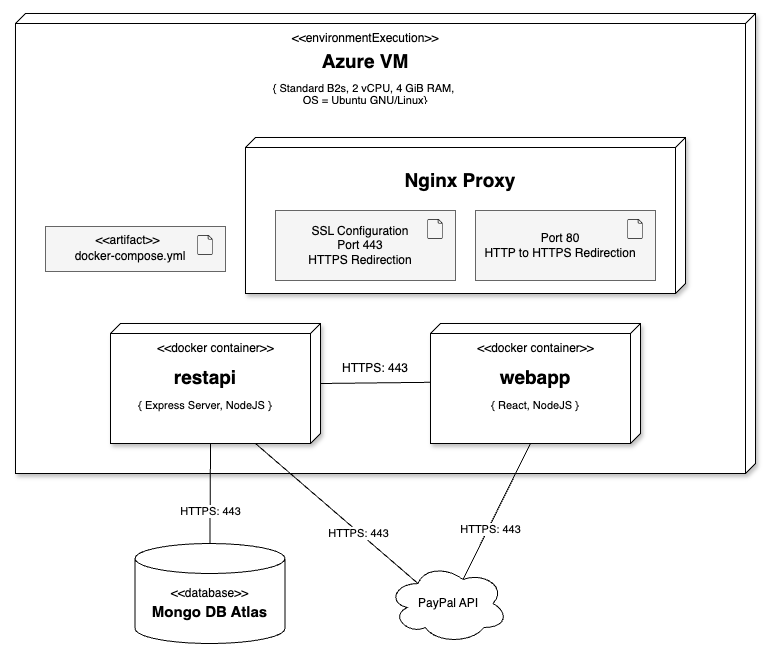
\includegraphics[width=0.8\linewidth]{figures/6-Analisis/6-Clases/6_5-Deployment.png}
    \caption{Diagrama de Despliegue de la Aplicación}
    \label{fig:6_6_Diagrama-Despliegue}
\end{figure}


\newpage
\section{DEFINICIÓN DE INTERFACES DE USUARIO}
% 6.6. Definición de interfaces de usuario + 7.4 Revisión de la Interfaz de Usuario
\subsection{Descripción de la Interfaz} 
Se ha desarrollado un conjunto de bocetos representativos para cada una de las interfaces principales, con el objetivo de facilitar la comprensión visual y estructural del sistema. 
Se ha decidido omitir la creación de bocetos para ciertas páginas del sistema, considerando que su simplicidad inherente no justifica una representación gráfica detallada, 
o debido a que su diseño es análogo al de otras interfaces previamente especificadas. 

\subsubsection{Página de Inicio}
La página de inicio es la primera página que se muestra al usuario al acceder al sistema.
Esta página se muestra cuando el usuario no ha iniciado sesión, y le permite acceder a las siguientes funcionalidades:
\begin{itemize}
    \item Iniciar sesión.
    \item Registrarse.
    \item Consultar información pública sobre el sistema (Enlaces del pie de página)
\end{itemize}

En la figura \ref{fig:p_home} se muestra el boceto de la página de inicio.

\begin{figure}[H]
    \centering
    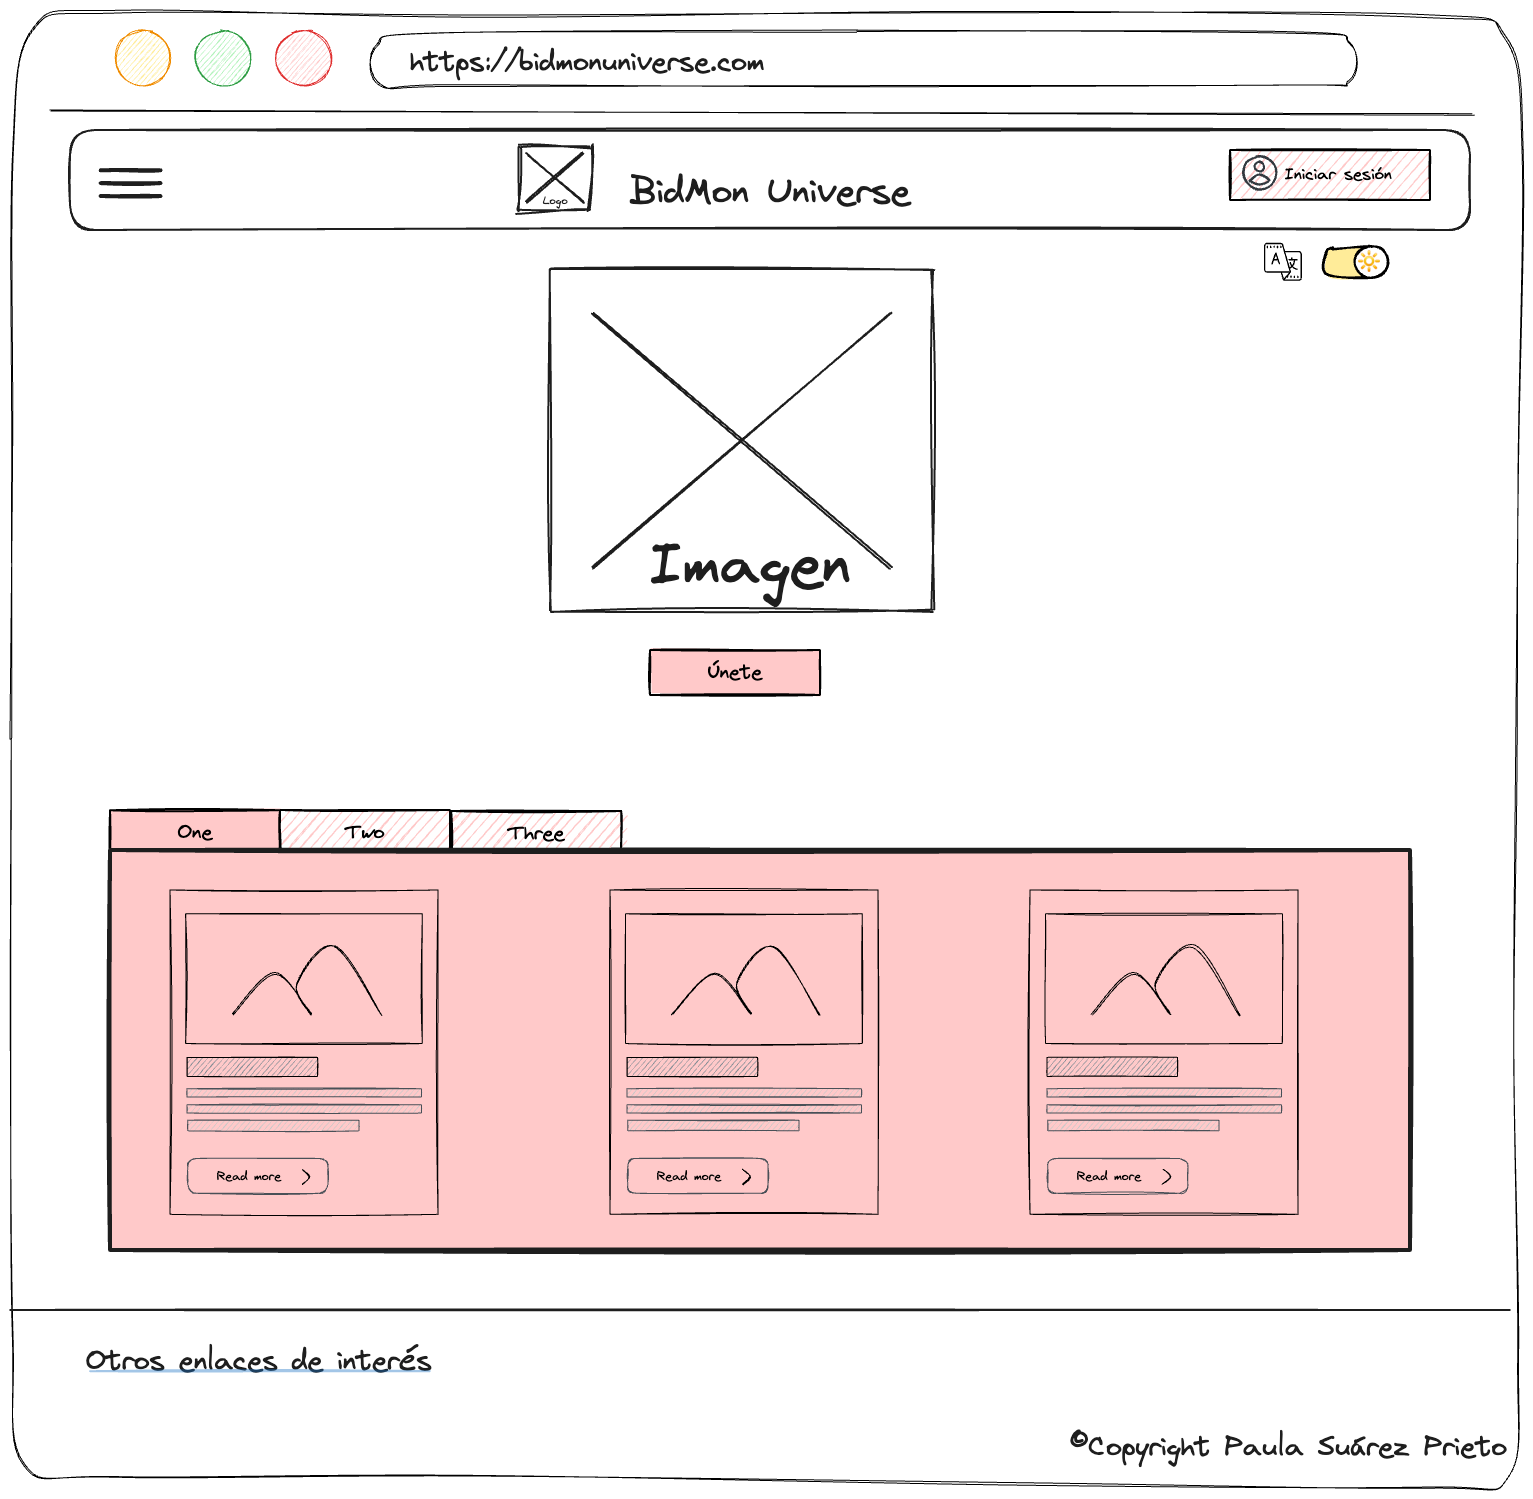
\includegraphics[width=0.8\textwidth]{figures/6-Analisis/6-Interfaz/prototipos/home.png}
    \caption{Boceto de la página de inicio}
    \label{fig:p_home}
\end{figure}

\subsubsection{Página de Inicio de Sesión}
La página de inicio de sesión muestra un formulario que permite al usuario ingresar sus credenciales para acceder al sistema o recuperar su contraseña.
En la figura \ref{fig:p_login} se muestra el boceto de la página de inicio de sesión.
En caso de que el usuario introduzca credenciales incorrectas, se mostrará un mensaje de error y se resaltarán los campos correspondientes.

\begin{figure}[H]
    \centering
    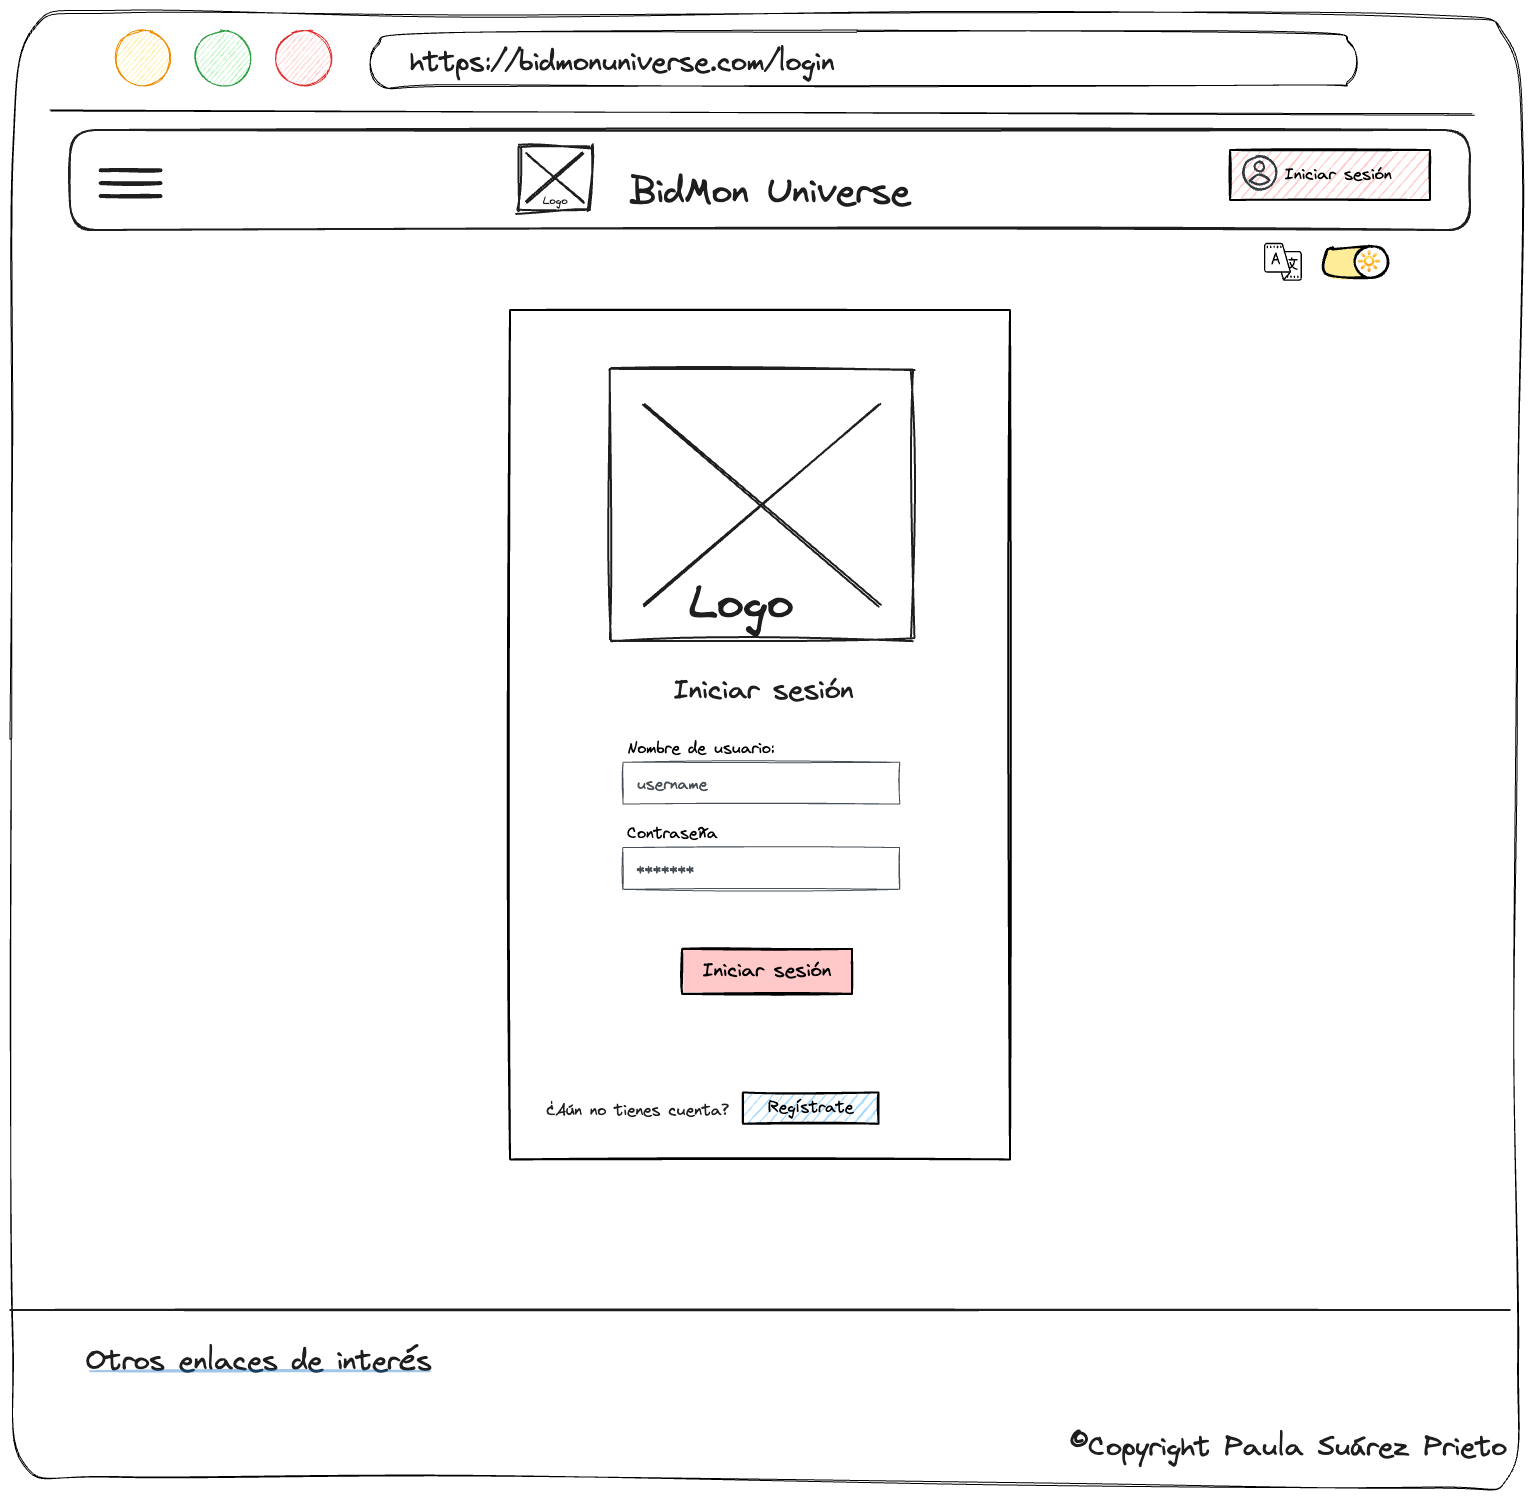
\includegraphics[width=0.8\textwidth]{figures/6-Analisis/6-Interfaz/prototipos/login.png}
    \caption{Boceto de la página de inicio de sesión}
    \label{fig:p_login}
\end{figure}

\subsubsection{Página de Registro}
La página de registro muestra un formulario que permite al usuario crear una cuenta en el sistema o iniciar sesión si ya tiene una cuenta.
En la figura \ref{fig:p_signup} se muestra el boceto de la página de registro.

En caso de que los campos del formulario no cumplan con las restricciones especificadas, se mostrará un mensaje de error y se resaltarán los campos correspondientes.

\begin{figure}[H]
    \centering
    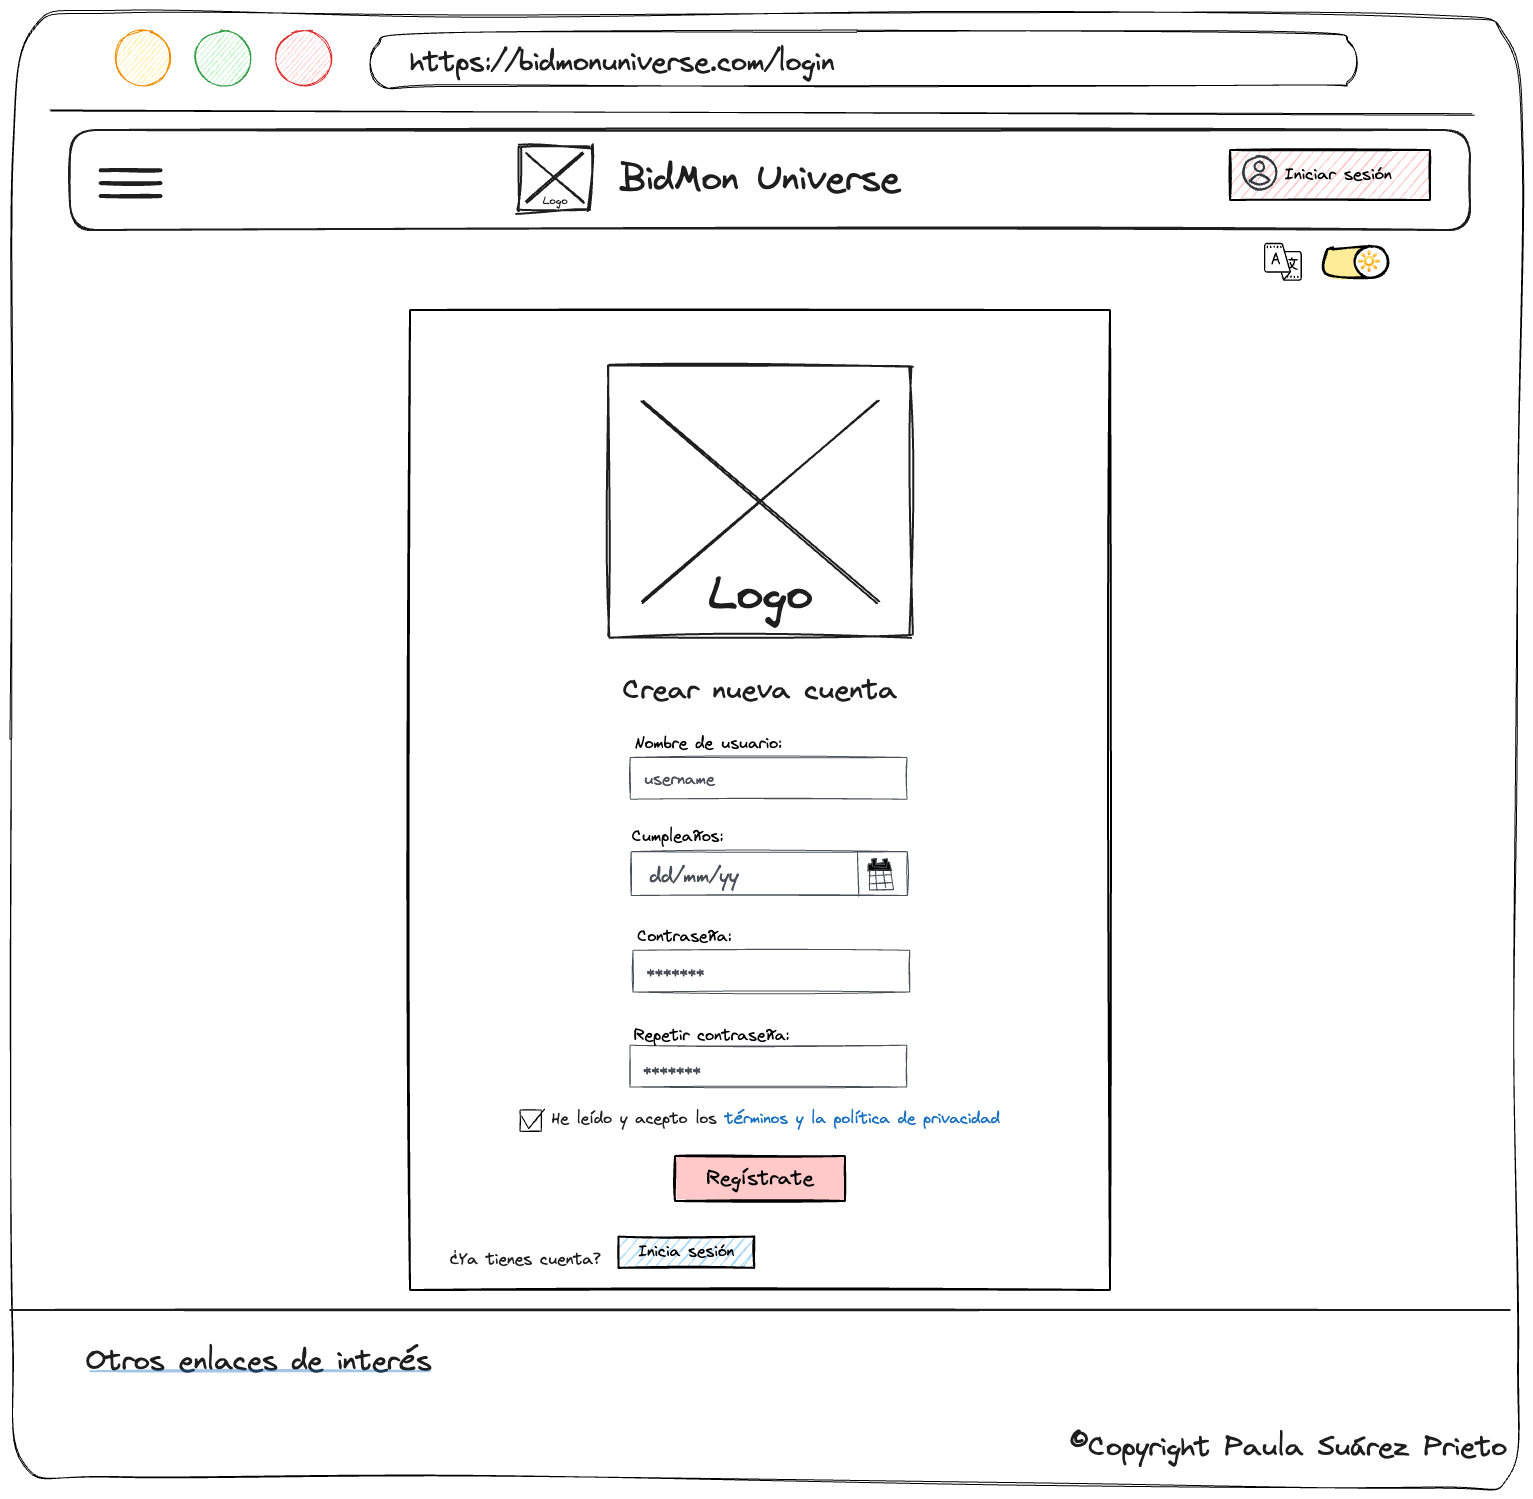
\includegraphics[width=0.8\textwidth]{figures/6-Analisis/6-Interfaz/prototipos/signup.png}
    \caption{Boceto de la página de registro}
    \label{fig:p_signup}
\end{figure}

\subsubsection{Página inicial de usuario}
Una vez que el usuario ha iniciado sesión en la plataforma, se le redirige a la página inicial de usuario.
Las páginas a las que tiene acceso un usuario autenticado muestran siempre como cabecera de la página un menú general de navegación que le permite acceder a las diferentes secciones del sistema,
el saldo de su cuenta y un menú de usuario que le permite acceder a su perfil y cerrar sesión.
La página inicial de usuario muestra un resumen de la información más relevante para el usuario:
\begin{itemize}
    \item Menú de acceso rápido a las secciones principales del sistema.
    \item Muestra las cartas más recientes de su colección con la posibilidad de acceder a la colección completa.
    \item Muestra las subastas activas iniciadas por el usuario más recientes con la posibilidad de acceder a las subastas completas.
    \item Muestra las pujas activas más recientes realizadas por el usuario con la posibilidad de acceder a las pujas completas.
\end{itemize}

En la figura \ref{fig:p_user_home} se muestra el boceto de la página inicial de usuario.

\begin{figure}[H]
    \centering
    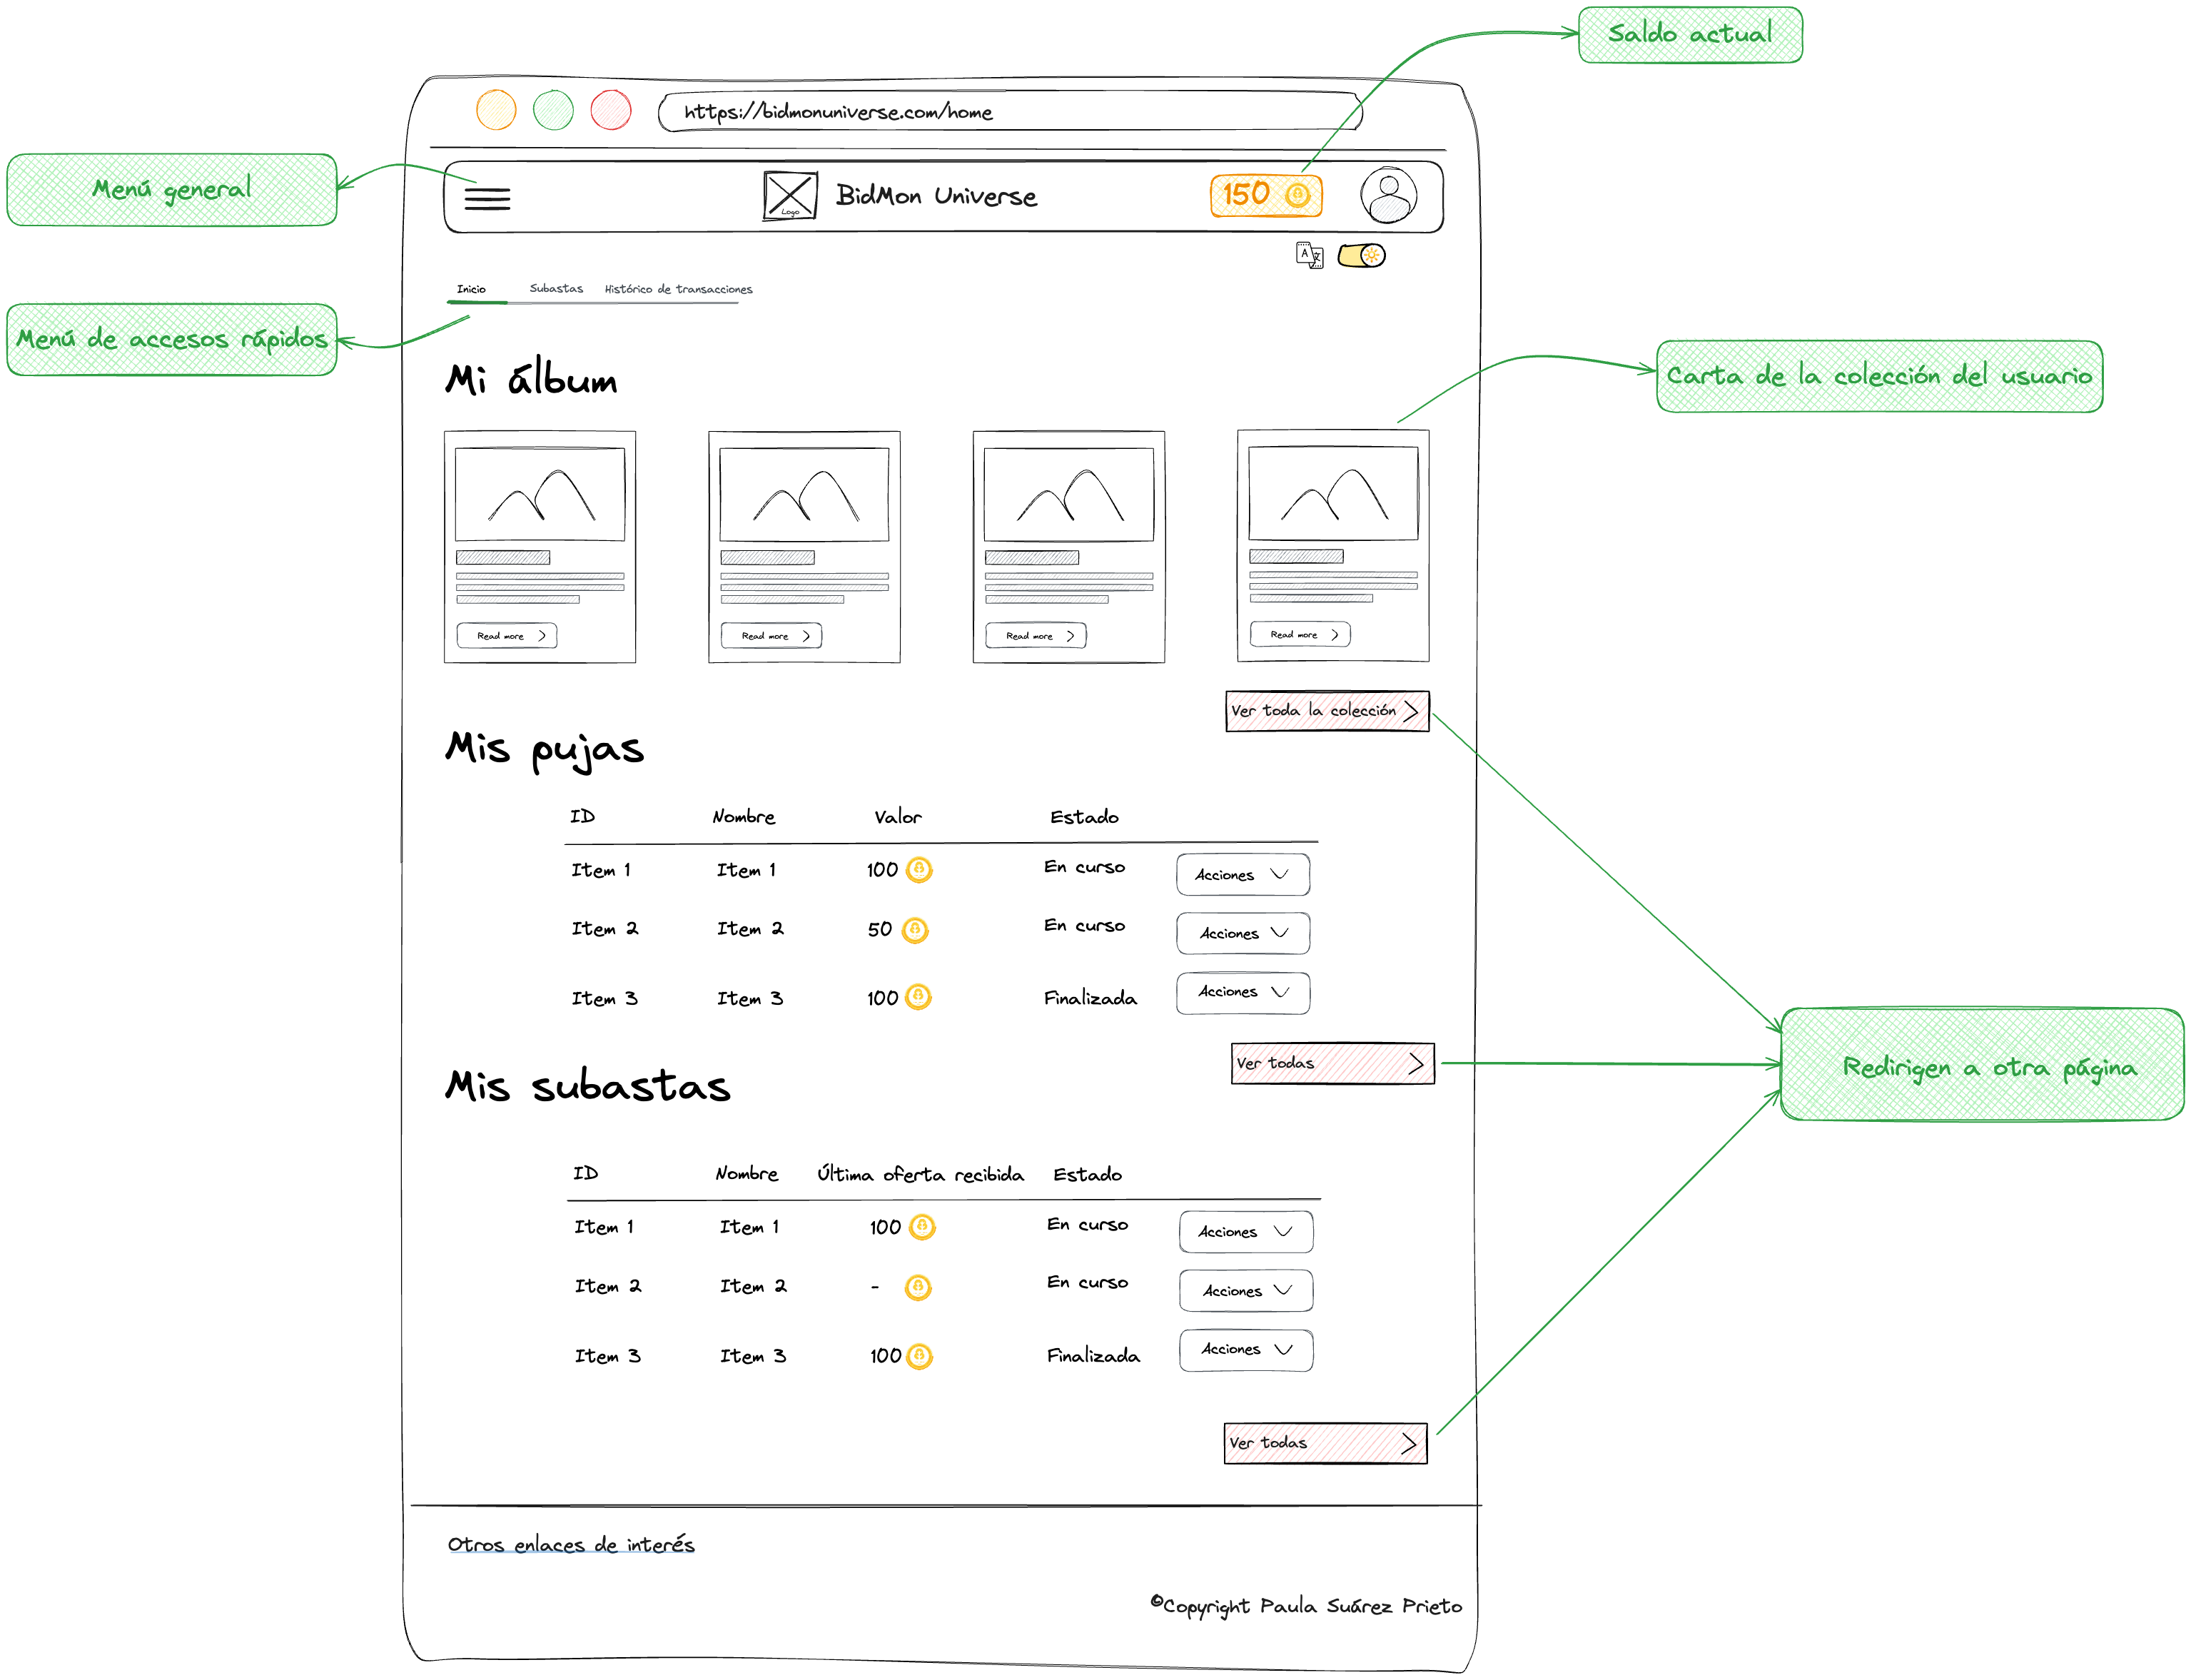
\includegraphics[width=1\textwidth]{figures/6-Analisis/6-Interfaz/prototipos/home-logueada.png}
    \caption{Boceto de la página inicial de usuario}
    \label{fig:p_user_home}
\end{figure}

\subsubsection{Página de Colección}
La página de colección muestra una lista de las cartas que el usuario ha añadido a su colección.
El usuario puede hacer clic en una carta para ver más detalles sobre ella.
En la figura \ref{fig:p_collection} se muestra el boceto de la página de colección.
\begin{figure}[H]
    \centering
    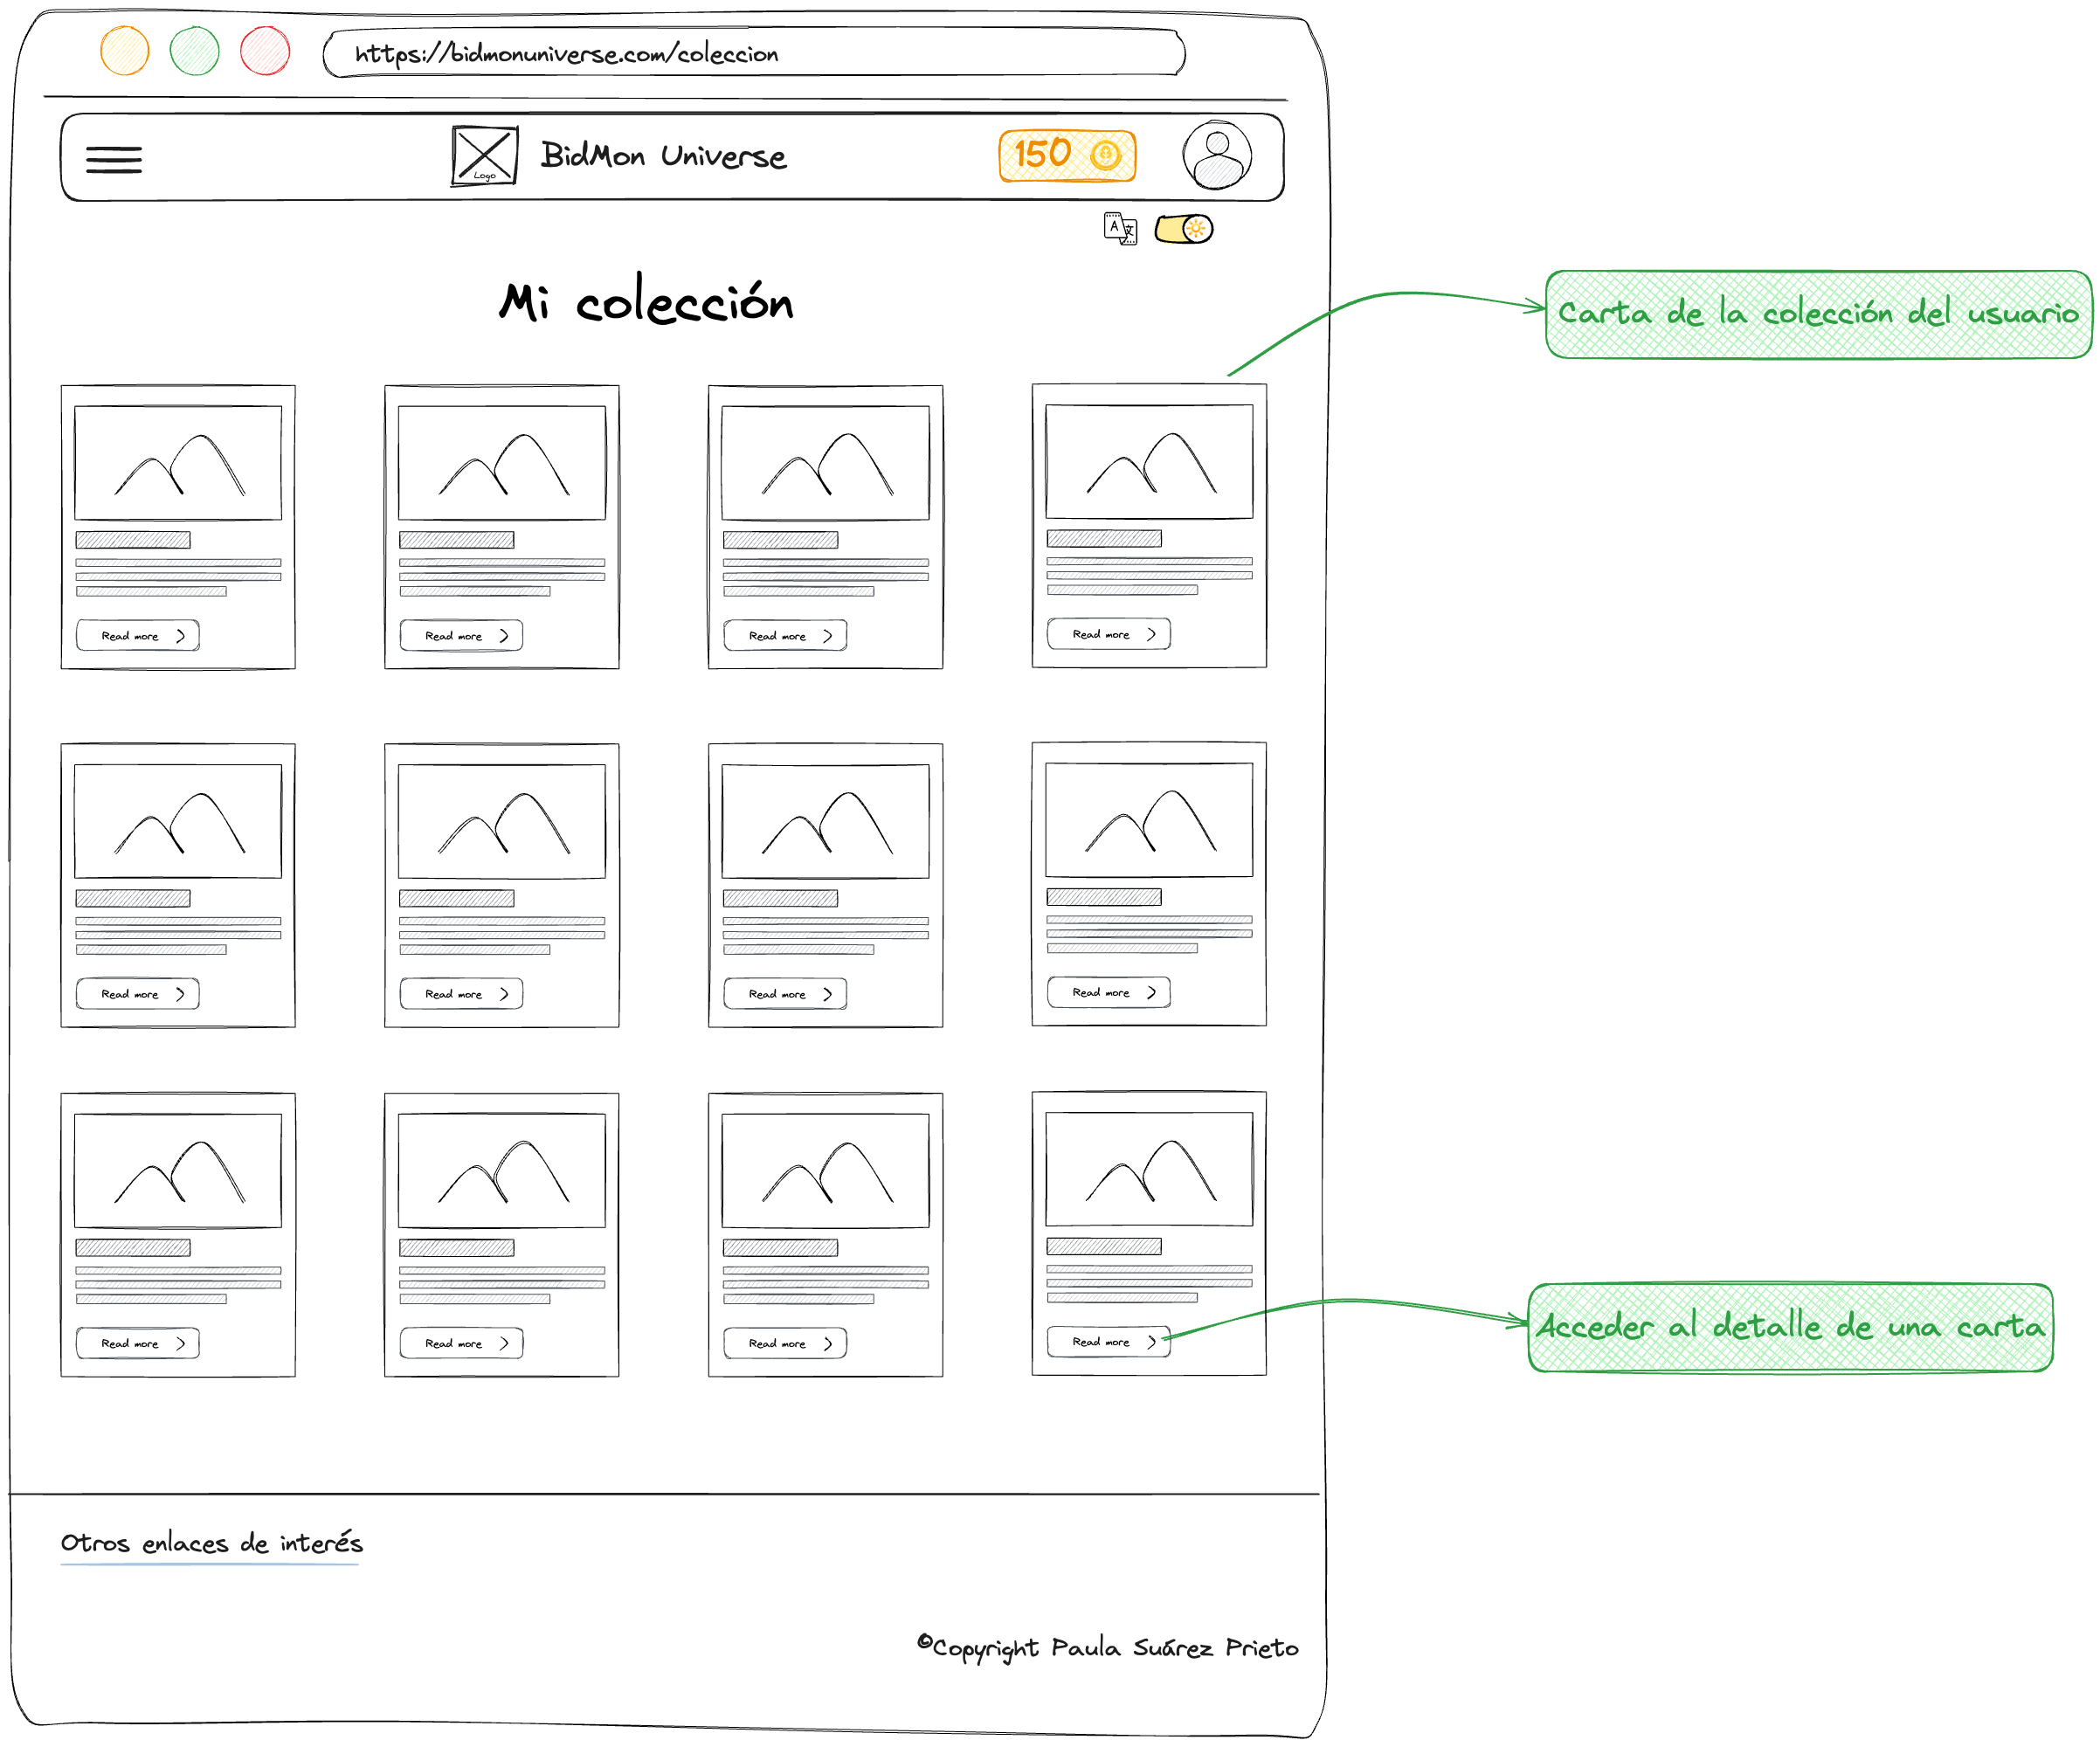
\includegraphics[width=0.9\textwidth]{figures/6-Analisis/6-Interfaz/prototipos/coleccion.png}
    \caption{Boceto de la página de colección}
    \label{fig:p_collection}
\end{figure}

\subsubsection{Página de Detalles de Carta}
La página de detalles de carta muestra información detallada sobre una carta específica. Permite al usuario ver la imagen de la carta, los datos de la carta, 
las transacciones de esta y la posibilidad de marcar la carta como destacada o subastarla.
En la figura \ref{fig:p_card_details} se muestra el boceto de la página de detalles de carta.
\begin{figure}[H]
    \centering
    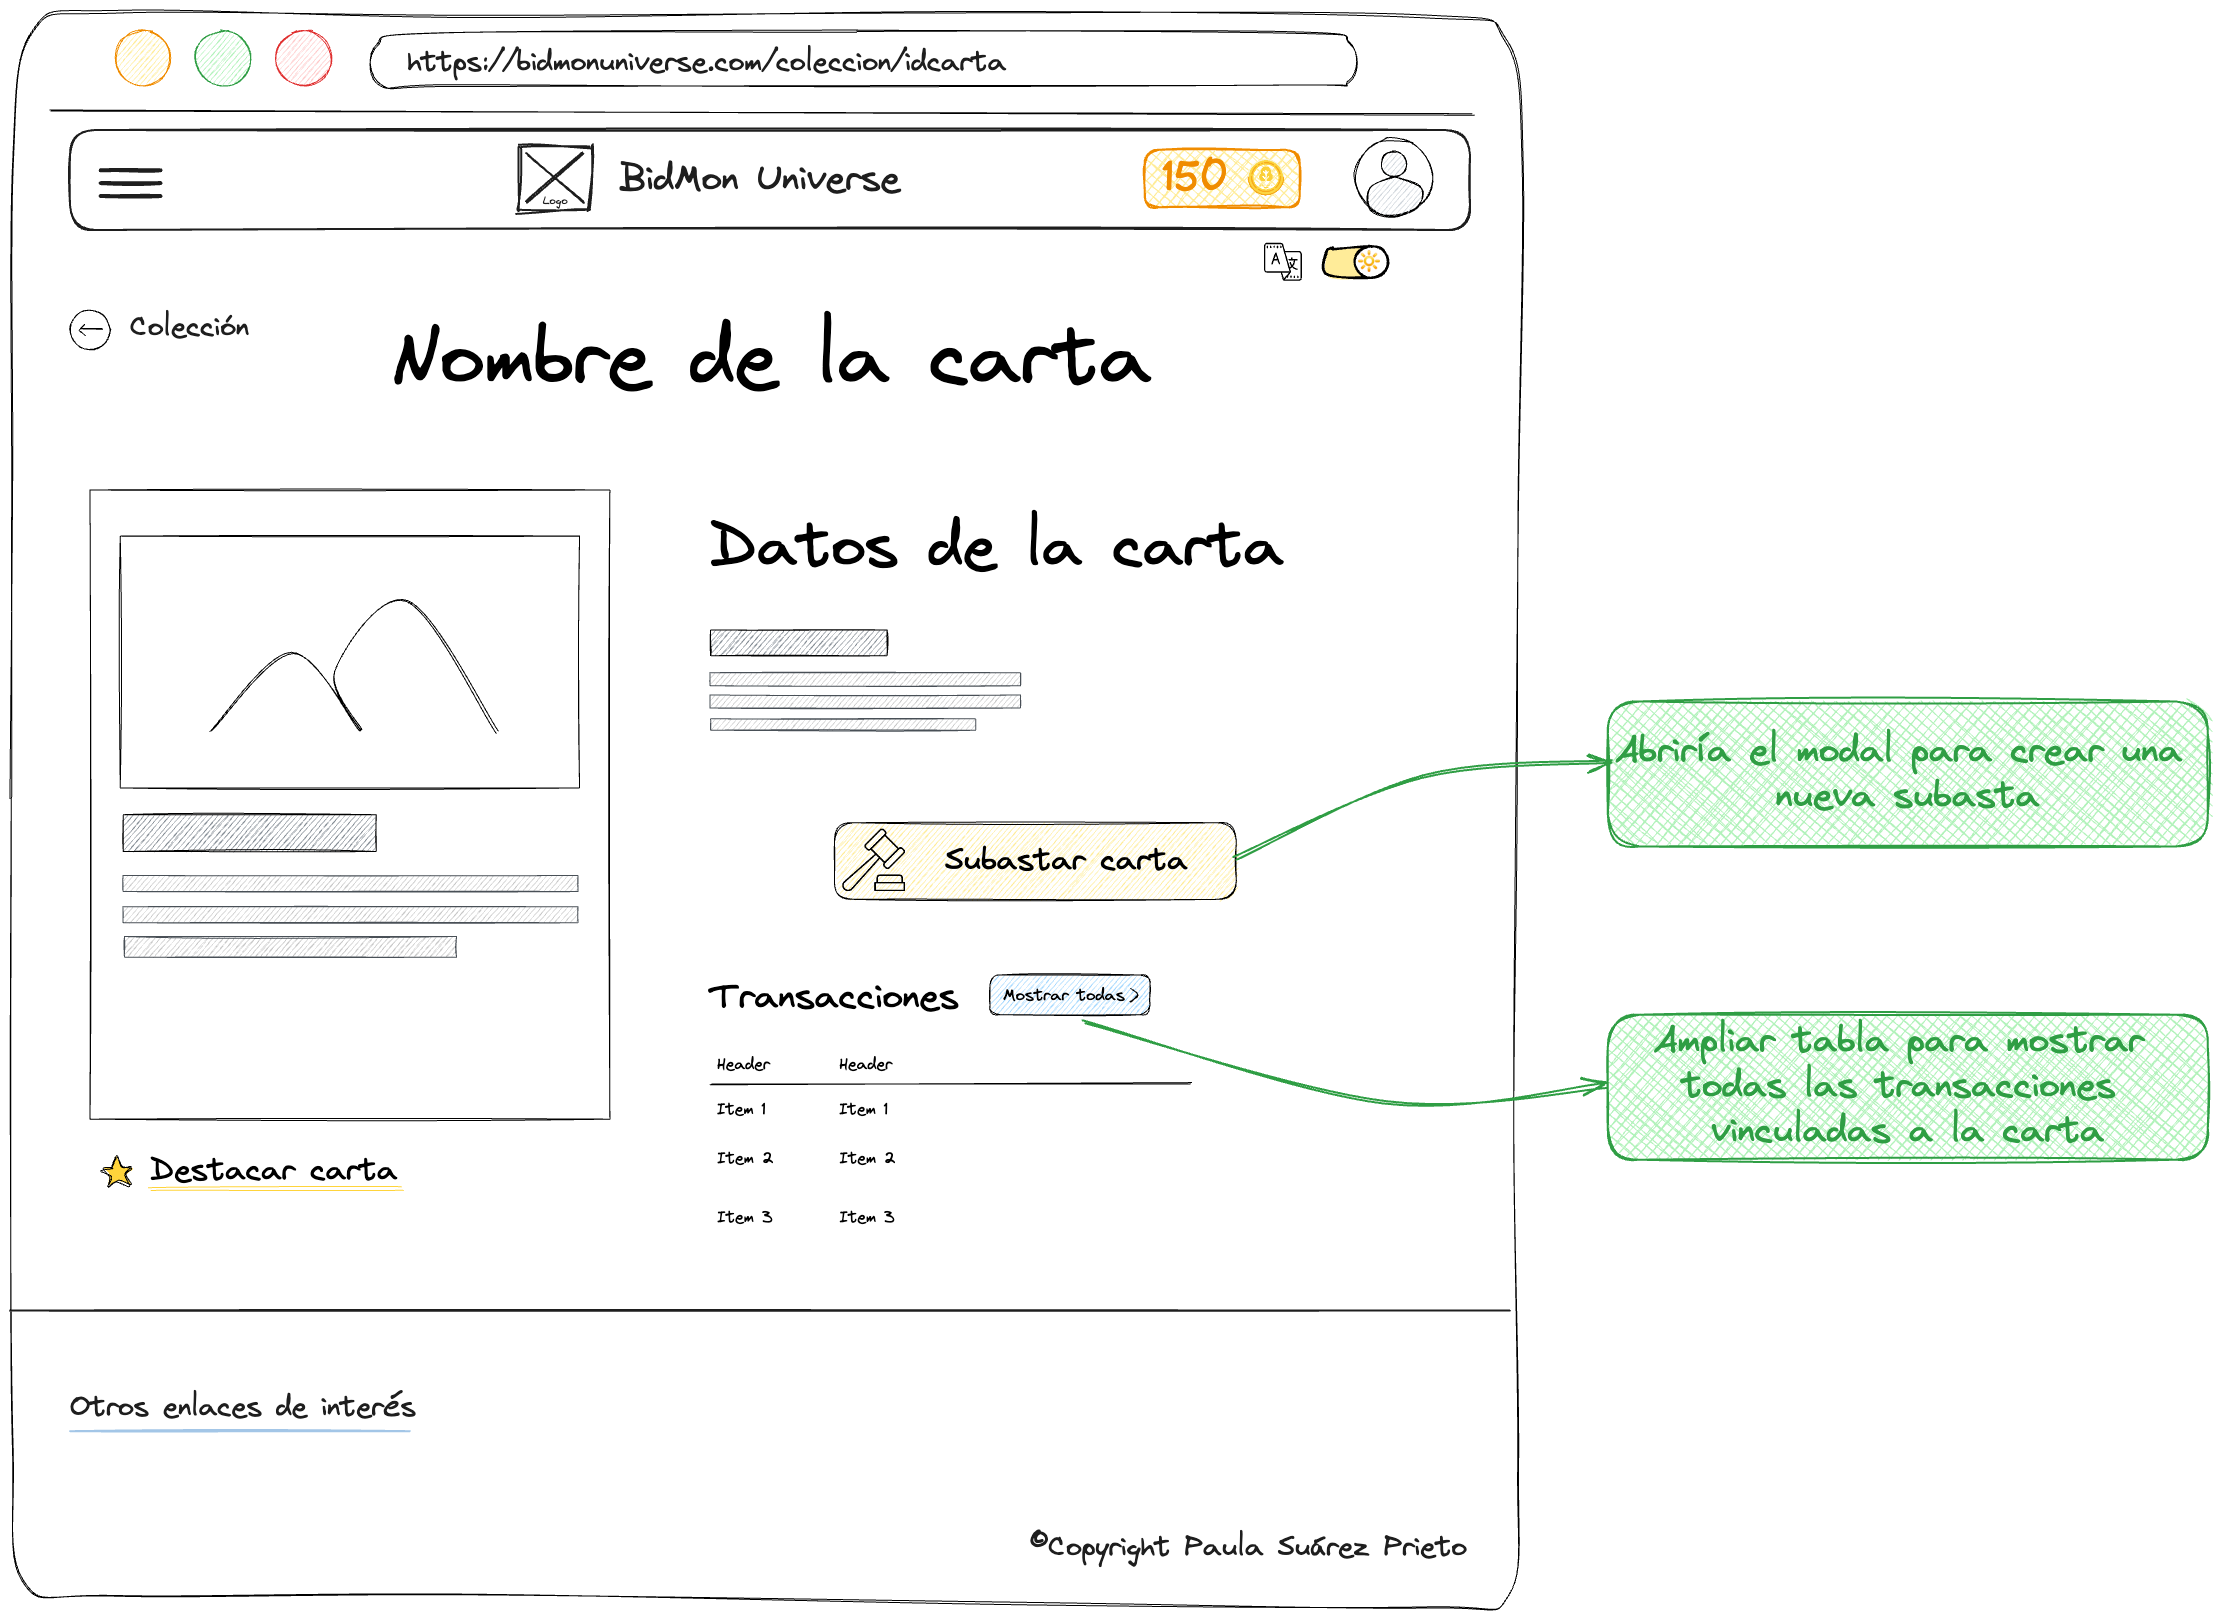
\includegraphics[width=0.9\textwidth]{figures/6-Analisis/6-Interfaz/prototipos/detalle-carta.png}
    \caption{Boceto de la página de detalles de carta}
    \label{fig:p_card_details}
\end{figure}

\subsubsection{Página de Subastas}
La página de subastas muestra una lista de las subastas activas en las que el usuario puede participar.
En esta página hay un menú de navegación que permite al usuario filtrar las subastas por diferentes criterios:
\begin{itemize}
    \item Todas: Todas las subastas activas.
    \item Mis Subastas: Subastas en las que el usuario ha creado.
    \item Pujas: Subastas en las que el usuario ha pujado.
\end{itemize}
La página de subastas muestra las cartas subastadas, al hacer clic en una carta se muestra la información detallada de la subasta.
En la figura \ref{fig:p_auctions} se muestra el boceto de la página de subastas.
\begin{figure}[H]
    \centering
    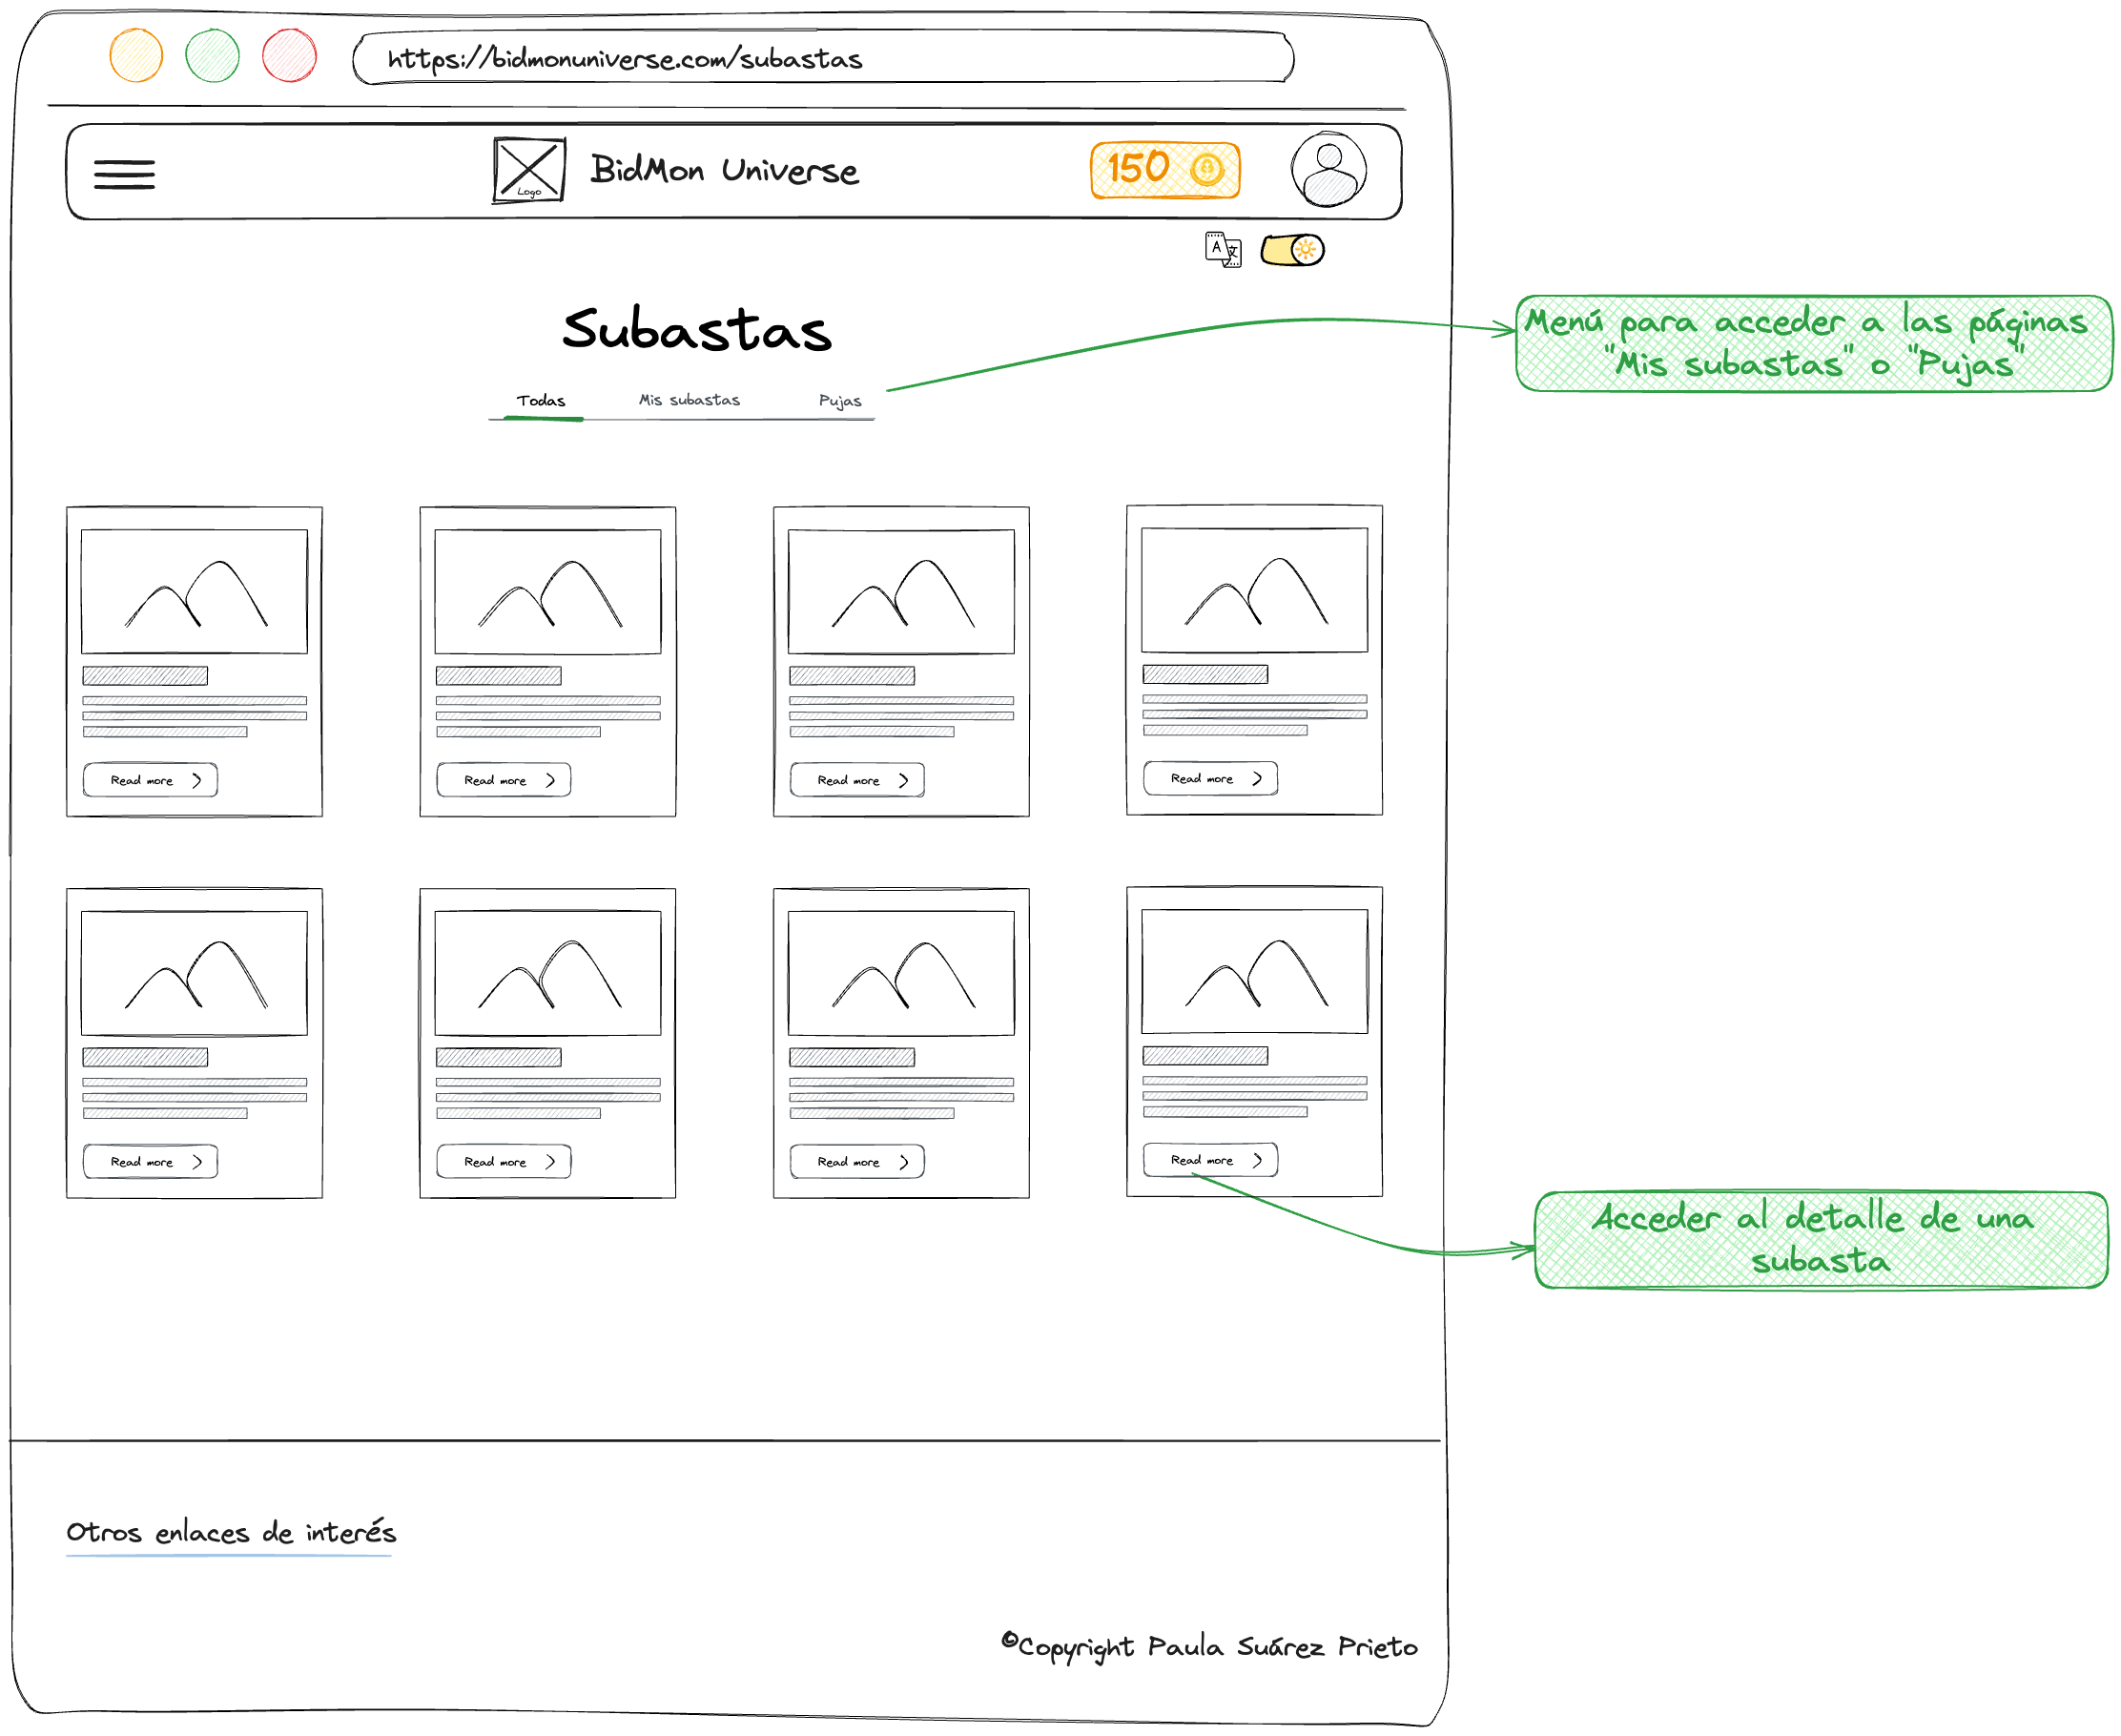
\includegraphics[width=0.9\textwidth]{figures/6-Analisis/6-Interfaz/prototipos/subastas.png}
    \caption{Boceto de la página de subastas}
    \label{fig:p_auctions}
\end{figure}

\subsubsection{Página de Detalles de Subasta}
La página de detalles de subasta muestra información detallada sobre una subasta específica.
Dependiendo de si la subasta es propia o no, el usuario puede realizar diferentes acciones.
En la figura \ref{fig:p_auction_details} se muestra el boceto de la página de detalles de una subasta activa creada por otro usuario.
\begin{figure}[H]
    \centering
    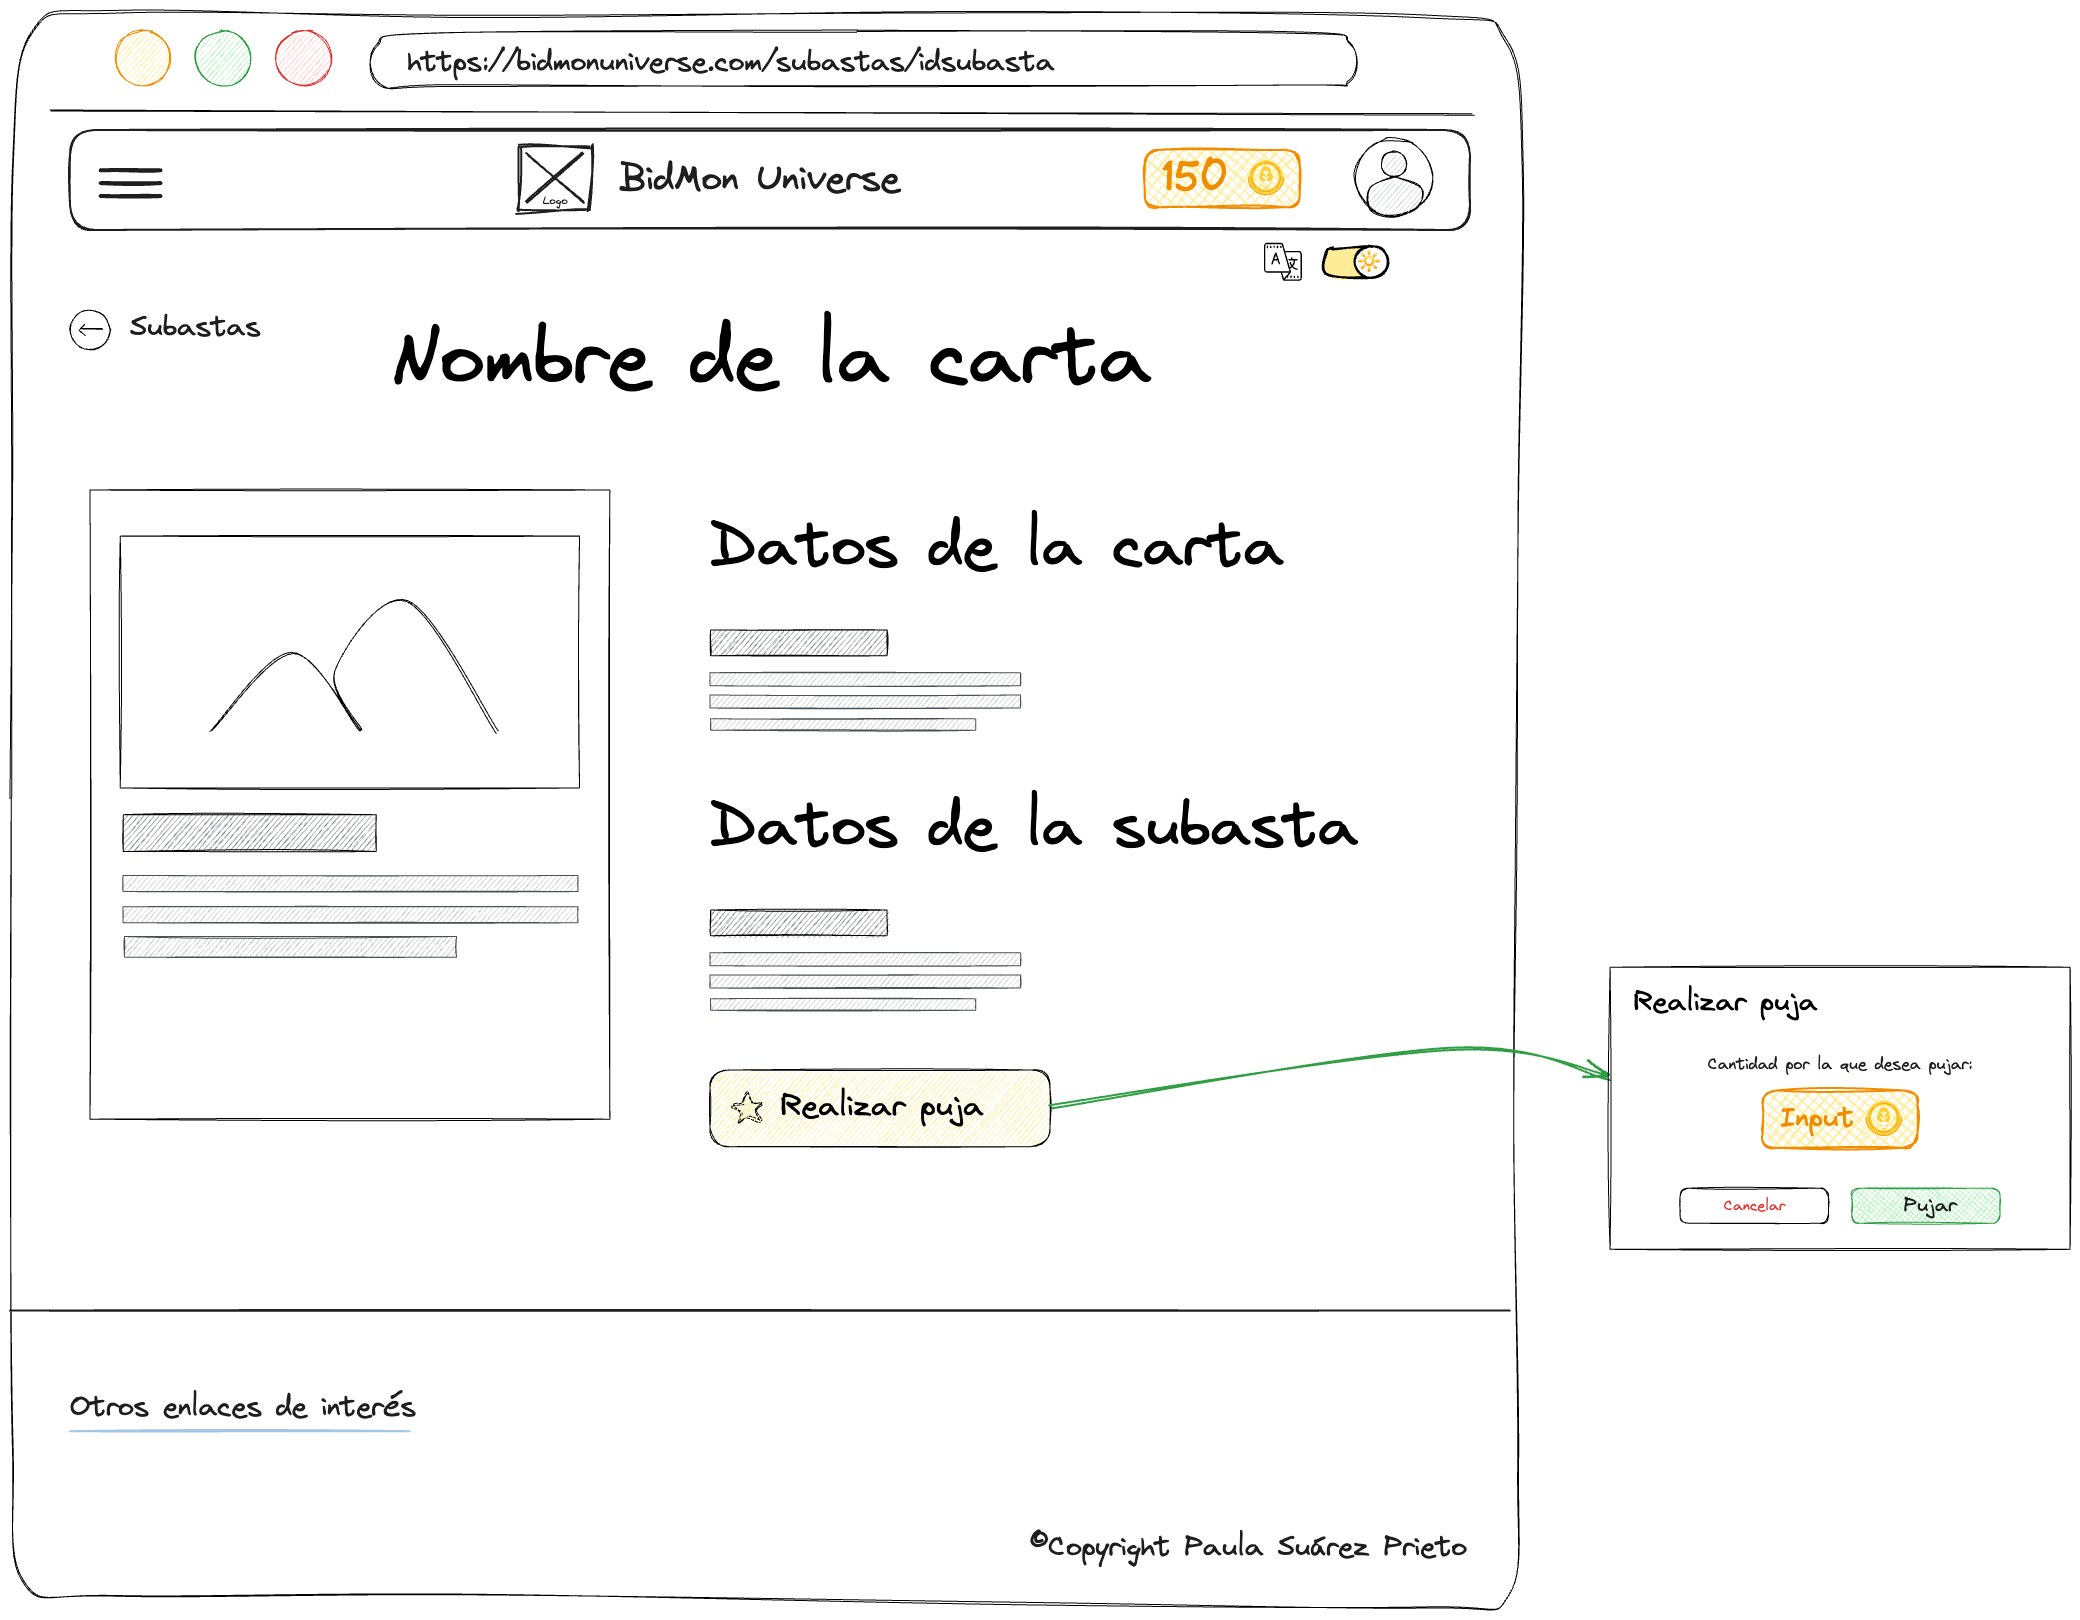
\includegraphics[width=0.9\textwidth]{figures/6-Analisis/6-Interfaz/prototipos/detalle-subasta.png}
    \caption{Boceto de la página de detalles de subasta}
    \label{fig:p_auction_details}
\end{figure}

En el caso de que la subasta sea propia, el usuario puede cancelar la subasta como se muestra en la figura \ref{fig:p_auction_details_own}.
\begin{figure}[H]
    \centering
    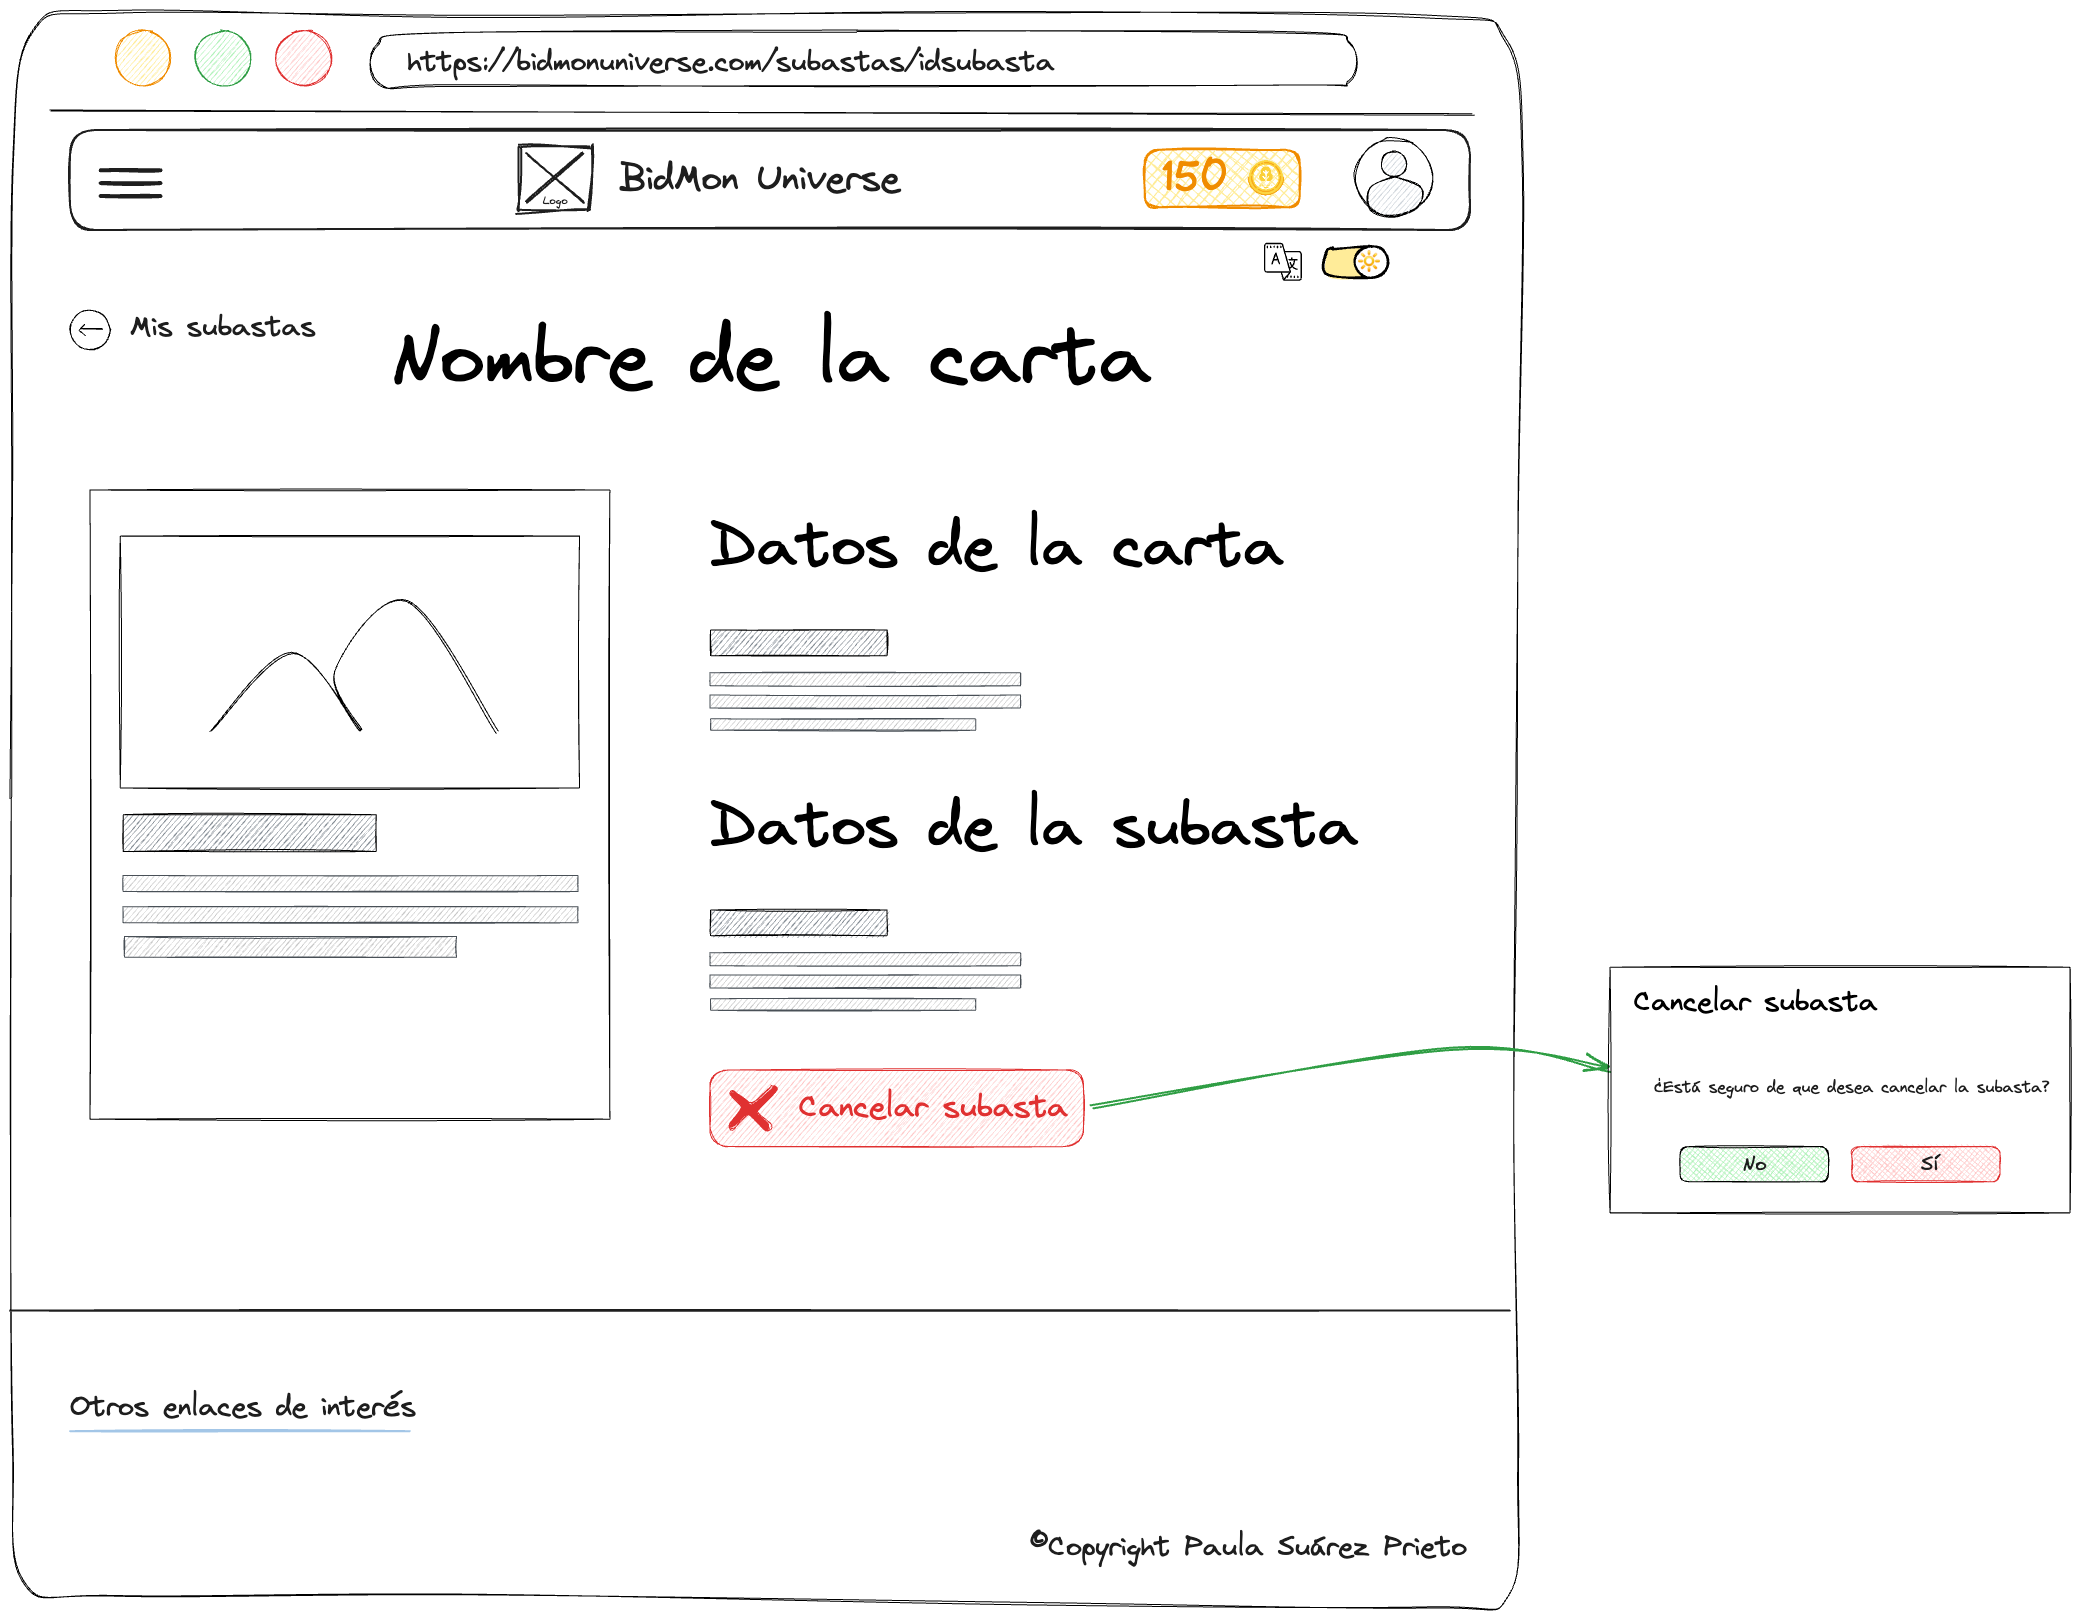
\includegraphics[width=0.9\textwidth]{figures/6-Analisis/6-Interfaz/prototipos/detalle-subasta-propia.png}
    \caption{Boceto de la página de detalles de subasta propia}
    \label{fig:p_auction_details_own}
\end{figure}

En el caso de que sea una subasta en la que el usuario ha pujado, el usuario puede retirar la puja como se muestra en la figura \ref{fig:p_auction_details_bid}.
\begin{figure}[H]
    \centering
    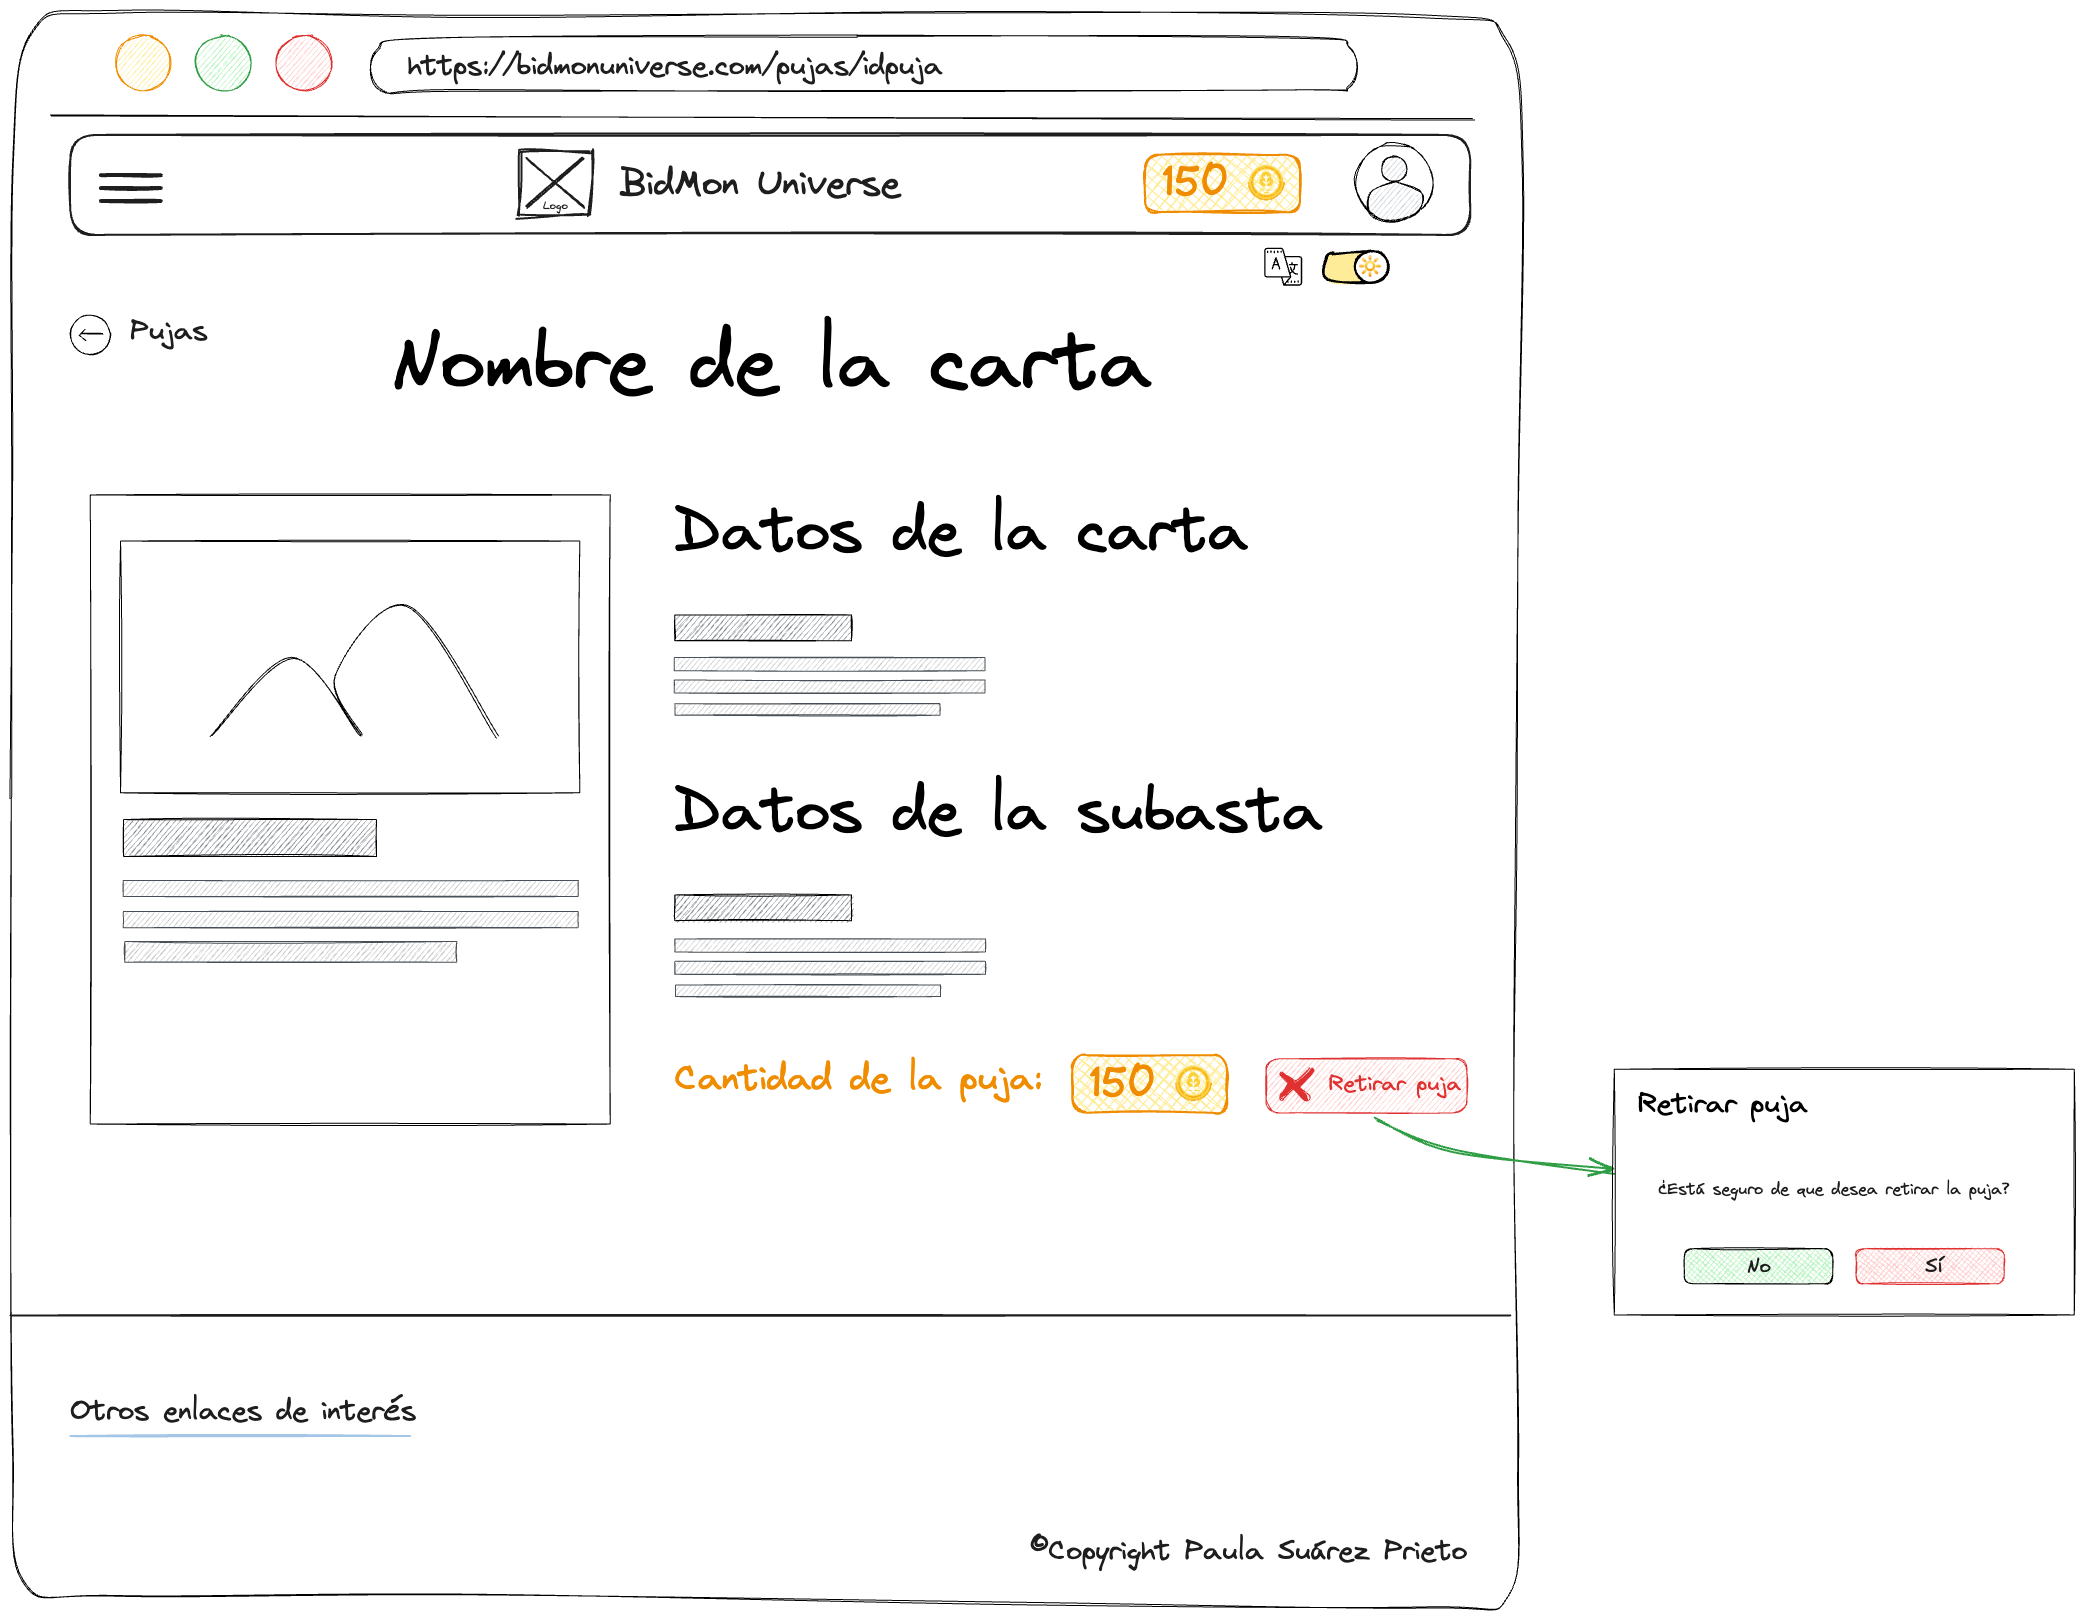
\includegraphics[width=0.9\textwidth]{figures/6-Analisis/6-Interfaz/prototipos/detalle-puja.png}
    \caption{Boceto de la página de detalles de subasta en la que el usuario ha pujado}
    \label{fig:p_auction_details_bid}
\end{figure}

\subsubsection{Página de Histórico de Transacciones}
La página de histórico de transacciones muestra una lista de las transacciones realizadas.
Si el usuario que ha iniciado sesión es un administrador, se mostrarán todas las transacciones realizadas en el sistema.
Si el usuario que ha iniciado sesión es un usuario normal, se mostrarán solo las transacciones realizadas por él.
En la figura \ref{fig:p_transactions} se muestra el boceto de la página de histórico de transacciones.
\begin{figure}[H]
    \centering
    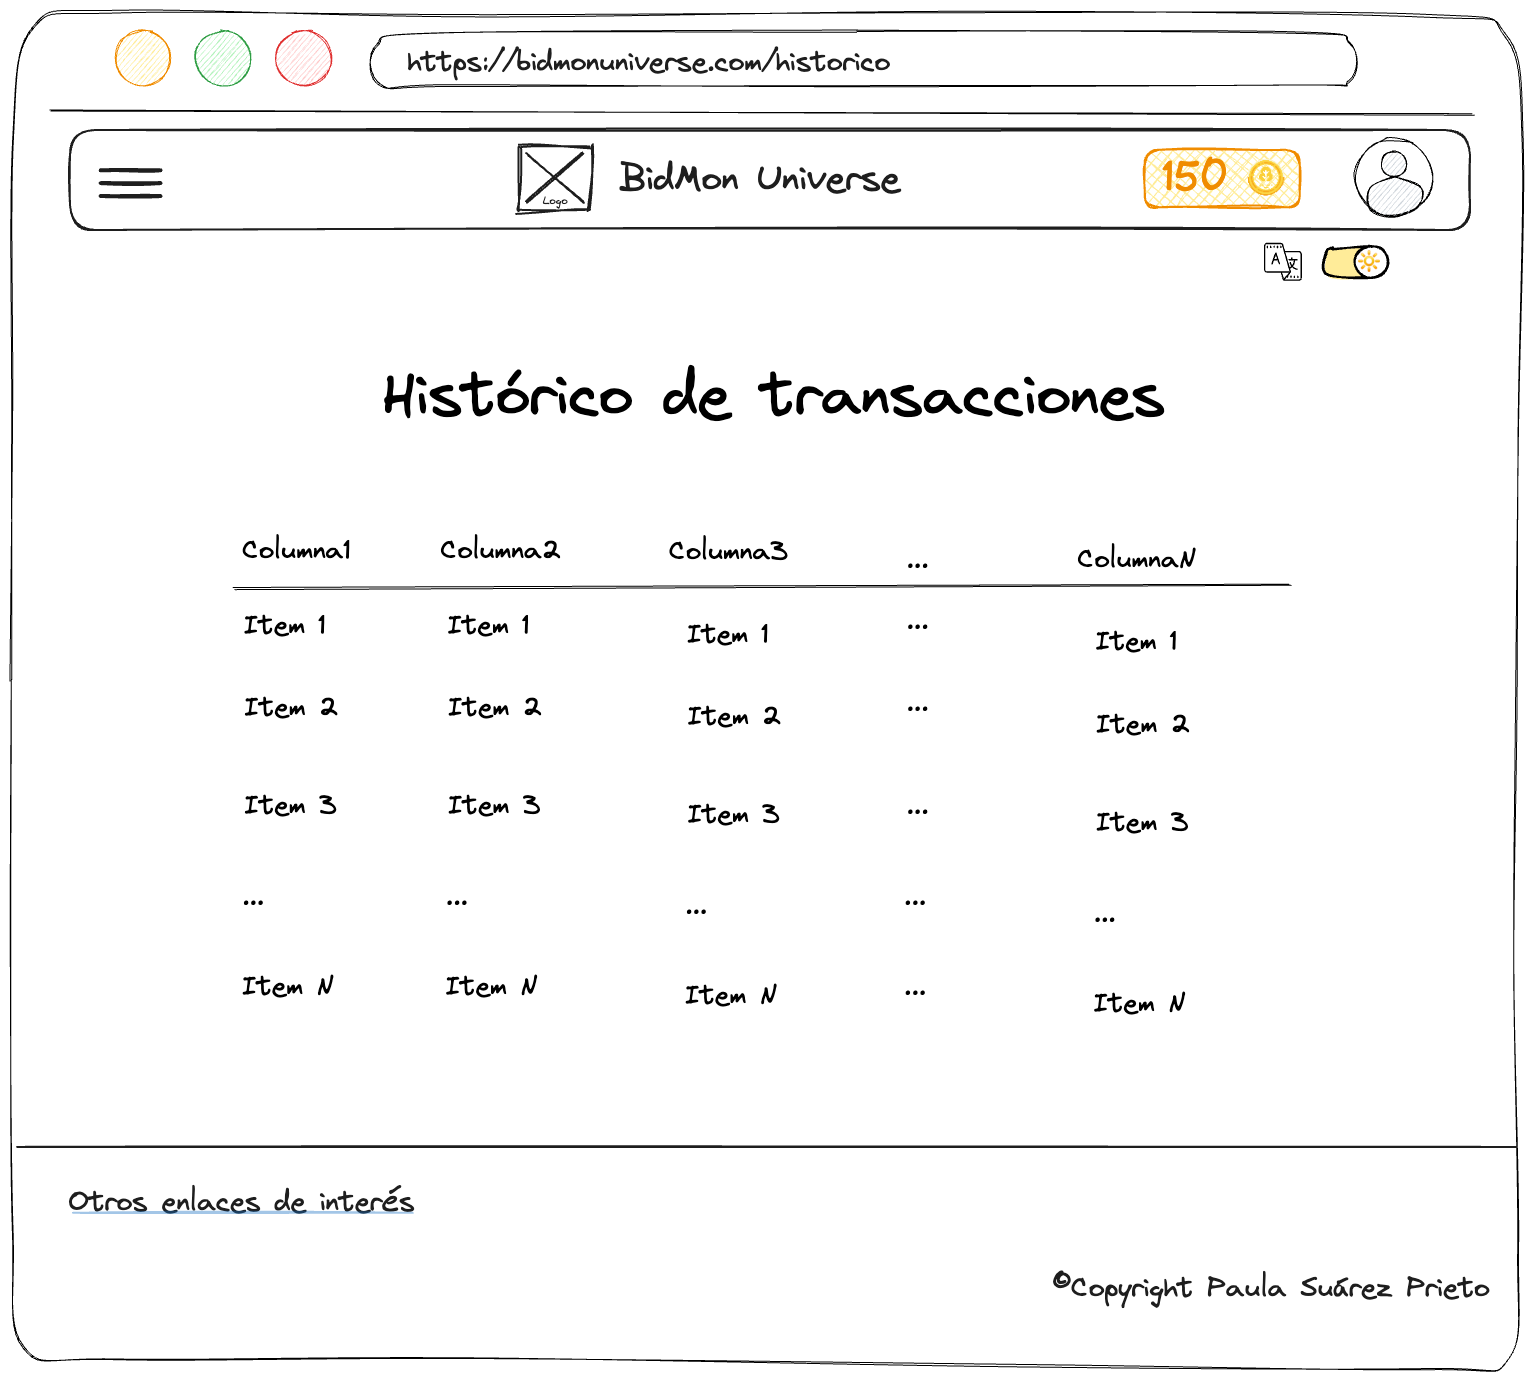
\includegraphics[width=0.9\textwidth]{figures/6-Analisis/6-Interfaz/prototipos/historico-transacciones.png}
    \caption{Boceto de la página de histórico de transacciones}
    \label{fig:p_transactions}
\end{figure}

\subsection{Definición del aspecto de la interfaz}
Se ha creado la interfaz en base a los bocetos de la sección anterior.
La interfaz se ha desarrollado en React.

\subsubsection{Descripción de los recursos empleados en la interfaz}
La primera tarea que se ha realizado ha sido la de definir los colores y tipografías que se van a utilizar en la interfaz.
Se ha elegido la tipografía \textit{Pokemon Hollow} para el título de la aplicación y para la bienvenida al usuario.

El logo de la aplicación se ha generado mediante inteligencia artificial, utilizando la herramienta \coloredUnderline{\href{https://openai.com/chatgpt/}{ChatGPT}}.
, al igual que el \textit{favicon} de la aplicación.

Los avatares que se pueden seleccionar como imagen de perfil se han obtenido de la página web \coloredUnderline{\href{https://www.behance.net/gallery/10774061/Pokmon-Avatars}{Behance, Pokémon Avatars de Mikeel Araña}}.

Las imágenes de las medallas de los gimnasios se han obtenido de la página web \coloredUnderline{\href{https://www.wikidex.net/wiki/Líder_de_gimnasio}{Wikidex}}.

Los iconos de los tipos de Pokémon se han obtenido del repositorio \coloredUnderline{\href{https://github.com/duiker101/pokemon-type-svg-icons}{pokemon-type-svg-icons, de duiker101}}.

Las imágenes de los Pokémon se han obtenido de la página web \coloredUnderline{\href{https://pokeapi.co/}{PokéAPI}}.

Para implementar la interfaz se ha utilizado principalmente la biblioteca \coloredUnderline{\href{https://material-ui.com/}{Material-UI}}. 


\subsubsection{Interfaz de la aplicación}
A continuación se muestran las pantallas de las páginas principales de la aplicación.
Pueden diferir ligeramente de los bocetos iniciales, ya que se han realizado ajustes para mejorar la usabilidad y la estética de la aplicación.

\begin{figure}[H]
    \centering
    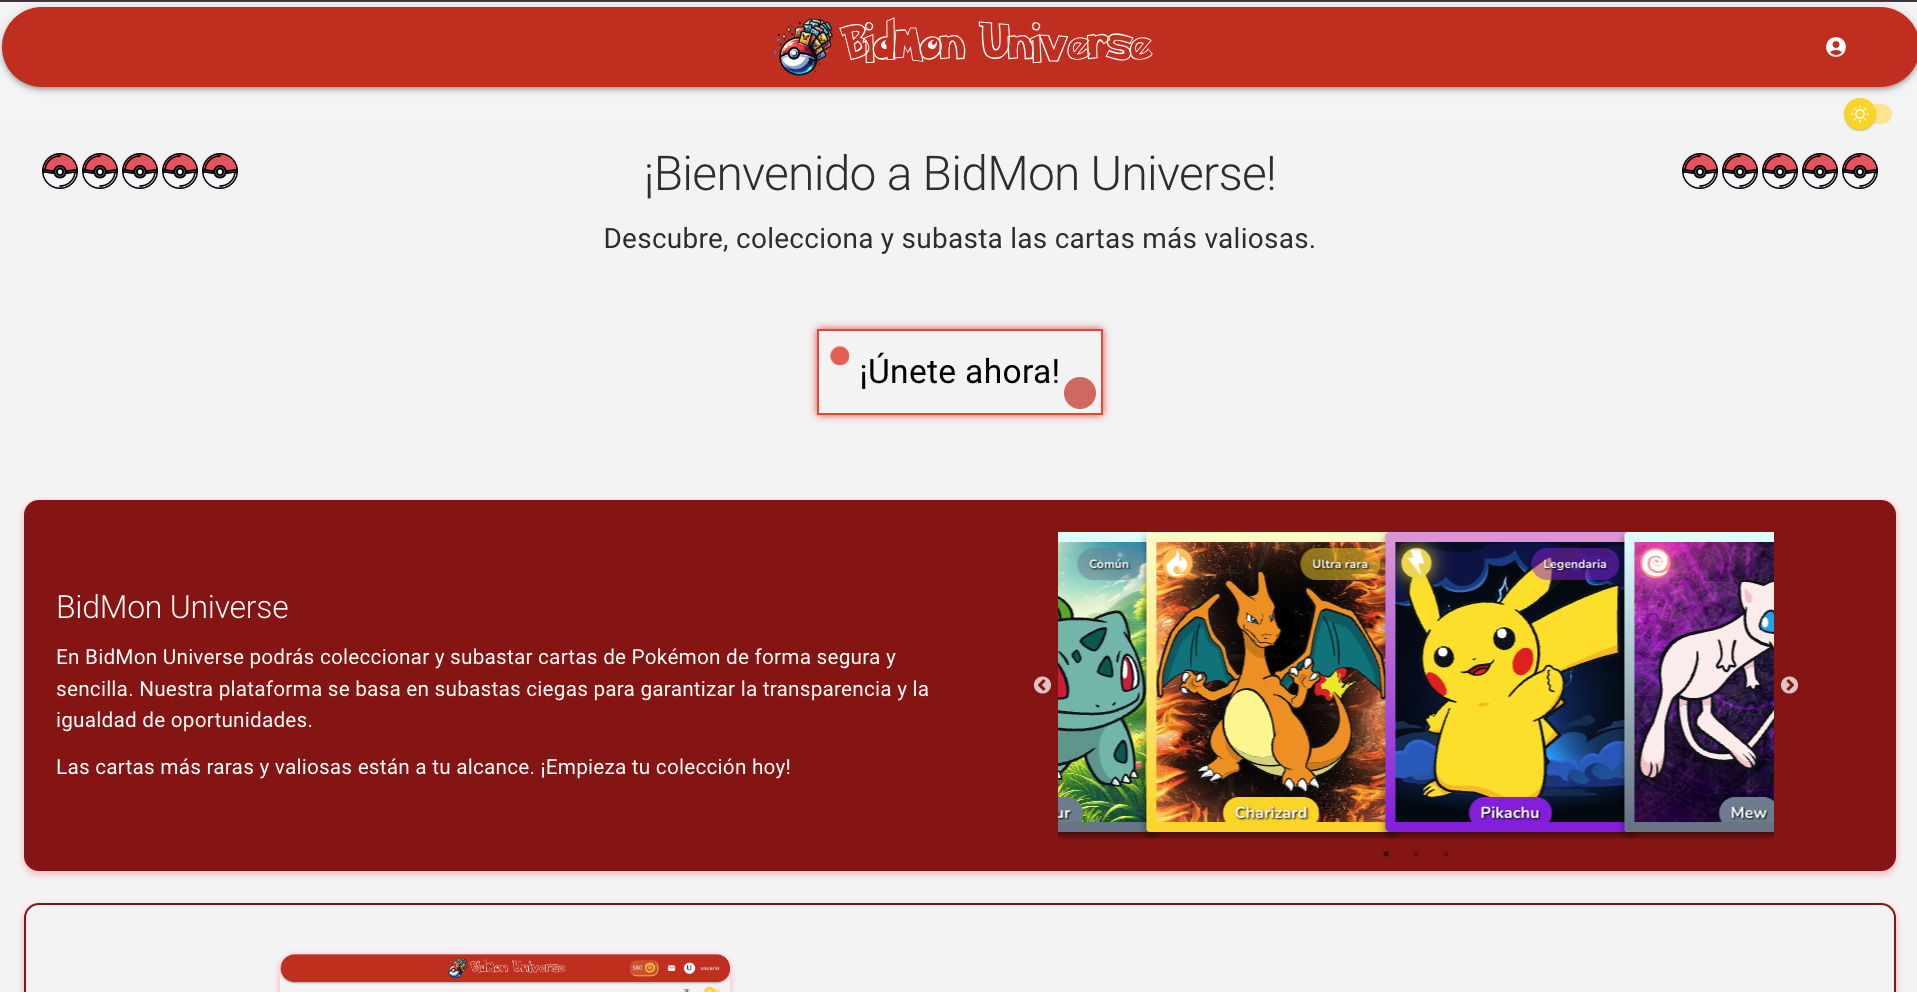
\includegraphics[width=0.8\textwidth]{figures/6-Analisis/6-Interfaz/interfaz/home.png}
    \caption{Página Home, página de inicio de la aplicación.}
    \label{fig:interfaz-home}
\end{figure}

\begin{figure}[H]
    \centering
    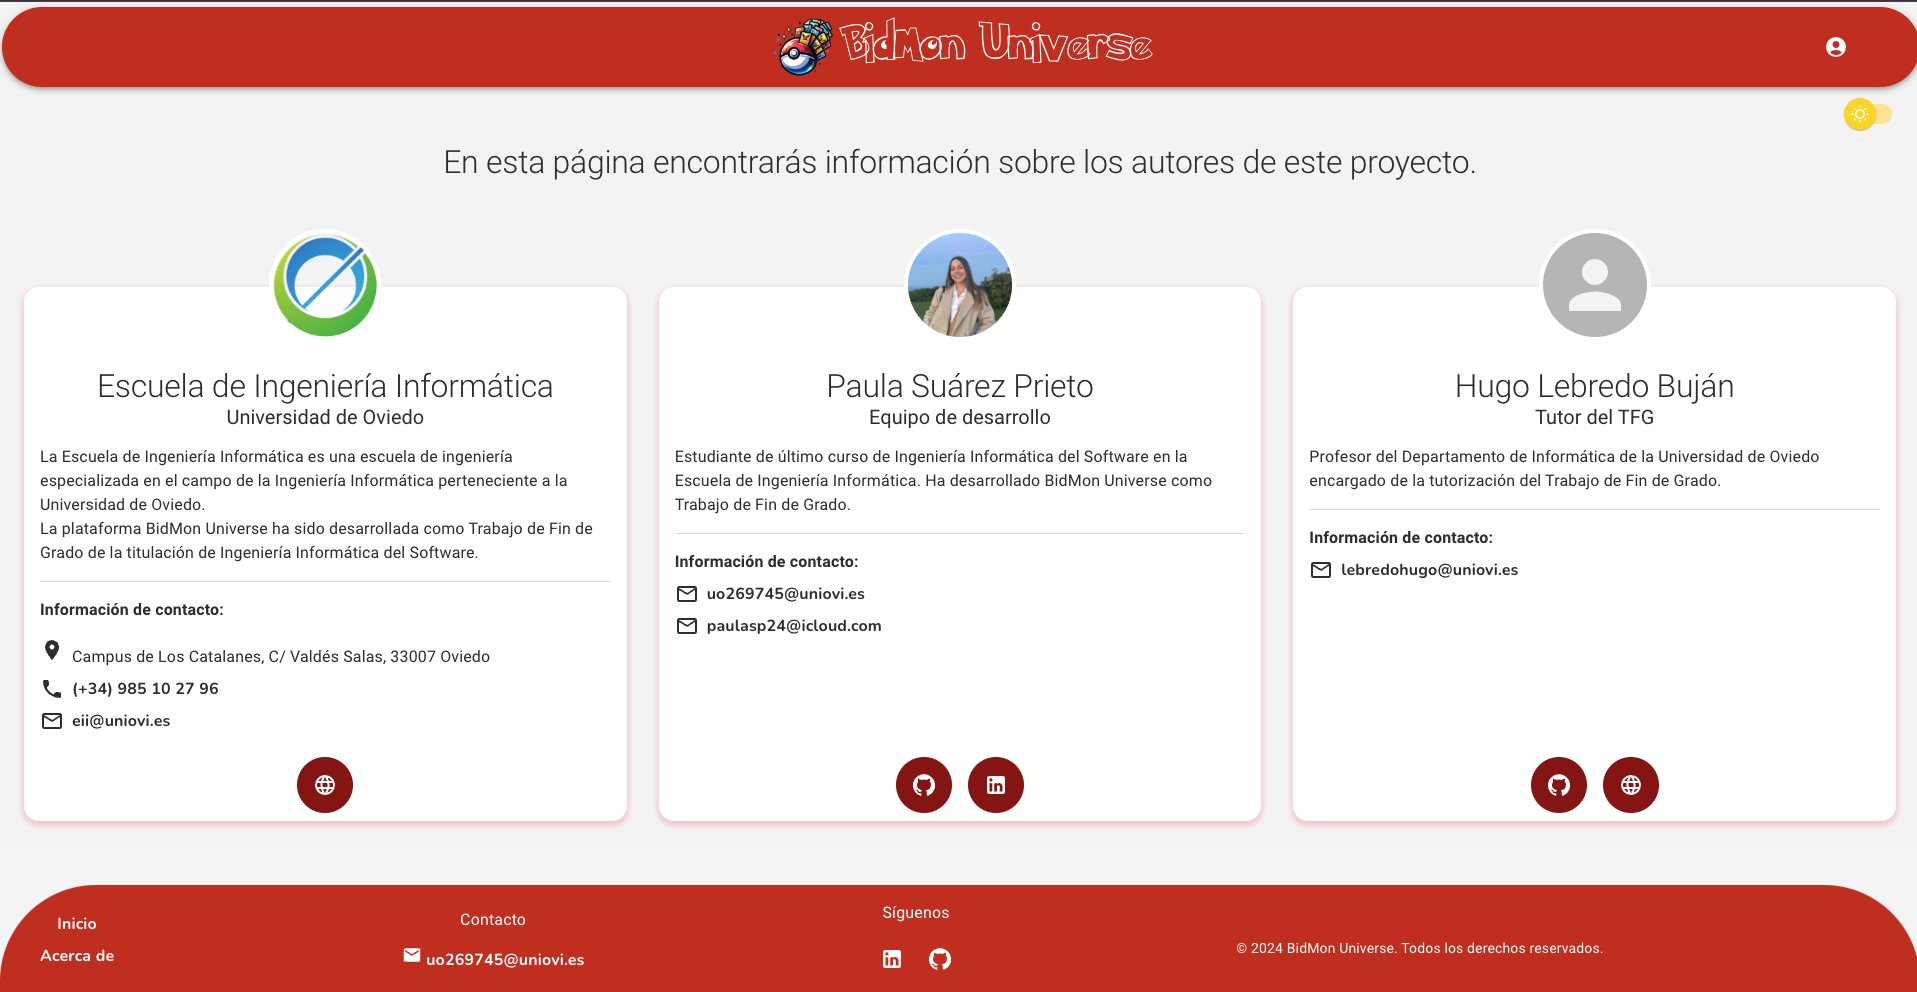
\includegraphics[width=0.8\textwidth]{figures/6-Analisis/6-Interfaz/interfaz/about.png}
    \caption{Página de información sobre la aplicación.}
    \label{fig:interfaz-about}
\end{figure}

\begin{figure}[H]
    \centering
    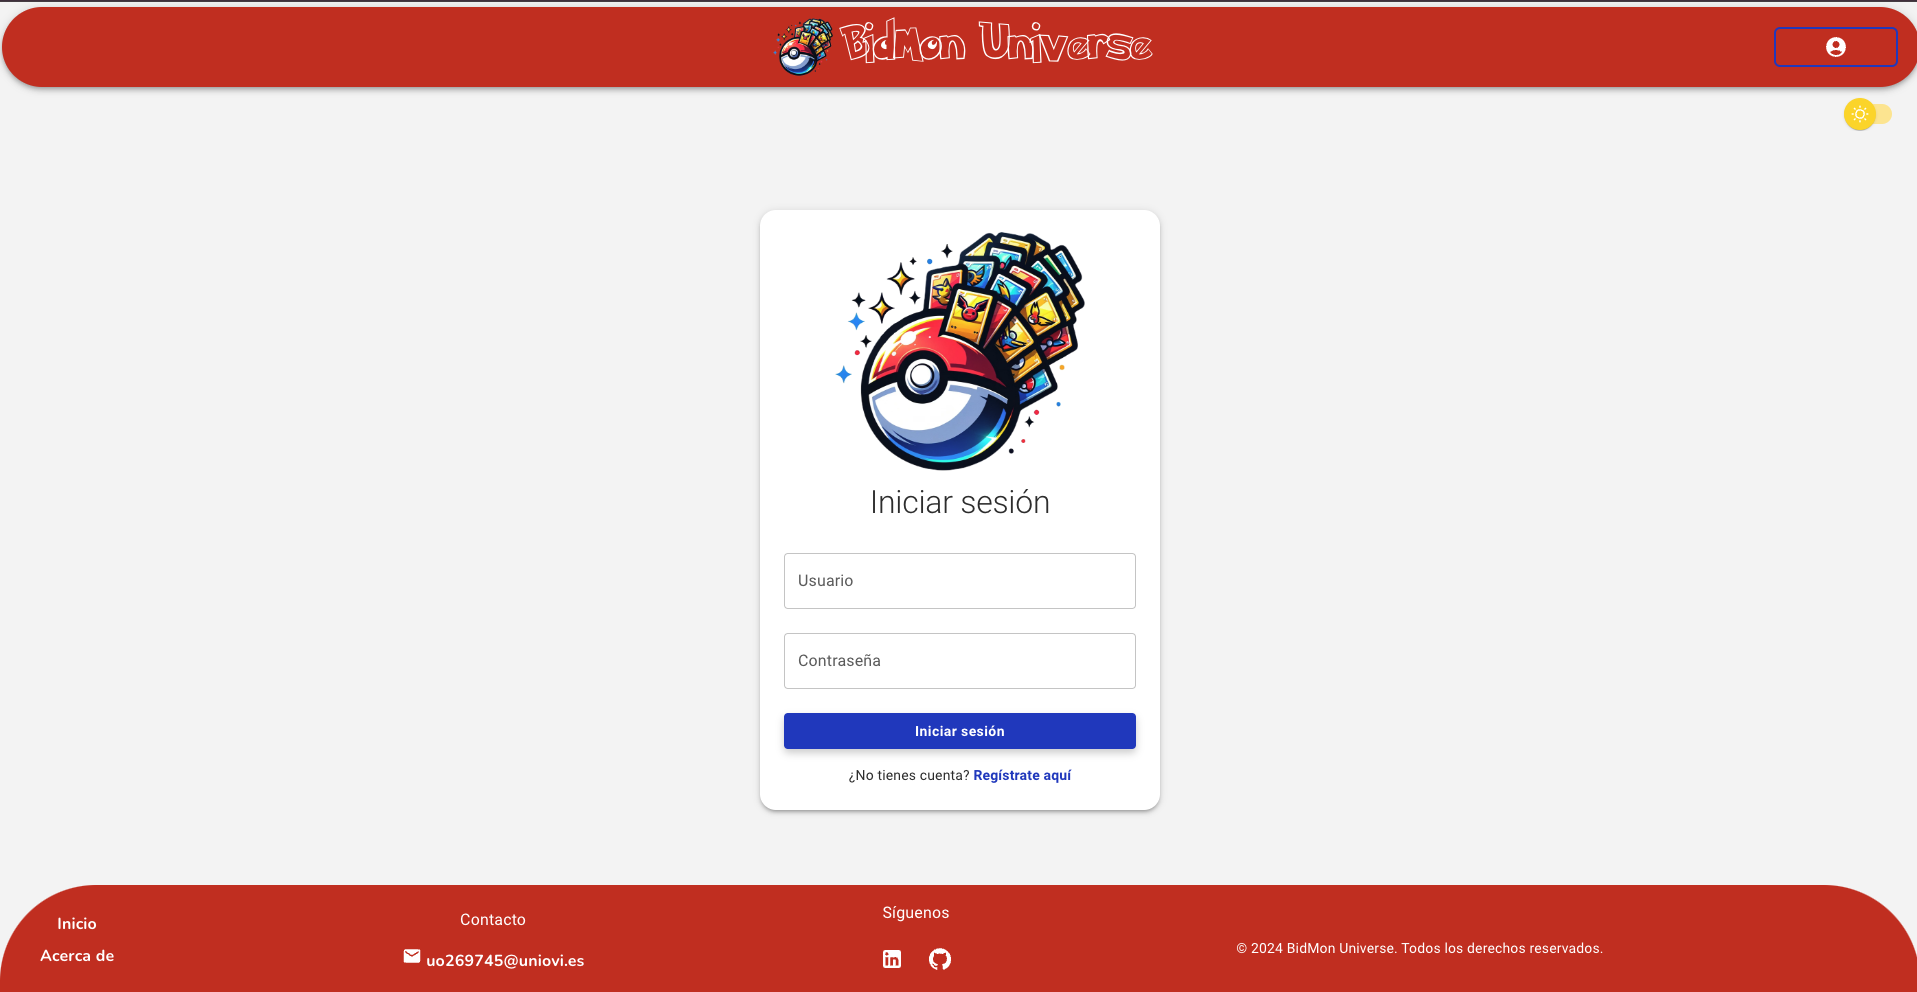
\includegraphics[width=0.8\textwidth]{figures/6-Analisis/6-Interfaz/interfaz/login.png}
    \caption{Página de inicio de sesión.}
    \label{fig:interfaz-login}
\end{figure}

\begin{figure}[H]
    \centering
    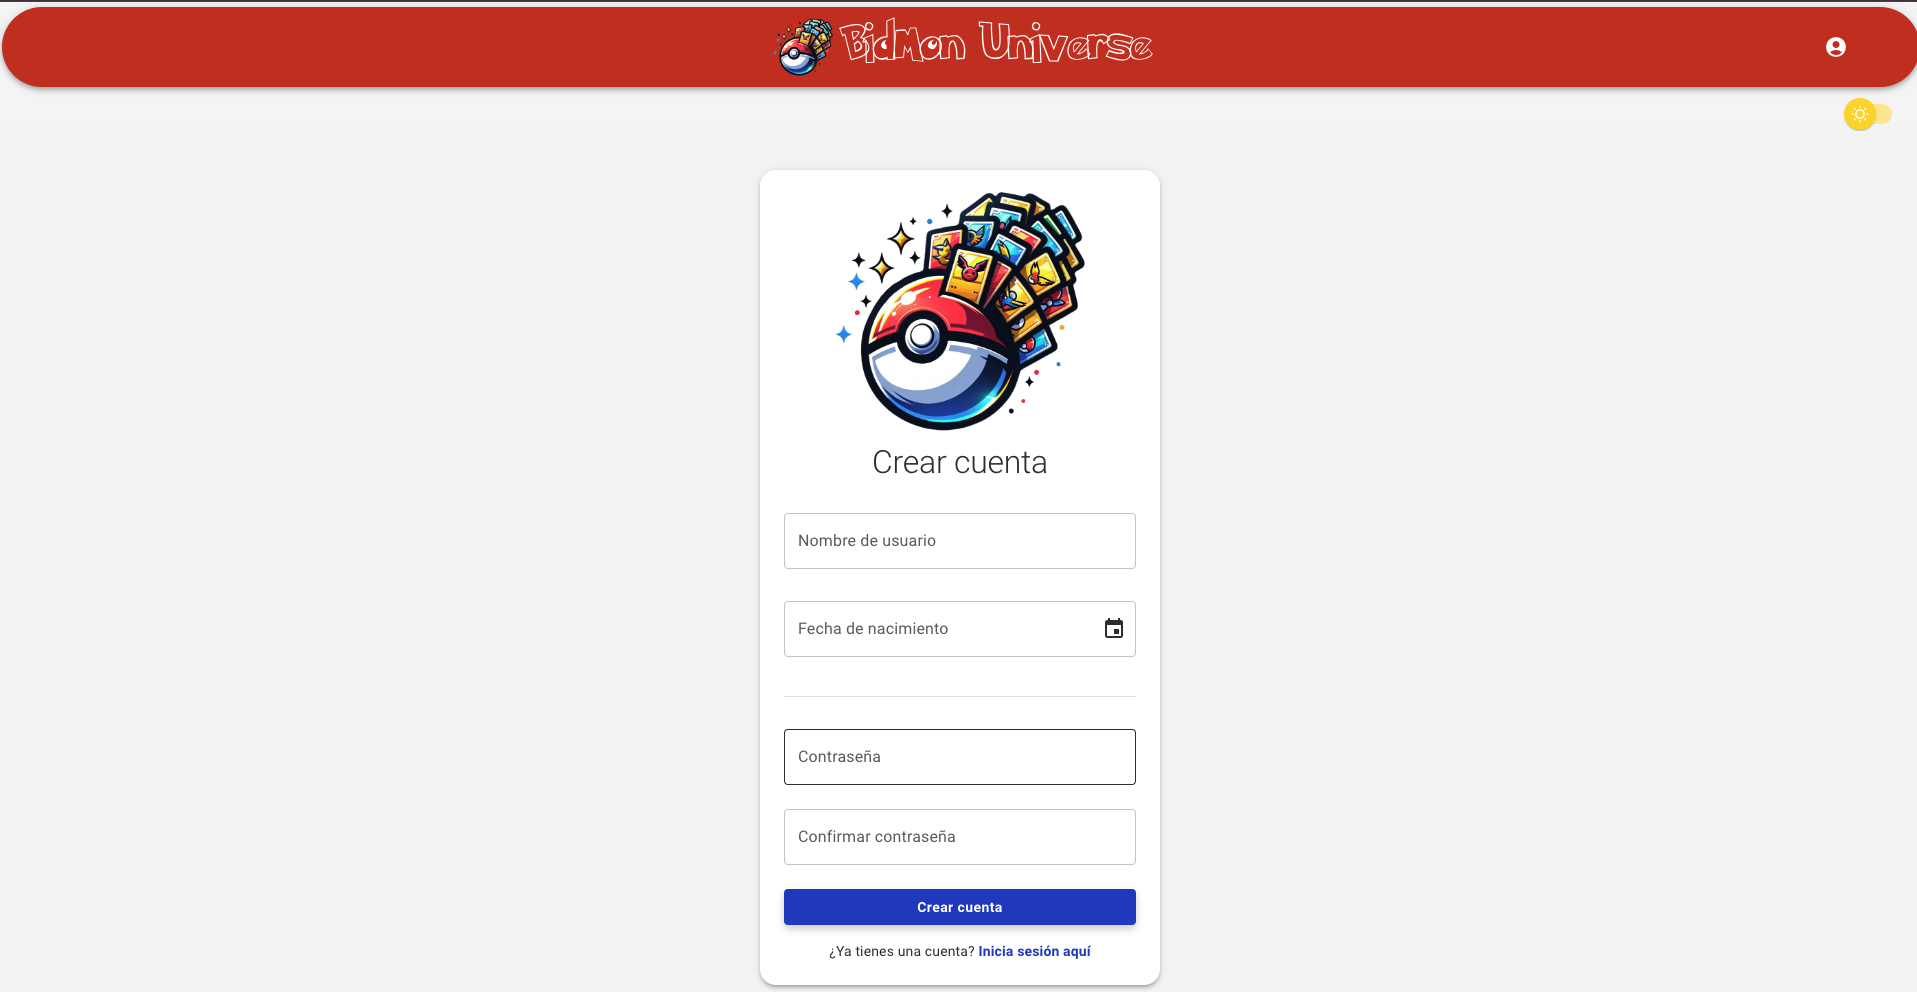
\includegraphics[width=0.8\textwidth]{figures/6-Analisis/6-Interfaz/interfaz/signup.png}
    \caption{Página de registro de usuario.}
    \label{fig:interfaz-registro}
\end{figure}

\begin{figure}[H]
    \centering
    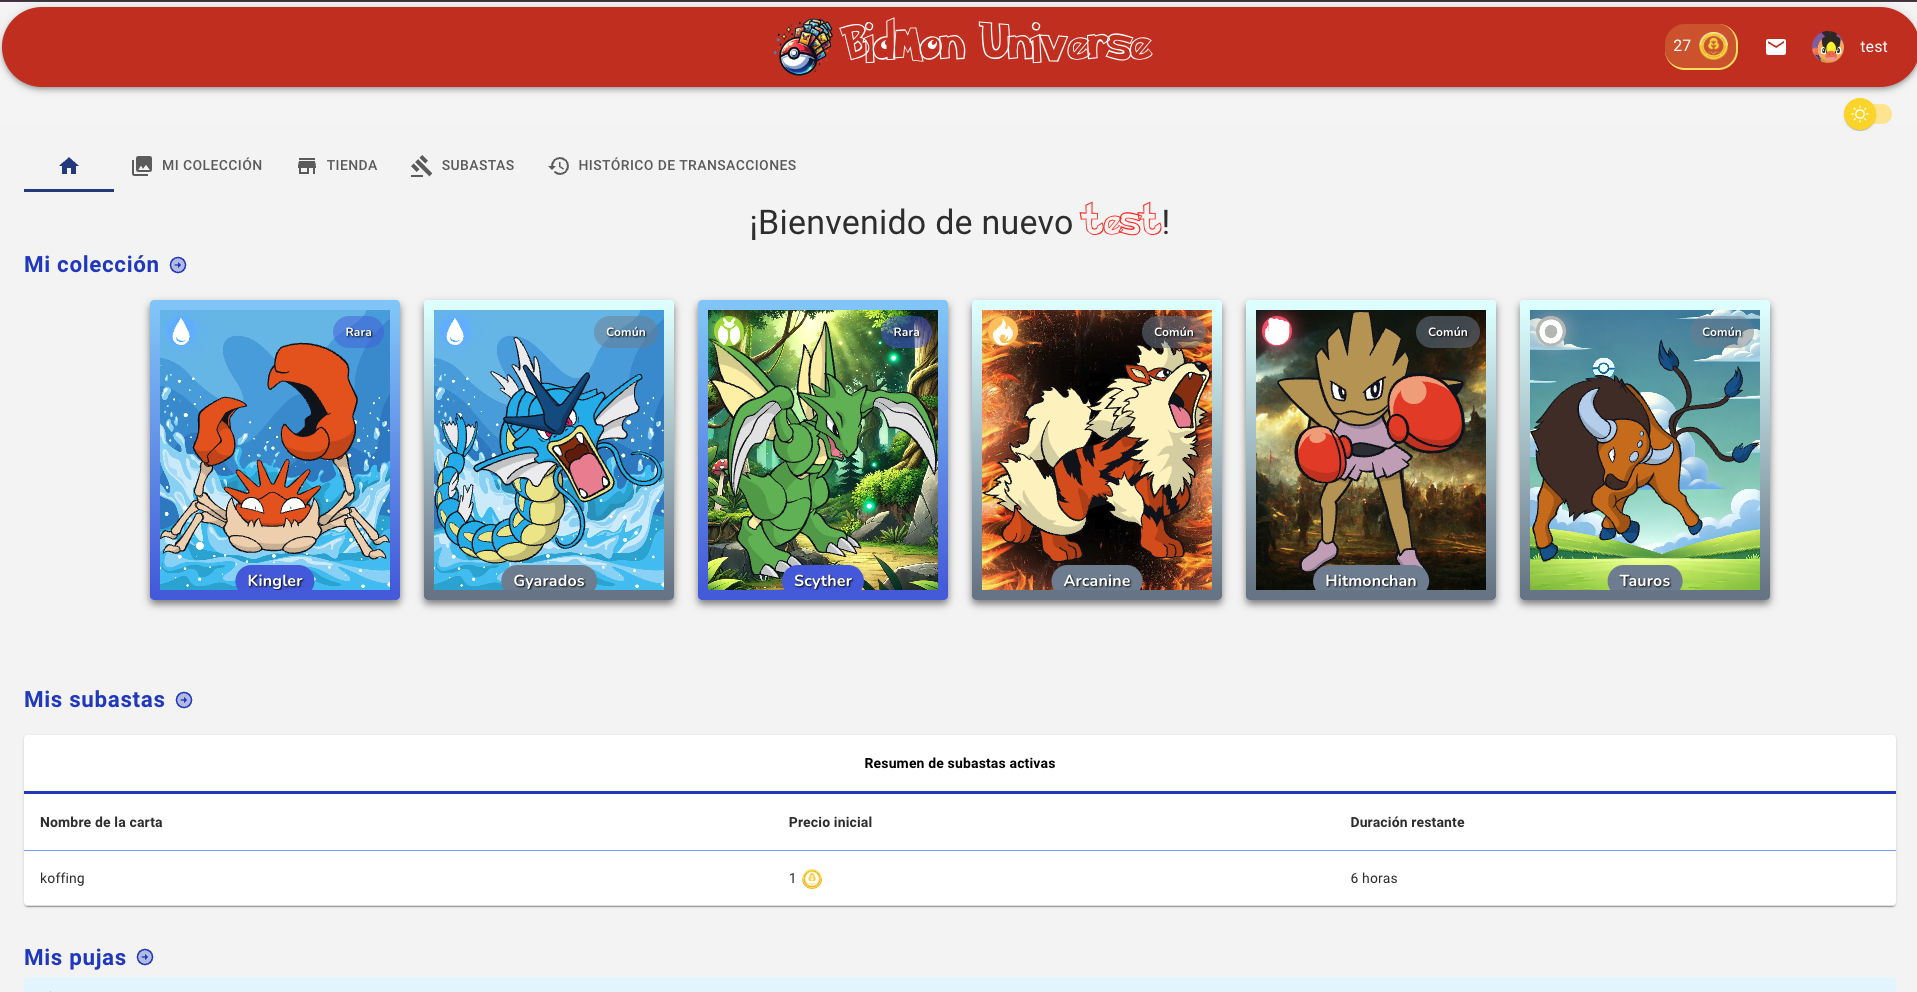
\includegraphics[width=0.8\textwidth]{figures/6-Analisis/6-Interfaz/interfaz/logued.png}
    \caption{Página principal de la aplicación, una vez que el usuario ha iniciado sesión.}
    \label{fig:interfaz-logued}
\end{figure}


\begin{figure}[H]
    \centering
    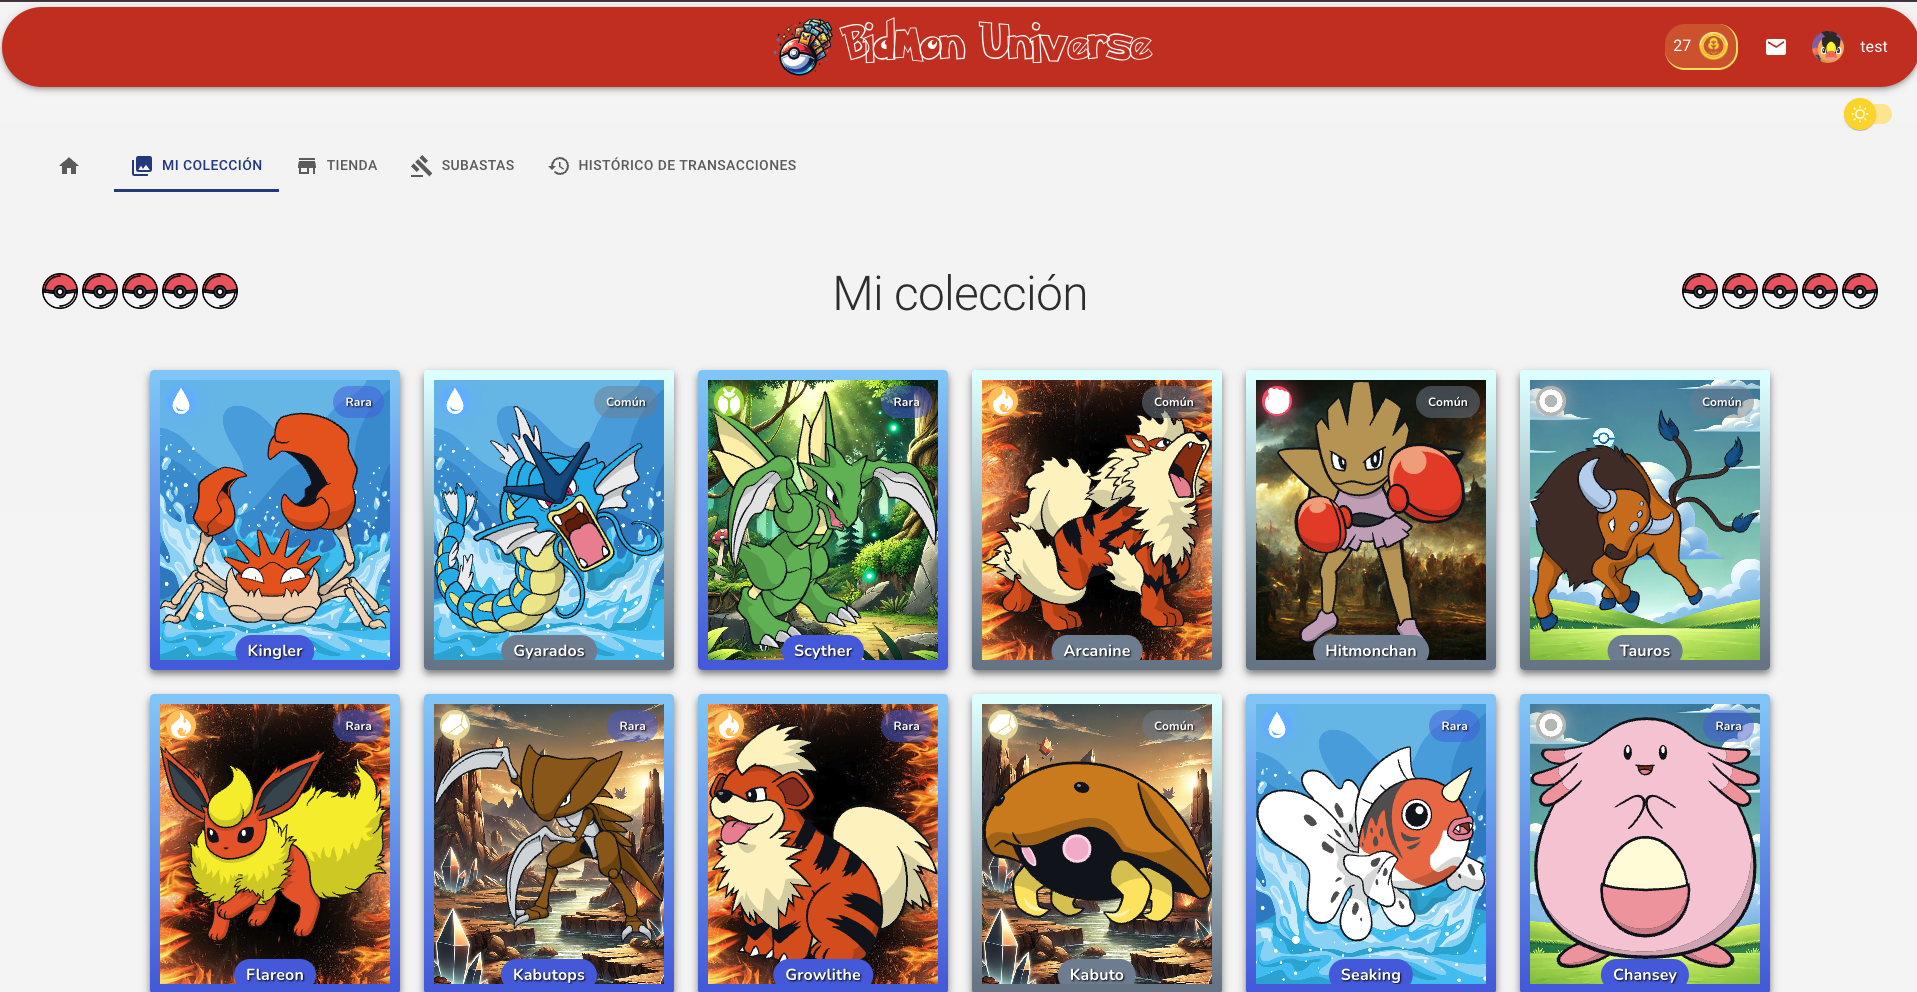
\includegraphics[width=0.8\textwidth]{figures/6-Analisis/6-Interfaz/interfaz/coleccion.png}
    \caption{Página de la colección de cartas del usuario.}
    \label{fig:interfaz-coleccion}
\end{figure}


\begin{figure}[H]
    \centering
    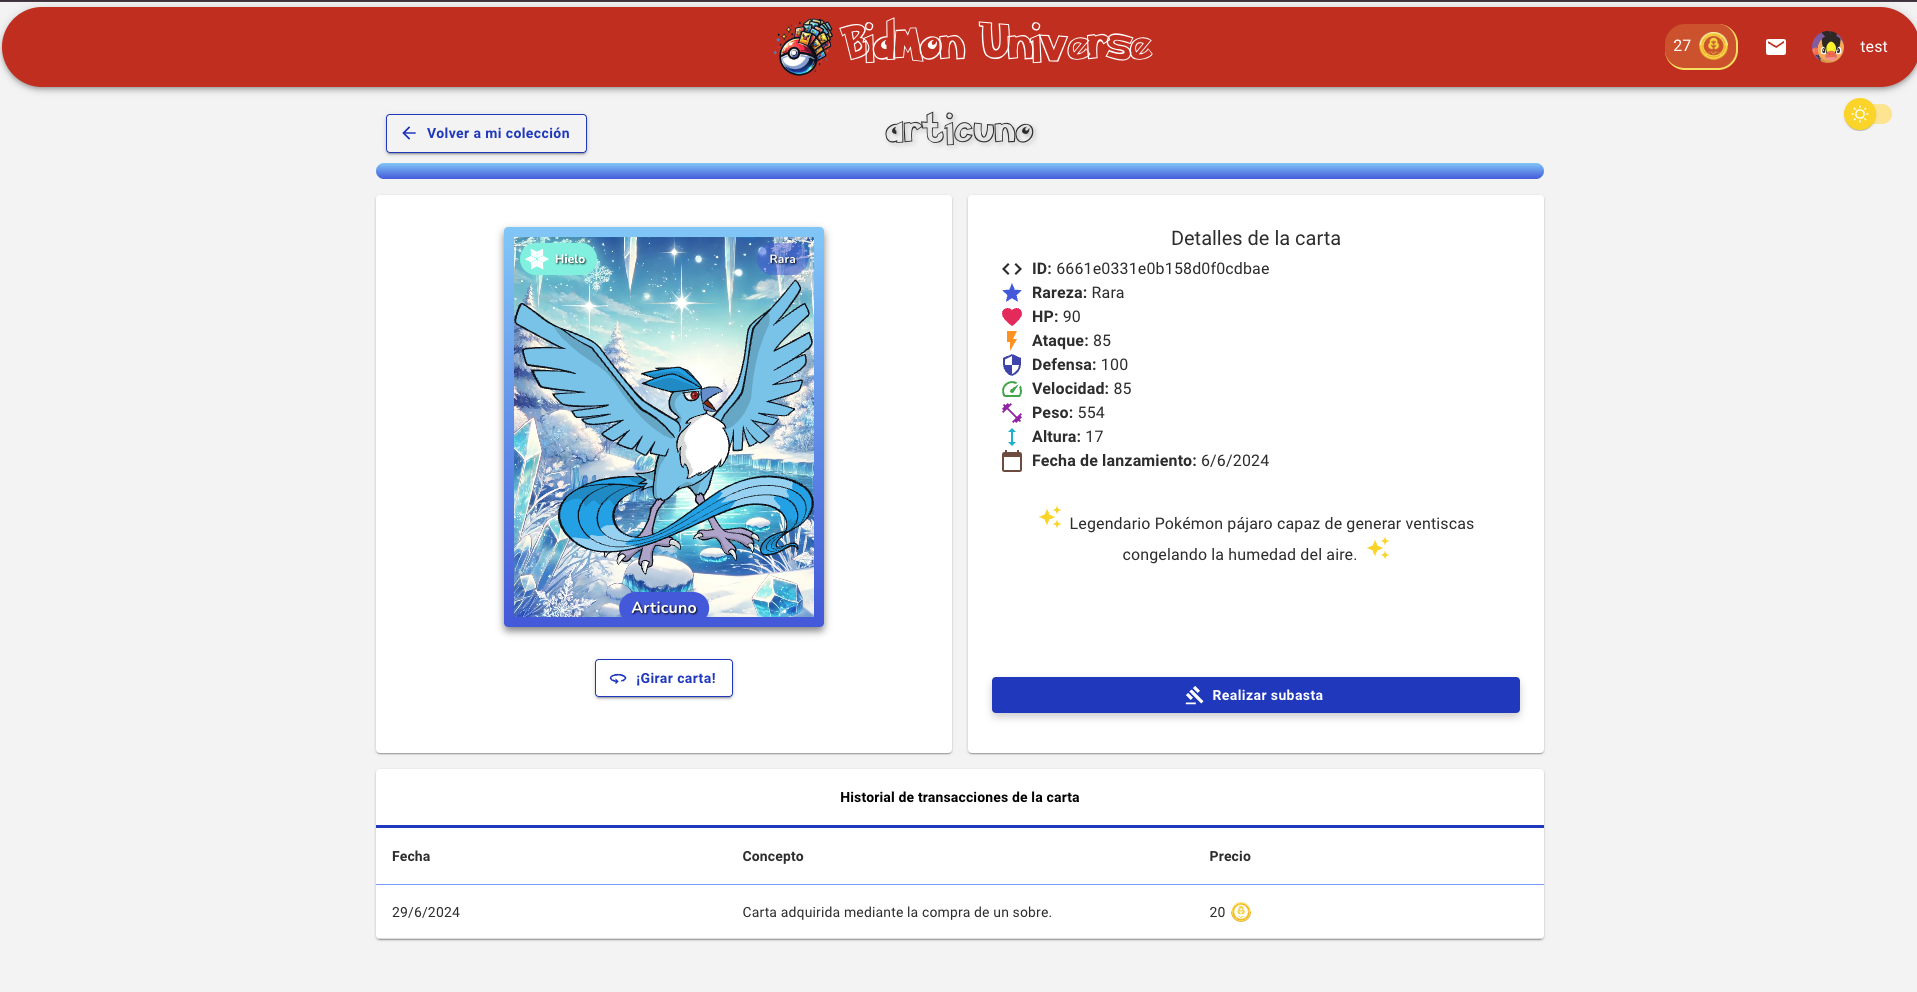
\includegraphics[width=0.8\textwidth]{figures/6-Analisis/6-Interfaz/interfaz/detalle_carta.png}
    \caption{Página de detalle de una carta de la colección del usuario.}
    \label{fig:interfaz-detalle-carta}
\end{figure}


\begin{figure}[H]
    \centering
    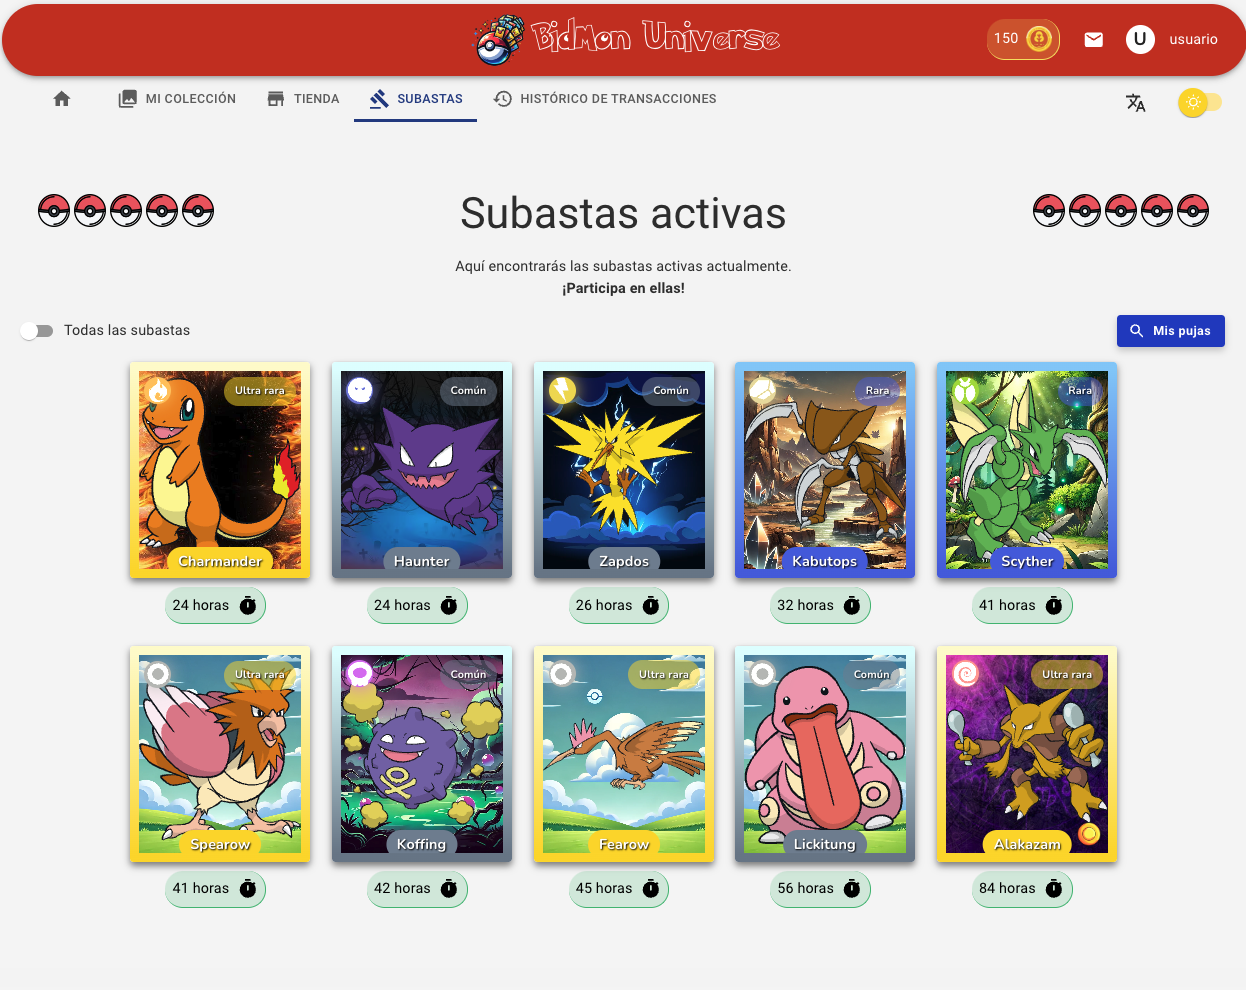
\includegraphics[width=0.8\textwidth]{figures/6-Analisis/6-Interfaz/interfaz/subastas.png}
    \caption{Página de las subastas activas de cartas.}
    \label{fig:interfaz-subastas}
\end{figure}


\begin{figure}[H]
    \centering
    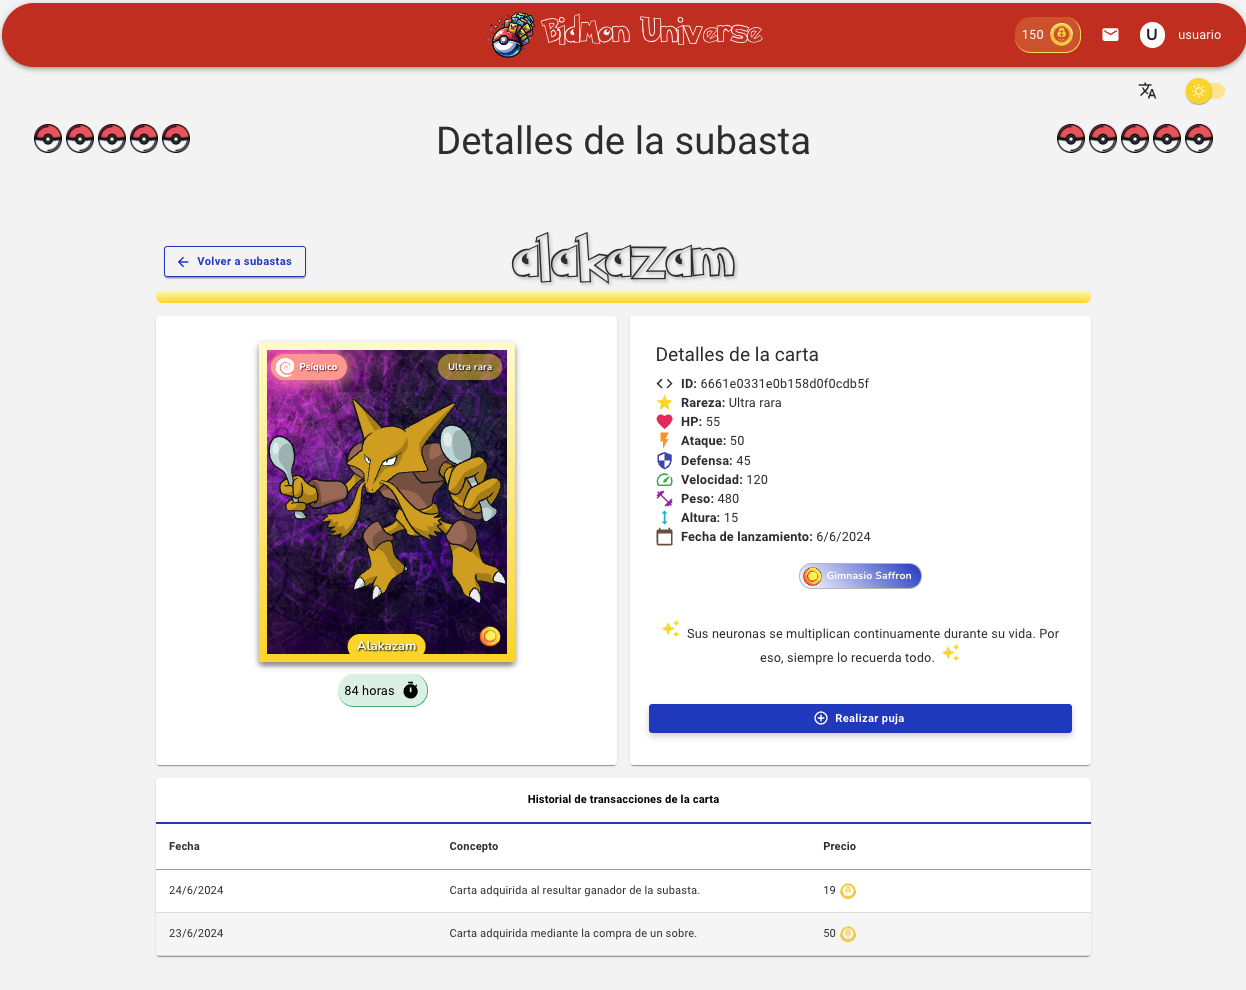
\includegraphics[width=0.8\textwidth]{figures/6-Analisis/6-Interfaz/interfaz/detalle_subasta.png}
    \caption{Página de detalle de una subasta activa.}
    \label{fig:interfaz-detalle-subasta}
\end{figure}

\begin{figure}[H]
    \centering
    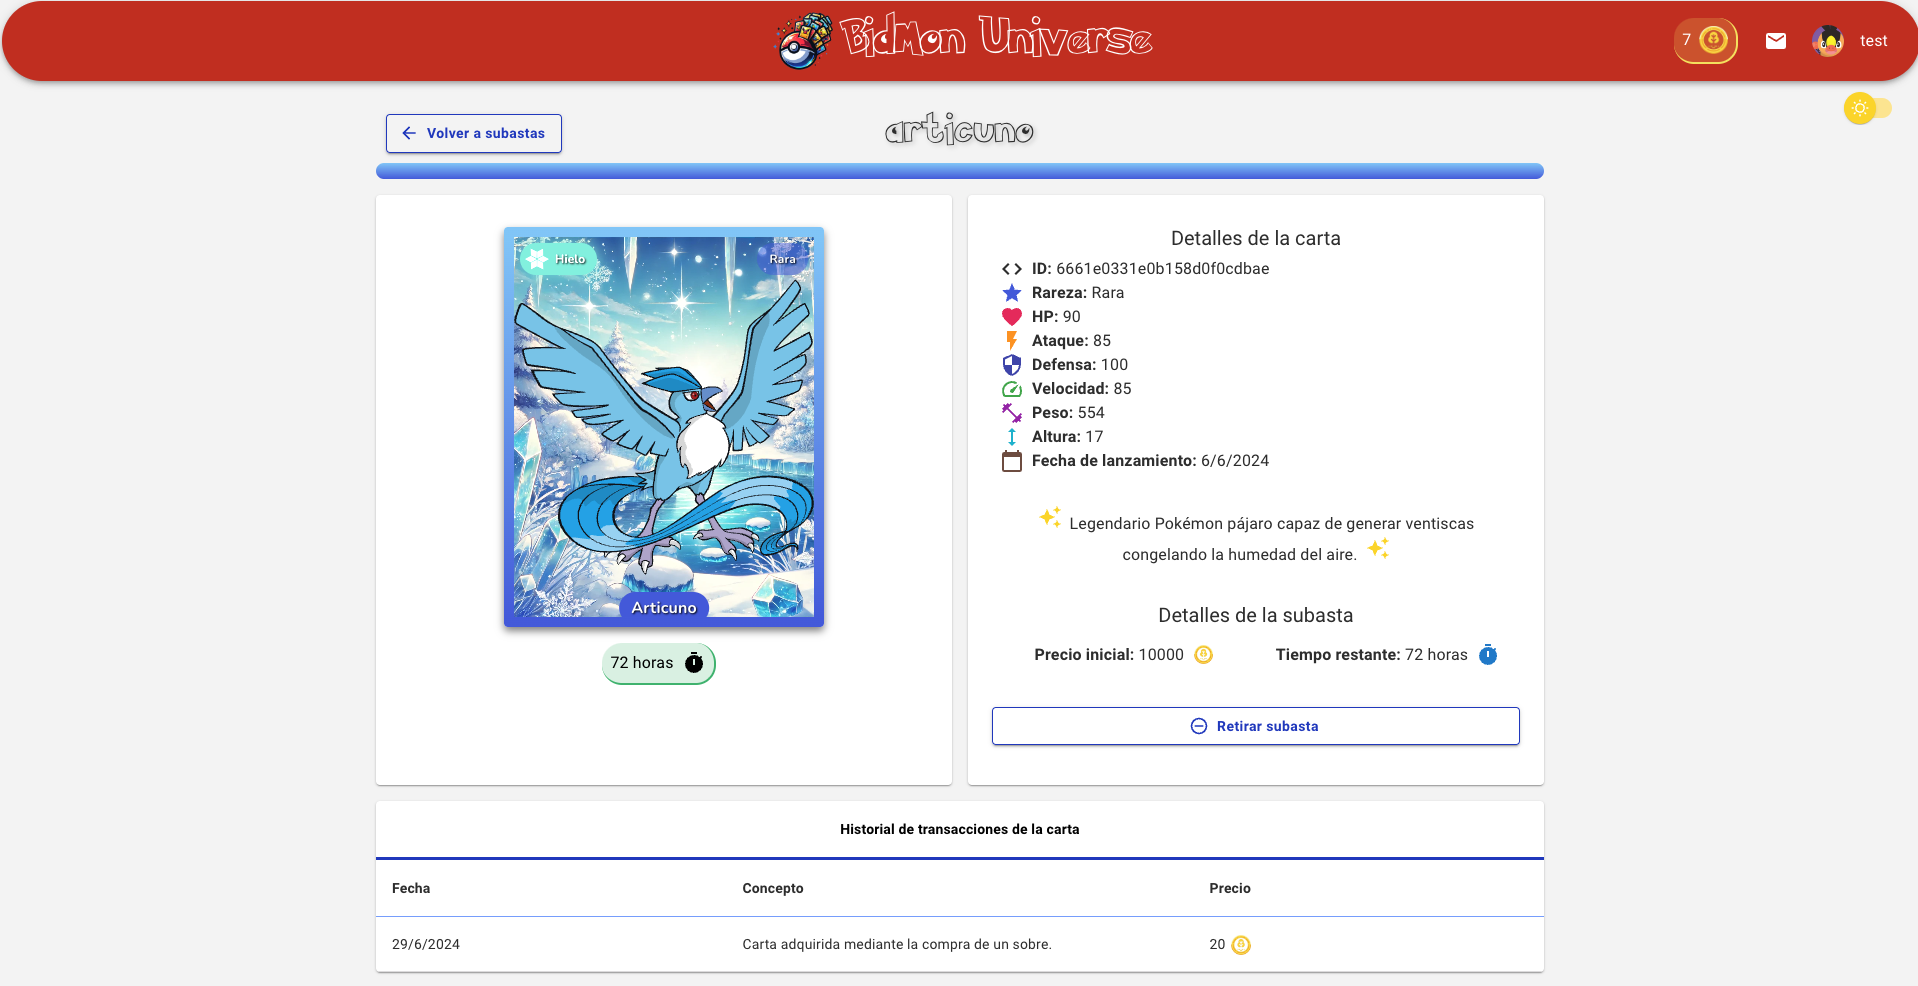
\includegraphics[width=0.8\textwidth]{figures/6-Analisis/6-Interfaz/interfaz/mi_subasta_detalle.png}
    \caption{Página de detalle de una subasta activa creada por el usuario.}
    \label{fig:interfaz-detalle-mi-subasta}
\end{figure}


\begin{figure}[H]
    \centering
    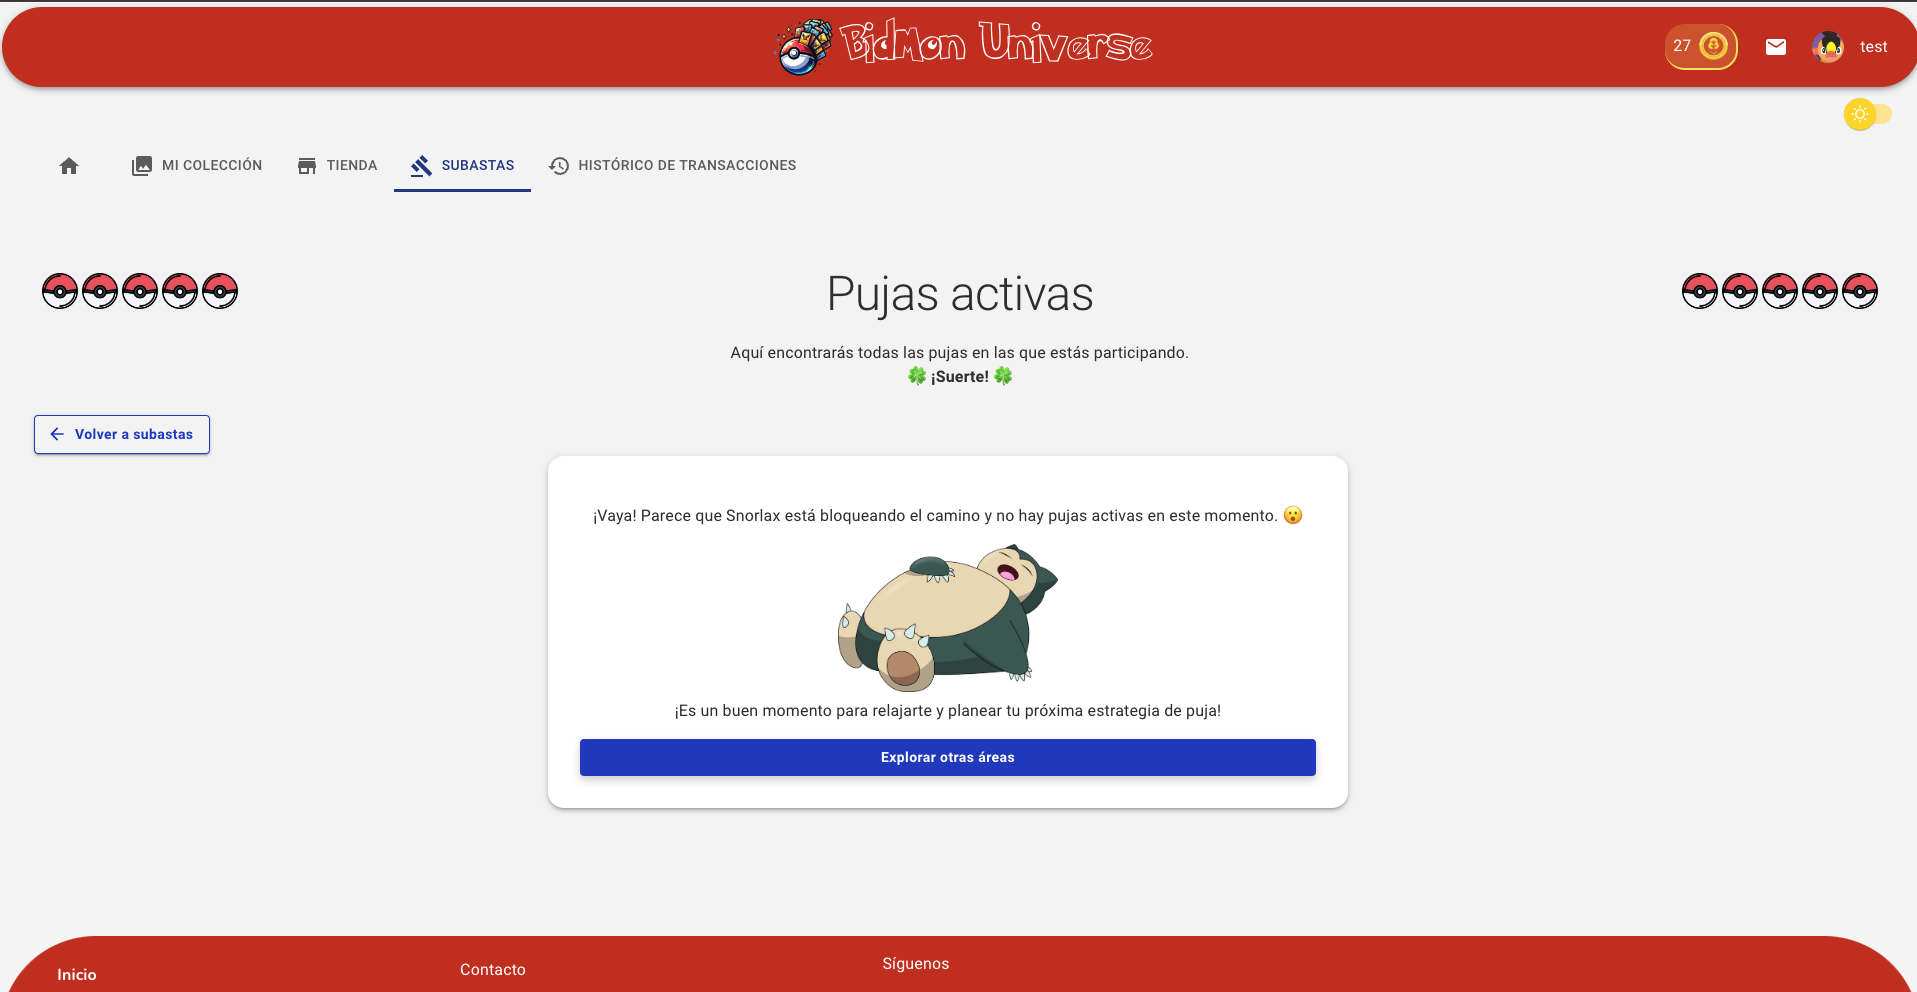
\includegraphics[width=0.8\textwidth]{figures/6-Analisis/6-Interfaz/interfaz/pujas.png}
    \caption{Página de pujas activas del usuario en subastas.}
    \label{fig:interfaz-gimnasios}
\end{figure}


\begin{figure}[H]
    \centering
    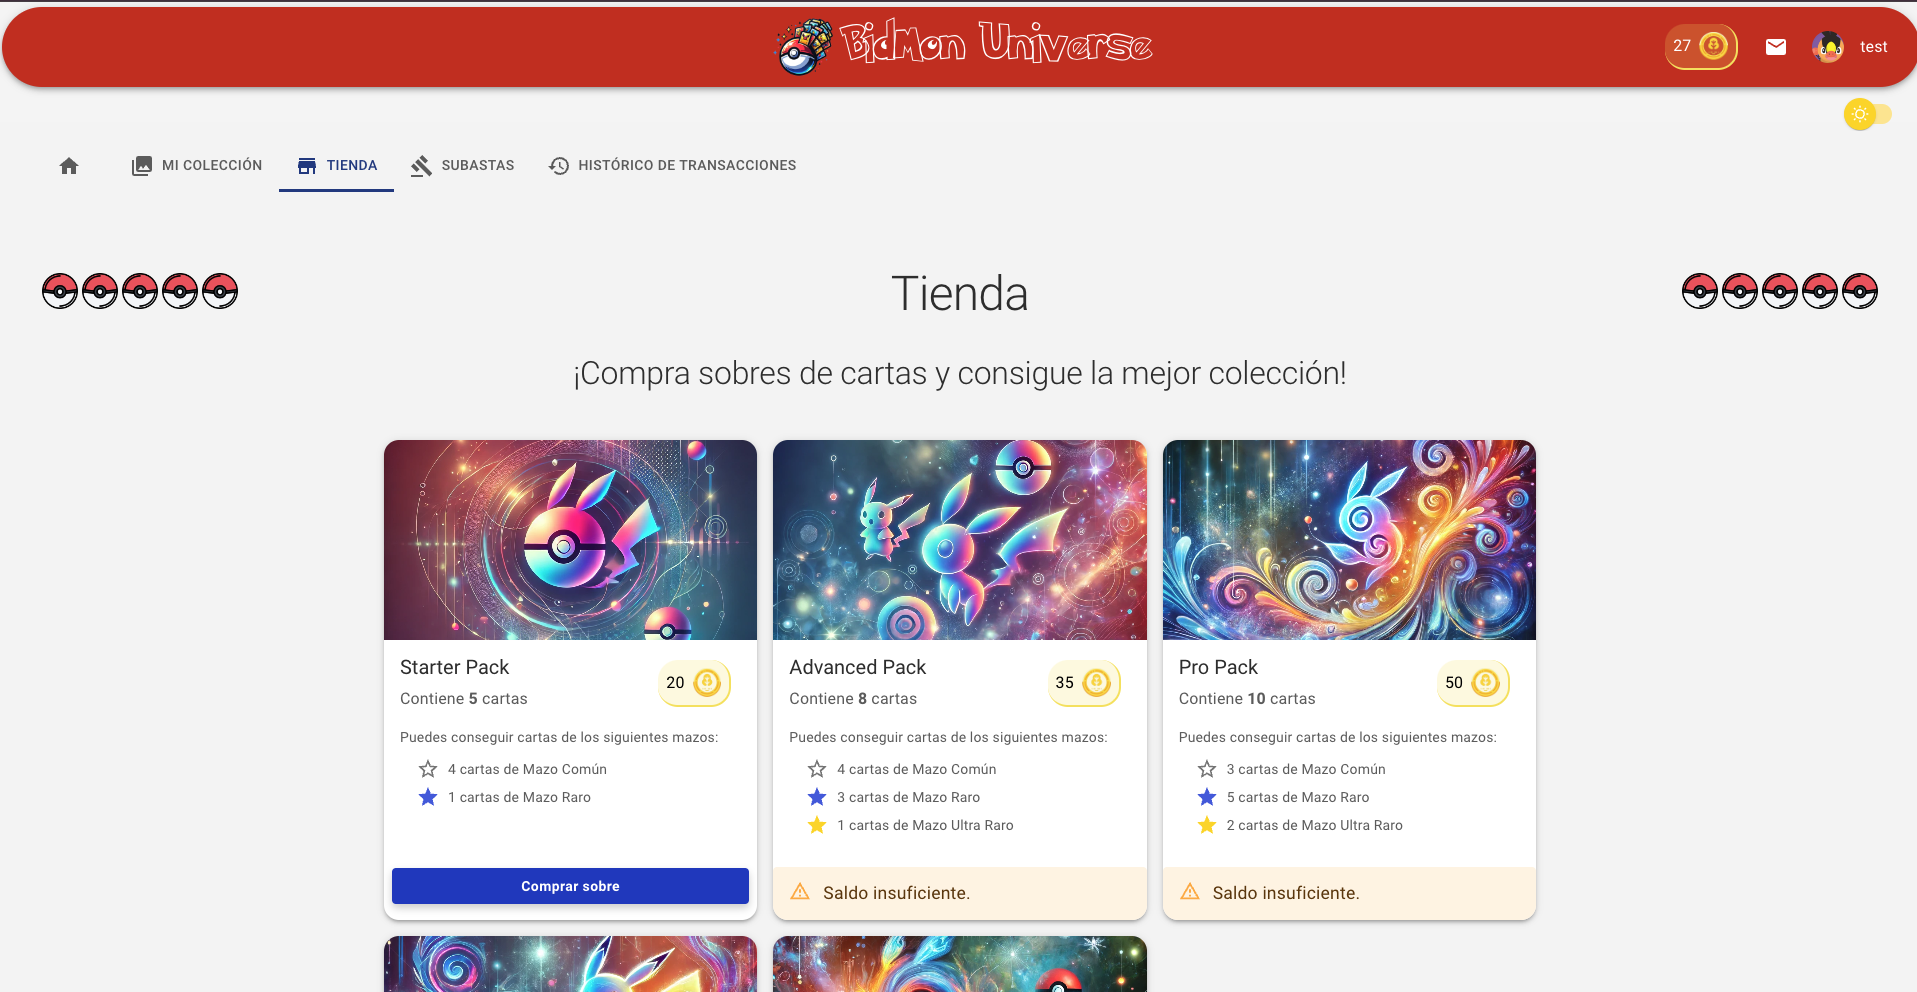
\includegraphics[width=0.8\textwidth]{figures/6-Analisis/6-Interfaz/interfaz/tienda.png}
    \caption{Página de la tienda de sobres de cartas.}
    \label{fig:interfaz-tienda}
\end{figure}


\begin{figure}[H]
    \centering
    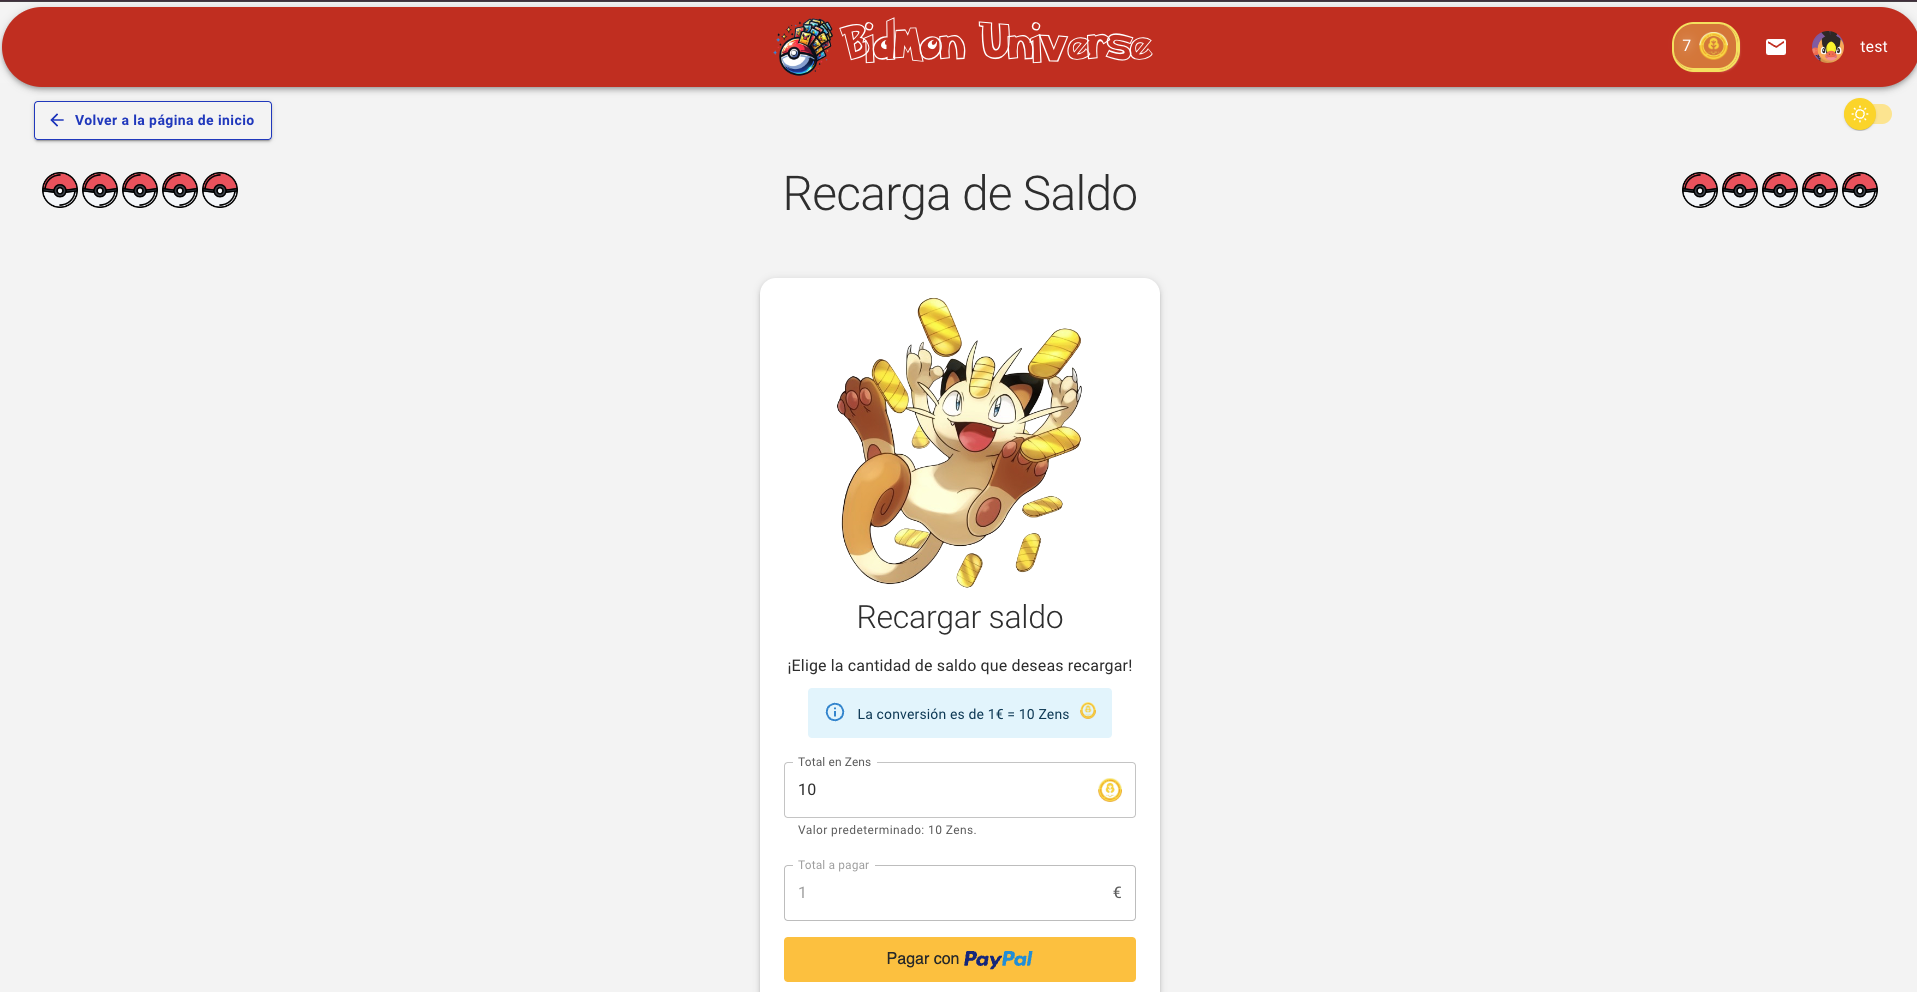
\includegraphics[width=0.8\textwidth]{figures/6-Analisis/6-Interfaz/interfaz/recarga.png}
    \caption{Página de recarga de saldo de la aplicación.}
    \label{fig:interfaz-recarga}
\end{figure}


\begin{figure}[H]
    \centering
    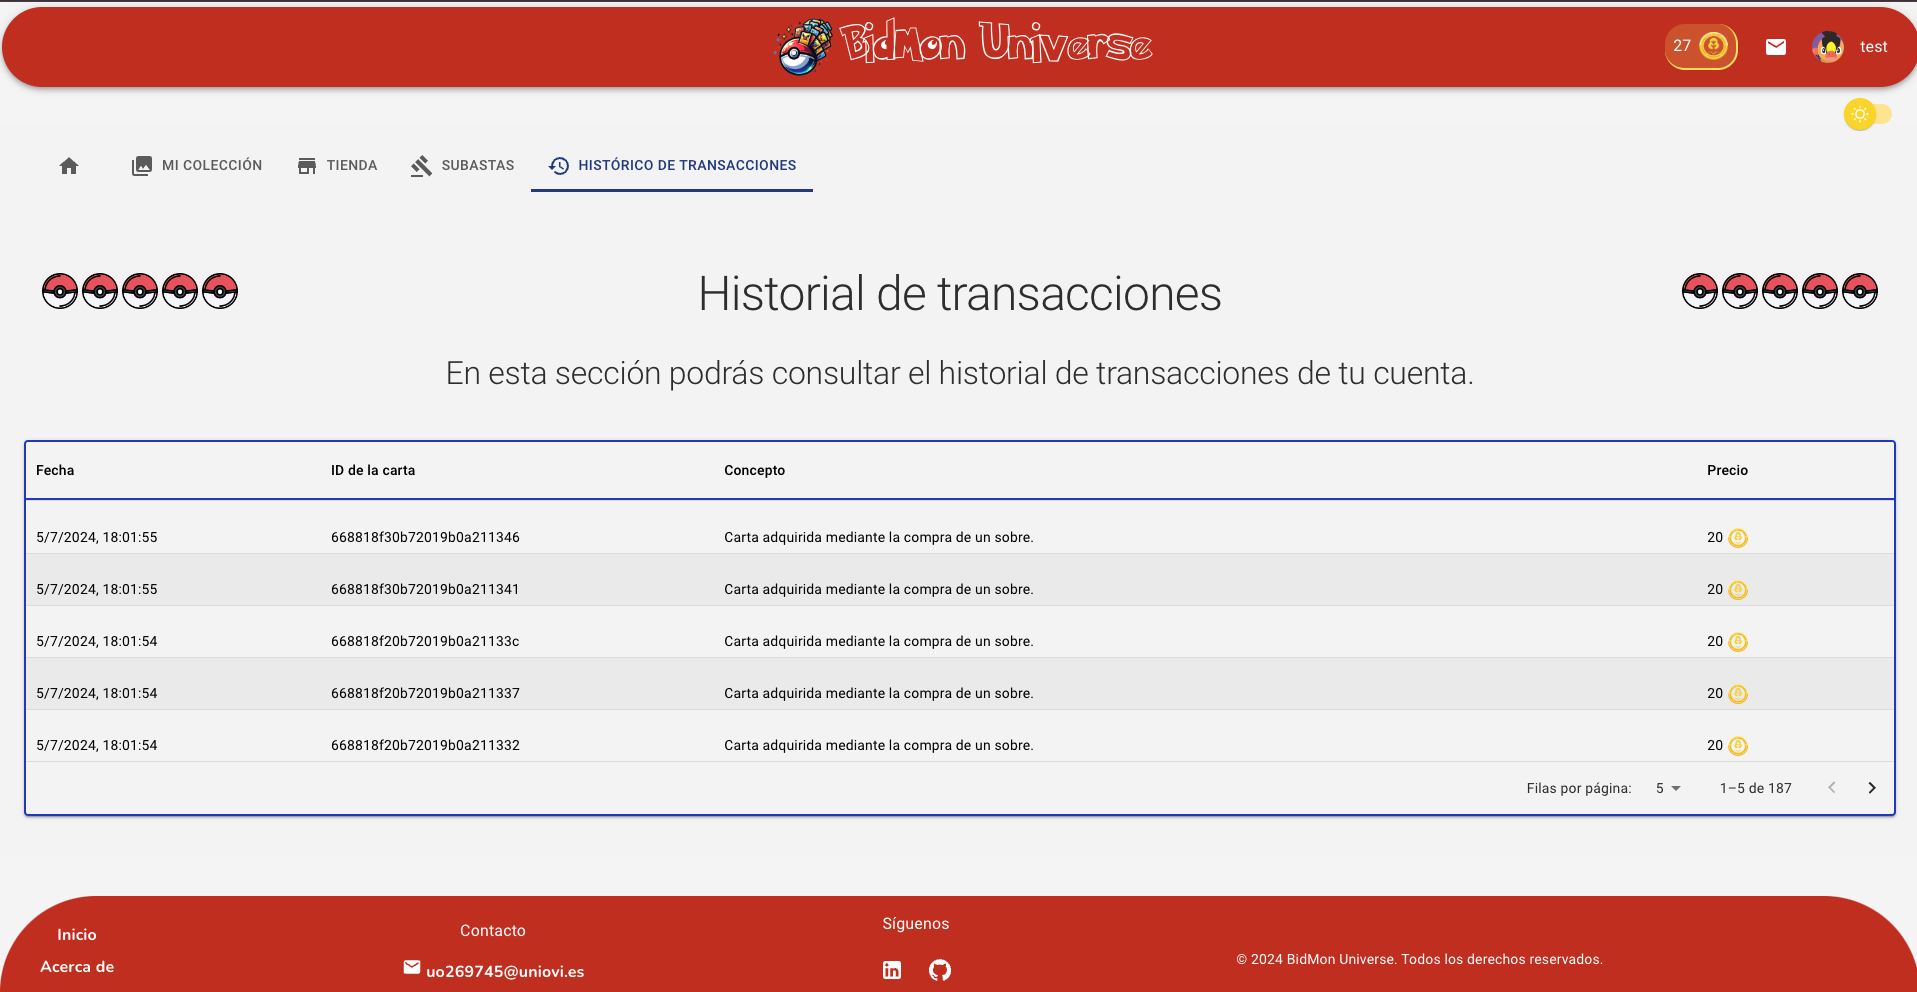
\includegraphics[width=0.8\textwidth]{figures/6-Analisis/6-Interfaz/interfaz/transacciones.png}
    \caption{Página de transacciones realizadas por el usuario.}
    \label{fig:interfaz-transacciones}
\end{figure}

\begin{figure}[H]
    \centering
    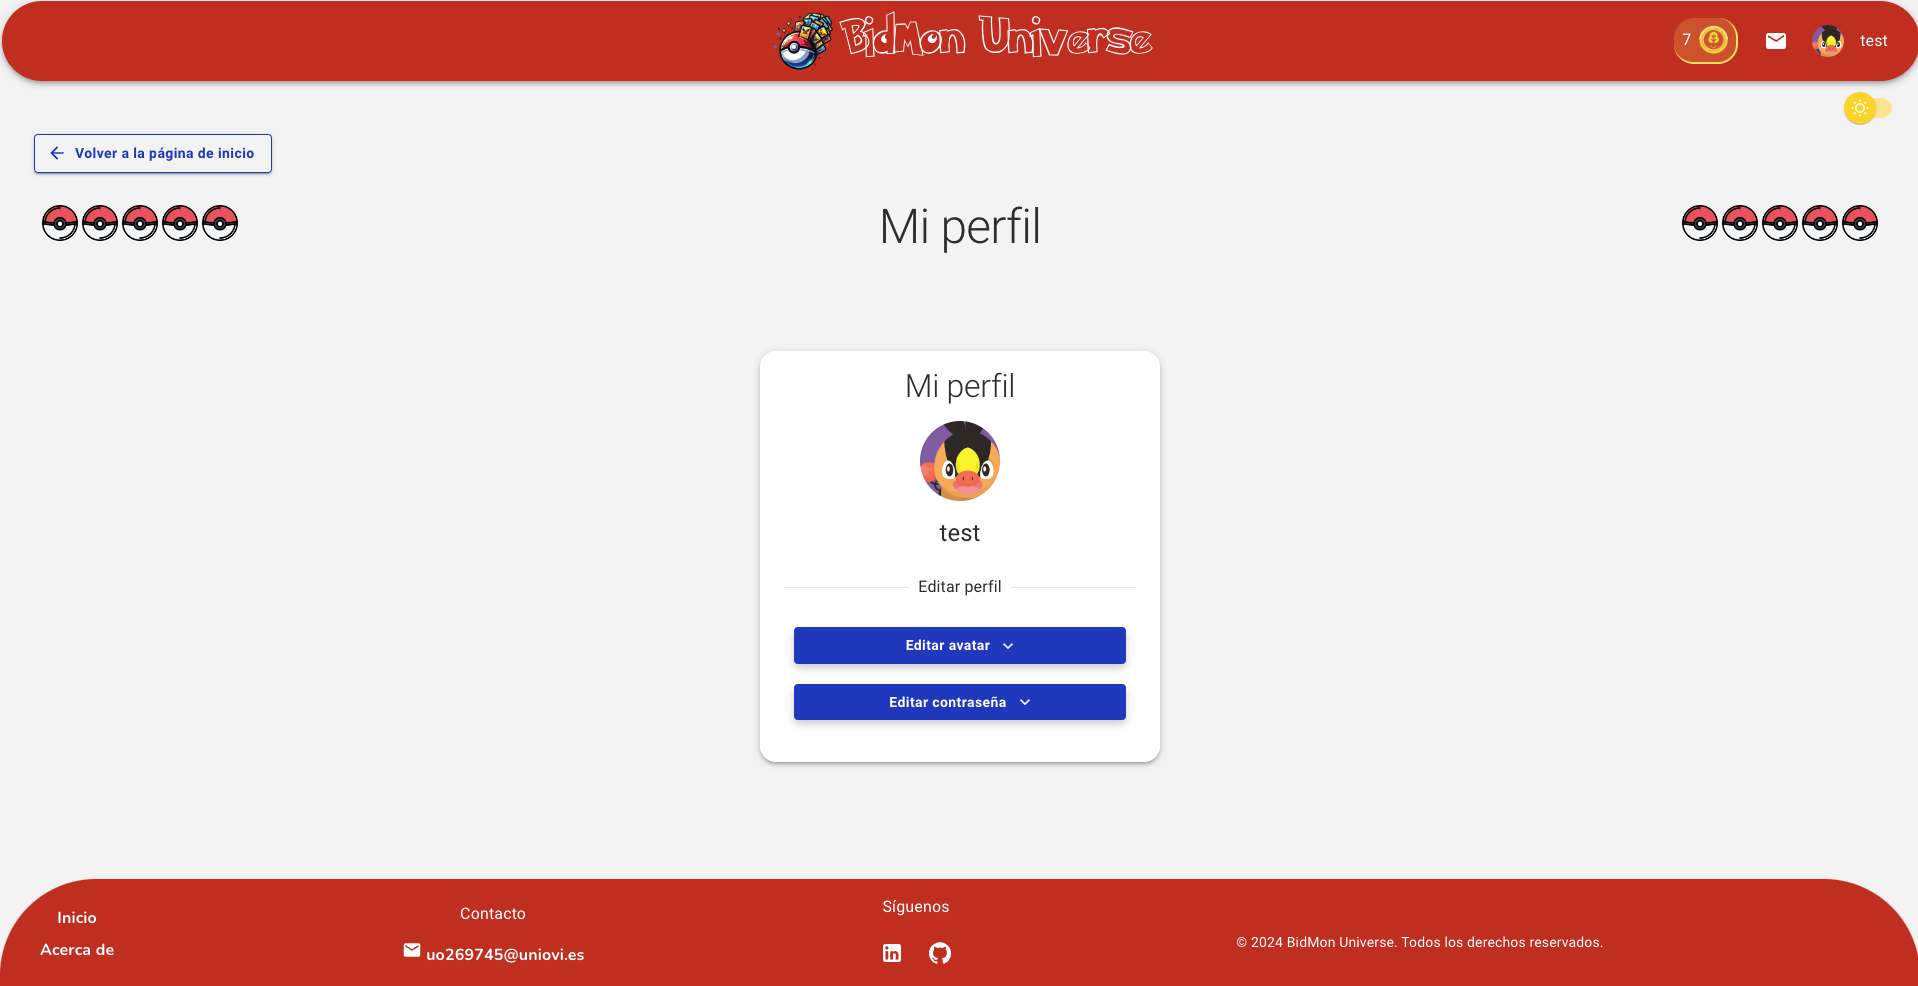
\includegraphics[width=0.8\textwidth]{figures/6-Analisis/6-Interfaz/interfaz/perfil1.png}
    \caption{Página de perfil del usuario.}
    \label{fig:interfaz-perfil1}
\end{figure}


\begin{figure}[H]
    \centering
    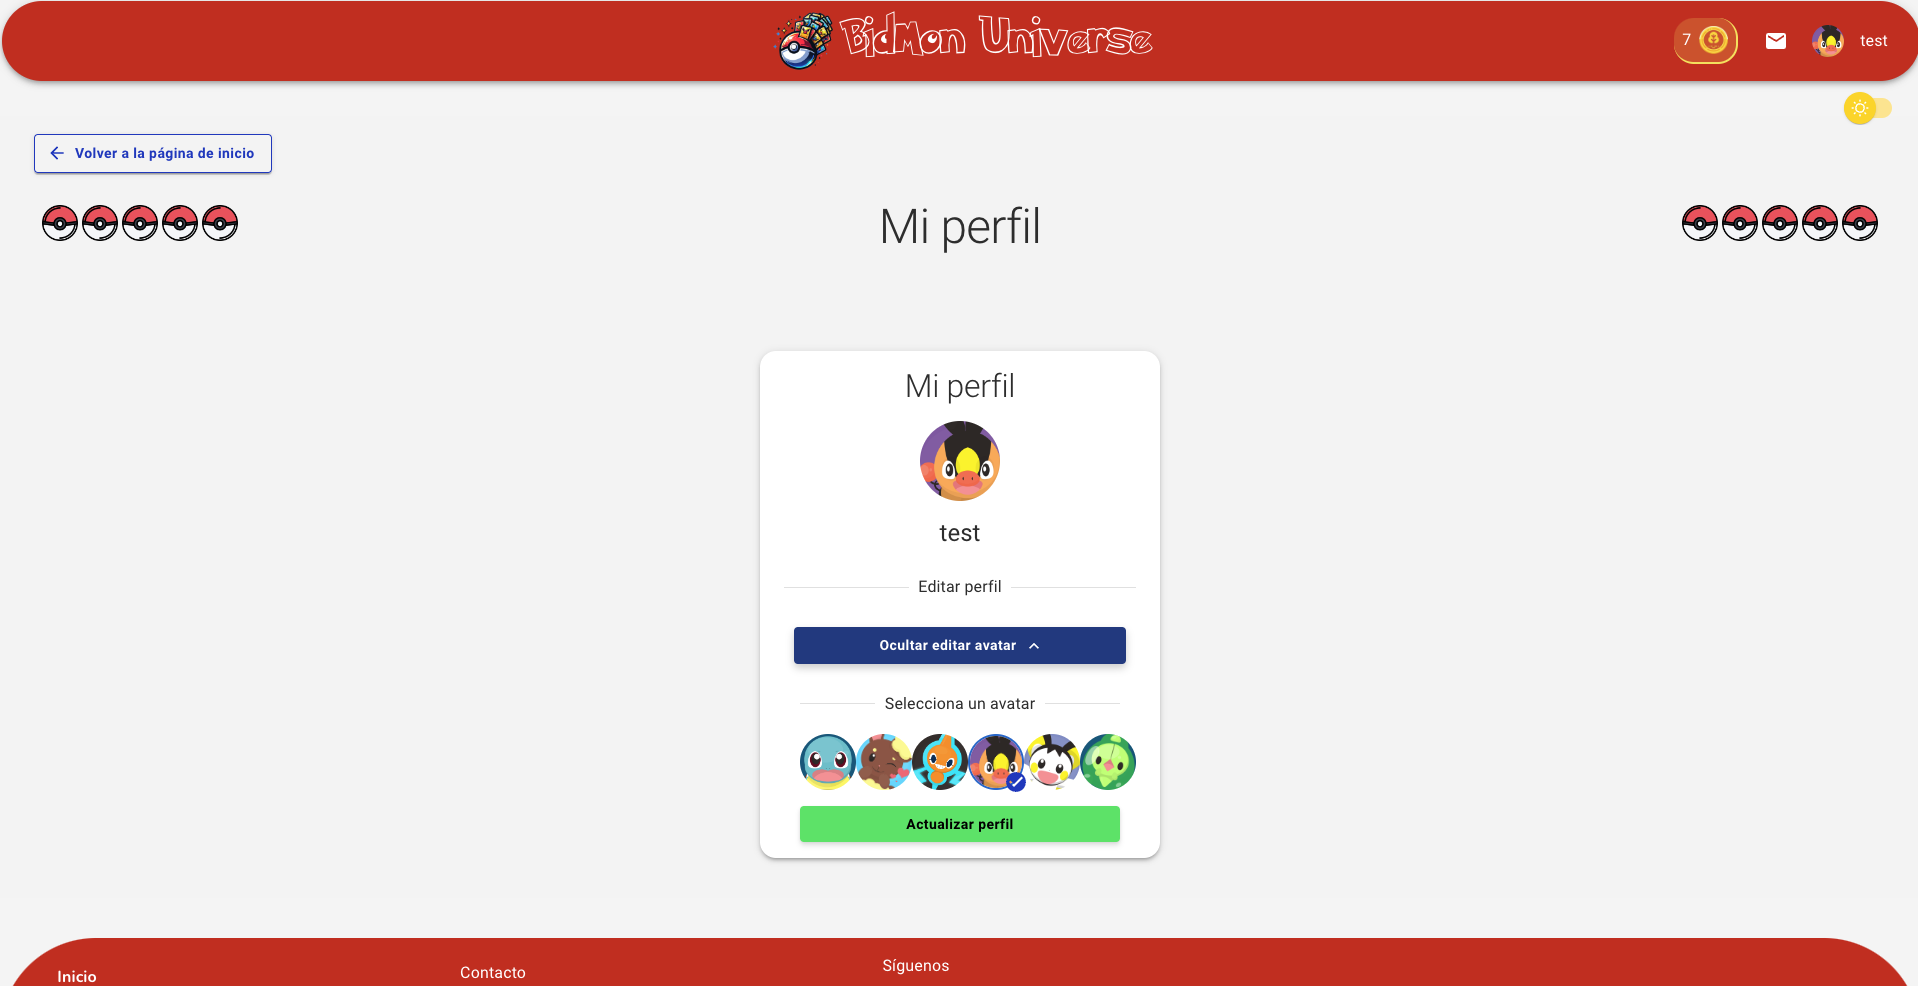
\includegraphics[width=0.8\textwidth]{figures/6-Analisis/6-Interfaz/interfaz/perfil2.png}
    \caption{Página de perfil del usuario, con la opción de cambiar la imagen de perfil desplegada.}
    \label{fig:interfaz-perfil2}
\end{figure}


\begin{figure}[H]
    \centering
    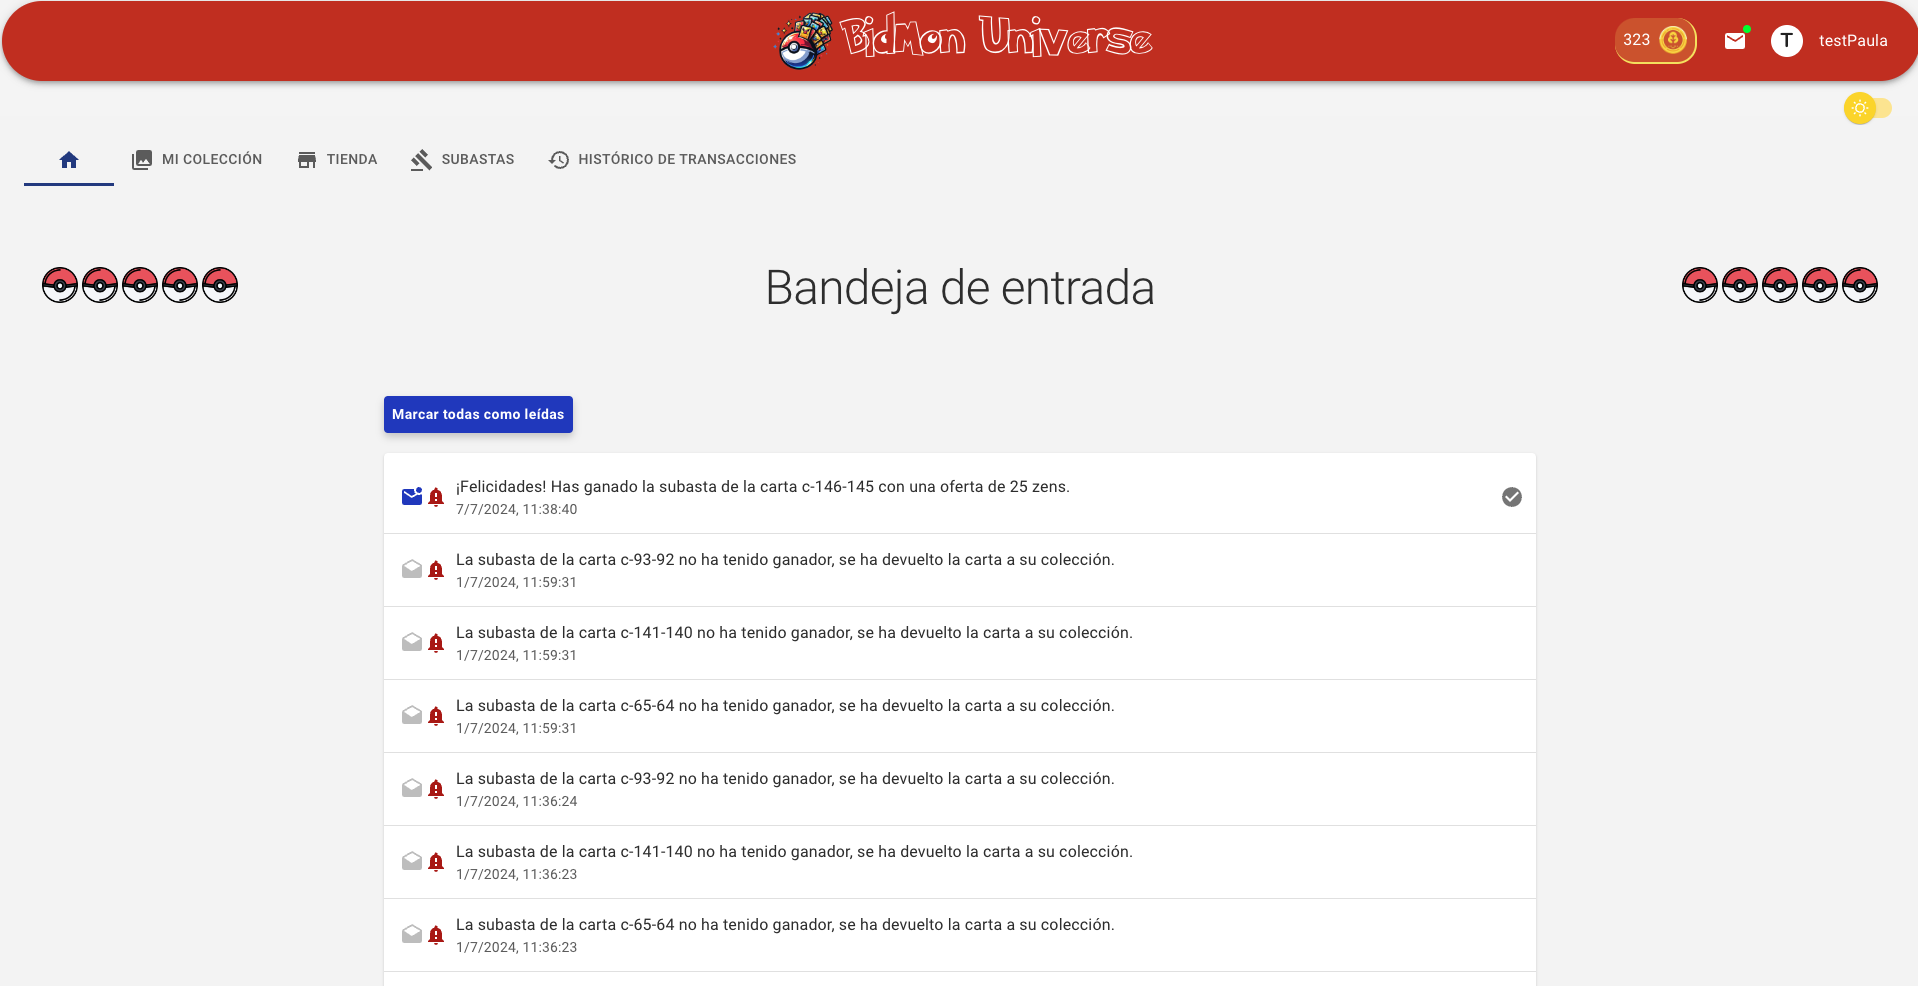
\includegraphics[width=0.8\textwidth]{figures/6-Analisis/6-Interfaz/interfaz/notificaciones_2.png}
    \caption{Página de notificaciones del usuario.}
    \label{fig:interfaz-notificaciones}
\end{figure}


El usuario puede elegir entre dos temas de la aplicación: el tema claro y el tema oscuro.
El tema claro es el que se muestra en las imágenes anteriores.
A continuación se adjuntan un par de imágenes de la aplicación en el tema oscuro, la página de inicio
y la página de pujas activas del usuario.

\begin{figure}[H]
    \centering
    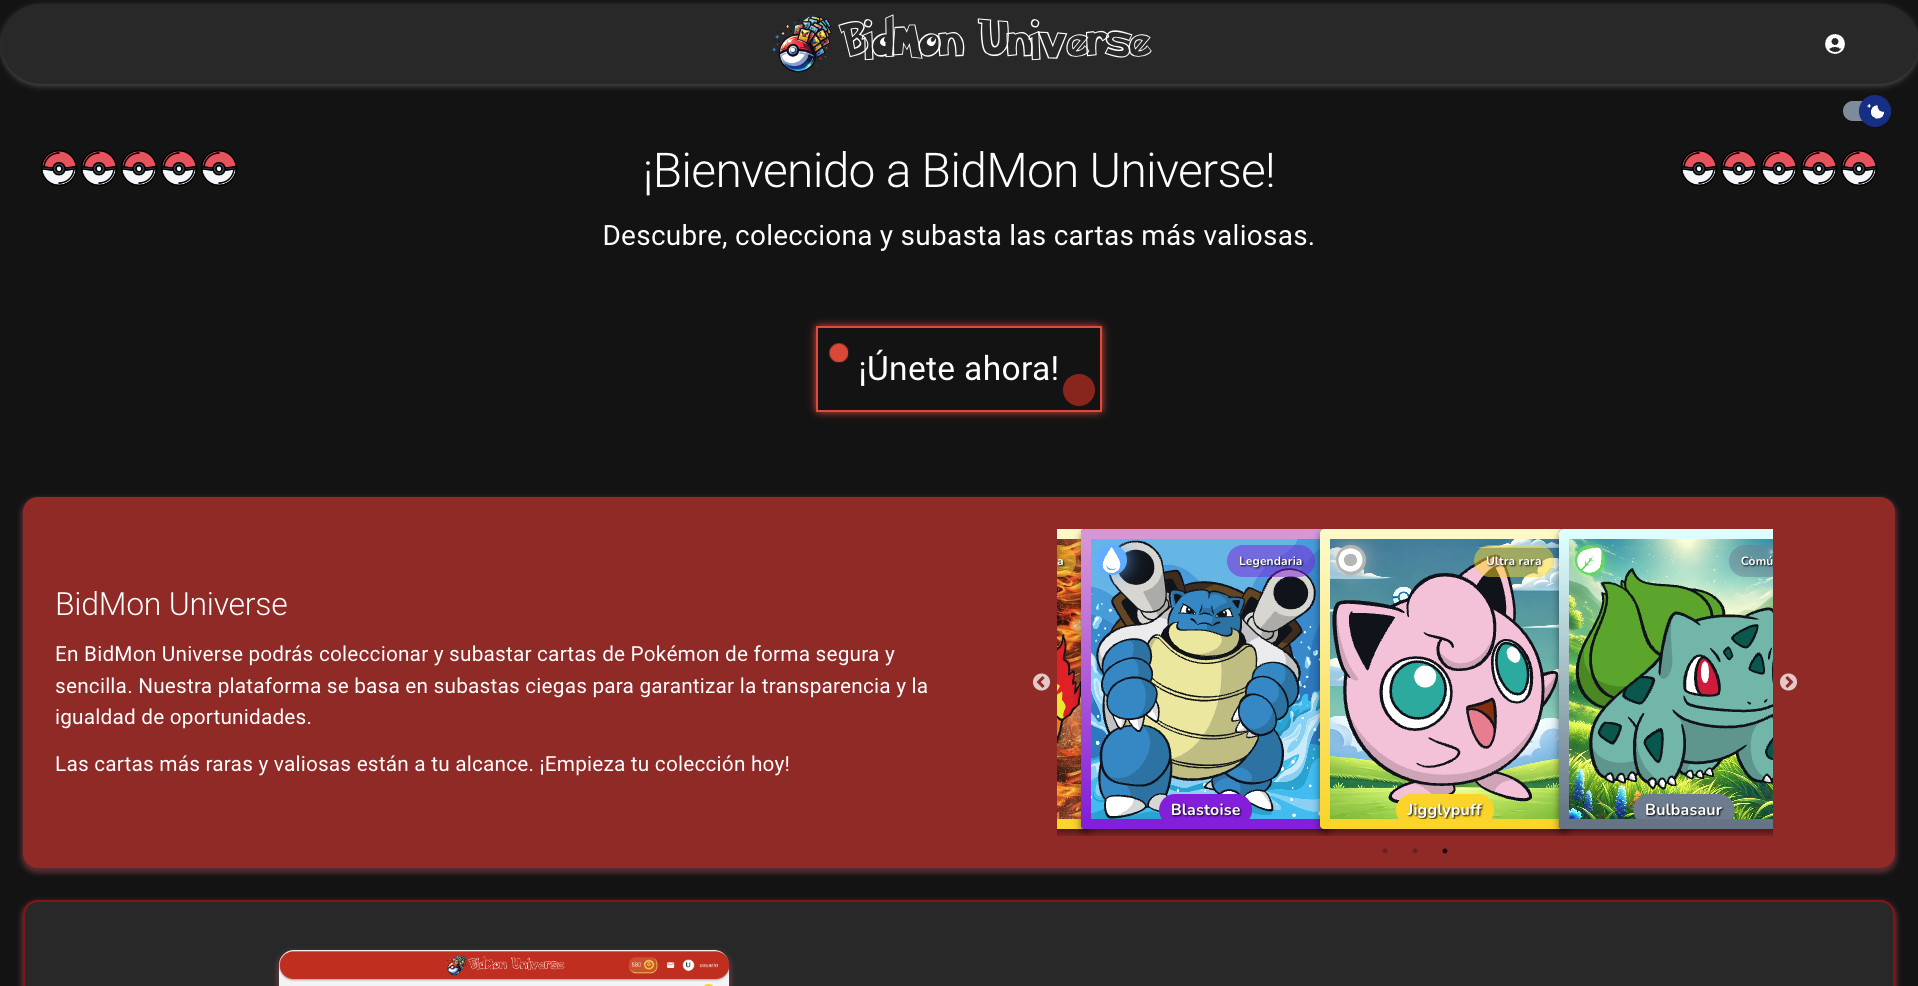
\includegraphics[width=0.8\textwidth]{figures/6-Analisis/6-Interfaz/interfaz/home_dark.png}
    \caption{Página Home en tema oscuro.}
    \label{fig:interfaz-home-dark}
\end{figure}

\begin{figure}[H]
    \centering
    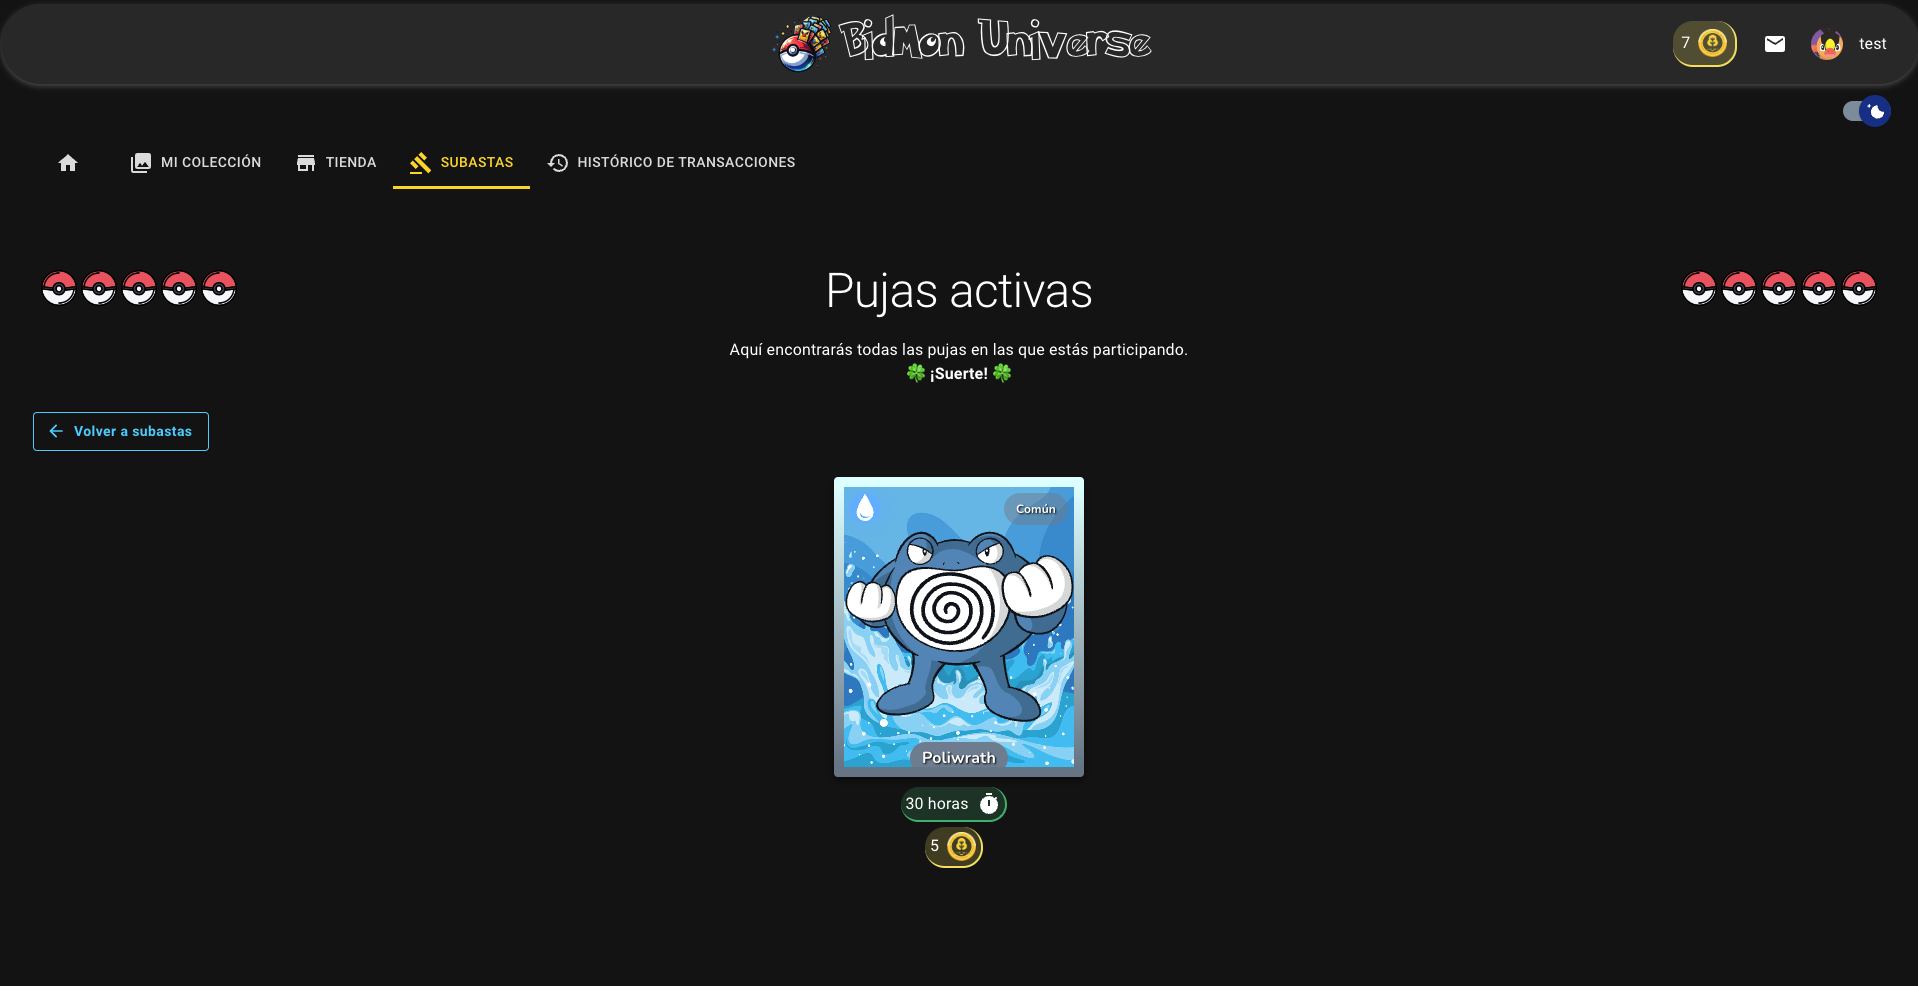
\includegraphics[width=0.8\textwidth]{figures/6-Analisis/6-Interfaz/interfaz/pujas_dark.png}
    \caption{Página de pujas activas del usuario en tema oscuro.}
    \label{fig:interfaz-pujas-dark}
\end{figure}

\subsection{Descripción del Comportamiento de la Interfaz} 
La interacción con la interfaz es sencilla,
los botones tienen dos funcionalidades principales que son la de redirigir a otra página o la de realizar una acción.

Esta acción puede ser la de abrir un modal, como en el caso de la subasta de una carta o un menú desplegable, como en el caso del menú de usuario.

Los comportamientos más complejos de la interfaz son los de la subasta de una carta y la compra de un sobre de cartas.
Estos comportamientos se han diseñado de forma que sean intuitivos y fáciles de entender para el usuario.

A continuación, se mostrará un ejemplo de cada uno de estos comportamientos.

\subsubsection{Subasta de una carta}
En la \coloredUnderline{\hyperlink{fig:interfaz-subasta}{Figura \ref*{fig:interfaz-subasta}}} se muestra la vista del modal de crear una subasta.
En esta vista, el usuario puede seleccionar el precio de salida de la carta y el tiempo que durará la subasta.

\begin{figure}[H]
    \centering
    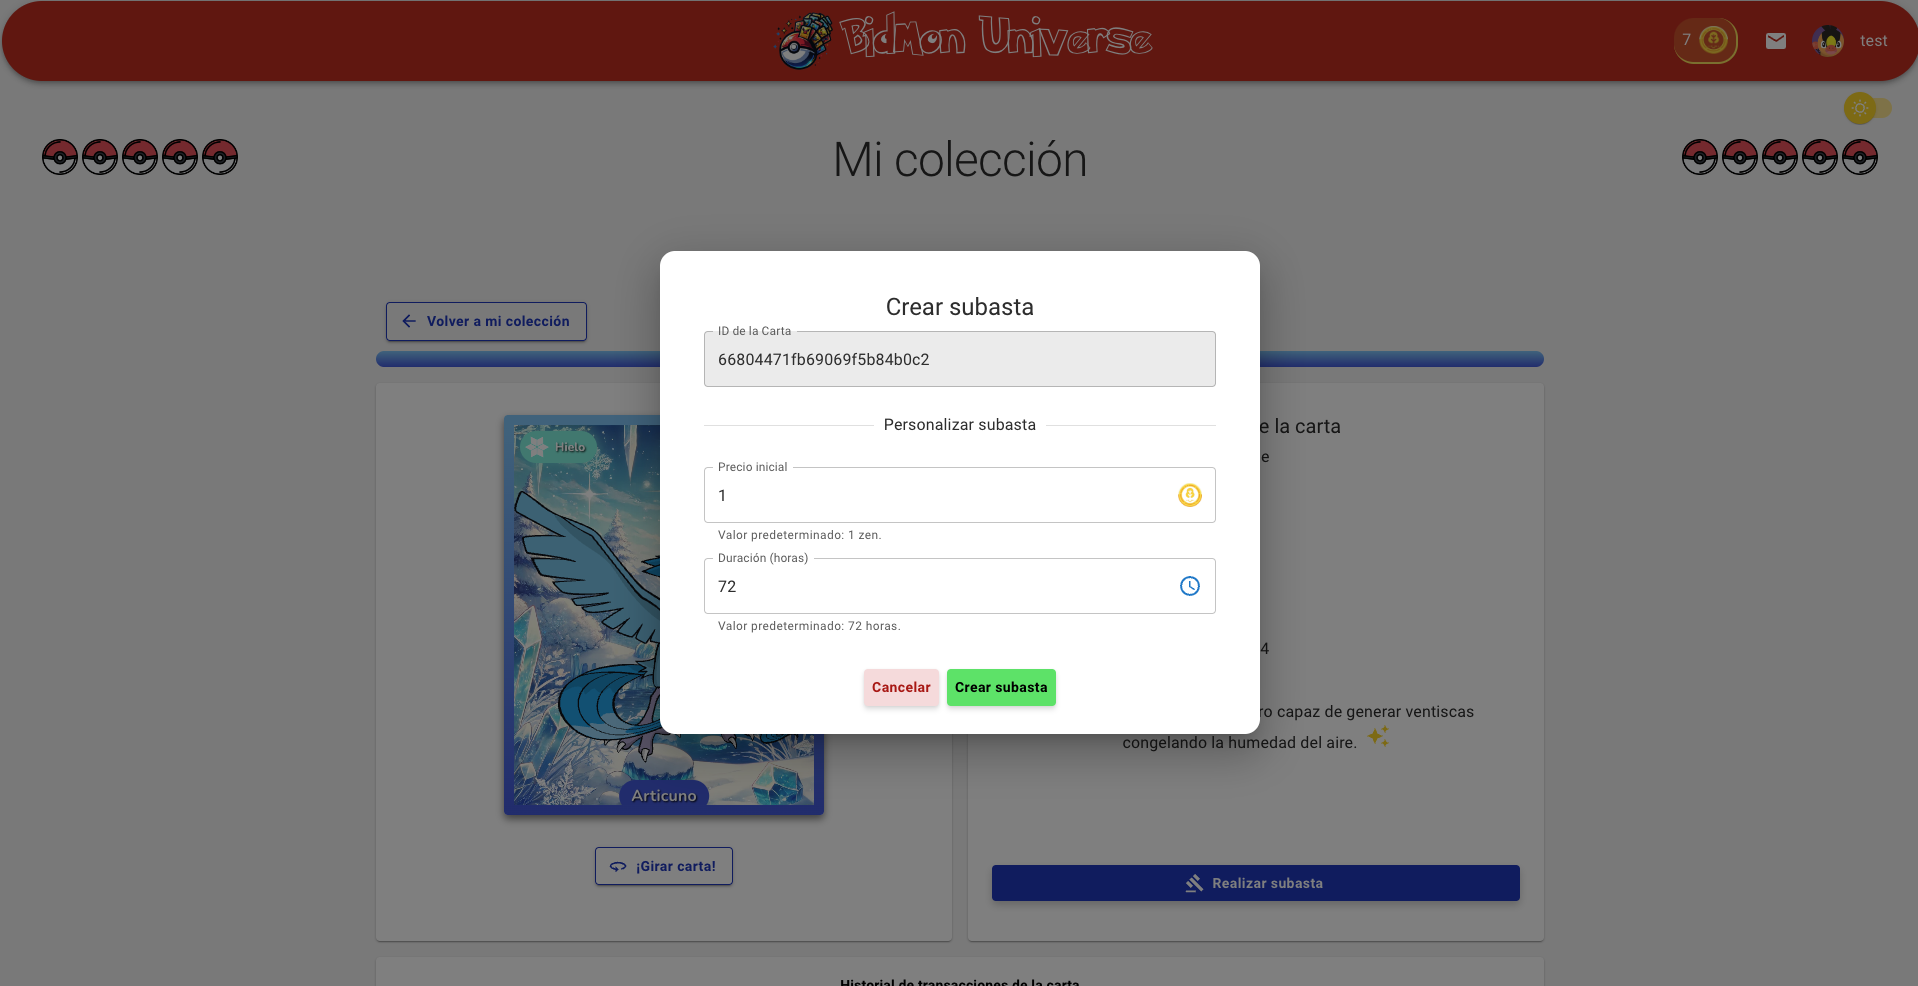
\includegraphics[width=0.8\textwidth]{figures/6-Analisis/6-Interfaz/interfaz/crear-subasta1.png}
    \caption{Modal de creación de subasta.}
    \hypertarget{fig:interfaz-subasta}{}
    \label{fig:interfaz-subasta}
\end{figure}

Una vez que el usuario ha rellenado los campos, puede pulsar el botón de \textit{Crear subasta} para confirmar la subasta.
Se le abrirá un modal de confirmación, en el que se le mostrará un resumen de la subasta y podrá confirmarla o cancelarla.

\begin{figure}[H]
    \centering
    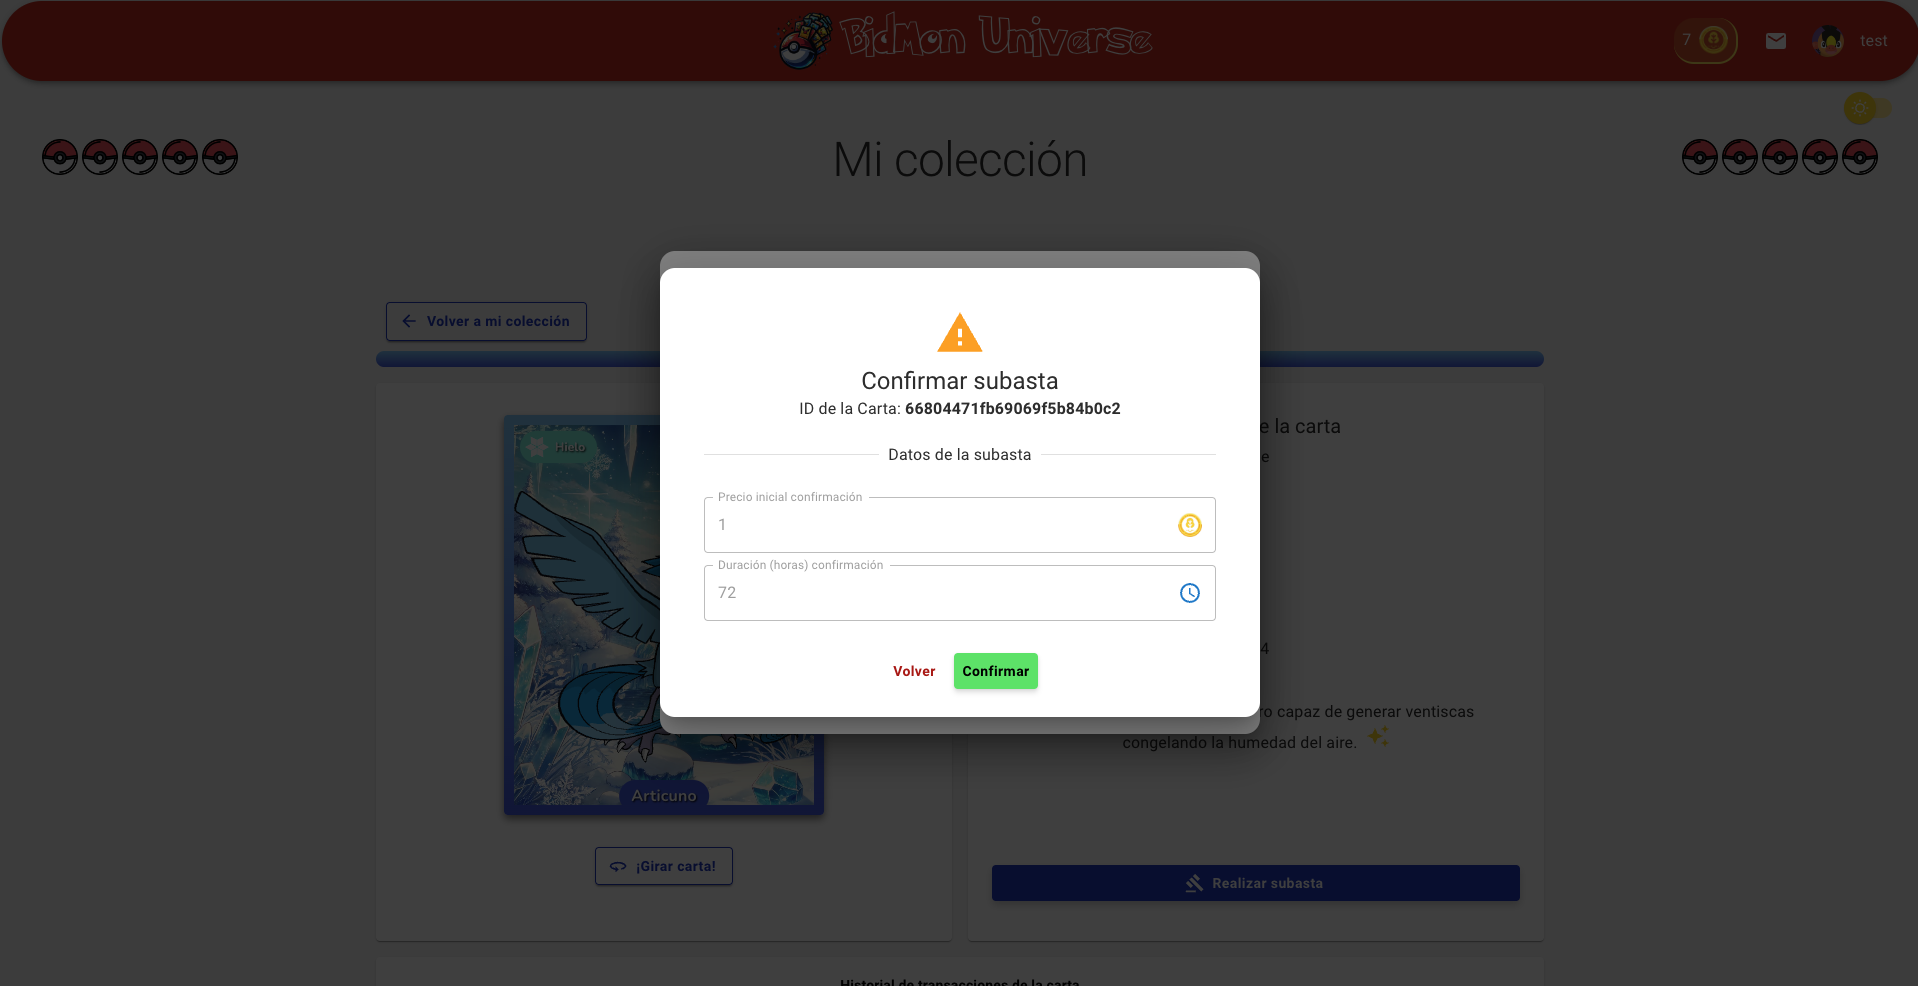
\includegraphics[width=0.8\textwidth]{figures/6-Analisis/6-Interfaz/interfaz/crear-subasta2.png}
    \caption{Modal de confirmación de subasta.}
    \label{fig:interfaz-subasta-alerta}
\end{figure}

Si confirma la subasta, se mostrará un mensaje de éxito, se cerrará el modal y desparecerá el botón de subastar reemplazándolo por una
alerta informativa de que la carta está en subasta.

\begin{figure}[H]
    \centering
    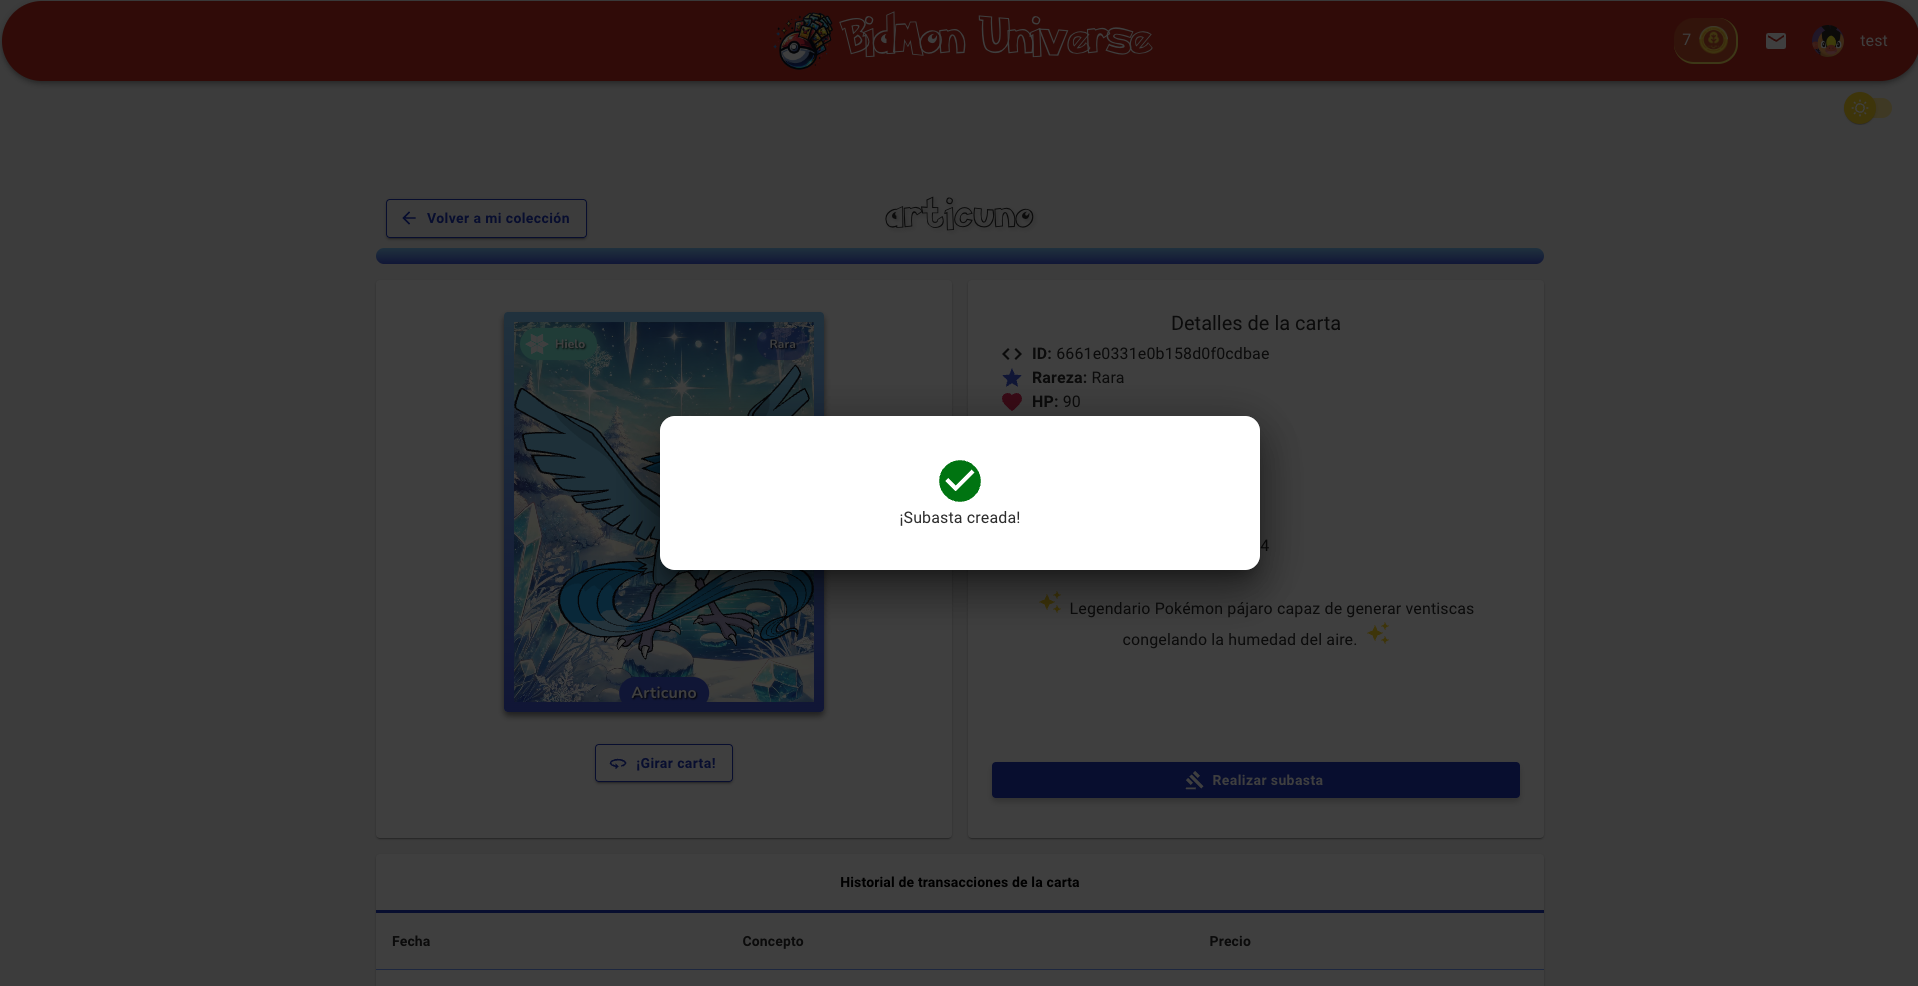
\includegraphics[width=0.8\textwidth]{figures/6-Analisis/6-Interfaz/interfaz/subasta_creada.png}
    \caption{Mensaje de éxito de creación de subasta.}
    \label{fig:interfaz-subasta-exito}
\end{figure}

\begin{figure}[H]
    \centering
    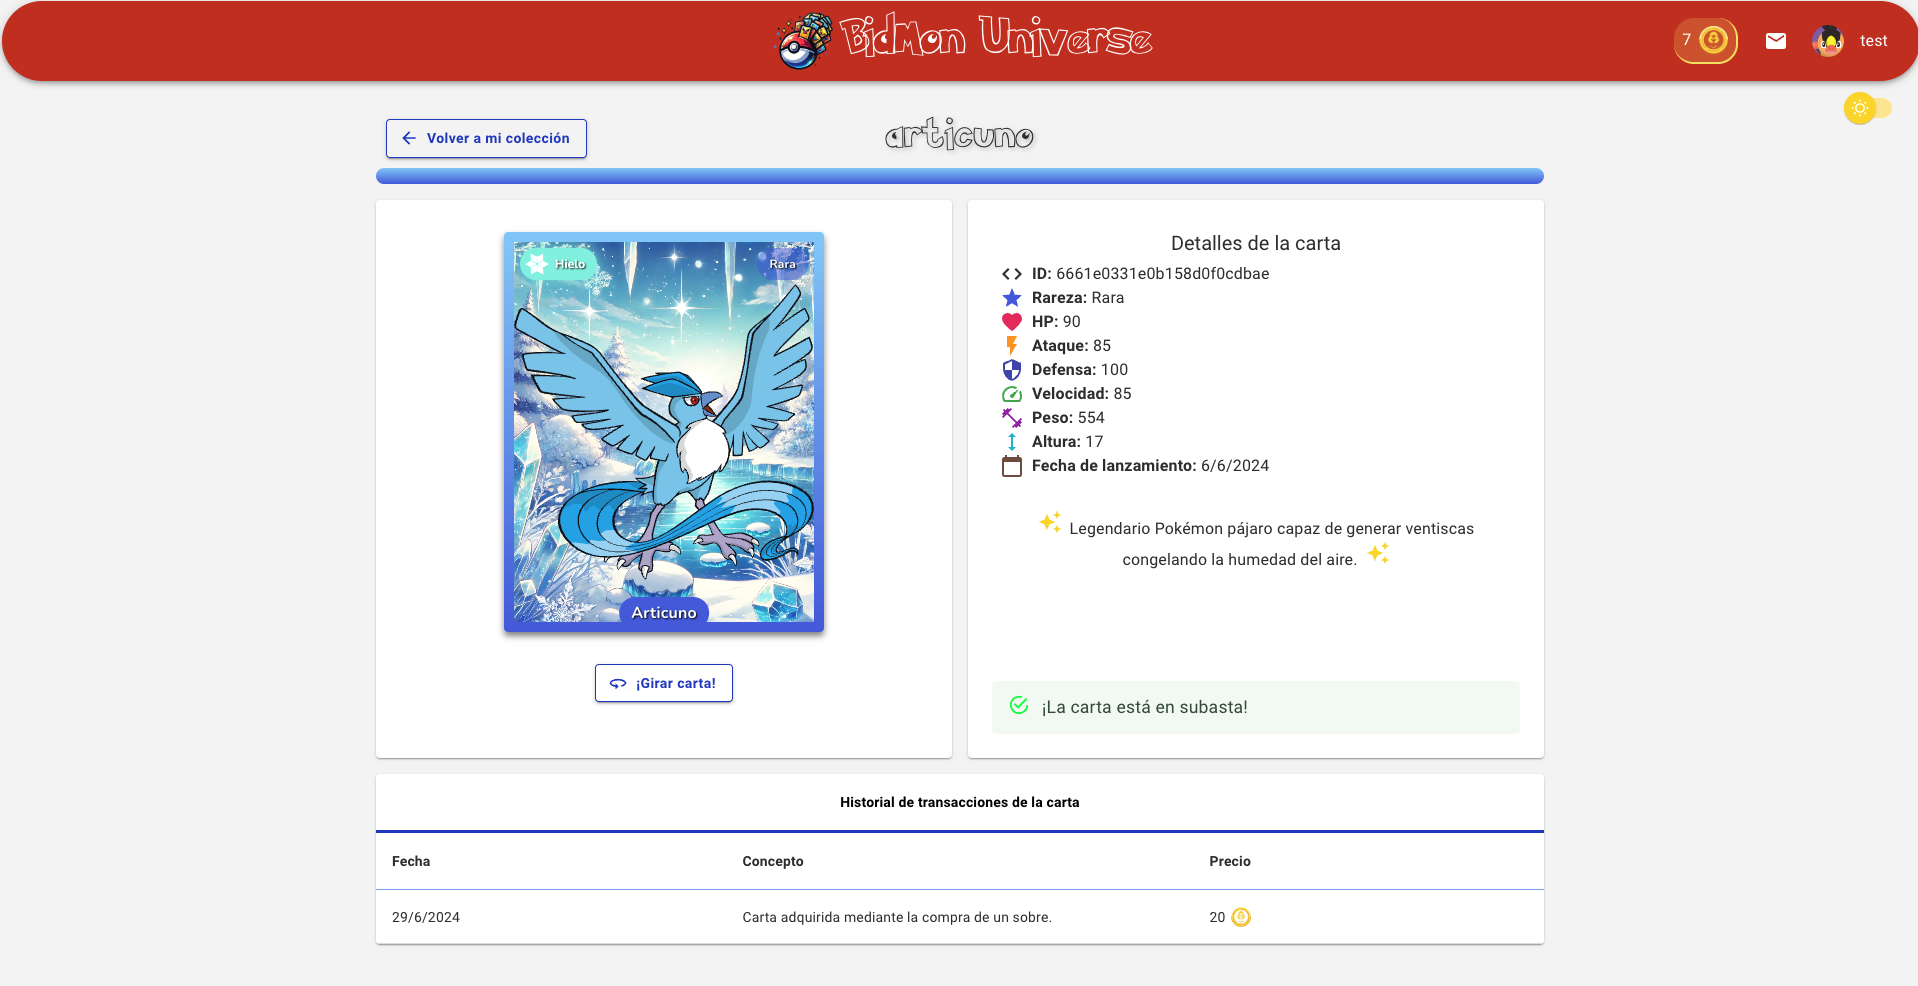
\includegraphics[width=0.8\textwidth]{figures/6-Analisis/6-Interfaz/interfaz/subasta_creada2.png}
    \caption{Alerta de que la carta está en subasta.}
    \label{fig:interfaz-subasta-alerta}
\end{figure}

Si el usuario cancelase en algún momento el proceso de subasta, se cerraría el modal.


\subsubsection{Compra de un sobre de cartas}
El proceso de compra de un sobre de cartas es más sencillo que el de la subasta de una carta.
El usuario pulsa el botón de \textit{Comprar sobre} del sobre que desea comprar y se le abrirá un modal de confirmación.

\begin{figure}[H]
    \centering
    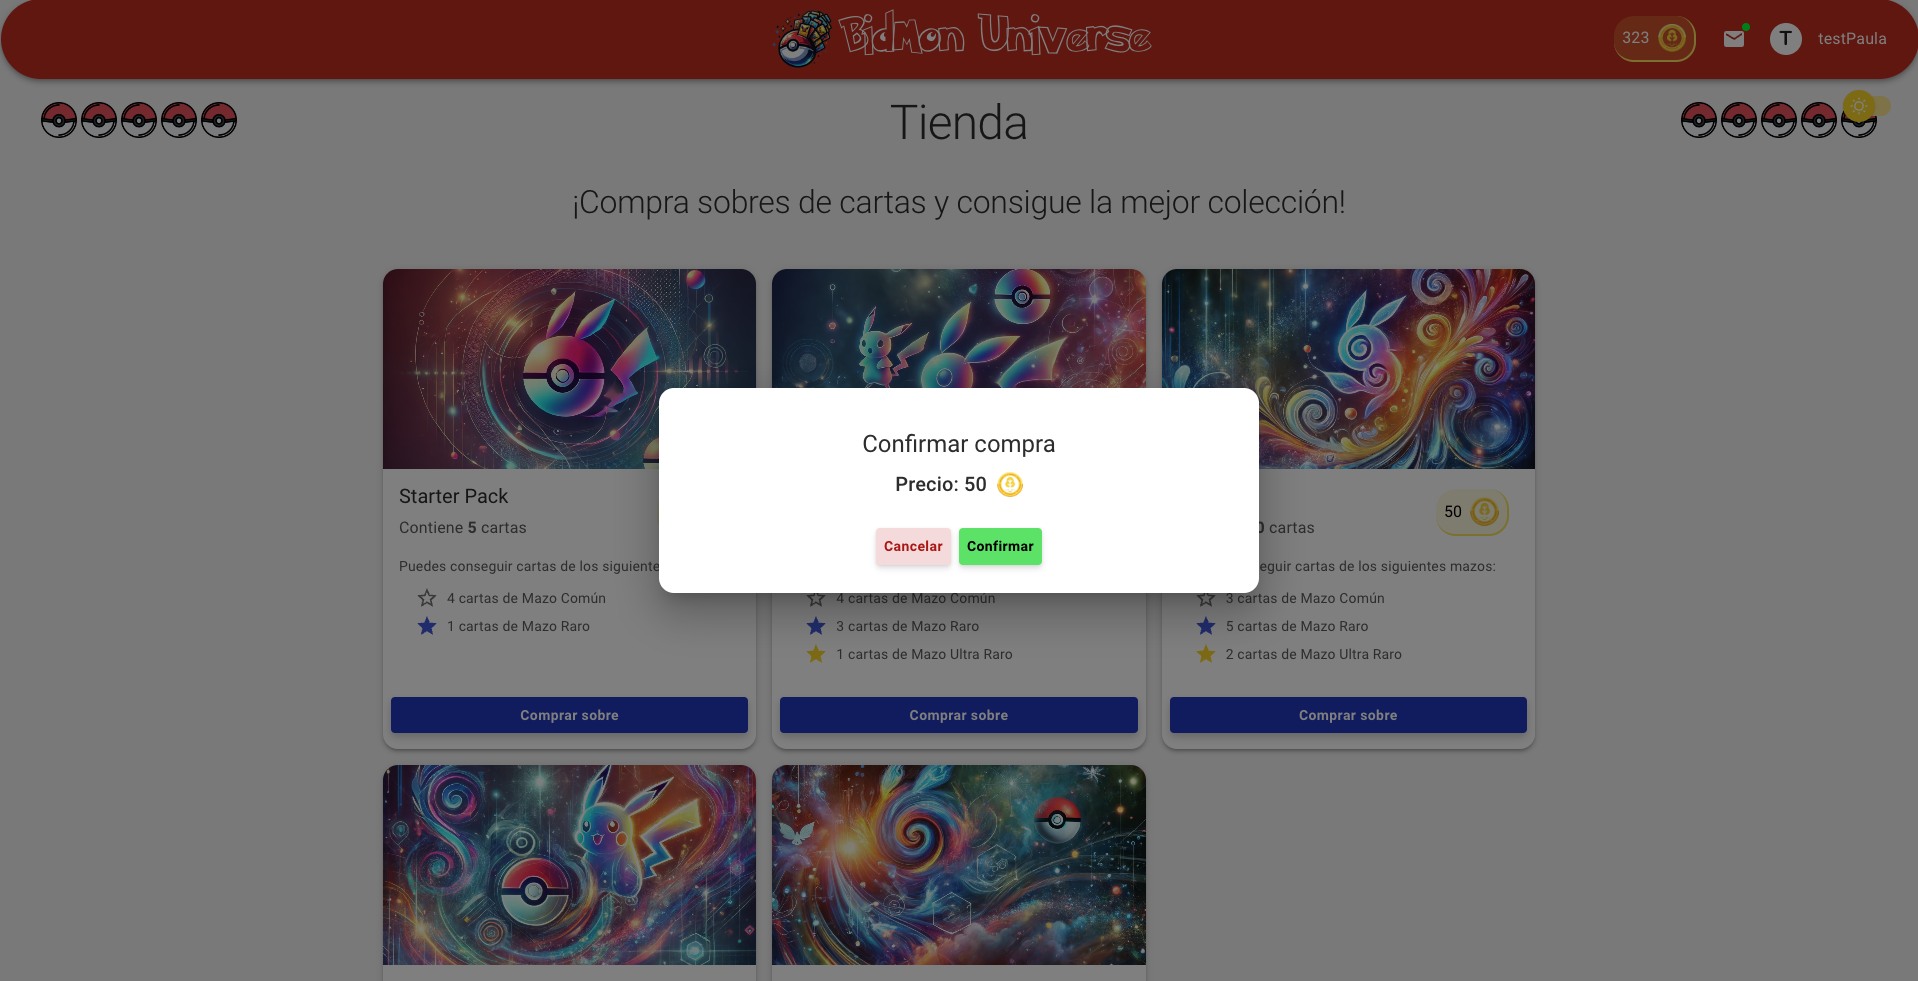
\includegraphics[width=0.8\textwidth]{figures/6-Analisis/6-Interfaz/interfaz/compra_sobre1.png}
    \caption{Modal de confirmación de compra de sobre.}
    \label{fig:interfaz-compra-sobre}
\end{figure}

Una vez que el usuario confirma la compra, se le mostrarán las cartas que ha obtenido en el sobre y un mensaje de éxito.
Estas cartas aparecen volteadas por lo que el usuario debe pulsar sobre ellas para verlas.
Tiene la opción de cerrar el modal o de ir a la colección de cartas para ver las cartas que ha obtenido.

\begin{figure}[H]
    \centering
    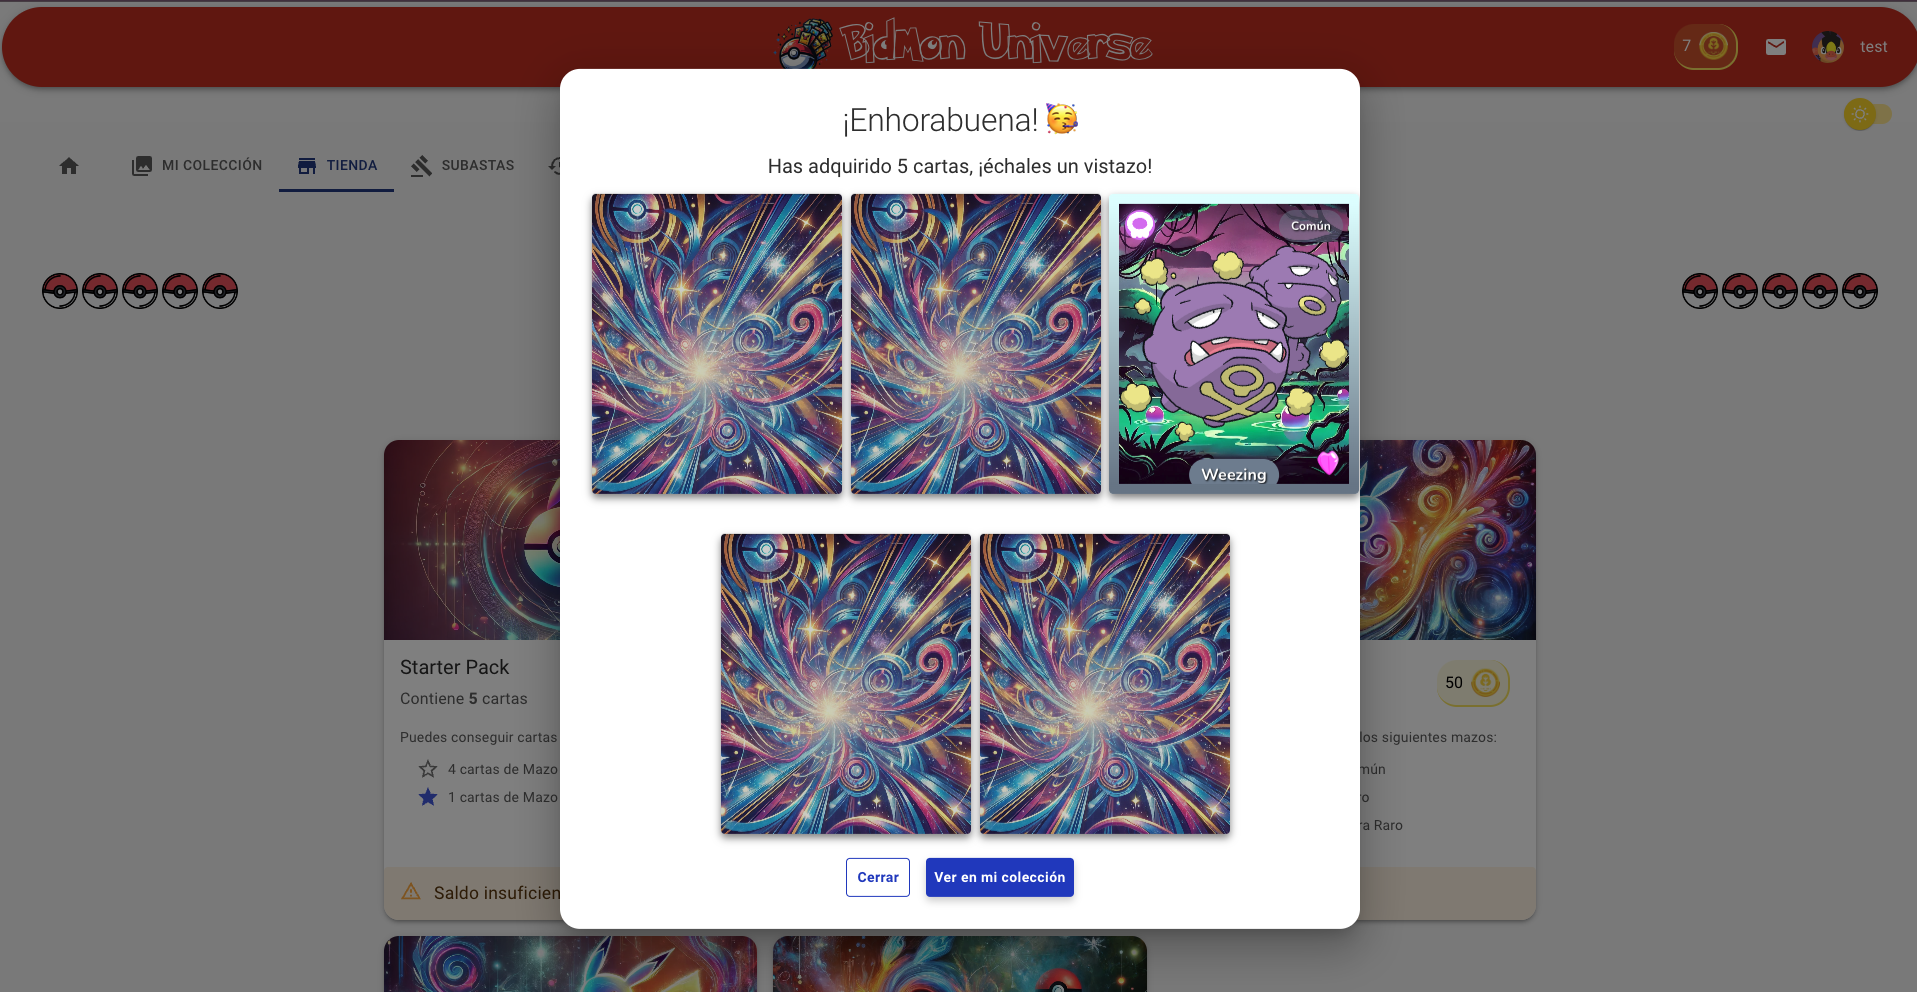
\includegraphics[width=0.8\textwidth]{figures/6-Analisis/6-Interfaz/interfaz/compra_sobre.png}
    \caption{Modal de cartas obtenidas en el sobre.}
    \label{fig:interfaz-sobre-comprado}
\end{figure}





\subsection{Diagrama de Navegabilidad}
En la sección \coloredUnderline{\hyperlink{sec:6_1-Identificacion_actores}{\ref*{sec:6_1-Identificacion_actores} \nameref*{sec:6_1-Identificacion_actores}}} se identificaron los actores del sistema,
cada uno con niveles de acceso y funcionalidades específicas adecuadas a su rol dentro de la plataforma. 

En este apartado se detalla el diagrama de navegabilidad de cada uno de los actores identificados en la sección mencionada anteriormente.
Para cada actor se detallan las vistas a las que puede acceder.

Las cajas que aparecen sombreadas en el diagrama representan las vistas que son accesibles desde cualquier otra vista,
debido a que se encuentran bien en el menú de navegación o en el pie de página de la aplicación.

La vista \textit{Home} es la vista principal de la aplicación, en función de si el usuario está autenticado o no, tendrá
una funcionalidad u otra, pero siempre es el punto de partida de la navegación y accesible desde cualquier vista.


\subsubsection{Usuario no autenticado}
En la \coloredUnderline{\hyperlink{fig:navegabilidad-usuario-no-autenticado}{Figura \ref*{fig:navegabilidad-usuario-no-autenticado}}} se muestra el diagrama de navegabilidad del usuario no autenticado.

\begin{figure}[H]
    \centering
    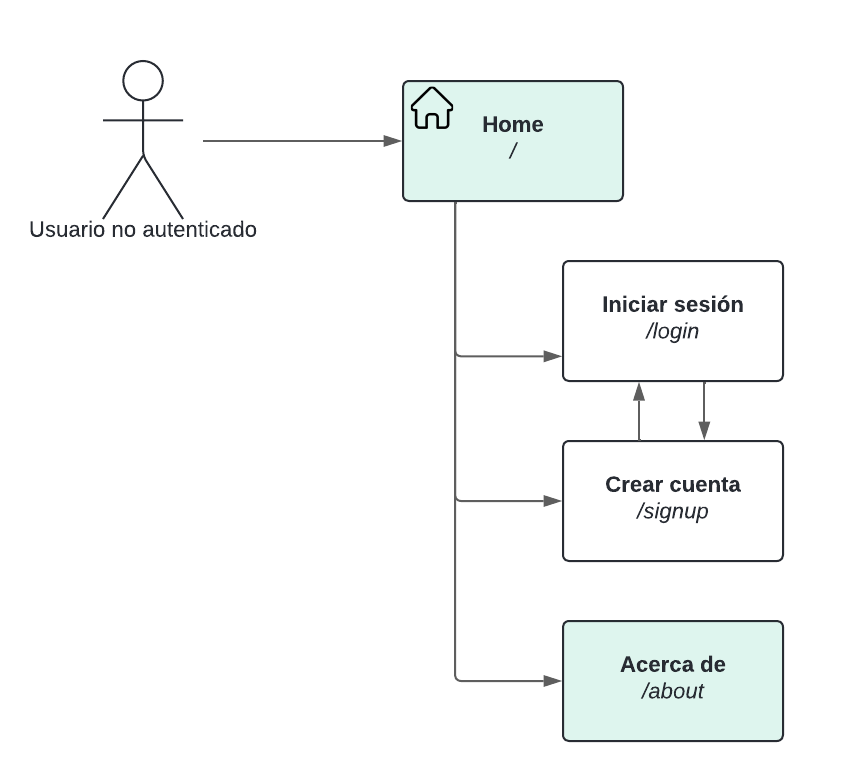
\includegraphics[width=0.5\textwidth]{figures/6-Analisis/6-Interfaz/navegabilidad-guest.png}
    \caption{Diagrama de navegabilidad del usuario no autenticado.}
    \hypertarget{fig:navegabilidad-usuario-no-autenticado}{}
    \label{fig:navegabilidad-usuario-no-autenticado}
\end{figure}

\subsubsection{Usuario autenticado}
En la \coloredUnderline{\hyperlink{fig:navegabilidad-usuario-autenticado}{Figura \ref*{fig:navegabilidad-usuario-autenticado}}} se muestra el diagrama de navegabilidad del usuario autenticado.

\begin{figure}[H]
    \centering
    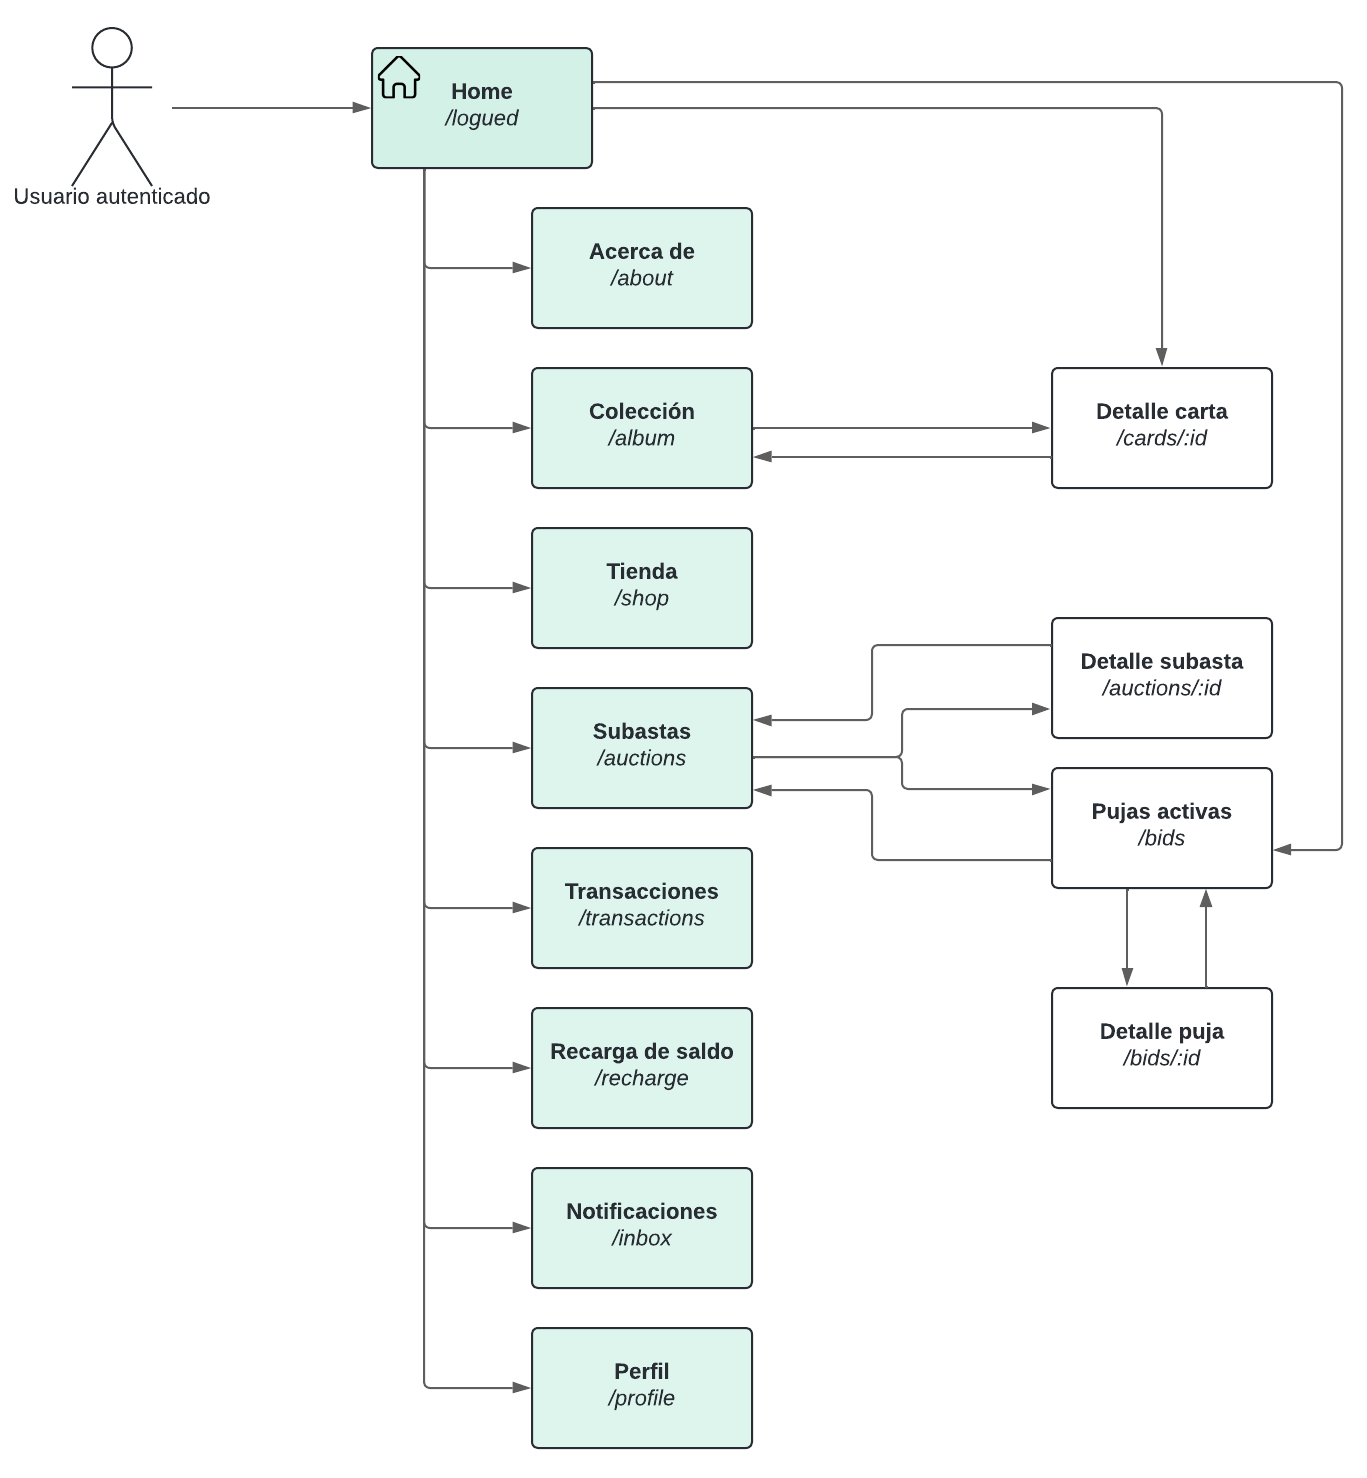
\includegraphics[width=0.8\textwidth]{figures/6-Analisis/6-Interfaz/navegabilidad-standard.png}
    \caption{Diagrama de navegabilidad del usuario autenticado.}
    \hypertarget{fig:navegabilidad-usuario-autenticado}{}
    \label{fig:navegabilidad-usuario-autenticado}
\end{figure}

\subsubsection{Administrador}
En la \coloredUnderline{\hyperlink{fig:navegabilidad-administrador}{Figura \ref*{fig:navegabilidad-administrador}}} se muestra el diagrama de navegabilidad del administrador.

\begin{figure}[H]
    \centering
    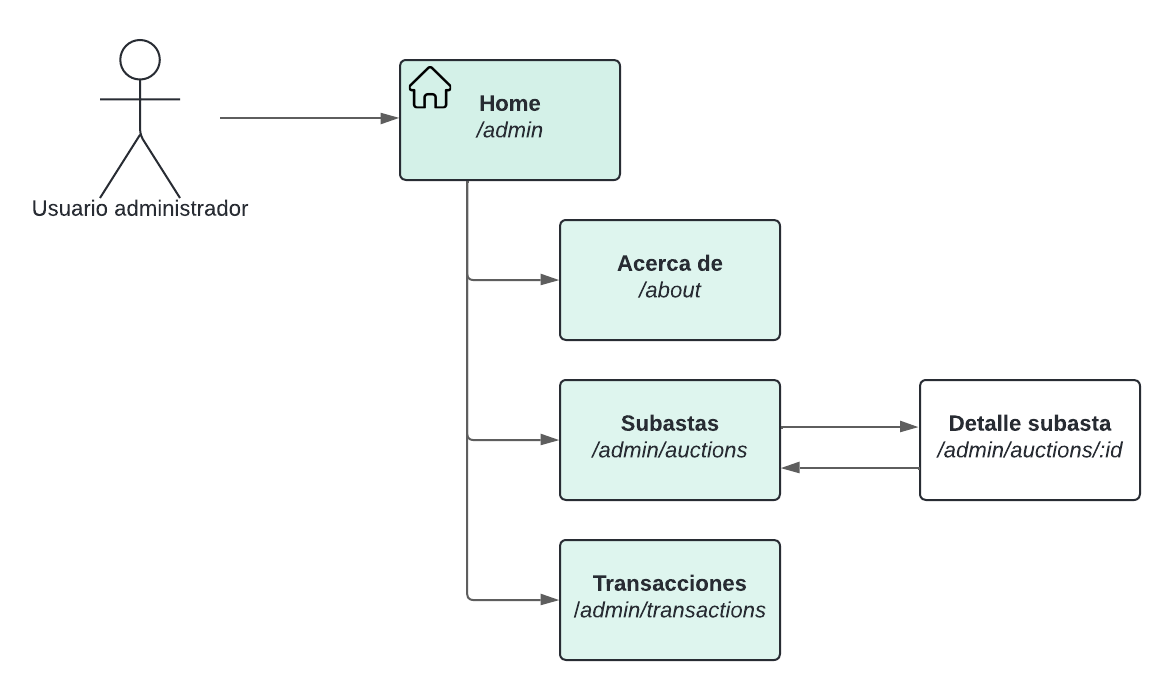
\includegraphics[width=0.6\textwidth]{figures/6-Analisis/6-Interfaz/navegabilidad-admin.png}
    \caption{Diagrama de navegabilidad del administrador.}
    \hypertarget{fig:navegabilidad-administrador}{}
    \label{fig:navegabilidad-administrador}
\end{figure}



\newpage
\section{ESPECIFICACIÓN DEL PLAN DE PRUEBAS}
% 6.8. Especificación del plan de pruebas + 7.6 Especificación Técnica del Plan de Pruebas
\subsection{Especificación del Plan de Pruebas}
Se realizarán cuatro tipos de pruebas para garantizar la calidad del sistema: pruebas unitarias, pruebas de integración, pruebas de usabilidad y pruebas de accesibilidad.
A continuación, se detallará cómo se llevarán a cabo las pruebas de cada tipo y se especificarán los criterios de aceptación para cada una de ellas.

\subsubsection{Pruebas Unitarias}
Las pruebas unitarias se realizarán para comprobar que cada componente del sistema funciona correctamente de forma aislada.
Se realizarán pruebas unitarias en el subsistema \textbf{restapi}, para comprobar que las rutas de la API REST funcionan correctamente, y en el subsistema \textbf{webapp}, para comprobar que los componentes de la interfaz de usuario se renderizan correctamente.

Para ello, se utilizará el framework de pruebas Jest para ambos subsistemas y se ejecutarán las pruebas en un entorno de test local.
Se espera que todas las pruebas unitarias pasen con éxito y que se alcance un porcentaje de cobertura de código mínima del 60\% para el subsistema \textbf{restapi} 
y para el subsistema \textbf{webapp} se deberán de cubrir los componentes que más se reutilizan en la aplicación.


Estas pruebas se realizarán en un entorno de test local, se utilizarán datos de prueba que simulan la información que se almacenará en la base de datos junto con una base de datos de pruebas.


\subsubsection{Pruebas de Integración}
Las pruebas de integración, también conocidas como pruebas de extremo a extremo o \textit{end-to-end}, se realizarán para comprobar que los distintos componentes del sistema funcionan correctamente en conjunto.
Se realizarán en el subsistema \textbf{webapp} con el framework de pruebas jest-cucumber y Puppeteer, que permite simular la interacción de un usuario con la aplicación y son muy descriptivas al iincluir escenarios de prueba escritos en lenguaje natural.
Estas pruebas se ejecutarán en un entorno de local de desarrollo y se utilizarán datos reales de la base de datos de desarrollo.

Los criterios de aceptación para estas pruebas son que se compruebe que un usuario puede iniciar sesión en la aplicación y que se renderice correctamente la página de inicio.

\subsubsection{Pruebas de Usabilidad}
Las pruebas de usabilidad se realizarán para comprobar que la interfaz de usuario es intuitiva y fácil de usar.
Se realizarán pruebas de usabilidad en el subsistema \textbf{webapp} con usuarios reales, que evaluarán la interfaz de usuario y proporcionarán retroalimentación sobre su usabilidad.
Estas pruebas se ejecutarán en un entorno de producción y se utilizarán datos reales de la base de datos de producción.
Los criterios de aceptación para estas pruebas son que no se reporten errores graves de usabilidad y que la interfaz de usuario sea fácil de usar para los usuarios reales.

\subsubsection{Pruebas de Accesibilidad}
Las pruebas de accesibilidad se realizarán para comprobar que la aplicación es accesible para personas con discapacidades.
Se utilizará el plugin de Google Chrome 
\coloredUnderline{\href{https://chromewebstore.google.com/detail/wave-evaluation-tool/jbbplnpkjmmeebjpijfedlgcdilocofh}{WAVE Evaluation Tool}} para comprobar la accesibilidad de la aplicación,
también se utilizará Google Lighthouse para comprobar la accesibilidad de la aplicación.

En un primer lugar se realizarán las pruebas de accesibilidad en el entorno de desarrollo y posteriormente, se repetirán en el entorno de producción con los errores corregidos.

Los criterios de aceptación para estas pruebas es que no haya errores de accesibilidad en el plugin WAVE Evaluation Tool,
permitiendo solo los errores de accesibilidad relacionados con el diseño específico de la aplicación.


\subsubsection{Pruebas de adaptabilidad}
Las pruebas de adaptabilidad se realizarán para comprobar que la aplicación se renderiza correctamente en distintos dispositivos y navegadores.
Las pruebas se realizarán en el entorno de producción y se utilizarán distintos dispositivos y navegadores para comprobar la adaptabilidad de la aplicación.
Los criterios de aceptación para estas pruebas son que la aplicación se renderice correctamente en dispositivos móviles, tabletas y ordenadores, y que funcione correctamente en los navegadores Google Chrome, Mozilla Firefox y Safari.


\subsection{Resultados de las Pruebas}
En esta sección se especificará en primer lugar las características del dispositivo y de los navegadores utilizados, y a continuación se detallarán los resultados de las pruebas realizadas.

\subsubsection{Dispositivo y navegadores utilizados}
Las pruebas se han llevado a cabo en un ordenador portátil con las siguientes características:
\begin{itemize}
    \item \textbf{Sistema Operativo}: macOS Sonoma 14.5.
    \item \textbf{Procesador}: Apple M3 Pro Max.
    \item \textbf{CPU}: 14 núcleos.
    \item \textbf{GPU}: 30 núcleos.
    \item \textbf{Memoria RAM}: 36 GB.
\end{itemize}

Como navegador se ha utilizado Google Chrome principalmente, las pruebas de adaptabilidad se han realizado además en Mozilla Firefox y Safari.
Las versiones de los navegadores son las siguientes:
\begin{itemize}
    \item \textbf{Google Chrome}: Versión 126.0.6478.127 (64 bits).
    \item \textbf{Mozilla Firefox}: Versión 127.0.2 (64 bits).
    \item \textbf{Safari}: Versión 17.5 (19618.2.12.11.6)
\end{itemize}


\subsubsection{Pruebas Unitarias}
Las pruebas unitarias se han realizado con éxito, se han comprobado que los componentes del sistema funcionan correctamente de forma aislada.
Se han realizado pruebas unitarias para cada \textit{router} del subsistema \textbf{restapi} y para los componentes más importantes del subsistema \textbf{webapp}. 

\subsubsubsection{Pruebas Unitarias. Restapi}
En el subsistema \textbf{restapi} se han realizado 51 pruebas unitarias, todas ellas han pasado con éxito obteniendo un 76.78\% de cobertura de código para \textit{routers}.
Se puede ver detallado el porcentaje de cobertura de código en la \coloredUnderline{\hyperlink{fig:6_8_Cobertura-Code-Restapi}{Figura \ref*{fig:6_8_Cobertura-Code-Restapi}: \nameref*{fig:6_8_Cobertura-Code-Restapi}}}.
\begin{figure}[H]
    \hypertarget{fig:6_8_Cobertura-Code-Restapi}{}
    \centering
    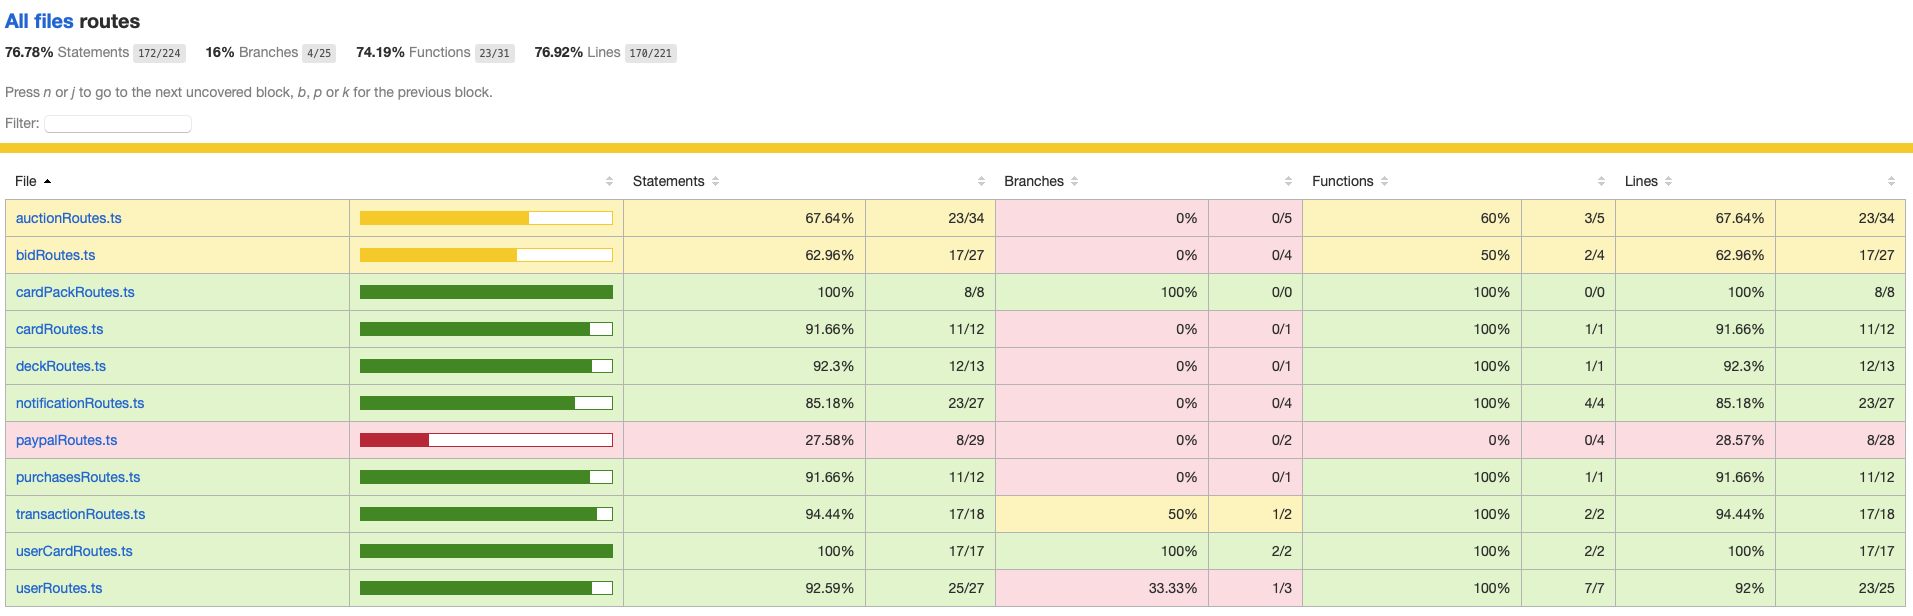
\includegraphics[width=0.8\linewidth]{figures/6-Analisis/6-Pruebas/6_8-Coverage-Restapi.png}
    \caption{Cobertura de Código del Subsistema restapi}
    \label{fig:6_8_Cobertura-Code-Restapi}
\end{figure}

A continuación, se detallan las pruebas unitarias realizadas en el subsistema \textbf{restapi}, con su descripición y resultado esperado.
Cabe destacar que para la ejecución de todas las pruebas, salvo para \textit{POST /api/users/login} y \textit{POST /api/users/signup}, se ha utilizado un token de autenticación válido, 
es decir, se ha iniciado sesión previamente con un usuario existente.


%-------------------TABLA PRUEBAS UNITARIAS RESTAPI-------------------

%-------------------TESTS DE AUCTIONROUTER-------------------
\begin{longtable}{
    >{\columncolor{lightgreen!20}}p{4cm}
    p{6cm}
    p{4cm}
    }
    \caption{Tests de auctionRouter} \label{table:test_auctionRouter} \\
    \toprule
    \rowcolor{darkgreen!50}
    \multicolumn{3}{|c|}{\textbf{Tests de auctionRouter}}\\
    \midrule
    \rowcolor{darkgreen!30}
    \textbf{Ruta a probar} & \multicolumn{1}{>{\columncolor{darkgreen!50}\centering\arraybackslash}p{6cm}}{\textbf{Descripción}} & \multicolumn{1}{>{\columncolor{darkgreen!50}\centering\arraybackslash}p{4cm}}{\textbf{Resultado esperado}} \\
    \endfirsthead
    
    \multicolumn{3}{c}%
    {{ \tablename\ \thetable{} Tests de auctionRouter -- continuación de la página anterior}} \\
    \toprule
    \rowcolor{darkgreen!50}
    \multicolumn{3}{|c|}{\textbf{Tests de auctionRouter}}\\
    \midrule
    \rowcolor{darkgreen!30}
    \textbf{Ruta a probar} & \multicolumn{1}{>{\columncolor{darkgreen!50}\centering\arraybackslash}p{6cm}}{\textbf{Descripción}} & \multicolumn{1}{>{\columncolor{darkgreen!50}\centering\arraybackslash}p{4cm}}{\textbf{Resultado esperado}} \\
    \midrule
    \endhead
    
    \midrule
    \multicolumn{3}{r}{{Continúa en la siguiente página...}} \\ 
    \endfoot
    
    \bottomrule
    \endlastfoot
    
    \midrule
    \textbf{GET /api/auctions} & Devuelve todas las subastas. & 200, la respuesta contiene una lista de subastas. \\
    \midrule
    \textbf{GET /api/auctions/a/:id} & Devuelve una subasta específica. & 200, la respuesta contiene los datos de la subasta. \\
    \midrule
    \textbf{GET /api/auctions/a/:id (no existe)} & Devuelve 404 si el ID de la subasta no se encuentra. & 404, la respuesta indica que la subasta no se encuentra. \\
    \midrule
    \textbf{GET /api/auctions/active/:username} & Devuelve todas las subastas activas para un nombre de usuario válido. & 200, la respuesta contiene una lista de subastas activas. \\
    \midrule
    \textbf{GET /api/auctions/active/u/:username} & Devuelve todas las subastas activas para un usuario. & 200, la respuesta contiene una lista de subastas activas. \\
    \end{longtable}

%-------------------TESTS DE BIDROUTER-------------------
\begin{longtable}{
    >{\columncolor{lightgreen!20}}p{4cm}
    p{6cm}
    p{4cm}
    }
    \caption{Tests de bidRouter} \label{table:test_bidRouter} \\
    \toprule
    \rowcolor{darkgreen!50}
    \multicolumn{3}{|c|}{\textbf{Tests de bidRouter}}\\
    \midrule
    \rowcolor{darkgreen!30}
    \textbf{Ruta a probar} & \multicolumn{1}{>{\columncolor{darkgreen!50}\centering\arraybackslash}p{6cm}}{\textbf{Descripción}} & \multicolumn{1}{>{\columncolor{darkgreen!50}\centering\arraybackslash}p{4cm}}{\textbf{Resultado esperado}} \\
    \endfirsthead
    
    \multicolumn{3}{c}%
    {{ \tablename\ \thetable{} Tests de bidRouter -- continuación de la página anterior}} \\
    \toprule
    \rowcolor{darkgreen!50}
    \multicolumn{3}{|c|}{\textbf{Tests de bidRouter}}\\
    \midrule
    \rowcolor{darkgreen!30}
    \textbf{Ruta a probar} & \multicolumn{1}{>{\columncolor{darkgreen!50}\centering\arraybackslash}p{6cm}}{\textbf{Descripción}} & \multicolumn{1}{>{\columncolor{darkgreen!50}\centering\arraybackslash}p{4cm}}{\textbf{Resultado esperado}} \\
    \midrule
    \endhead
    
    \midrule
    \multicolumn{3}{r}{{Continúa en la siguiente página...}} \\ 
    \endfoot
    
    \bottomrule
    \endlastfoot
    
    \midrule
    \textbf{GET /api/bids/b/:id} & Devuelve una oferta específica. & 200, la respuesta contiene los datos de la oferta. \\
    \midrule
    \textbf{GET /api/bids/b/:id (no existe)} & Devuelve 404 si el ID de la oferta no se encuentra. & 404, la respuesta indica que la oferta no se encuentra. \\
    \midrule
    \textbf{GET /api/bids/active/u/:username} & Devuelve todas las ofertas activas para un nombre de usuario válido. & 200, la respuesta contiene una lista de ofertas activas. \\
    \end{longtable}

%-------------------TESTS DE CARDPACKROUTER-------------------
\begin{longtable}{
    >{\columncolor{lightgreen!20}}p{4cm}
    p{6cm}
    p{4cm}
    }
    \caption{Tests de cardPackRouter} \label{table:test_cardPackRouter} \\
    \toprule
    \rowcolor{darkgreen!50}
    \multicolumn{3}{|c|}{\textbf{Tests de cardPackRouter}}\\
    \midrule
    \rowcolor{darkgreen!30}
    \textbf{Ruta a probar} & \multicolumn{1}{>{\columncolor{darkgreen!50}\centering\arraybackslash}p{6cm}}{\textbf{Descripción}} & \multicolumn{1}{>{\columncolor{darkgreen!50}\centering\arraybackslash}p{4cm}}{\textbf{Resultado esperado}} \\
    \endfirsthead
    
    \multicolumn{3}{c}%
    {{ \tablename\ \thetable{} Tests de cardPackRouter -- continuación de la página anterior}} \\
    \toprule
    \rowcolor{darkgreen!50}
    \multicolumn{3}{|c|}{\textbf{Tests de cardPackRouter}}\\
    \midrule
    \rowcolor{darkgreen!30}
    \textbf{Ruta a probar} & \multicolumn{1}{>{\columncolor{darkgreen!50}\centering\arraybackslash}p{6cm}}{\textbf{Descripción}} & \multicolumn{1}{>{\columncolor{darkgreen!50}\centering\arraybackslash}p{4cm}}{\textbf{Resultado esperado}} \\
    \midrule
    \endhead
    
    \midrule
    \multicolumn{3}{r}{{Continúa en la siguiente página...}} \\ 
    \endfoot
    
    \bottomrule
    \endlastfoot
    
    \midrule
    \textbf{GET /api/cardpacks} & Devuelve todos los paquetes de cartas disponibles. & 200, la respuesta contiene una lista de paquetes de cartas filtrados por disponibilidad. \\
    \end{longtable}

%-------------------TESTS DE CARDROUTER-------------------
\begin{longtable}{
    >{\columncolor{lightgreen!20}}p{4cm}
    p{6cm}
    p{4cm}
    }
    \caption{Tests de cardRouter} \label{table:test_cardRouter} \\
    \toprule
    \rowcolor{darkgreen!50}
    \multicolumn{3}{|c|}{\textbf{Tests de cardRouter}}\\
    \midrule
    \rowcolor{darkgreen!30}
    \textbf{Ruta a probar} & \multicolumn{1}{>{\columncolor{darkgreen!50}\centering\arraybackslash}p{6cm}}{\textbf{Descripción}} & \multicolumn{1}{>{\columncolor{darkgreen!50}\centering\arraybackslash}p{4cm}}{\textbf{Resultado esperado}} \\
    \endfirsthead
    
    \multicolumn{3}{c}%
    {{ \tablename\ \thetable{} Tests de cardRouter -- continuación de la página anterior}} \\
    \toprule
    \rowcolor{darkgreen!50}
    \multicolumn{3}{|c|}{\textbf{Tests de cardRouter}}\\
    \midrule
    \rowcolor{darkgreen!30}
    \textbf{Ruta a probar} & \multicolumn{1}{>{\columncolor{darkgreen!50}\centering\arraybackslash}p{6cm}}{\textbf{Descripción}} & \multicolumn{1}{>{\columncolor{darkgreen!50}\centering\arraybackslash}p{4cm}}{\textbf{Resultado esperado}} \\
    \midrule
    \endhead
    
    \midrule
    \multicolumn{3}{r}{{Continúa en la siguiente página...}} \\ 
    \endfoot
    
    \bottomrule
    \endlastfoot
    
    \midrule
    \textbf{GET /api/cards/:cardId} & Devuelve una carta por su ID. & 200, la respuesta contiene los datos de la carta, incluyendo el nombre 'bulbasaur'. \\
    \midrule
    \textbf{GET /api/cards/:cardId (no existe)} & Devuelve 404 si la carta no se encuentra. & 404, la respuesta contiene el mensaje 'Carta no encontrada.'. \\
    \midrule
    \textbf{GET /api/cards/:cardId (error)} & Maneja errores de forma adecuada. & 500, la respuesta contiene el mensaje 'Se ha producido un error al obtener la carta.'. \\
    \end{longtable}



%-------------------TESTS DE DECKROUTER-------------------

\begin{longtable}{
    >{\columncolor{lightgreen!20}}p{4cm}
    p{6cm}
    p{4cm}
    }
    \caption{Tests de deckRouter} \label{table:test_deckRouter} \\
    \toprule
    \rowcolor{darkgreen!50}
    \multicolumn{3}{|c|}{\textbf{Tests de deckRouter}}\\
    \midrule
    \rowcolor{darkgreen!30}
    \textbf{Ruta a probar} & \multicolumn{1}{>{\columncolor{darkgreen!50}\centering\arraybackslash}p{6cm}}{\textbf{Descripción}} & \multicolumn{1}{>{\columncolor{darkgreen!50}\centering\arraybackslash}p{4cm}}{\textbf{Resultado esperado}} \\
    \endfirsthead
    
    \multicolumn{3}{c}%
    {{ \tablename\ \thetable{} Tests de deckRouter -- continuación de la página anterior}} \\
    \toprule
    \rowcolor{darkgreen!50}
    \multicolumn{3}{|c|}{\textbf{Tests de deckRouter}}\\
    \midrule
    \rowcolor{darkgreen!30}
    \textbf{Ruta a probar} & \multicolumn{1}{>{\columncolor{darkgreen!50}\centering\arraybackslash}p{6cm}}{\textbf{Descripción}} & \multicolumn{1}{>{\columncolor{darkgreen!50}\centering\arraybackslash}p{4cm}}{\textbf{Resultado esperado}} \\
    \midrule
    \endhead
    
    \midrule
    \multicolumn{3}{r}{{Continúa en la siguiente página...}} \\ 
    \endfoot
    
    \bottomrule
    \endlastfoot
    
    \midrule
    \textbf{GET /api/decks} & Devuelve todos los mazos de cartas. & 200, la respuesta contiene una lista de mazos de cartas. \\
    \midrule
    \textbf{GET /api/decks/:deckid} & Devuelve un mazo de cartas por su ID. & 200, la respuesta contiene los datos del mazo de cartas, incluyendo 'deckId', 'name', 'type', y 'publicationDate'. \\
    \midrule
    \textbf{GET /api/decks (error)} & Maneja errores de forma adecuada al obtener todos los mazos de cartas. & 500, la respuesta contiene el mensaje 'Se ha producido un error al obtener los mazos de cartas.'. \\
    \midrule
    \textbf{GET /api/decks/:deckid (no existe)} & Devuelve 404 si el mazo de cartas no se encuentra. & 404, la respuesta contiene el mensaje 'Mazo de cartas no encontrado.'. \\
    \midrule
    \textbf{GET /api/decks/:deckid (error)} & Maneja errores de forma adecuada al obtener un mazo de cartas por su ID. & 500, la respuesta contiene el mensaje 'Se ha producido un error al obtener el mazo de cartas.'. \\
    \end{longtable}


%-------------------TESTS DE NOTIFICATIONROUTER-------------------
\begin{longtable}{
    >{\columncolor{lightgreen!20}}p{4cm}
    p{6cm}
    p{4cm}
    }
    \caption{Tests de notificationRouter} \label{table:test_notificationRouter} \\
    \toprule
    \rowcolor{darkgreen!50}
    \multicolumn{3}{|c|}{\textbf{Tests de notificationRouter}}\\
    \midrule
    \rowcolor{darkgreen!30}
    \textbf{Ruta a probar} & \multicolumn{1}{>{\columncolor{darkgreen!50}\centering\arraybackslash}p{6cm}}{\textbf{Descripción}} & \multicolumn{1}{>{\columncolor{darkgreen!50}\centering\arraybackslash}p{4cm}}{\textbf{Resultado esperado}} \\
    \endfirsthead
    
    \multicolumn{3}{c}%
    {{ \tablename\ \thetable{} Tests de notificationRouter -- continuación de la página anterior}} \\
    \toprule
    \rowcolor{darkgreen!50}
    \multicolumn{3}{|c|}{\textbf{Tests de notificationRouter}}\\
    \midrule
    \rowcolor{darkgreen!30}
    \textbf{Ruta a probar} & \multicolumn{1}{>{\columncolor{darkgreen!50}\centering\arraybackslash}p{6cm}}{\textbf{Descripción}} & \multicolumn{1}{>{\columncolor{darkgreen!50}\centering\arraybackslash}p{4cm}}{\textbf{Resultado esperado}} \\
    \midrule
    \endhead
    
    \midrule
    \multicolumn{3}{r}{{Continúa en la siguiente página...}} \\ 
    \endfoot
    
    \bottomrule
    \endlastfoot
    
    \midrule
    \textbf{GET /api/notifications/:username} & Devuelve todas las notificaciones para un nombre de usuario válido. & 200, la respuesta contiene una lista de notificaciones. \\
    \midrule
    \textbf{GET /api/notifications/unread/:username} & Devuelve todas las notificaciones no leídas para un nombre de usuario válido. & 200, la respuesta contiene una lista de notificaciones no leídas. \\
    \midrule
    \textbf{PATCH /api/notifications/notification/:notificationId/read} & Marca una notificación como leída. & 200, la respuesta indica éxito. \\
    \midrule
    \textbf{PATCH /api/notifications/read/:username} & Marca todas las notificaciones de un usuario como leídas. & 200, la respuesta indica éxito. \\
    \end{longtable}


%-------------------TESTS DE PURCHASESROUTER-------------------
\begin{longtable}{
    >{\columncolor{lightgreen!20}}p{4cm}
    p{6cm}
    p{4cm}
    }
    \caption{Tests de purchasesRouter} \label{table:test_purchasesRouter} \\
    \toprule
    \rowcolor{darkgreen!50}
    \multicolumn{3}{|c|}{\textbf{Tests de purchasesRouter}}\\
    \midrule
    \rowcolor{darkgreen!30}
    \textbf{Ruta a probar} & \multicolumn{1}{>{\columncolor{darkgreen!50}\centering\arraybackslash}p{6cm}}{\textbf{Descripción}} & \multicolumn{1}{>{\columncolor{darkgreen!50}\centering\arraybackslash}p{4cm}}{\textbf{Resultado esperado}} \\
    \endfirsthead
    
    \multicolumn{3}{c}%
    {{ \tablename\ \thetable{} Tests de purchasesRouter -- continuación de la página anterior}} \\
    \toprule
    \rowcolor{darkgreen!50}
    \multicolumn{3}{|c|}{\textbf{Tests de purchasesRouter}}\\
    \midrule
    \rowcolor{darkgreen!30}
    \textbf{Ruta a probar} & \multicolumn{1}{>{\columncolor{darkgreen!50}\centering\arraybackslash}p{6cm}}{\textbf{Descripción}} & \multicolumn{1}{>{\columncolor{darkgreen!50}\centering\arraybackslash}p{4cm}}{\textbf{Resultado esperado}} \\
    \midrule
    \endhead
    
    \midrule
    \multicolumn{3}{r}{{Continúa en la siguiente página...}} \\ 
    \endfoot
    
    \bottomrule
    \endlastfoot
    
    \midrule
    \textbf{POST /api/purchases/cardpack} & Compra un paquete de cartas exitosamente, disminuyendo la cantidad disponible del paquete y el saldo del usuario, creando cartas de usuario y transacciones. & 200, la respuesta indica éxito y las verificaciones post-compra son correctas. \\
    \midrule
    \textbf{POST /api/purchases/cardpack (usuario no existe)} & Maneja errores cuando el usuario no existe. & 500, la respuesta contiene el mensaje 'El usuario no existe.'. \\
    \midrule
    \textbf{POST /api/purchases/cardpack (saldo insuficiente)} & Maneja errores cuando el usuario no tiene suficiente saldo. & 500, la respuesta indica un error de saldo insuficiente. \\
    \midrule
    \textbf{POST /api/purchases/cardpack (paquete no existe)} & Maneja errores cuando el paquete de cartas no existe. & 500, la respuesta indica que el paquete de cartas no se encuentra. \\
    \midrule
    \textbf{POST /api/purchases/cardpack (paquete no disponible)} & Maneja errores cuando el paquete de cartas no está disponible. & 500, la respuesta indica que el paquete de cartas no está disponible. \\
    \end{longtable}



%-------------------TESTS DE TRANSACTIONROUTER-------------------
\begin{longtable}{
    >{\columncolor{lightgreen!20}}p{4cm}
    p{6cm}
    p{4cm}
    }
    \caption{Tests de transactionRouter} \label{table:descripcion_transactionRouter} \\
    \toprule
    \rowcolor{darkgreen!50}
    \multicolumn{3}{|c|}{\textbf{Tests de transactionRouter}}\\
    \midrule
    \rowcolor{darkgreen!30}
    \textbf{Ruta a probar} & \multicolumn{1}{>{\columncolor{darkgreen!50}\centering\arraybackslash}p{6cm}}{\textbf{Descripción}} & \multicolumn{1}{>{\columncolor{darkgreen!50}\centering\arraybackslash}p{4cm}}{\textbf{Resultado esperado}} \\
    \endfirsthead
    
    \multicolumn{3}{c}%
    {{ \tablename\ \thetable{} Tests de transactionRouter -- continuación de la página anterior}} \\
    \toprule
    \rowcolor{darkgreen!50}
    \multicolumn{3}{|c|}{\textbf{Tests de transactionRouter}}\\
    \midrule
    \rowcolor{darkgreen!30}
    \textbf{Ruta a probar} & \multicolumn{1}{>{\columncolor{darkgreen!50}\centering\arraybackslash}p{6cm}}{\textbf{Descripción}} & \multicolumn{1}{>{\columncolor{darkgreen!50}\centering\arraybackslash}p{4cm}}{\textbf{Resultado esperado}} \\
    \midrule
    \endhead
    
    \midrule
    \multicolumn{3}{r}{{Continúa en la siguiente página...}} \\ 
    \endfoot
    
    \bottomrule
    \endlastfoot
    
    \midrule
    \textbf{GET /api/transactions} & Devuelve todas las transacciones. & 200, la respuesta contiene una lista de transacciones. \\
    \midrule
    \textbf{GET /api/transactions/u/:username} & Devuelve las transacciones para un nombre de usuario válido. & 200, la respuesta contiene una lista de transacciones para el usuario. \\
    \midrule
    \textbf{GET /api/transactions/c/:userCardId} & Devuelve las transacciones para un ID de carta de usuario válido. & 200, la respuesta contiene una lista de transacciones para la carta de usuario. \\
    \midrule
    \textbf{GET /api/transactions (no admin)} & Devuelve 403 si el usuario no es administrador. & 403, la respuesta contiene el mensaje 'Acceso denegado. Se requiere rol de administrador.'. \\
    \midrule
    \textbf{GET /api/transactions/u/:username (username inválido)} & Devuelve 400 para un nombre de usuario inválido. & 400, la respuesta contiene errores de validación para el nombre de usuario. \\
    \end{longtable}



%-------------------TESTS DE USERCARDROUTER-------------------
\begin{longtable}{
    >{\columncolor{lightgreen!20}}p{4cm}
    p{6cm}
    p{4cm}
    }
    \caption{Tests de userCardRouter} \label{table:test_userCardRouter} \\
    \toprule
    \rowcolor{darkgreen!50}
    \multicolumn{3}{|c|}{\textbf{Tests de userCardRouter}}\\
    \midrule
    \rowcolor{darkgreen!30}
    \textbf{Ruta a probar} & \multicolumn{1}{>{\columncolor{darkgreen!50}\centering\arraybackslash}p{6cm}}{\textbf{Descripción}} & \multicolumn{1}{>{\columncolor{darkgreen!50}\centering\arraybackslash}p{4cm}}{\textbf{Resultado esperado}} \\
    \endfirsthead
    
    \multicolumn{3}{c}%
    {{ \tablename\ \thetable{} Tests de userCardRouter -- continuación de la página anterior}} \\
    \toprule
    \rowcolor{darkgreen!50}
    \multicolumn{3}{|c|}{\textbf{Tests de userCardRouter}}\\
    \midrule
    \rowcolor{darkgreen!30}
    \textbf{Ruta a probar} & \multicolumn{1}{>{\columncolor{darkgreen!50}\centering\arraybackslash}p{6cm}}{\textbf{Descripción}} & \multicolumn{1}{>{\columncolor{darkgreen!50}\centering\arraybackslash}p{4cm}}{\textbf{Resultado esperado}} \\
    \midrule
    \endhead
    
    \midrule
    \multicolumn{3}{r}{{Continúa en la siguiente página...}} \\ 
    \endfoot
    
    \bottomrule
    \endlastfoot
    
    \midrule
    \textbf{GET /api/usercards/u/:username} & Devuelve las tarjetas de usuario para un nombre de usuario válido. & 200, la respuesta contiene un arreglo de tarjetas de usuario. \\
    \midrule
    \textbf{GET /api/usercards/:id} & Devuelve una tarjeta de usuario específica. & 200, la respuesta contiene la tarjeta de usuario con el campo 'legibleCardId'. \\
    \midrule
    \textbf{GET /api/usercards/:id (no existe)} & Devuelve 404 si la tarjeta de usuario no se encuentra. & 404, la respuesta indica que la tarjeta de usuario no se encuentra. \\
    \midrule
    \textbf{GET /api/usercards/:id (ID inválido)} & Devuelve 400 para un ID de tarjeta de usuario inválido. & 400, la respuesta indica un error. \\
    \midrule
    \textbf{GET /api/usercards/u/:username (nombre de usuario muy largo)} & Devuelve 400 si el nombre de usuario es demasiado largo. & 400, la respuesta indica un error con un mensaje sobre la longitud del nombre de usuario. \\
    \end{longtable}

%-------------------TESTS DE USERROUTER-------------------
\begin{longtable}{
    >{\columncolor{lightgreen!20}}p{4cm}
    p{6cm}
    p{4cm}
    }
    \caption{Tests de userRouter} \label{table:test_userRouter} \\
    \toprule
    \rowcolor{darkgreen!50}
    \multicolumn{3}{|c|}{\textbf{Tests de userRouter}}\\
    \midrule
    \rowcolor{darkgreen!30}
    \textbf{Ruta a probar} & \multicolumn{1}{>{\columncolor{darkgreen!50}\centering\arraybackslash}p{6cm}}{\textbf{Descripción}} & \multicolumn{1}{>{\columncolor{darkgreen!50}\centering\arraybackslash}p{4cm}}{\textbf{Resultado esperado}} \\
    \endfirsthead
    
    \multicolumn{3}{c}%
    {{ \tablename\ \thetable{} Tests de userRouter -- continuación de la página anterior}} \\
    \toprule
    \rowcolor{darkgreen!50}
    \multicolumn{3}{|c|}{\textbf{Tests de userRouter}}\\
    \midrule
    \rowcolor{darkgreen!30}
    \textbf{Ruta a probar} & \multicolumn{1}{>{\columncolor{darkgreen!50}\centering\arraybackslash}p{6cm}}{\textbf{Descripción}} & \multicolumn{1}{>{\columncolor{darkgreen!50}\centering\arraybackslash}p{4cm}}{\textbf{Resultado esperado}} \\
    \midrule
    \endhead
    
    \midrule
    \multicolumn{3}{r}{{Continúa en la siguiente página...}} \\ 
    \endfoot
    
    \bottomrule
    \endlastfoot
    
    \midrule
    \textbf{POST /api/users/login} & Inicia sesión un usuario existente con el nombre de usuario 'test' y la contraseña 'Password123-'. & 200, la respuesta contiene un token y datos del usuario. \\
    \midrule
    \textbf{POST /api/users/signup} & Crea un nuevo usuario con el nombre de usuario 'newuser' y la contraseña 'Password123-'. & 201, la respuesta contiene un mensaje de éxito y datos del nuevo usuario. \\
    \midrule
    \textbf{GET /api/users/:username} & Obtiene los detalles del usuario 'test' con un token válido. & 200, la respuesta contiene los datos del usuario. \\
    \midrule
    \textbf{PATCH /api/users/update/avatar} & Actualiza la imagen de perfil del usuario 'test' a 'avatar1.png'. & 200, la respuesta indica éxito. \\
    \midrule
    \textbf{PATCH /api/users/update/pass} & Actualiza la contraseña del usuario 'test' a 'NewPass1234-'. & 200, la respuesta indica éxito. \\
    \midrule
    \textbf{GET /api/users/:username (error handling)} & Devuelve 400 si el nombre de usuario es demasiado largo. & 400, la respuesta indica error. \\
    \midrule
    \textbf{GET /api/users/:username (sin token)} & Devuelve 401 si no se proporciona un token. & 401, la respuesta indica error. \\
    \midrule
    \textbf{GET /api/users/:username (usuario no encontrado)} & Devuelve 404 si el usuario no se encuentra. & 404, la respuesta contiene mensaje de usuario no encontrado. \\
    \midrule
    \textbf{GET /api/users/:username (error)} & Maneja errores de forma adecuada. & 500, la respuesta indica error interno. \\
    \midrule
    \textbf{POST /api/users/login (usuario no existe)} & Devuelve 401 si el usuario no existe. & 401, la respuesta indica error. \\
    \midrule
    \textbf{POST /api/users/login (contraseña incorrecta)} & Devuelve 401 si la contraseña es incorrecta. & 401, la respuesta indica error. \\
    \midrule
    \textbf{POST /api/users/login (error)} & Maneja errores de forma adecuada. & 500, la respuesta indica error interno. \\
    \midrule
    \textbf{POST /api/users/signup (usuario ya existe)} & Devuelve 400 si el nombre de usuario ya existe. & 400, la respuesta indica error. \\
    \midrule
    \textbf{POST /api/users/signup (datos incompletos)} & Devuelve 400 si falta el nombre de usuario, contraseña o fecha de nacimiento. & 400, la respuesta indica error. \\
    \midrule
    \textbf{POST /api/users/signup (error)} & Maneja errores de forma adecuada. & 500, la respuesta contiene mensaje de error y autenticación fallida. \\
    \end{longtable}




\subsubsubsection{Pruebas Unitarias. Webapp}
En el subsistema \textbf{webapp} se han realizado 9 pruebas unitarias automáticas, se han probado los componentes más importantes de la aplicación y todas han pasado con éxito.
El resto de componentes se han probado de forma manual y se ha comprobado que su comportamiento es el esperado.
Las pruebas unitarias automáticas se han realizado sobre los componentes que más se reutilizan en la aplicación, estos son:
\begin{itemize}
    \item \textbf{Componente \textit{Button}}: Se ha comprobado que el componente \textit{Button} renderiza correctamente, que se muestra el texto esperado y que se ejecuta la función \textit{onClick} cuando se hace clic en el botón.
    \item \textbf{Componente \textit{Calendar}}: Se ha comprobado que el componente \textit{Calendar} renderiza correctamente, que se ejecuta la función \textit{onChange} cuando se selecciona una fecha y que si hay un error en la fecha se muestre un mensaje de error.
    \item \textbf{Componente \textit{ErrorMessageBox}}: Se ha comprobado que el componente \textit{ErrorMessageBox} renderiza correctamente y que redirige a la página de inicio cuando se hace clic en el botón que contiene.
    \item \textbf{Componente \textit{PokemonCard}}: Se ha comprobado que la carta de Pokémon se renderiza correctamente y que se ejecutan los distintos \textit{onClick} dependiendo de su configuración inicial.
\end{itemize}
En la figura \coloredUnderline{\hyperlink{fig:coverage_webapp}{Figura \ref*{fig:coverage_webapp}. \nameref*{fig:coverage_webapp}}} se muestran los resultados de las pruebas unitarias automáticas realizadas.
\begin{figure}[H]
    \centering
    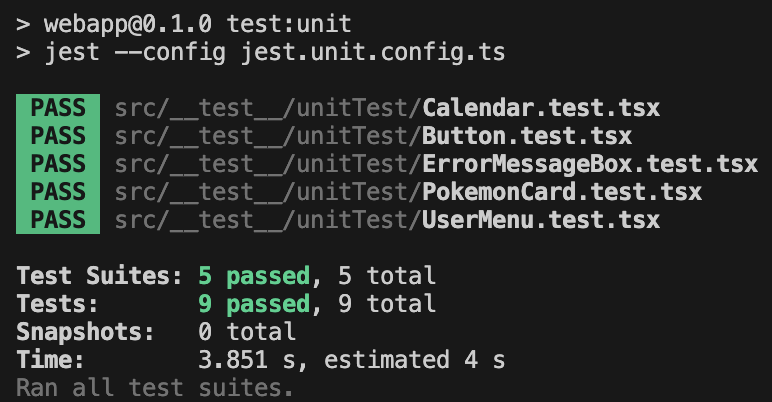
\includegraphics[width=0.5\textwidth]{figures/6-Analisis/6-Pruebas/6_8_webapp-unit.png}
    \caption{Resultados de las pruebas unitarias automáticas de la webapp}
    \hypertarget{fig:coverage_webapp}{}
    \label{fig:coverage_webapp}
\end{figure}

\subsubsection{Pruebas de Integración}
Las pruebas de integración se han realizado con éxito, se han comprobado que los distintos componentes del sistema funcionan correctamente en conjunto.
Se han realizado pruebas de integración en el subsistema \textbf{webapp} con el framework jest-cucumber y Puppeteer.
Se han realizado 3 pruebas de integración automáticas, todas ellas han pasado con éxito.
Las pruebas que se han realizado son las siguientes:
\begin{itemize}
    \item \textbf{Prueba de Inicio de Sesión Exitoso}: Se ha comprobado que el inicio de sesión funciona correctamente. De esta forma, se ha comprobado que el usuario puede iniciar sesión con sus credenciales y acceder a la aplicación, 
    lo que significa que la conexión con el backend funciona correctamente y la integración de los componentes de la aplicación es correcta.
    \item \textbf{Prueba de Inicio de Sesión Fallido}: Se ha comprobado que el inicio de sesión falla cuando las credenciales son incorrectas. De esta forma, se ha comprobado que la aplicación responde correctamente a errores en el inicio de sesión.
     \item \textbf{Prueba de Registro de Usuario Fallido}: Se ha comprobado que el registro de usuario falla cuando los datos introducidos no son válidos. 
     Se verifica que la aplicación responde correctamente a errores en el registro de usuario y se resaltan los campos con errores.
\end{itemize}

En la figura \coloredUnderline{\hyperlink{fig:coverage_webapp2}{Figura \ref*{fig:coverage_webapp}. \nameref*{fig:coverage_webapp}}} se muestran los resultados de las pruebas de integración automáticas realizadas.
\begin{figure}[H]
    \centering
    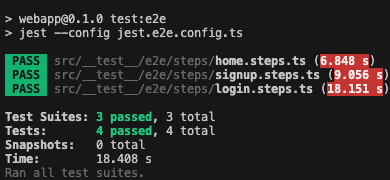
\includegraphics[width=0.5\textwidth]{figures/6-Analisis/6-Pruebas/6_8_webapp-e2e.png}
    \caption{Resultados de las pruebas de integración automáticas de la webapp}
    \hypertarget{fig:coverage_webapp2}{}
    \label{fig:coverage_webapp2}
\end{figure}

El resto de pruebas de integración se han realizado de forma manual y se ha comprobado que el comportamiento de la aplicación es el esperado.

\subsubsection{Pruebas de Usabilidad}
Se ha creado un formulario de evaluación de usabilidad que se les ha proporcionado a los usuarios para que evalúen la interfaz de usuario.
Se han realizado pruebas de usabilidad con 3 usuarios reales, que han evaluado la interfaz de usuario y han proporcionado retroalimentación sobre su usabilidad.
Estos usuarios, que no han participado en el desarrollo de la aplicación, han tenido que completar una serie de tareas y responder a preguntas sobre la usabilidad de la aplicación.
Los usuarios tienen una experiencia variada en el uso de aplicaciones web y representan a los diferentes tipos de usuarios que utilizarán la aplicación.
Los datos de los usuarios son los siguientes:
\begin{itemize}
    \item \textbf{Usuario 1}: Hombre de 51 años, con poca experiencia en el uso de aplicaciones web. No ha utilizado aplicaciones similares anteriormente ni realizado compras en línea.
    \item \textbf{Usuario 2}: Mujer de 22 años, con mucha experiencia en el uso de aplicaciones web. Ha utilizado aplicaciones similares anteriormente y ha realizado compras en línea.
    \item \textbf{Usuario 3}: Mujer de 18 años, con experiencia en el uso de aplicaciones web. Ha utilizado aplicaciones similares anteriormente, pero no ha llegado a realizar compras en ellas.
\end{itemize}

\subsubsubsection{Cuestionario de usabilidad}
Se ha realizado un cuestionario de usabilidad con distintas preguntas para evaluar la calidad de la interfaz de usuario de la aplicación.
Estas preguntas pretenden evaluar la calidad del diseño de la interfaz, la facilidad de uso y la satisfacción del usuario.
Este cuestionario se ha proporcionado a los usuarios para que lo completen después de realizar las tareas asignadas.
En la tabla  \coloredUnderline{\hyperlink{table:cuestionario_usabilidad}{Tabla \ref*{table:cuestionario_usabilidad}. \nameref*{table:cuestionario_usabilidad}}} se muestra el cuestionario de usabilidad que se ha proporcionado a los usuarios.
\begin{longtable}{
    >{\columncolor{lightgreen!20}}p{7cm}
    >{\centering\arraybackslash}p{1.3cm}
    >{\centering\arraybackslash}p{1.3cm}
    >{\centering\arraybackslash}p{1.3cm}
    >{\centering\arraybackslash}p{1.3cm}
    >{\centering\arraybackslash}p{1.3cm}
    }
    \caption{Cuestionario de usabilidad de la aplicación} \label{table:cuestionario_usabilidad} \\
    \toprule
    \rowcolor{darkgreen!50}
    \multicolumn{6}{|c|}{\textbf{Cuestionario de usabilidad de la aplicación}} \\
    \endfirsthead
    
    \multicolumn{6}{c}%
    {{ \tablename\ \thetable{} Cuestionario de usabilidad de la aplicación -- continuación de la página anterior}} \\
    \toprule
    \rowcolor{darkgreen!50}
    \multicolumn{6}{|c|}{\textbf{Cuestionario de usabilidad de la aplicación}} \\
    \midrule
    \endhead
    
    \midrule
    \multicolumn{6}{r}{{Continúa en la siguiente página...}} \\ 
    \endfoot
    
    \bottomrule
    \endlastfoot
    \midrule
    \rowcolor{darkgreen!50}
    \multicolumn{6}{|c|}{Navegabilidad de la Aplicación} \\
    \midrule
    \rowcolor{darkgreen!30}
    \textbf{Pregunta} & \textbf{1} & \textbf{2} & \textbf{3} & \textbf{4} & \textbf{5} \\
    \midrule
    Es fácil de navegar por la aplicación & & & & & \\
     \midrule
    Sabe cómo volver a la página principal & & & & & \\
     \midrule
    Encuentra fácilmente la información que busca & & & & & \\
     \midrule
    Sabe dónde está en la aplicación en todo momento & & & & & \\
    \midrule

    \rowcolor{darkgreen!50}
    \multicolumn{6}{|c|}{Facilidad de Uso} \\
     \midrule
     \rowcolor{darkgreen!30}
    \textbf{Pregunta} & \textbf{1} & \textbf{2} & \textbf{3} & \textbf{4} & \textbf{5} \\
    \midrule
    ¿Le resulta sencillo utilizar la aplicación? & & & & & \\
    \midrule
    ¿Le resulta fácil realizar las tareas asignadas? & & & & & \\
    \midrule
    ¿Le resulta fácil poner en subasta una carta? & & & & & \\
    \midrule 
    ¿Le resulta fácil comprar un paquete de cartas? & & & & & \\
    \midrule
    ¿Le resulta fácil consultar sus notificaciones? & & & & & \\
    \midrule
    ¿Le resulta fácil consultar sus susbastas activas? & & & & & \\
    \midrule
    ¿Le resulta fácil consultar sus pujas activas? & & & & & \\
    \midrule


    \rowcolor{darkgreen!50}
    \multicolumn{6}{|c|}{Funcionalidad} \\
    \midrule
    \rowcolor{darkgreen!30}
    \textbf{Pregunta} & \textbf{Sí} & \textbf{No} & \multicolumn{3}{c|}{\textbf{Comentarios}} \\
    \midrule
    ¿El comportamiento de los botones es el esperado? & & & \\
    \midrule
    ¿La aplicación responde de forma rápida? & & &  \\
    \midrule
    ¿Ha encontrado algún error en la aplicación? & & &  \\


    \midrule
    \rowcolor{darkgreen!50}
    \multicolumn{6}{|c|}{Calidad del Interfaz} \\
    \midrule
    ¿La aplicación muestra la información de forma clara y concisa? & & & & & \\
    \midrule
    ¿La aplicación muestra mensajes de error claros y útiles? & & & & & \\
    \midrule
    ¿Le resulta útil la información proporcionada? & & & & & \\
    \midrule
    ¿Los colores empleados son agradables y fáciles de leer? & & & & & \\
    \midrule
    ¿Los iconos utilizados son comprensibles y descriptivos? & & & & & \\
    \midrule
    ¿La aplicación es visualmente atractiva? & & & & & \\
    \midrule
    ¿La estructura de la aplicación es clara y fácil de entender? & & & & & \\
    \midrule

    \rowcolor{darkgreen!50}
    \multicolumn{6}{|c|}{Satisfacción del Usuario} \\
    \midrule
    \rowcolor{darkgreen!30}
    \textbf{Pregunta} & \textbf{1} & \textbf{2} & \textbf{3} & \textbf{4} & \textbf{5} \\
    \midrule
    ¿Está satisfecho con la aplicación? & & & & & \\
    \midrule
    ¿Recomendaría la aplicación a otras personas? & & & & & \\
    \midrule
    ¿Volvería a utilizar la aplicación en el futuro? & & & & & \\
    \midrule

    \rowcolor{darkgreen!50}
    \multicolumn{6}{|c|}{Comentarios Adicionales} \\
    \midrule
    \rowcolor{white}
    & & & & & \\
    \rowcolor{white}
    & & & & & \\
    \rowcolor{white}
    & & & & & \\
    \rowcolor{white}
    & & & & & \\
    \bottomrule

\end{longtable}


\subsubsubsection{Tareas asignadas a los usuarios}
Se les ha asignado una serie de tareas a los usuarios para que realicen durante las pruebas de usabilidad.
Estas tareas han sido diseñadas para evaluar la facilidad de uso y la eficacia de la aplicación.
Están ordenadas de forma que los usuarios puedan completarlas de forma lógica y secuencial.

\begin{itemize}
    \item \textbf{Tarea 1}: Crear una cuenta de usuario.
    \item \textbf{Tarea 2}: Iniciar sesión en la aplicación.
    \item \textbf{Tarea 3}: Cambiar la imagen de perfil.
    \item \textbf{Tarea 4}: Adquirir un sobre de cartas.
    \item \textbf{Tarea 5}: Consultar colección de cartas.
    \item \textbf{Tarea 6}: Poner en subasta una carta.
    \item \textbf{Tarea 7}: Consultar subastas activas de todos los usuarios.
    \item \textbf{Tarea 8}: Consultar sus propias subastas activas.
    \item \textbf{Tarea 9}: Consultar sus propias pujas activas.
    \item \textbf{Tarea 10}: Retirar una carta de una subasta.
    \item \textbf{Tarea 11}: Pujar por una carta en subasta.
    \item \textbf{Tarea 12}: Consultar notificaciones.
    \item \textbf{Tarea 13}: Marcar una notificación como leída.
    \item \textbf{Tarea 14}: Consultar transacciones.
    \item \textbf{Tarea 15}: Cerrar sesión.
\end{itemize}



\subsubsubsection{Cuestionario para el responsable de pruebas}
Se ha creado un cuestionario para el responsable de pruebas con distintas preguntas para evaluar el resultado de las pruebas de usabilidad realizadas.
Estas preguntas pretenden evaluar los comportamientos observados en los distintos usuarios a la hora de realizar las tareas asignadas.
En la tabla  \coloredUnderline{\hyperlink{table:cuestionario_responsable}{Tabla \ref*{table:cuestionario_responsable}. \nameref*{table:cuestionario_responsable}}} se muestra el cuestionario para el responsable de pruebas.
Deberá de marcar con una 'X' en la columna correspondiente si la tarea ha sido completada o no por el usuario, y añadir cualquier comentario adicional que considere relevante.

\begin{longtable}{
    >{\columncolor{lightgreen!20}}p{7cm}
    >{\centering\arraybackslash}p{1cm}
    >{\centering\arraybackslash}p{1cm}
    >{\centering\arraybackslash}p{5cm}
    }
    \caption{Cuestionario para el responsable de pruebas} \label{table:cuestionario_responsable} \\
    \toprule
    \rowcolor{darkgreen!50}
    \textbf{Tarea} & \textbf{Sí} & \textbf{No} & \textbf{Comentarios} \\
    \endfirsthead
    
    \multicolumn{4}{c}%
    {{ \tablename\ \thetable{} Cuestionario para el responsable de pruebas-- continuación de la página anterior}} \\
    \toprule
    \rowcolor{darkgreen!50}
    \textbf{Tarea} & \textbf{Sí} & \textbf{No} & \textbf{Comentarios} \\
    \midrule
    \endhead
    
    \midrule
    \multicolumn{4}{r}{{Continúa en la siguiente página...}} \\ 
    \endfoot
    
    \bottomrule
    \endlastfoot
    
    \midrule
    \textbf{Tarea 1}: Crear una cuenta de usuario & & & \\
    \midrule
    \textbf{Tarea 2}: Iniciar sesión en la aplicación & & & \\
    \midrule
    \textbf{Tarea 3}: Cambiar la imagen de perfil & & & \\
    \midrule
    \textbf{Tarea 4}: Adquirir un sobre de cartas & & & \\
    \midrule
    \textbf{Tarea 5}: Consultar colección de cartas & & & \\
    \midrule
    \textbf{Tarea 6}: Poner en subasta una carta & & & \\
    \midrule
    \textbf{Tarea 7}: Consultar subastas activas de todos los usuarios & & & \\
    \midrule
    \textbf{Tarea 8}: Consultar sus propias subastas activas & & & \\
    \midrule
    \textbf{Tarea 9}: Consultar sus propias pujas activas & & & \\
    \midrule
    \textbf{Tarea 10}: Retirar una carta de una subasta & & & \\
    \midrule
    \textbf{Tarea 11}: Pujar por una carta en subasta & & & \\
    \midrule
    \textbf{Tarea 12}: Consultar notificaciones & & & \\
    \midrule
    \textbf{Tarea 13}: Marcar una notificación como leída & & & \\
    \midrule
    \textbf{Tarea 14}: Consultar transacciones & & & \\
    \midrule
    \textbf{Tarea 15}: Cerrar sesión & & & \\
    \end{longtable}


\subsubsubsection{Resultados de las pruebas de usabilidad}
Se han recopilado los resultados de las pruebas de usabilidad realizadas con los usuarios y el responsable de pruebas.
Se han analizado los resultados y se han identificado los problemas de usabilidad y las áreas de mejora de la aplicación.
En la tabla  \coloredUnderline{\hyperlink{table:resultados_usabilidad}{Tabla \ref*{table:resultados_usabilidad}. \nameref*{table:resultados_usabilidad}}}, se muestran la recopilación de los resultados de las pruebas de usabilidad realizadas.
\begin{longtable}{
    >{\columncolor{lightgreen!20}}p{2cm}
    >{\centering\arraybackslash}p{1cm}
    >{\centering\arraybackslash}p{1cm}
    >{\centering\arraybackslash}p{12cm}
    }
    \caption{Resultados de las pruebas de usabilidad} \label{table:resultados_usabilidad} \\
    \toprule
    \rowcolor{darkgreen!50}
    \textbf{Usuario} & \textbf{Sí} & \textbf{No} & \textbf{Comentarios} \\
    \endfirsthead
    
    \multicolumn{4}{c}%
    {{ \tablename\ \thetable{} Resultados de las tareas de las pruebas de usabilidad -- continuación de la página anterior}} \\
    \toprule
    \rowcolor{darkgreen!50}
    \textbf{Usuario} & \textbf{Sí} & \textbf{No} & \textbf{Comentarios} \\
    \midrule
    \endhead
    
    \midrule
    \multicolumn{4}{r}{{Continúa en la siguiente página...}} \\ 
    \endfoot
    
    \bottomrule
    \endlastfoot
    
    \midrule
    \rowcolor{darkgreen!30}
    \multicolumn{4}{|c|}{\textbf{Tarea 1. Crear una cuenta de usuario}} \\
    \textbf{Usuario 1}& X & & Tras varios intentos ha conseguido crear una cuenta de usuario. Problema entendiendo las restricciones del nombre de usuario y contraseña. \\
    \midrule
    \textbf{Usuario 2}& X & &  \\
    \midrule
    \textbf{Usuario 3}& X & & Tras un intento fallido ha conseguido crear una cuenta de usuario. \\
    \midrule
    \rowcolor{darkgreen!30}
    \multicolumn{4}{|c|}{\textbf{Tarea 2. Iniciar sesión en la aplicación}} \\
    \textbf{Usuario 1}& X & & \\
    \midrule
    \textbf{Usuario 2}& X & & \\
    \midrule
    \textbf{Usuario 3}& X & & \\
    \midrule
    \rowcolor{darkgreen!30}
    \multicolumn{4}{|c|}{\textbf{Tarea 3. Cambiar la imagen de perfil}} \\
    \textbf{Usuario 1}&  &  X & Como la imagen de perfil cambia automáticamente en la información del perfil, no confirmaba el cambio. \\
    \midrule
    \textbf{Usuario 2}& X & & Ha sugerido una opción para eliminar la imagen de perfil. \\
    \midrule
    \textbf{Usuario 3}& X & & \\
    \midrule
    \rowcolor{darkgreen!30}
    \multicolumn{4}{|c|}{\textbf{Tarea 4. Adquirir un sobre de cartas}} \\
    \textbf{Usuario 1} & X & & Sin querer ha cerrado el \textit{modal} en el que se muestran las cartas adquiridas antes de verlas. \\
    \midrule
    \textbf{Usuario 2} & X & & Ha encontrado un error al adquirir un sobre de cartas y seguidamente volver a intentar adquirir el mismo sobre.
    Este error ya ha sido corregido en la versión actual de la aplicación. \\
    \midrule
    \textbf{Usuario 3} & X & & \\
    \midrule
    \rowcolor{darkgreen!30}
    \multicolumn{4}{|c|}{\textbf{Tarea 5. Consultar colección de cartas}} \\
    \textbf{Usuario 1}& X & & \\
    \midrule
    \textbf{Usuario 2}& X & & \\
    \midrule
    \textbf{Usuario 3}& X & & \\
    \midrule
    \rowcolor{darkgreen!30}
    \multicolumn{4}{|c|}{\textbf{Tarea 6. Poner en subasta una carta}} \\
    \textbf{Usuario 1}& & X & No ha encontrado la opción para poner en subasta una carta. \\
    \midrule
    \textbf{Usuario 2}& X & & \\
    \midrule
    \textbf{Usuario 3}& & X & Finalmente, ha encontrado la opción para poner en subasta una carta, pero se considera como una tarea poco intuitiva ya que 
    ha buscado en la sección de subastas en lugar de en la sección de colección de cartas. \\
    \midrule
    \rowcolor{darkgreen!30}
    \multicolumn{4}{|c|}{\textbf{Tarea 7. Consultar subastas activas de todos los usuarios}} \\
    \textbf{Usuario 1}& X & & \\
    \midrule
    \textbf{Usuario 2}& X & & \\
    \midrule
    \textbf{Usuario 3}& X & & \\
    \midrule
    \rowcolor{darkgreen!30}
    \multicolumn{4}{|c|}{\textbf{Tarea 8. Consultar sus propias subastas activas}} \\
    \textbf{Usuario 1}& & X & No entendía el funcionamiento del \textit{slider} para ver sus propias subastas activas. 
    Se ha añadido un mensaje de ayuda para explicar el funcionamiento del \textit{slider}. \\
    \midrule
    \textbf{Usuario 2}& X & & Ha indicado como mejora que la interfaz indicase de forma más clara cuáles son sus propias subastas activas. 
    En la versión actual se cambia el título y añade un mensaje de ayuda para indicar que se están viendo las subastas activas del usuario. \\
    \midrule
    \textbf{Usuario 3}& X & & \\
    \midrule
    \rowcolor{darkgreen!30}
    \multicolumn{4}{|c|}{\textbf{Tarea 9. Consultar sus propias pujas activas}} \\
    \textbf{Usuario 1}& X & & Al principio, intentaba buscar la opción de consultar sus propias pujas activas en la sección de subastas activas. \\ 
    \midrule
    \textbf{Usuario 2}& X & & \\
    \midrule
    \textbf{Usuario 3}& X & & \\
    \midrule
    \rowcolor{darkgreen!30}
    \multicolumn{4}{|c|}{\textbf{Tarea 10. Retirar una carta de una subasta}} \\
    \textbf{Usuario 1}& X & & \\
    \midrule
    \textbf{Usuario 2}& X & & \\
    \midrule
    \textbf{Usuario 3}& X & & \\
    \midrule
    \rowcolor{darkgreen!30}
    \multicolumn{4}{|c|}{\textbf{Tarea 11. Pujar por una carta en subasta}} \\
    \textbf{Usuario 1}& X & & \\
    \midrule
    \textbf{Usuario 2}& X & & \\
    \midrule
    \textbf{Usuario 3}& X & & \\
    \midrule
    \rowcolor{darkgreen!30}
    \multicolumn{4}{|c|}{\textbf{Tarea 12. Consultar notificaciones}} \\
    \textbf{Usuario 1}& X & & \\
    \midrule
    \textbf{Usuario 2}& X & & \\
    \midrule
    \textbf{Usuario 3}& X & & Intentaba acceder al detalle de la notificación haciendo clic en la notificación.
    La aplicación no permite acceder al detalle de la notificación.\\
    \midrule
    \rowcolor{darkgreen!30}
    \multicolumn{4}{|c|}{\textbf{Tarea 13. Marcar una notificación como leída}} \\
    \textbf{Usuario 1} & X & & Al principio, intentaba marcar una notificación como leída haciendo clic en la notificación. \\
    \midrule
    \textbf{Usuario 2} & X & & Al principio, intentaba marcar una notificación como leída haciendo clic en la notificación. \\
    \midrule
    \textbf{Usuario 3}& X & & Al principio, intentaba marcar una notificación como leída haciendo clic en la notificación. \\
    \midrule
    \rowcolor{darkgreen!30}
    \multicolumn{4}{|c|}{\textbf{Tarea 14. Consultar transacciones}} \\
    \textbf{Usuario 1} & X & & 
    Ha indicado como mejora que la interfaz indicase de forma más clara cuáles son las transacciones de compra y venta.
    \\
    \midrule
    \textbf{Usuario 2}& X & & Ha encontrado las notificaciones de adquisición de cartas mediante sobre poco informativas. \\
    \midrule
    \textbf{Usuario 3}& X & & No entendía para que servía ver el identificador de la carta involucrada en la transacción. \\
    \midrule
    \rowcolor{darkgreen!30}
    \multicolumn{4}{|c|}{\textbf{Tarea 15. Cerrar sesión}} \\
    \textbf{Usuario 1}& & X & Ha cerrado la pestaña del navegador en lugar de cerrar sesión. \\
    \midrule
    \textbf{Usuario 2}& X & & \\
    \midrule
    \textbf{Usuario 3}& X & & \\
    \bottomrule

    \end{longtable}

En base a los resultados de las pruebas de usabilidad, se han identificado los siguientes problemas de usabilidad y áreas de mejora de la aplicación:
\begin{itemize}
    \item \textbf{Problema 1}: Falta de mensajes de ayuda en algunas secciones de la aplicación.
    En la sección de subastas activas, se ha añadido un mensaje de ayuda para explicar el funcionamiento del \textit{slider}.
    De igual forma, en la sección de subastas activas propias se ha cambiado el título y añadido un mensaje de ayuda para indicar que se están viendo las subastas activas del usuario.
    \item \textbf{Problema 2}: Falta de claridad en la navegación de la aplicación.
    \item \textbf{Problema 4}: Falta de claridad en la información proporcionada en las transacciones. Para una próxima versión se añadirá una Descripción
    más completa de la descripción y de los activos involucrados en la transacción. Además, se actualizará el diseño de tal manera que se diferencie
    claramente entre las transacciones de compra y venta.
    \item \textbf{Problema 5}: Falta de claridad en el botón de marcar la notificación como leída. 
    Se ha añadido un \textit{tooltip} para indicar que el botón sirve para marcar la notificación como leída.
\end{itemize}



\subsubsection{Pruebas de Accesibilidad}
Una vez desplegada la aplicación en un entorno de producción, se ha realizado una auditoría de accesibilidad para comprobar que la aplicación cumple con los estándares de accesibilidad web.
El proceso de auditoría de accesibilidad se ha realizado con el plugin de Google Chrome WAVE, que proporciona una serie de recomendaciones para mejorar la accesibilidad de la aplicación.
Se han identificado una serie de problemas de accesibilidad en la aplicación y se han corregido para mejorar la accesibilidad de la aplicación.
Una vez corregidos los problemas de accesibilidad, se ha vuelto a realizar la auditoría de accesibilidad para comprobar que la aplicación cumple con los estándares de accesibilidad web.

Los problemas de accesibilidad identificados y corregidos en la aplicación son los siguientes:
\begin{itemize}
    \item \textbf{Problema 1}: Falta de etiquetas en los formularios.
    \item \textbf{Problema 2}: Falta de etiquetas en los botones.
    \item \textbf{Problema 3}: Falta de etiquetas en las imágenes.
    \item \textbf{Problema 4}: Falta de contraste en los colores.
    \item \textbf{Problema 5}: Falta de descripción en los enlaces.
    \item \textbf{Problema 6}: Falta de etiquetas en las tablas.
    \item \textbf{Problema 7}: Falta de etiquetas en los elementos de formulario.
    \item \textbf{Problema 8}: Falta de etiquetas en los elementos de navegación.
\end{itemize}

Se asumen algunos de los problemas de contraste de colores, ya que la aplicación tiene un diseño específico y se ha optado por mantener el diseño original.
Concretamente, los errores de contraste se dan en el diseño de las cartas. Estos son elegidos de forma dinámica por el tipo de carta que representa y se ha optado por mantener el diseño original,
asumiendo que no afecta a la usabilidad de la aplicación debido a que la información de la carta es accesible de otras formas.

En el Anexo se muestra el resultado de la auditoría de accesibilidad realizada con el plugin WAVE de Google Chrome y LightHouse de Google Chrome para todas las páginas de la aplicación.




\subsubsection{Pruebas de Adaptabilidad}
Se han realizado pruebas de adaptabilidad de la aplicación en distintos dispositivos y tamaños de pantalla para comprobar que la aplicación se adapta correctamente a diferentes resoluciones y tamaños de pantalla.
Se han probado la aplicación en dispositivos móviles, tabletas y ordenadores de escritorio para comprobar que la aplicación se ve correctamente en todos los dispositivos.

Concretamente, se han probado los siguientes dispositivos reales:
\begin{itemize}
    \item \textbf{Dispositivos móviles}: Se ha probado la aplicación en un dispositivo móvil iPhone 12.
    \item \textbf{Tabletas}: Se ha probado la aplicación en una tableta iPad 8ª generación.
    \item \textbf{Ordenadores}: Se ha probado la aplicación en un ordenador de 16 pulgadas.
    \item \textbf{Monitor externo}: Se ha probado la aplicación en un monitor externo de 24 pulgadas.
\end{itemize}

Además, se han probado la aplicación en distintos navegadores y sistemas operativos para comprobar que la aplicación se ve correctamente en todos los navegadores y sistemas operativos.
También se ha comprobado con las herramientas:
\begin{itemize}
			\item Google Chrome DevTools
			\item \coloredUnderline{\href{https://bluetree.ai/screenfly/}{Screenfly}} de BlueTree
			\item Extensión de Chrome \coloredUnderline{\href{https://www.webmobilefirst.com/}{Mobile FIRST}}
\end{itemize}

Como resultado de las pruebas de adaptabilidad, se ha comprobado que la aplicación se adapta correctamente a diferentes resoluciones y tamaños de pantalla.
Se pueden ver las capturas de pantalla de la aplicación en los distintos dispositivos en el Anexo.

\newpage
\section{DISEÑO FÍSICO DE DATOS}
% 7.4. Diseño físico de datos
En este apartado se abordará el diseño físico de datos del sistema, que se encarga de definir cómo se almacenarán los datos en la base de datos.

\subsubsection{Descripción del SGBD utilizado}
Para el almacenamiento de los datos se ha utilizado el sistema de gestión de bases de datos (SGBD) MongoDB, que es una base de datos NoSQL orientada a documentos.
Concretamente se ha utilizado su versión en la nube, MongoDB Atlas.

MongoDB es una base de datos NoSQL que almacena los datos en documentos BSON (Binary JSON), que son una representación binaria de JSON.
Estos documentos se almacenan en colecciones, que son agrupaciones de documentos.

MongoDB es una base de datos muy flexible, ya que no requiere que los documentos de una misma colección tengan la misma estructura.
Aún así, en este proyecto se ha definido una estructura fija para los documentos de cada colección, para facilitar la gestión de los datos.

La integración de MongoDB Atlas en el proyecto se ha realizado mediante la librería Mongoose.

\subsubsection{Documentos definidos}
A continuación se detallan los documentos definidos para cada colección de la base de datos junto con una breve descripción de cada uno.

\begin{itemize}

    \item \textbf{Auction (Subasta)}: Representa una subasta donde se subasta una carta de usuario (UserCard).

    \item \textbf{UserCard (Carta de Usuario)}: Representa una carta de Pokémon que pertenece a un usuario.

    \item \textbf{User (Usuario)}: Representa un usuario del sistema.

    \item \textbf{Bid (Puja)}: Representa una puja realizada por un usuario en una subasta.

    \item \textbf{Card (Carta)}: Representa una carta de Pokémon con detalles específicos sobre el Pokémon, la carta y sus transacciones.

    \item \textbf{CardPack (Sobre de Cartas)}: Representa un sobre de cartas de Pokémon que contiene varias cartas.

    \item \textbf{Deck (Mazo de cartas)}: Representa un mazo de cartas que agrupa varias cartas de Pokémon.

    \item \textbf{Notification (Notificación)}: Representa una notificación enviada a un usuario.

    \item \textbf{Transaction (Transacción)}: Representa una transacción que involucra la compra o venta de una carta de usuario (UserCard).

\end{itemize}

También se han definido enumeraciones para los campos que requieren un valor de una lista predefinida, como el estado de una subasta o el tipo de una carta.
Estos campos se almacenan como cadenas de texto en la base de datos, pero se han definido enumeraciones en el código para facilitar su uso. Estos son:

\begin{itemize}
    \item \textbf{AuctionStatus (Estado de Subasta)}: Enumera los posibles estados de una subasta.

    \item \textbf{BidStatus (Estado de Puja)}: Enumera los posibles estados de una puja.

    \item \textbf{CardRarity (Rareza de Carta)}: Enumera los diferentes niveles de rareza de una carta de Pokémon.

    \item \textbf{PokemonType (Tipo de Pokémon)}: Enumera los diferentes tipos de Pokémon.

    \item \textbf{PokemonGym (Gimnasio Pokémon)}: Enumera los diferentes gimnasios Pokémon donde pueden encontrarse los Pokémon.

    \item \textbf{NotificationType (Tipo de Notificación)}: Enumera los diferentes tipos de notificaciones.

    \item \textbf{NotificationImportance (Importancia de la Notificación)}: Enumera los diferentes niveles de importancia de una notificación.

    \item \textbf{TransactionConcept (Concepto de Transacción)}: Enumera los diferentes conceptos para las transacciones realizadas.
\end{itemize}


\subsubsection{Modelo de datos}
A continuación se muestra el modelo de datos de la base de datos, que representa las colecciones y los campos de cada documento.

\begin{figure}[H]
    \centering
    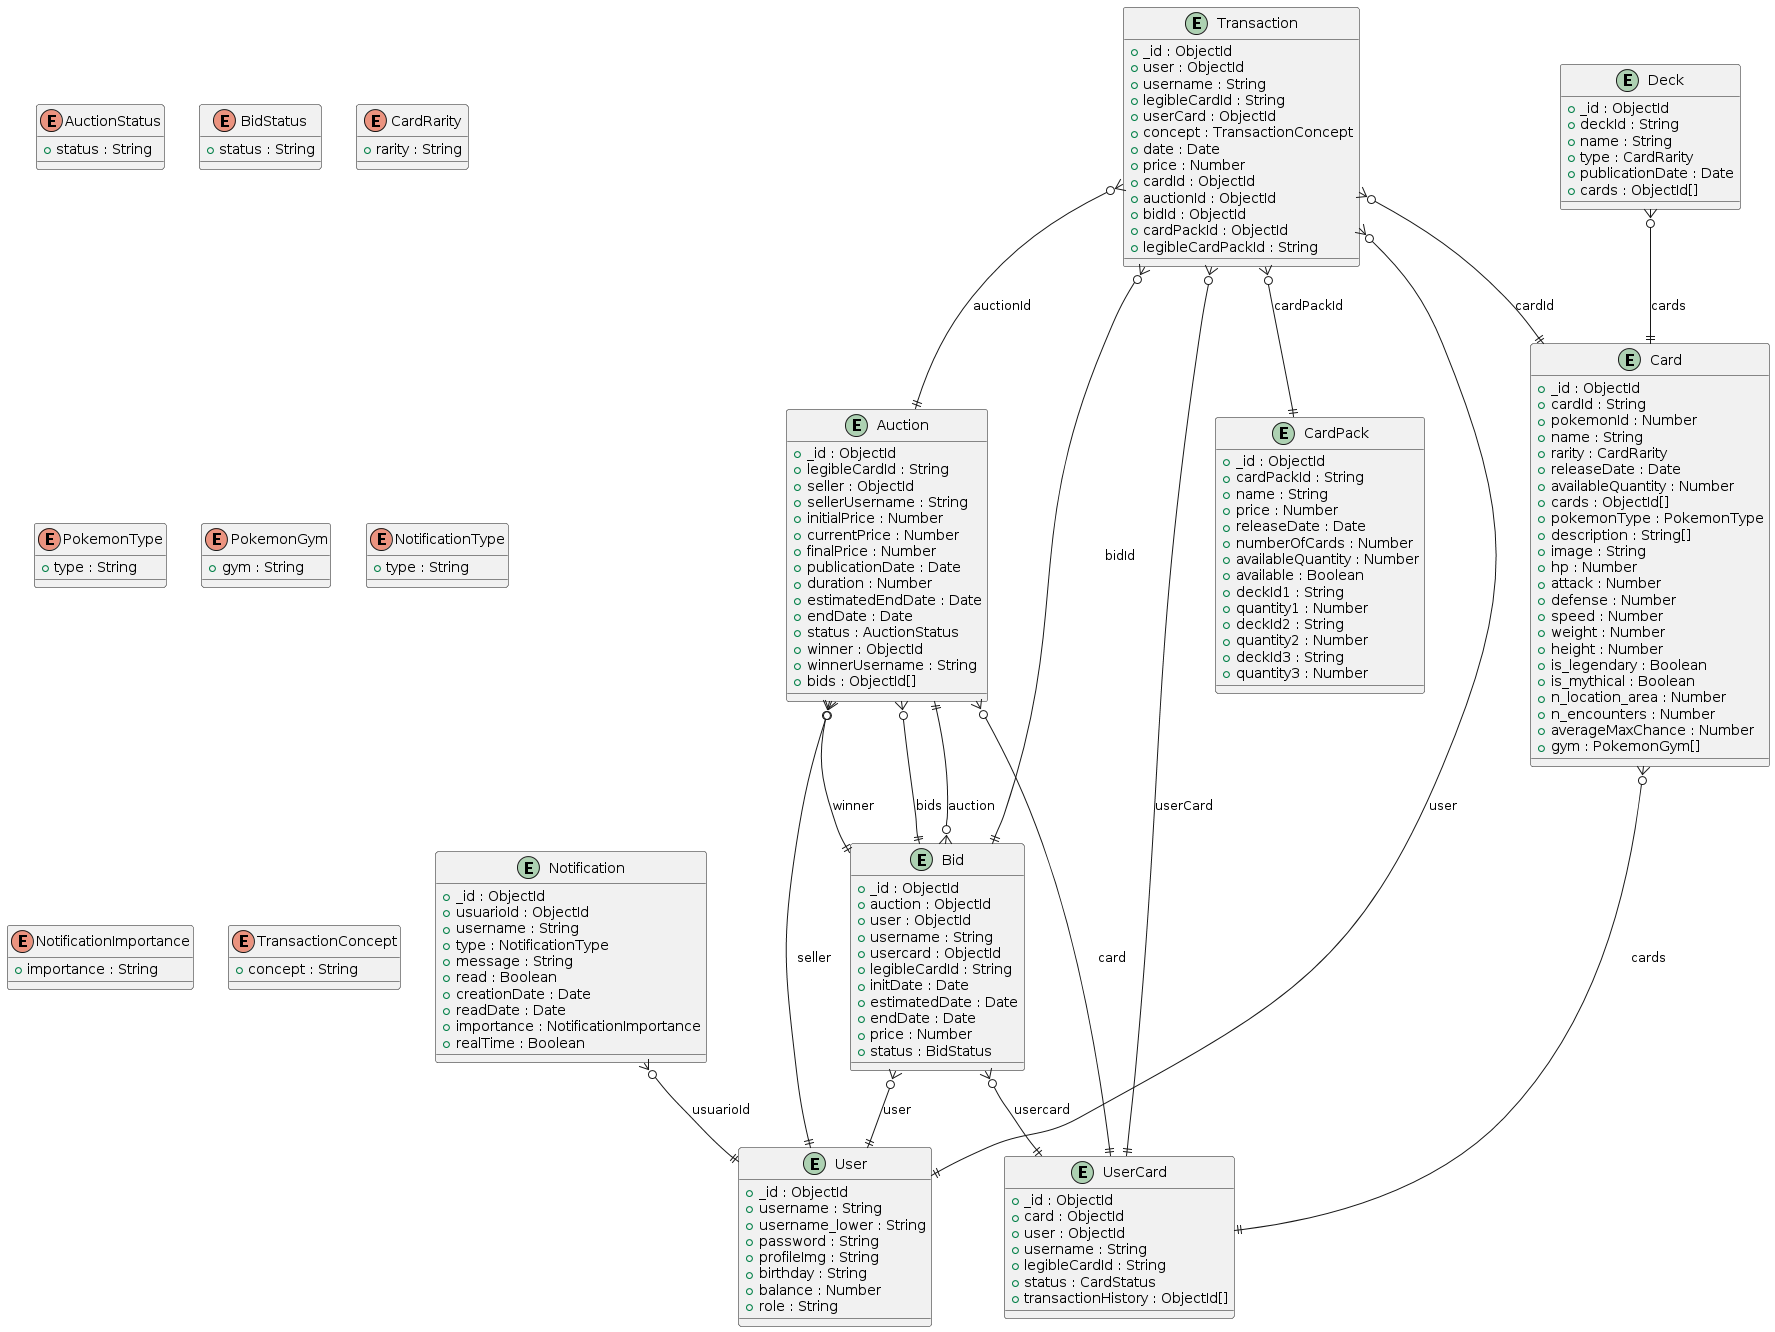
\includegraphics[width=1\textwidth]{figures/6-Analisis/6_9_mongodb_model.png}
    \caption{Modelo de datos de la base de datos MongoDB}
    \label{fig:mongodb_model}
\end{figure}
